% Copyright 2019 by Christian Feuersaenger
%
% This file may be distributed and/or modified
%
% 1. under the LaTeX Project Public License and/or
% 2. under the GNU Free Documentation License.
%
% See the file doc/generic/pgf/licenses/LICENSE for more details.


\section{Externalization Library}
\label{section-libs-external}

{
\pgfkeys{
    /pdflinks/search key prefixes in/.add={/tikz/external/,}{}
}
{\noindent {\emph{by Christian Feuersänger}}}

\begin{tikzlibrary}{external}
    This library provides a high-level automatic or semi-automatic export
    feature for \tikzname\ pictures. Its purpose is to convert each picture to
    a separate \pdf\ without changing the document as such.

    It also externalizes |\label|  information (and other aux file related
    stuff) using auxiliary files.
\end{tikzlibrary}


\subsection{Overview}

There are several reasons why external images for at least some pictures are of
interest:
%
\begin{enumerate}
    \item Larger picture require a considerable amount of time, which is
        necessary for every compilation. However, only few images will change
        from run to run. It can simply save time to export finished images and
        include them as final graphics.
    \item It may be desirable to have final images for some graphics, for
        example to include them in third--party programs or to communicate them
        electronically.
    \item It may be necessary to typeset a file in environments where \pgfname\
        and \tikzname\ are not available. In this case, external images are the
        only way to ensure compatibility.
\end{enumerate}
%
The purpose of this library is to provide a way to export any \tikzname-picture
to separate \pdf\ (or \eps) images without changing the main document. It is
actually a simple user interface to the |\beginpgfgraphicnamed| $\dotsc$
|\endpgfgraphicnamed| framework of \pgfname\ which is discussed in
section~\ref{section-external}.


\subsection{Requirements}

For most users, the library does not need special attention since requirements
are met anyway. It collects all tokens between |\begin{tikzpicture}| and the
next following |\end{tikzpicture}| and replaces them by the appropriate
graphics or it takes steps to generate such an image.
%For Con\TeX t and plain \TeX\ users, the appropriate begin and end picture
%statements apply.

It can't expand macros during this step, so the only requirement is that every
picture's end is directly reachable from its beginning, without further macro
expansion. Furthermore, the library assumes that all \LaTeX\ pictures are ended
with |\end{tikzpicture}|.
%In Con\TeX t, the end command is assumed to be |\stoptikzpicture| and for plain
%\TeX\ it is |\endtikzpicture|.

The library always searches for the \emph{next} picture's end,
|\end{tikzpicture}|. As a consequence, you can't use nested pictures directly.
You \emph{can} nest pictures, but you have to avoid that the nested picture's
|\end| command is found before the outer |\end| command (for example using
bracing constructs or by writing the nested picture into a separate macro
call).

Consider using the |\tikzexternaldisable| method in case you'd like to skip
selected pictures which do not meet the requirements.


\subsection{A Word About Con\TeX t And Plain \TeX}

Currently, the basic layer backend |\beginpgfgraphicnamed| $\dotsc$
|\endpgfgraphicnamed| relies on \LaTeX\ only, so externalization is currently
only supported for \LaTeX.
%The library comes in three different versions, one for \LaTeX, one for Con\TeX
%t and one for plain \TeX. For reasons of simplicity, examples in this manual
%only refer to \LaTeX\ (especially |pdflatex|).


\subsection{Externalizing Graphics}

After loading the library, a call to |\tikzexternalize| is necessary to
activate the externalization.
%
\begin{codeexample}[code only]
\documentclass{article}
% main document, called main.tex
\usepackage{tikz}

\usetikzlibrary{external}
\tikzexternalize % activate!

\begin{document}
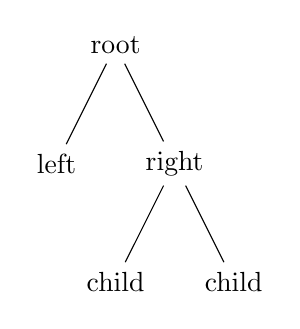
\begin{tikzpicture}
  \node {root}
    child {node {left}}
    child {node {right}
      child {node {child}}
      child {node {child}}
    };
\end{tikzpicture}

A simple image is \tikz \fill (0,0) circle(5pt);.
\end{document}
\end{codeexample}

The method works as follows: if the document is typeset normally, the library
searches for replacement images for every picture. Filenames are generated
automatically in the default configuration. In our case, the two file names
will be |main-figure0| and |main-figure1|. If they exist, those images are
simply included and the pictures as such are not processed. If graphics files
do not exist, steps are taken to generate the missing ones. Since (currently)
only one output file can be set, each missing image needs to be generated by a
separate run of \LaTeX\ in which the |\jobname| is set to the desired image
file name. In the default configuration |mode=convert with system call|, these
commands are issued automatically by using the |\write18| method to call system
commands. It is also possible to output every required file name or to generate
a |makefile|; users will need to issue the required commands manually (or with
|make|). The probably most comfortable way is to use the default configuration
with
%
\begin{codeexample}[code only, tikz syntax=false]
pdflatex -shell-escape main
\end{codeexample}
%
\noindent which authorizes |pdflatex| to call itself recursively to generate
the images. When it finishes, all images are generated and the document already
includes them.

From this point on, successive runs of \LaTeX\ will use the final graphics
files, the pictures won't be used anymore.
Section~\ref{section-libs-external-nopgf} contains details about how to submit
such a file to environments where \pgfname\ is not available.

\begin{command}{\tikzexternalize\oarg{optional arguments}}
    This command activates the externalization. It installs commands to replace
    every \tikzname-picture. It needs to be called before |\begin{document}|
    because it may need to install its separate shipout routine.

    The \meta{optional arguments} can be any of the keys described below.

    Note that the generation/modification of auxiliary files like |.aux|,
    |.toc| etc.\ is usually suppressed while a single image is externalized
    (details for |\label| support follow).

    It is also possible to write |\tikzexternalize|\marg{main job name} if the
    argument is delimited by curly braces. This case is mainly for backwards
    compatibility and is no longer necessary. Since it might be useful in rare
    circumstances, it is documented in section~\ref{sec:external:detail}.

    A detailed description about the process of externalization is provided in
    section~\ref{sec:external:detail}.

    \begin{command}{\tikzexternalrealjob}
        After the library is loaded, this macro will \emph{always} contain the
        correct main job's name (in the example above, it is |main|). It is to
        be used instead of |\jobname| when the externalization is in effect.
    \end{command}
    %
    \begin{command}{\pgfactualjobname}
        Once |\tikzexternalize| has been called, |\pgfactualjobname| contains
        the name of the currently generated output file (which may be |main| or
        |main-figure0| or |main-figure1| in our example above).
    \end{command}
    %
    \begin{command}{\jobname}
        The value of |\jobname| is one of |\tikzexternalrealjob| or
        |\pgfactualjobname|, depending on the configuration. In short: if
        auxiliary file support (|\label| and |\ref|) is activated,
        |\jobname=\tikzexternalrealjob| (since that's the base file name of
        auxiliary files).
    \end{command}
\end{command}

\begin{key}{/tikz/external/system call=\marg{template}}
\label{extlib:systemcall:option}
    A template string used to generate system calls. Inside of \marg{template},
    the macro |\image| can be used as placeholder for the image which is about
    to be generated while |\texsource| contains the main file name (in truth,
    it contains |\input|\marg{main file name}, but that doesn't matter).

    The default depends on the value of |\pgfsysdriver|. For
    |pgfsys-pdftex.def|, it is
    %
\begin{codeexample}[code only]
\tikzset{external/system call={pdflatex \tikzexternalcheckshellescape -halt-on-error
    -interaction=batchmode -jobname "\image" "\texsource"}}
\end{codeexample}
    %
    \noindent where \declareandlabel{\tikzexternalcheckshellescape} inserts the
    value of the configuration key |shell escape| if and only if the current
    document has been typeset with |-shell-escape|\footnote{Note that this is
    always true for the default configuration. This security consideration
    applies mainly for \texttt{mode=list and make} which will also work
    \emph{without} shell escapes.}.

    Other drivers result in slightly different calls. There is support for
    |lualatex|, |xelatex|, and |dvips|. The precise values are written to the
    |.log| file as soon as you attempt to compile a document.

    The argument \marg{template} will be expanded using |\edef|, so any control
    sequences will be expanded. During this evaluation, `|\\|' will result in a
    normal backslash, `|\|'. Furthermore, double quotes `|"|', single quotes
    `|'|', semicolons and dashes `|-|' will be made to normal characters if any
    package uses them as macros. This ensures compatibility with the |german|
    package, for example.
\end{key}

\begin{key}{/tikz/external/shell escape=\marg{command-line arg} (initially -shell-escape)}
    Contains the command line option for |latex| which enables the |\write18|
    feature. For \TeX-Live, this is |-shell-escape|. For MiK\TeX, you should
    use |\tikzexternalize[shell escape=-enable-write18]|.
\end{key}


\subsubsection{Support for Labels and References In External Files}

The |external| library comes with extra support for |\label| and |\ref| (and
other commands which usually store information in the |.aux| file) inside an
external files.

In particular, it supports the two use-cases
%
\begin{enumerate}
    \item[a)] |\ref| to something in the main document inside an externalized
        graphics or
    \item[b)] |\label| in the externalized graphics which is referenced in the
        main document.
\end{enumerate}

The only restriction is that you need to compile your document multiple times
(as usual for references).

\paragraph{NOTE:}
support for a) is unavailable for versions up to and including \pgfname\ 3.0.1.

\begin{key}{/tikz/external/aux in dpth=\marg{boolean} (initially true)}
    Allows to enable or disable the feature which handles references and labels
    as part of image externalization. Disabling it will safe one |\newwrite|
    command, i.e.\ a write register.

    Also see the |disable dependency files| feature.

    Here are some implementation details on how references within/from external
    graphics work for those who would like to know the details:

    For point a), a |\ref| inside of an externalized graphics works by reading
    the main document's |.aux| file. To this end, the standard
    |mode=convert with system call| detects such references and reschedules the
    externalization to |\end{document}.|\footnote{Note that this requires the
    \texttt{atveryend} package. The purpose to reschedule the externalization
    is to access the main job's aux file, but only after it has been written
    completely.} Other values of |mode| require just one attempt to externalize
    the picture.

    Note that |\pageref| is not supported (sorry).

    Point b) works as follows: a |\label| inside of an externalized graphics
    causes the |external| library to generate separate auxiliary files for every
    external image. These files are called \meta{imagename}|.dpth|. The
    extension |.dpth| indicates that the file also contains the image's depth
    (the |baseline| key of \tikzname). Furthermore, anything which would have
    been written to an |.aux| file will be redirected to the |.dpth| file --
    but only things which occur inside of the externalized |tikzpicture|
    environment. When the main document loads the image, it will copy the
    |.dpth| file into the main |.aux| file. Then, successive compilations of
    the main document contain the external |\label| information. In other
    words, a |\label| in an external graphics needs the following work flow:
    %
    \begin{enumerate}
        \item The external graphics needs to be generated together with its
            |.dpth| (usually automatically by \tikzname).
        \item The main document includes the external graphics and copies the
            |.dpth| content into its main |.aux| file.
        \item The main document needs to be translated once again to re-read
            its |.aux| file\footnote{Note that it is not possible to activate
            the content of an auxiliary file after \texttt{\textbackslash
            begin\{document\}} in \LaTeX.}.
    \end{enumerate}

    This does also work if a |\label|/|\ref| combination is implemented itself
    by a |tikzpicture| (a feature offered by |pgfplots|).
\end{key}


\subsubsection{Customizing the Generated File Names}

The default filename for externalized graphics is `\meta{real file
name}|-figure_|\meta{number}' where \meta{number} ranges from $0$ to whatever
is required. However, there are a couple of ways to change the generated
filenames:
%
\begin{itemize}
    \item Changing the overall file name using a |prefix|,
    \item Changing the file name for a single figure using
        |\tikzsetnextfilename|,
    \item Changing the file name for a restricted set of figures using
        |figure name|.
\end{itemize}

\begin{key}{/tikz/external/prefix=\marg{file name prefix} (initially empty)}
    A shortcut for |\tikzsetexternalprefix|\marg{file name prefix}, see below.
\end{key}

\begin{command}{\tikzsetexternalprefix\marg{file name prefix}}
    Assigns a common prefix used by all file names. For example,
    %
\begin{codeexample}[code only]
\tikzsetexternalprefix{figures/}
\end{codeexample}
    %
    will prepend |figures/| to every external graphics file name.

    Please note that |\tikzsetexternalprefix| is the \emph{only} way to assign
    a prefix in case you want to prepare your document for environments where
    \pgfname\ is not installed (see section~\ref{section-libs-external-nopgf}).
\end{command}

\begin{command}{\tikzsetnextfilename\marg{file name}}
    Sets the file name for the \emph{next} \tikzname\ picture or |\tikz| short
    command. It will \emph{only} be used for the next picture.

    Pictures for which no explicit file name has been set (or the next file
    name is empty) will get automatically generated file names.

    Please note that |prefix| will still be prepended to \marg{file name}.
    %
\begin{codeexample}[code only]
\documentclass{article}
% main document, called main.tex
\usepackage{tikz}

\usetikzlibrary{external}
\tikzexternalize[prefix=figures/] % activate

\begin{document}

\tikzsetnextfilename{trees}
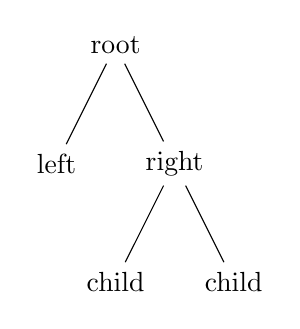
\begin{tikzpicture} % will be written to 'figures/trees.pdf'
  \node {root}
    child {node {left}}
    child {node {right}
      child {node {child}}
      child {node {child}}
    };
\end{tikzpicture}

\tikzsetnextfilename{simple}
A simple image is \tikz \fill (0,0) circle(5pt);. % will be written to 'figures/simple.pdf'


\begin{tikzpicture} % will be written to 'figures/main-figure0.pdf'
   \draw[help lines] (0,0) grid (5,5);
\end{tikzpicture}
\end{document}
\end{codeexample}
    %
\begin{codeexample}[code only, tikz syntax=false]
pdflatex -shell-escape main
\end{codeexample}
    %
\end{command}

\begin{key}{/tikz/external/figure name=\marg{name}}
    Same as |\tikzsetfigurename|\marg{name}.
\end{key}

\begin{command}{\tikzsetfigurename\marg{name}}
    Changes the names of \emph{all} following figures. It is possible to change
    |figure name| during the document either using
    |\tikzset{external/figure name|=\marg{name}|}| or with this command. A
    unique counter will be used for each different \marg{name}, and each
    counter will start at $0$.

    The value of |prefix| will be applied after |figure name| has been
    evaluated.
    %
\begin{codeexample}[code only]
\documentclass{article}
% main document, called main.tex
\usepackage{tikz}

\usetikzlibrary{external}
\tikzexternalize % activate

\begin{document}

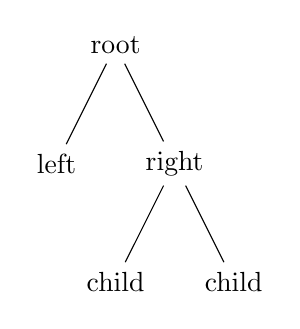
\begin{tikzpicture} % will be written to 'main-figure0.pdf'
  \node {root}
    child {node {left}}
    child {node {right}
      child {node {child}}
      child {node {child}}
    };
\end{tikzpicture}

{
  \tikzsetfigurename{subset_}
  A simple image is \tikz \fill (0,0) circle(5pt);. % will be written to 'subset_0.pdf'

  
\begin{tikzpicture} % will be written to 'subset_1.pdf'
     \draw[help lines] (0,0) grid (5,5);
  \end{tikzpicture}
}% here, the old file name will be restored:

\begin{tikzpicture} % will be written to 'main-figure1.pdf'
   \draw (0,0) -- (5,5);
\end{tikzpicture}
\end{document}
\end{codeexample}
    %
    The scope of |figure name| ends with the next closing brace.

    Remark: Use |\tikzset{external/figure name/.add={prefix_}{_suffix_}}| to
    add a |prefix_| and a |_suffix_| to the actual value of |figure name|.
\end{command}

\begin{command}{\tikzappendtofigurename\marg{suffix}}
    Appends \meta{suffix} to the actual value of |figure name|.

    It is a shortcut for |\tikzset{external/figure name/.add={}|\marg{suffix}|}|
    (a shortcut which is also supported if \tikzname\ is not installed, see
    below).
\end{command}


\subsubsection{Remaking Figures or Skipping Figures}

\begin{command}{\tikzpicturedependsonfile\marg{file name}}
    Adds a dependency for the \emph{next} picture which is about to be
    externalized. If the command is invoked within a picture environment, it
    adds a dependency for the surrounding picture. Dependencies are written
    into \meta{target file}|.dep| in the format

    \meta{target file}|.\tikzexternalimgextension: |\meta{file name}.

    The effect is that if \meta{file name} changes, the external graphics
    associated with the picture shall be remade.

    This command uses the contents of
    \declareandlabel{\tikzexternalimgextension} to check for graphics. If you
    encounter difficulties with image extensions, consider redefining this
    macro (after |\tikzexternalize|).

    \paragraph{Limitations:}
    this command is currently only supported for |mode=list and make| and the
    generated |makefile|.
\end{command}

\begin{command}{\tikzexternalfiledependsonfile\marg{external graphics}\marg{file name}}
    A variant of |\tikzpicturedependsonfile| which adds a dependency for an
    \meta{external graphics}. The argument \meta{external graphics} must be the
    path as it would have been generated by the |external| library, i.e.\ without
    file extension but including any prefixes.
\end{command}

\begin{key}{/tikz/external/disable dependency files}
    Allows to (irreversibly) disable the generation of file dependencies.
    Disabling it will safe one |\newwrite| command, i.e.\ a write register.
    Note that the write register is only allocated if the feature has been used
    at all. This key needs to be provided as argument to |\tikzexternalize| (or
    it needs to be set before calling |\tikzexternalize|).

    Also see the |aux in dpth| key.
\end{key}

\begin{key}{/tikz/external/force remake=\marg{boolean} (default true)}
    A boolean which is used to customize the up-to-date checks of all following
    figures. Every up-to-date check will fail, resulting in automatic
    regeneration of every following figure.
    %
\begin{codeexample}[code only]
\tikzset{external/force remake}

\begin{tikzpicture}
    \draw (0,0) circle(5pt);
\end{tikzpicture}
\end{codeexample}
    %
    You can also use |force remake| inside of a local \TeX\ group to remake
    only selected pictures. The example
    %
\begin{codeexample}[code only]
\tikz \draw (0,0) -- (1,1);

{
\tikzset{external/force remake}

\begin{tikzpicture}
   \draw (0,0) circle(5pt);
\end{tikzpicture}
}

\tikz \draw (0,0) -- (1,1);
\end{codeexample}
    will only apply |force remake| to the second figure.

    Up-to-date checks are applied for |mode=convert with system call| and the
    makefile generated by |mode=list and make|.
\end{key}

\begin{key}{/tikz/external/remake next=\marg{boolean} (default true)}
    A variant of |force remake| which applies only to the next image.
\end{key}

\begin{key}{/tikz/external/export next=\marg{boolean} (default true)}
    A boolean which can be used to disable the export mechanism for single pictures.
\end{key}

\begin{key}{/tikz/external/export=\marg{boolean} (initially true)}
    A boolean which can be used to disable the export mechanism for all
    pictures inside of the current \TeX-scope.
    %
\begin{codeexample}[code only]
\begin{document}
\begin{tikzpicture} % will be exported
    ...
\end{tikzpicture}

{
\tikzset{external/export=false}
\begin{tikzpicture} % won't be exported
    ...
\end{tikzpicture}
...
}

\begin{tikzpicture} % will be exported
    ...
\end{tikzpicture}
\end{document}
\end{codeexample}
    %
    For \LaTeX, the feature lasts until the next |\end|\marg{$\cdot$} (this
    holds for every call to |\tikzset|).
\end{key}

\begin{key}{/tikz/external/up to date check=\marg{choice} (initially md5)}
    The |external| lib has to decide when some existing figure is up-to-date.
    In such a case, it can be used without remaking it. Outdated pictures will
    be remade.

    The key |up to date check| allows to choose among a couple of heuristics
    which are supposed to catch the most important reasons to remake a figure.

    The |up to date check| can be overrule by any of the |force remake| or
    |remake next| keys: if one of them is true, the figure is not up-to-date.

    The choice \declare{simple} is based on the existence of the file: the file
    is up-to-date if and only if it exists.

    The choice \declare{md5} generates an MD5 checksum of the picture for which
    the up-to-date check is running. The MD5 is compared against the MD5 of the
    previous run, which, in turn, will be written into an extra file with the
    extension |.md5|. This file will be modified if and only if the MD5
    comparison indicates a difference. The MD5 computation is based on the
    pdf\TeX\ method |\pdfmdfivesum|. If it is unavailable for some reason, the
    choice |diff| will be used instead.

    The choice \declare{diff} is the same as MD5 -- except that it compares the
    picture content as-is instead of a hash. The |.md5| file will be used to
    compare an old version with the current one -- but its content is some
    ``normalized'' version of the picture for internal use.

    \paragraph{Attention:}
    the content--based strategies |md5| and |diff| operate on the picture
    content -- and only on the picture content. Here, ``picture content'' only
    includes the top--level tokens; no expansion is applied and no included
    files are part of the strategies. If you change preamble styles, you have
    to rebuild the figures manually (for example by deleting the generated
    graphics files). If you have include files, consider using
    |\tikzpicturedependsonfile| and its variants. Since this key provides
    heuristics, you should always remake your figures before you finally
    publish your document. Example: Suppose we have the following picture which
    depends on a command |\mycommand|:
    %
\begin{codeexample}[code only]
\def\mycommand{My comment}

\begin{tikzpicture}

\node at (0,0) {\mycommand};

\end{tikzpicture}
\end{codeexample}
    %
    What happens if you change ``My comment'' to ``My super comment''? Well,
    |external| will \emph{not} pick it up; you will need to handle this
    manually. However, if you modify anything between |\begin{tikzpicture}| and
    |\end{tikzpicture}|, the |external| library \emph{will} pick it up and
    regenerate the picture.

    The |up to date check| is applied for |mode=convert with system call| and
    |mode=list and make|.
\end{key}

\begin{command}{\tikzexternaldisable}
    Allows to disable the complete externalization. While |export next| will
    still collect the contents of picture environments, this command uninstalls
    the hooks for the |external| library completely. Thus, nested picture
    environments or environments where |\end{tikzpicture}| is not directly
    reachable won't produce compilation failures -- although it is not possible
    to externalize them automatically.

    The externalization remains disabled until the end of the next \TeX\ group
    (or environment) or until the next call to |\tikzexternalenable|.
\end{command}

\begin{command}{\tikzexternalenable}
    Re-enables a previously running externalization after |\tikzexternaldisable|.
\end{command}


\subsubsection{Customizing the Externalization}

\begin{key}{/tikz/external/figure list=\marg{boolean} (initially true)}
    A boolean which configures whether a figure list shall be generated. A
    figure list is an output file named \marg{jobname}|.figlist| which is
    filled with file names of each figure, one per line.

    This file is not used by \TeX\ anymore, its purpose is to issue the
    required conversion commands |pdflatex -jobname |\marg{picture file name}
    \marg{main file} manually (or in a script). See
    section~\ref{sec:external:detail} for the details about the expected system
    call (or activate |mode=convert with system call| and inspect your log
    file).
    %
\begin{codeexample}[code only]
\documentclass{article}
% main document, called main.tex
\usepackage{tikz}

\usetikzlibrary{external}
\tikzexternalize[
   mode=graphics if exists,
   figure list=true,
   prefix=figures/]

\begin{document}

\tikzsetnextfilename{trees}
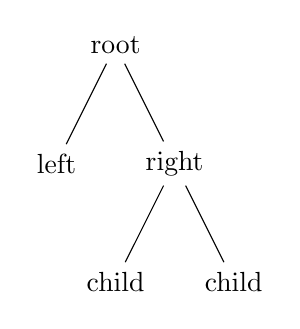
\begin{tikzpicture}
  \node {root}
    child {node {left}}
    child {node {right}
      child {node {child}}
      child {node {child}}
    };
\end{tikzpicture}

\tikzsetnextfilename{simple}
A simple image is \tikz \fill (0,0) circle(5pt);.


\begin{tikzpicture}
   \draw[help lines] (0,0) grid (5,5);
\end{tikzpicture}
\end{document}
\end{codeexample}

\begin{codeexample}[code only, tikz syntax=false]
pdflatex main
\end{codeexample}
    %
    generates |main.figlist| containing
    %
\begin{codeexample}[code only, tikz syntax=false]
figures/trees
figures/simple
figures/main-figure0
\end{codeexample}
    %
\end{key}

\begin{key}{/tikz/external/mode=\marg{choice} (initially convert with system call)}
    Configures what to do with \tikzname\ pictures (unless we are currently
    externalizing one particular image, in that case, these modes are ignored).

    The preconfigured mode |convert with system call| checks whether external
    graphics files are up-to-date and includes them if that is the case. Any
    picture which is not up-to-date will be generated automatically using a
    system call. The system call can be configured using the |system call|
    template. The up-to-date check is applied according to the
    |up to date check| key. As soon as |convert with system call| is set, the
    |figure list| will be disabled -- such a file is not required. In case you
    still need or want it, you can enable it after setting |mode|.

    Please note that system calls may be disabled for security reasons. For
    pdflatex, they can be enabled using
    %
\begin{codeexample}[code only, tikz syntax=false]
pdflatex -shell-escape
\end{codeexample}
    %
    while other \TeX\ variants may need other switches. The feature is
    sometimes called |\write18|.

    The choice |only graphics| always tries to replace pictures with external
    graphics. It is an error if the graphics file does not exist.

    The choice |no graphics| (or, equivalently, |only pictures|) typesets
    \tikzname\ pictures without checking for external graphics.

    A mixture is |graphics if exists|, it checks whether a suitable graphics
    file exists and includes it if that is the case. If it does not exist, the
    picture is typeset using \TeX.

    Mode |list only| skips every \tikzname\ picture; it only generates the file
    \marg{main file}|.figlist| containing file names for every picture, the
    contents of any picture environment is thrown away and a replacement text
    is shown. This implies |figure list=true|. See also the |list and make|
    mode which includes available graphics.

    The mode |list and make| is similar to |list only|: it generates the same
    file \marg{main file}|.figlist|, but any images which exist already are
    included as graphics instead of ignoring them. Furthermore, this mode
    generates an additional file: \marg{main file}.makefile. This allows to use
    a work flow like
    %
\begin{codeexample}[code only, tikz syntax=false]
% step 1: generate main.makefile:
pdflatex main
% step 2: generate ALL graphics on 2 processors:
make -j 2 -f main.makefile
% step 3: include the graphics:
pdflatex main
\end{codeexample}
    %
    \noindent This last make method is optional: |list and make| just assumes
    that images are generated somehow (not necessarily with the generated
    makefile). The generated makefile allows parallel externalization of
    graphics on multi-core systems and it supports any file dependencies
    configured with |\tikzpicturedependsonfile|. Furthermore, it respects the
    |force remake| and |remake next| keys.
\end{key}

\begin{key}{/tikz/external/verbose IO=\marg{boolean} (initially true)}
    A boolean which configures whether I/O operations shall be listed in the
    logfile.
\end{key}

\begin{key}{/tikz/external/verbose optimize=\marg{boolean} (initially true)}
    A boolean which configures whether optimization operations shall be listed
    in the logfile.
\end{key}

\begin{key}{/tikz/external/verbose=\marg{boolean} (initially true)}
    Sets all verbosity flags to \meta{boolean}.
\end{key}

\begin{key}{/tikz/external/optimize=\marg{boolean} (initially true)}
    Configures whether the conversion process shall be optimized. This affects
    only the case when |\jobname| differs from the main file name, i.e.\ when
    single pictures are converted.

    In that case, the main file is compiled as usual -- but everything except
    the selected picture is thrown away. If optimization is enabled, all other
    pictures won't be processed at all. Furthermore, expensive commands which
    do not contribute to the selected picture will be thrown away as well.

    The default implementation discards |\includegraphics| commands which are
    \emph{not} inside of the selected picture to reduce conversion time.

    It is possible to add commands which shall be optimized away, see below.
\end{key}

\begin{key}{/tikz/external/optimize command away=\meta{\textbackslash command}\marg{required argument count}}
    Installs commands to optimize \meta{\textbackslash command} away. As is
    described above, optimization applies to the case when single pictures are
    converted: one usually doesn't need to process (probably expensive)
    commands which do not contribute to the selected picture.

    The argument \marg{required argument count} is either empty or a
    non-negative integer between $0$ and $9$. It denotes the number of
    arguments which should be consumed after \meta{\textbackslash command}. In
    any case, one argument in square brackets after the command will be
    recognized as well. To be more precise, the following cases for arguments
    of \meta{\textbackslash command} are supported:
    %
    \begin{enumerate}
        \item If \marg{required argument count} is empty (the default),
            \meta{\textbackslash command} may take one optional argument in
            square brackets and one in curly braces (which is also optional).
        \item If \marg{required argument count} is not empty,
            \marg{\textbackslash command} may take one optional argument in
            square brackets. Furthermore, it expects exactly \marg{required
            argument count} following arguments.
    \end{enumerate}

    Example:
    %
\begin{codeexample}[code only]
\tikzset{external/optimize command away=\includegraphics}
\end{codeexample}

\begin{codeexample}[code only]
\newcommand{\myExpensiveMacro}[1]{Very expensive!}

\tikzset{external/optimize command away=\myExpensiveMacro}
\end{codeexample}

\begin{codeexample}[code only]
\newcommand{\myExpensiveMacroWithThreeArgs}[3]{Very expensive!}

\tikzset{external/optimize command away={\myExpensiveMacroWithThreeArgs}{3}}
\end{codeexample}

\begin{codeexample}[code only]
% A command with optional argument:
\newcommand{\aFurtherExample}[3][]{Very expensive!}

% consume only two arguments: the first optional one will be processed
% anyway:
\tikzset{external/optimize command away={\myExpensiveMacroWithThreeArgs}{2}}
\end{codeexample}
    %
    The argument \meta{\textbackslash command} must be the name of a single
    macro. Any occurrence of this macro, together with its arguments, will be
    removed.
    %
\begin{codeexample}[code only]
\begin{tikzpicture}
    % this picture is currently converted!
\end{tikzpicture}

This here is outside of the converted picture and contains \myExpensiveMacro. It will be discarded.

This call: \myExpensiveMacro[argument=value]{Argument} as well.
And this here: \myExpensiveMacro{Argument} also.
\end{codeexample}

    The default is to optimize |\includegraphics| away.

    This key is actually a style which sets the |optimize/install| and
    |optimize/restore| keys.
\end{key}

\begin{key}{/tikz/external/optimize/install}
    A command key which contains code to install optimizations. You can append
    code here (or clear the macro) if you need to modify the optimization.
\end{key}

\begin{key}{/tikz/external/optimize/restore}
    A command key which contains code to undo optimizations. You can append
    code here (or clear the macro) if you need to modify the optimization.
\end{key}

\begin{key}{/tikz/external/only named=\marg{boolean} (initially false)}
    If enabled, only pictures for which file names have been set explicitly
    using |\tikzsetnextfilename| will be considered, no file names will be
    generated automatically.
\end{key}

\begin{key}{/pgf/images/include external (initially \textbackslash pgfimage\{\#1\})}
\index{External Graphics!Bounding Box Issues}
    This command key constitutes the public interface to exchange the
    |\includegraphics| command used for the image inclusion. If can be
    overwritten using |include external/.code=|\marg{\TeX\ code}.

    Its description can be found in the corresponding basic layer documentation
    on page~\pageref{pgf:includeexternalkey}.

    Just one example here: you can use
    %
\begin{codeexample}[code only]
\pgfkeys{/pgf/images/include external/.code={\includegraphics[viewport=0 0 211.28 175.686]{#1}}}
\end{codeexample}
    %
    to manually change the viewport (bounding box) for included graphics.

    Another example (of probably limited use) is
    %
\begin{codeexample}[code only]
\pgfkeys{/pgf/images/include external/.code={\href{file:#1}{\pgfimage{#1}}}}
\end{codeexample}
    %
    \noindent which will generate a clickable hyperlink around the image.
    Clicking on it opens the single exported file\footnote{This requires all
    external graphics files in the same base directory as the main |.pdf|
    file.}.

    If you want to limit the effects of this key to just one externalized
    figure, use
    %
\begin{codeexample}[code only]
{
  \pgfkeys{/pgf/images/include external/.code={\includegraphics[viewport=0 0 211.28 175.686]{#1}}}
  \begin{tikzpicture}
     ...
  \end{tikzpicture}
}% this brace ends the effect of `include external'
\end{codeexample}
    %
\end{key}

\begin{command}{\tikzifexternalizing\marg{true code}\marg{false code}}
    This command can be used to check whether an image is currently written to
    its separate graphics file (if the ``grab'' procedure is running). If so,
    the \marg{true code} will be executed. If not, that means if the main
    document is being typeset normally, the \marg{false code} will be invoked.

    This command must be used \emph{after} |\tikzexternalize|.
\end{command}

\begin{command}{\tikzifexternalizingnext\marg{true code}\marg{false code}}
    Like |\tikzifexternalizing|, but this variant also checks if the next
    following figure is the one which is about to be written to its separate
    graphics file.
\end{command}


\subsubsection{Details About The Process}
\label{sec:external:detail}

The standard run |pdflatex |\meta{main document} causes the |external| library
to check every occurrence of |\begin{tikzpicture}| and every |\tikz| short
command. If it finds a picture which shall be exported, it queries the
respective file name and checks whether the file exists already. If so, it
includes the external graphics. If not, it requires an externalization which
can be done automatically (the default), semi-automatically (with
|mode=list and make|) or manually (by issuing the requires system calls
somehow).

The library can detect whether it runs in ``conversion mode'', i.e.\ if it
should only process a single image. To do so, it checks whether the internal
macro \declareandlabel{\tikzexternalrealjob} exists. If so, its contents is
assumed to be \meta{main document} (without the suffix |.tex|). Usually, this
macro is set by the conversion system call,
%
\begin{codeexample}[code only, tikz syntax=false]
pdflatex -jobname "main-figure0" "\def\tikzexternalrealjob{main}\documentclass[x11names]{article}
\usepackage[english]{babel}
\usepackage[T1]{fontenc}
\usepackage[utf8]{inputenc}
\usepackage{figchild}
\usepackage{verbatim}
\usepackage{authblk}
\usepackage{float}
\usepackage{url}
\usepackage{multirow}
\usepackage{multicol}
\usepackage{hyperref}
\usepackage{amsmath,array,booktabs}
\usepackage{afterpage}
\usepackage{geometry}
\geometry{top=2cm, left=2cm, right=2cm, bottom=2cm}
\usepackage[bf]{caption}
\usepackage{aurical}
\usepackage{xcolor}
%\makeatletter
%\newcommand\HUGE{\@setfontsize\Huge{50}{60}}
%\makeatother 
\definecolor{bluetop}{RGB}{24, 24, 181}
\definecolor{bookred}{RGB}{129, 57, 55}



\begin{document}

\begin{titlepage}
\begin{tikzpicture}[remember picture,overlay]
%\draw[line width=1.5pt, cap=round]
%    ([yshift=-1cm]current page.north west) -- ([yshift=-1cm]current page.north east);
\draw[ultra thick, fill= Azure2        ] ( -3, 2)--(-3  ,-2.5)--(0, -2.5)--(0, 2) -- cycle;
\draw[ultra thick, fill= Bisque3       ] (0.5, 2)--(0.5 ,-2.5)--(4, -2.5)--(4, 2) -- cycle;
\draw[ultra thick, fill= CadetBlue1    ] (4.5, 2)--(4.5 ,-2.5)--(8, -2.5)--(8, 2) -- cycle;
\draw[ultra thick, fill= DarkGoldenrod1] (8.5, 2)--(8.5 ,-2.5)--(12,-2.5)--(12,2) -- cycle;
\draw[ultra thick, fill= Firebrick1    ] (12.5,2)--(12.5,-2.5)--(16,-2.5)--(16,2) -- cycle;
\draw[ultra thick, fill= Gold1         ] (16.5,2)--(16.5,-2.5)--(20,-2.5)--(20,2) -- cycle;
\node at (-2.25, -0.25) {\fcOwlA{0.7}{black}{1}};
\node at (2.25, -0.25) {\fcApple{0.7}{black}{2}};
\node at (6.25, -0.25) {\fcBat{0.5}{black}{2}};
\node at (10.25,-0.25) {\fcBear{0.5}{black}{1}};
\node at (14.25,-0.25) {\fcBirdC{0.5}{black}{1}};
\node at (18.25,-0.25) {\fcBoat{0.6}{black}{2}};
\draw[line width=1.5pt, cap=round]
    ([yshift=-5.3cm]current page.north west) -- ([yshift=-5.3cm]current page.north east);
\end{tikzpicture}
\vspace{3cm}
\begin{center}
%\bfseries
\fontsize{23mm}{23mm}\selectfont 
\textcolor{red}{\Fontauri figchild Package}
\end{center}
\vspace{1.5cm}
\begin{tikzpicture}[remember picture,overlay]
\draw[line width=1.5pt, cap=round] 
([yshift=-9.25cm]current page.north west) -- ([yshift=-9.25cm]current page.north east);
\draw[ultra thick, fill= HotPink2] (-3, 0.5) -- (-3 , -3) -- (0, -3) -- (0, 0.5) -- cycle;
\draw[ultra thick, fill= IndianRed1  ] (0.5, 0.5) -- (0.5, -3) -- (4, -3) -- (4, 0.5) -- cycle;
\draw[ultra thick, fill= Khaki1] (4.5, 0.5) -- (4.5, -3) -- (8, -3) -- (8, 0.5) -- cycle;
\draw[ultra thick, fill= LavenderBlush3 ] (8.5, 0.5) -- (8.5 ,-3) -- (12,-3) -- (12,0.5) -- cycle;
\draw[ultra thick, fill= Maroon4 ] (12.5,0.5) -- (12.5,-3) -- (16,-3) -- (16,0.5) -- cycle;
\draw[ultra thick, fill= NavajoWhite2 ] (16.5,0.5) -- (16.5,-3) -- (20,-3) -- (20,0.5) -- cycle;
\draw[line width=1.5pt, cap=round]
    ([yshift=-14.35cm]current page.north west) -- ([yshift=-14.35cm]current page.north east);
\node at (-2.25, -1.25) {\fcBonnet{0.7}{black}{2}};    
\node at (2.25,  -1.25) {\fcBookA{0.6}{black}{1}};
\node at (6.25,  -1.25) {\fcBull{0.5}{black}{1}};
\node at (10.25, -1.25) {\fcButterfly{0.5}{black}{1}};
\node at (14.25, -1.25) {\fcCandle{0.5}{black}{1}};
\node at (18.25, -1.25) {\fcCarrot{0.3}{black}{1}};
\draw[ultra thick, fill=OliveDrab1] (-3 , -4)--(-3 , -7.5)--(0, -7.5)--(0, -4) -- cycle;
\draw[ultra thick, fill=PaleGreen2   ] (0.5, -4)--(0.5, -7.5)--(4, -7.5)--(4, -4) -- cycle;
\draw[ultra thick, fill= RosyBrown4] (4.5, -4)--(4.5, -7.5)--(8, -7.5)--(8, -4) -- cycle;
\draw[ultra thick, fill= SkyBlue1 ] (8.5, -4)--(8.5 ,-7.5)--(12,-7.5)--(12,-4) -- cycle;
\draw[ultra thick, fill= Tomato1 ] (12.5,-4)--(12.5,-7.5)--(16,-7.5)--(16,-4) -- cycle;
\draw[ultra thick, fill= VioletRed1 ] (16.5,-4)--(16.5,-7.5)--(20,-7.5)--(20,-4) -- cycle;
\draw[line width=1.5pt, cap=round]
    ([yshift=-19cm]current page.north west) -- ([yshift=-19cm]current page.north east);
\node at (-2.25, -5.75) {\fcCat{0.8}{black}{1}};
\node at (2.25, -5.75) {\fcCentipede{0.4}{black}{1}};
\node at (6.25, -5.75) {\fcChristmasTree{0.5}{black}{1}};
\node at (10.25,-5.75) {\fcDog{0.5}{black}{1}};
\node at (14.25,-5.75) {\fcDolphin{0.5}{black}{1}};
\node at (18.25,-5.75) {\fcDuck{0.5}{black}{2}};
\draw[ultra thick, fill=Wheat4] (-3 , -8.5)--(-3 , -12)--(0, -12)--(0, -8.5) -- cycle;
\draw[ultra thick, fill=Yellow1   ] (0.5, -8.5)--(0.5, -12)--(4, -12)--(4, -8.5) -- cycle;
\draw[ultra thick, fill= MistyRose4] (4.5, -8.5)--(4.5, -12)--(8, -12)--(8, -8.5) -- cycle;
%\draw[ultra thick, fill= blue ] (8.5, -8.5)--(8.5 ,-12)--(12,-12)--(12,-8.5) -- cycle;
%\draw[ultra thick, fill= pink ] (12.5,-8.5)--(12.5,-12)--(16,-12)--(16,-8.5) -- cycle;
\bfseries
\node at (12.3, -9.5) {{\Huge \textcolor{SteelBlue4}{Figures for Creating}}};
\node at (12.3, -11) {{\Huge \textcolor{SteelBlue4}{Children’s Activities}}};
%\node at (12.3, -11) {{\large Figures for Creating}};
%\node at (12.3, -11.5) {{\large Children’s Activities}};
\draw[ultra thick, fill= gray ] (16.5,-8.5)--(16.5,-12)--(20,-12)--(20,-8.5) -- cycle;
\draw[line width=1.5pt, cap=round]
    ([yshift=-23.5cm]current page.north west) -- ([yshift=-23.5cm]current page.north east);
\draw[line width=1.5pt, cap=round]
    ([yshift=-24.5cm]current page.north west) -- ([yshift=-24.5cm]current page.north east);
\node at (-2.25, -10.25) {\fcElephant{0.7}{black}{1}};
\node at (2.25, -10.25) {\fcFishA{0.7}{black}{1}};
\node at (6.25, -10.25) {\fcFlamingoA{0.7}{black}{1}};
%\node at (10.25,-10.25) {{\HUGE $\awint$}};
%\node at (14.25,-10.25) {{\HUGE $\risingdotseq$}};
\node at (18.25,-10.25) {\fcFlowerB{0.3}{black}{1}};
\draw[ultra thick, fill=Aquamarine1   ] (0.5, -14)--(0.5, -17.5)--(4, -17.5)--(4, -14) -- cycle;
\draw[ultra thick, fill=Tan4] (-3 , -14)--(-3 , -17.5)--(0, -17.5)--(0, -14) -- cycle;
\draw[ultra thick, fill= Plum4] (4.5, -14)--(4.5, -17.5)--(8, -17.5)--(8, -14) -- cycle;
\draw[ultra thick, fill= Ivory1 ] (8.5, -14)--(8.5 ,-17.5)--(12,-17.5)--(12,-14) -- cycle;
\draw[ultra thick, fill= Burlywood2 ] (12.5,-14)--(12.5,-17.5)--(16,-17.5)--(16,-14) -- cycle;
\draw[ultra thick, fill= IndianRed1 ] (16.5,-14)--(16.5,-17.5)--(20,-17.5)--(20,-14) -- cycle;
\node at (-2.25,-15.75) {\fcFlowerF{0.6}{black}{1}};
\node at (2.25, -15.75) {\fcFlyingSaucer{0.6}{black}{1}};
\node at (6.25, -15.75) {\fcFrog{0.5}{black}{1}};
\node at (10.25,-15.75) {\fcGiraffe{0.5}{black}{2}};
\node at (14.25,-15.75) {\fcHouseA{0.6}{black}{1}};
\node at (18.25,-15.75) {\fcLion{0.6}{black}{1}};
\draw[line width=1.5pt, cap=round]
    ([yshift=-29cm]current page.north west) -- ([yshift=-29cm]current page.north east);
\end{tikzpicture}
\end{titlepage}

\thispagestyle{empty}

\begin{center}

\textbf{figchild:} Figures for Creating Children's Activities

\vspace{0.5cm}

\url{https://github.com/fsbmat-ufv/figchild}

\vspace{0.5cm}

\version{2}{1}{1}

\vspace{0.5cm}

\today

\end{center}

\vspace{2cm}



 Fernando de Souza Bastos\footnote{Author and maintainer of the package (\textbf{E-mail:} fernando.bastos@ufv.br)}, 
 Guilherme Fernandes Castro de Oliveira, 
 José Vitor Novaes Moreira,
 Jéssica de Mendonça,
 Gabriel Singh Bruno,
 Matheus Iago Teixeira da Silva,
 Erlane Alves Santiago,
 Ana Carolina de Assis Coelho,
 Lucas Mendes Viana,
 Dhavy Alexwander Lopes dos Santos,
 Vitória Augusta Dutra de Castro Soares,
 Júlia Letícia Gonçalves Martins,
 Kethile Alves Fagundes,
 Luan Moises dos Santos Valadares,
 Luiz Henrique de Souza Matos,
 Warley Ribeiro de Freitas,
 Paula Alves de Freitas,
 Janaíne Geralda Mesquita Martins,
 Henrique Ribeiro Diniz
 
\vspace{3cm}

\noindent \textbf{License:}

\vspace{1cm}

\noindent Copyright 2022 by Fernando de Souza Bastos

\vspace{1cm}

\noindent Released under the LaTeX Project Public License v1.3c or later. See \url{http://www.latex-project.org/lppl.txt}. Feature requests, issues and pull requests are welcome.

\newpage

\begin{abstract}
This package was created with the aim of facilitating the work of Elementary School teachers who need to create colorful and attractive activities for their students. It is a product of the Computational Mathematics discipline offered at the Federal University of Viçosa - Campus UFV - Florestal by professor Fernando de Souza Bastos. It makes use of the tikz and xcolor packages.
\end{abstract}

\tableofcontents

\listoftables

\strut\newpage

\section{Introduction}

\hspace{\parindent}This is a simple package to quickly make figures that can be used to build Basic Education activities. Of course, they can also be used for other purposes. It was created with the help of several students of Computational Mathematics discipline (MAF 172) from figures found in children's activities applied by teachers from Brazil and the world.. All students was added as authors of the package, as they contributed to the construction of the images, after learning how to use the tikz package. The discipline was offered by Professor Fernando de Souza Bastos\footnote{http://lattes.cnpq.br/9772451905214345}, at the Federal University of Viçosa - Campus UFV - Florestal (UFV), in Brazil.

Our goal is to contribute to Teaching and the creation of high quality typographic materials. Thus, we seek to reproduce several images used in lists of activities of Basic Education in Brazil and in the world. That way, the teacher who wants to create activities, does not need to waste hours creating such images or copying low quality images on the internet. Just use our package.

In addition to the images, we have also created some activities that can be copied and used by teachers. The activities are in Portuguese, but in future versions of the package we will also make them available in English.

The package is in a process of constant evolution, whenever possible, we will add other images and content in it. In Tables \ref{tab1} à \ref{tab18} we present all the images created so far. We also intend to add images related to commemorative dates such as Christmas, Easter, Halloween, among others. Enjoy the figchild package.



%\section{Author and Acknowledgements}

%\hspace{\parindent}Fernando de Souza Bastos has a degree in Mathematics from the Federal University %of Viçosa and a PhD in Statistics from the Federal University of Minas Gerais. He has been working %with \LaTeX since 2003.

%Thanks in particular the students Guilherme Fernandes Castro de Oliveira and José Vitor Novaes %Moreira who acted as monitors of the discipline (MAF 172) in the second remote period offered by UFV, %in the year 2021. I also thank all the students who contributed to the creation of the figures.

\section{Usage}

\hspace{\parindent}To use the package, simply add the command to your document's preamble:

\begin{verbatim}
     \usepackage{figchild}
\end{verbatim}

After that, in the body of your text you must use the command of the figure you want with its three options, the first option is related to the size of the figure, the second option is related to color and the third option is related to line thickness of the figure. That is, the command can be indicated as:

\begin{verbatim}
     \imagename{Picture size}{Picture color}{Line thickness}
\end{verbatim}

For example, to create a little train in the center of the page, of size 2, gray color and with line thickness that defines it of size 2, just use:

\begin{verbatim}
    \begin{center}
    \fcTrain{2}{gray}{2}
    \end{center}
\end{verbatim}

\begin{center}
    \fcTrain{2}{gray}{2}
\end{center}

\newgeometry{top=1.5cm, left=2cm, right=2cm, bottom=2cm}
\afterpage{\globaldefs=1 \newgeometry{top=0.5cm, left=0.5cm, right=0.5cm, bottom=2cm}}
%\newpage



\section{Figures}

\begin{table}[H]\centering\begin{tabular}{|c|l|c|}\hline {\bf Command}& \multicolumn{1}{c|}{{\bf Options}} & {\bf Figures}\\  \hline	&&\multirow{5}{*}{\fcAbajourA{0.1}{black}{1}}\\	&&\\	&\verb|#1|: Figure Scale &\\	\verb|\fcAbajourA{#1}{#2}{#3}|&	\verb|#2|: drawing line color &\\	&\verb|#3|: Line thickness (pt) &\\ &&\\&&	\verb|\fcAbajourA{0.1}{black}{1}|\\\hline 	
	&&\multirow{5}{*}{\fcAbajourB{0.1}{black}{1}}\\	&&\\	&\verb|#1|: Figure Scale &\\	\verb|\fcAbajourB{#1}{#2}{#3}|&	\verb|#2|: drawing line color &\\	&\verb|#3|: Line thickness (pt) &\\ &&\\&&	\verb|\fcAbajourB{0.1}{black}{1}|\\\hline 	
	&&\multirow{5}{*}{\fcAbajourC{0.1}{black}{1}}\\	&&\\	&\verb|#1|: Figure Scale &\\	\verb|\fcAbajourC{#1}{#2}{#3}|&	\verb|#2|: drawing line color &\\	&\verb|#3|: Line thickness (pt) &\\ &&\\&&	\verb|\fcAbajourC{0.1}{black}{1}|\\\hline 	
	&&\multirow{5}{*}{\fcAbajourD{0.1}{black}{1}}\\	&&\\	&\verb|#1|: Figure Scale &\\	\verb|\fcAbajourD{#1}{#2}{#3}|&	\verb|#2|: drawing line color &\\	&\verb|#3|: Line thickness (pt) &\\ &&\\&&	\verb|\fcAbajourD{0.1}{black}{1}|\\\hline 	
	&&\multirow{5}{*}{\fcAlarmClockA{0.1}{black}{1}}\\	&&\\	&\verb|#1|: Figure Scale &\\	\verb|\fcAlarmClockA{#1}{#2}{#3}|&	\verb|#2|: drawing line color &\\	&\verb|#3|: Line thickness (pt) &\\ &&\\&&	\verb|\fcAlarmClockA{0.1}{black}{1}|\\\hline 	
	&&\multirow{5}{*}{\fcAlarmClockB{0.1}{black}{1}}\\	&&\\	&\verb|#1|: Figure Scale &\\	\verb|\fcAlarmClockB{#1}{#2}{#3}|&	\verb|#2|: drawing line color &\\	&\verb|#3|: Line thickness (pt) &\\ &&\\&&	\verb|\fcAlarmClockB{0.1}{black}{1}|\\\hline 	
	&&\multirow{5}{*}{\fcAlligator{0.7}{black}{1}}\\	&&\\	&\verb|#1|: Figure Scale &\\	\verb|\fcAlligator{#1}{#2}{#3}|&	\verb|#2|: drawing line color &\\	&\verb|#3|: Line thickness (pt) &\\ &&\\&&	\verb|\fcAlligator{0.7}{black}{1}|\\\hline 	
	&&\multirow{5}{*}{\fcAlligatorA{0.1}{black}{1}}\\	&&\\	&\verb|#1|: Figure Scale &\\	\verb|\fcAlligatorA{#1}{#2}{#3}|&	\verb|#2|: drawing line color &\\	&\verb|#3|: Line thickness (pt) &\\ &&\\&&	\verb|\fcAlligatorA{0.1}{black}{1}|\\\hline 	\hline\end{tabular}\caption{Figures Model 1}\label{tab1}\end{table}
\begin{table}[H]\centering\begin{tabular}{|c|l|c|}\hline {\bf Command}& \multicolumn{1}{c|}{{\bf Options}} & {\bf Figures}\\  \hline	&&\multirow{5}{*}{\fcAngel{0.1}{black}{1}}\\	&&\\	&\verb|#1|: Figure Scale &\\	\verb|\fcAngel{#1}{#2}{#3}|&	\verb|#2|: drawing line color &\\	&\verb|#3|: Line thickness (pt) &\\ &&\\&&	\verb|\fcAngel{0.1}{black}{1}|\\\hline 	
	&&\multirow{5}{*}{\fcAnt{1}{black}{1}}\\	&&\\	&\verb|#1|: Figure Scale &\\	\verb|\fcAnt{#1}{#2}{#3}|&	\verb|#2|: drawing line color &\\	&\verb|#3|: Line thickness (pt) &\\ &&\\&&	\verb|\fcAnt{1}{black}{1}|\\\hline 	
	&&\multirow{5}{*}{\fcAntA{0.1}{black}{1}}\\	&&\\	&\verb|#1|: Figure Scale &\\	\verb|\fcAntA{#1}{#2}{#3}|&	\verb|#2|: drawing line color &\\	&\verb|#3|: Line thickness (pt) &\\ &&\\&&	\verb|\fcAntA{0.1}{black}{1}|\\\hline 	
	&&\multirow{5}{*}{\fcAntelope{0.1}{black}{1}}\\	&&\\	&\verb|#1|: Figure Scale &\\	\verb|\fcAntelope{#1}{#2}{#3}|&	\verb|#2|: drawing line color &\\	&\verb|#3|: Line thickness (pt) &\\ &&\\&&	\verb|\fcAntelope{0.1}{black}{1}|\\\hline 	
	&&\multirow{5}{*}{\fcApple{0.7}{black}{2}}\\	&&\\	&\verb|#1|: Figure Scale &\\	\verb|\fcApple{#1}{#2}{#3}|&	\verb|#2|: drawing line color &\\	&\verb|#3|: Line thickness (pt) &\\ &&\\&&	\verb|\fcApple{0.7}{black}{2}|\\\hline 	
	&&\multirow{5}{*}{\fcAppleTree{0.1}{black}{1}}\\	&&\\	&\verb|#1|: Figure Scale &\\	\verb|\fcAppleTree{#1}{#2}{#3}|&	\verb|#2|: drawing line color &\\	&\verb|#3|: Line thickness (pt) &\\ &&\\&&	\verb|\fcAppleTree{0.1}{black}{1}|\\\hline 	
	&&\multirow{5}{*}{\fcArmadillo{0.1}{black}{1}}\\	&&\\	&\verb|#1|: Figure Scale &\\	\verb|\fcArmadillo{#1}{#2}{#3}|&	\verb|#2|: drawing line color &\\	&\verb|#3|: Line thickness (pt) &\\ &&\\&&	\verb|\fcArmadillo{0.1}{black}{1}|\\\hline 	
	&&\multirow{5}{*}{\fcBabe{0.1}{black}{1}}\\	&&\\	&\verb|#1|: Figure Scale &\\	\verb|\fcBabe{#1}{#2}{#3}|&	\verb|#2|: drawing line color &\\	&\verb|#3|: Line thickness (pt) &\\ &&\\&&	\verb|\fcBabe{0.1}{black}{1}|\\\hline 	\hline\end{tabular}\caption{Figures Model 2}\label{tab2}\end{table}
\begin{table}[H]\centering\begin{tabular}{|c|l|c|}\hline {\bf Command}& \multicolumn{1}{c|}{{\bf Options}} & {\bf Figures}\\  \hline	&&\multirow{5}{*}{\fcBall{0.7}{black}{1}}\\	&&\\	&\verb|#1|: Figure Scale &\\	\verb|\fcBall{#1}{#2}{#3}|&	\verb|#2|: drawing line color &\\	&\verb|#3|: Line thickness (pt) &\\ &&\\&&	\verb|\fcBall{0.7}{black}{1}|\\\hline 	
	&&\multirow{5}{*}{\fcBallA{0.1}{black}{1}}\\	&&\\	&\verb|#1|: Figure Scale &\\	\verb|\fcBallA{#1}{#2}{#3}|&	\verb|#2|: drawing line color &\\	&\verb|#3|: Line thickness (pt) &\\ &&\\&&	\verb|\fcBallA{0.1}{black}{1}|\\\hline 	
	&&\multirow{5}{*}{\fcBallB{0.1}{black}{1}}\\	&&\\	&\verb|#1|: Figure Scale &\\	\verb|\fcBallB{#1}{#2}{#3}|&	\verb|#2|: drawing line color &\\	&\verb|#3|: Line thickness (pt) &\\ &&\\&&	\verb|\fcBallB{0.1}{black}{1}|\\\hline 	
	&&\multirow{5}{*}{\fcBallC{0.1}{black}{1}}\\	&&\\	&\verb|#1|: Figure Scale &\\	\verb|\fcBallC{#1}{#2}{#3}|&	\verb|#2|: drawing line color &\\	&\verb|#3|: Line thickness (pt) &\\ &&\\&&	\verb|\fcBallC{0.1}{black}{1}|\\\hline 	
	&&\multirow{5}{*}{\fcBalloon{0.1}{black}{1}}\\	&&\\	&\verb|#1|: Figure Scale &\\	\verb|\fcBalloon{#1}{#2}{#3}|&	\verb|#2|: drawing line color &\\	&\verb|#3|: Line thickness (pt) &\\ &&\\&&	\verb|\fcBalloon{0.1}{black}{1}|\\\hline 	
	&&\multirow{5}{*}{\fcBaloonsA{0.1}{black}{1}}\\	&&\\	&\verb|#1|: Figure Scale &\\	\verb|\fcBaloonsA{#1}{#2}{#3}|&	\verb|#2|: drawing line color &\\	&\verb|#3|: Line thickness (pt) &\\ &&\\&&	\verb|\fcBaloonsA{0.1}{black}{1}|\\\hline 	
	&&\multirow{5}{*}{\fcBaloonsB{0.1}{black}{1}}\\	&&\\	&\verb|#1|: Figure Scale &\\	\verb|\fcBaloonsB{#1}{#2}{#3}|&	\verb|#2|: drawing line color &\\	&\verb|#3|: Line thickness (pt) &\\ &&\\&&	\verb|\fcBaloonsB{0.1}{black}{1}|\\\hline 	
	&&\multirow{5}{*}{\fcBarbecue{0.1}{black}{1}}\\	&&\\	&\verb|#1|: Figure Scale &\\	\verb|\fcBarbecue{#1}{#2}{#3}|&	\verb|#2|: drawing line color &\\	&\verb|#3|: Line thickness (pt) &\\ &&\\&&	\verb|\fcBarbecue{0.1}{black}{1}|\\\hline 	\hline\end{tabular}\caption{Figures Model 3}\label{tab3}\end{table}
\begin{table}[H]\centering\begin{tabular}{|c|l|c|}\hline {\bf Command}& \multicolumn{1}{c|}{{\bf Options}} & {\bf Figures}\\  \hline	&&\multirow{5}{*}{\fcBarquet{0.1}{black}{1}}\\	&&\\	&\verb|#1|: Figure Scale &\\	\verb|\fcBarquet{#1}{#2}{#3}|&	\verb|#2|: drawing line color &\\	&\verb|#3|: Line thickness (pt) &\\ &&\\&&	\verb|\fcBarquet{0.1}{black}{1}|\\\hline 	
	&&\multirow{5}{*}{\fcBaseballBat{0.8}{black}{1}}\\	&&\\	&\verb|#1|: Figure Scale &\\	\verb|\fcBaseballBat{#1}{#2}{#3}|&	\verb|#2|: drawing line color &\\	&\verb|#3|: Line thickness (pt) &\\ &&\\&&	\verb|\fcBaseballBat{0.8}{black}{1}|\\\hline 	
	&&\multirow{5}{*}{\fcBat{0.7}{black}{2}}\\	&&\\	&\verb|#1|: Figure Scale &\\	\verb|\fcBat{#1}{#2}{#3}|&	\verb|#2|: drawing line color &\\	&\verb|#3|: Line thickness (pt) &\\ &&\\&&	\verb|\fcBat{0.7}{black}{2}|\\\hline 	
	&&\multirow{5}{*}{\fcBear{0.4}{black}{1}}\\	&&\\	&\verb|#1|: Figure Scale &\\	\verb|\fcBear{#1}{#2}{#3}|&	\verb|#2|: drawing line color &\\	&\verb|#3|: Line thickness (pt) &\\ &&\\&&	\verb|\fcBear{0.4}{black}{1}|\\\hline 	
	&&\multirow{5}{*}{\fcBearA{0.1}{black}{1}}\\	&&\\	&\verb|#1|: Figure Scale &\\	\verb|\fcBearA{#1}{#2}{#3}|&	\verb|#2|: drawing line color &\\	&\verb|#3|: Line thickness (pt) &\\ &&\\&&	\verb|\fcBearA{0.1}{black}{1}|\\\hline 	
	&&\multirow{5}{*}{\fcBearB{0.1}{black}{1}}\\	&&\\	&\verb|#1|: Figure Scale &\\	\verb|\fcBearB{#1}{#2}{#3}|&	\verb|#2|: drawing line color &\\	&\verb|#3|: Line thickness (pt) &\\ &&\\&&	\verb|\fcBearB{0.1}{black}{1}|\\\hline 	
	&&\multirow{5}{*}{\fcBearC{0.1}{black}{1}}\\	&&\\	&\verb|#1|: Figure Scale &\\	\verb|\fcBearC{#1}{#2}{#3}|&	\verb|#2|: drawing line color &\\	&\verb|#3|: Line thickness (pt) &\\ &&\\&&	\verb|\fcBearC{0.1}{black}{1}|\\\hline 	
	&&\multirow{5}{*}{\fcBearD{0.1}{black}{1}}\\	&&\\	&\verb|#1|: Figure Scale &\\	\verb|\fcBearD{#1}{#2}{#3}|&	\verb|#2|: drawing line color &\\	&\verb|#3|: Line thickness (pt) &\\ &&\\&&	\verb|\fcBearD{0.1}{black}{1}|\\\hline 	\hline\end{tabular}\caption{Figures Model 4}\label{tab4}\end{table}
\begin{table}[H]\centering\begin{tabular}{|c|l|c|}\hline {\bf Command}& \multicolumn{1}{c|}{{\bf Options}} & {\bf Figures}\\  \hline	&&\multirow{5}{*}{\fcBears{0.1}{black}{1}}\\	&&\\	&\verb|#1|: Figure Scale &\\	\verb|\fcBears{#1}{#2}{#3}|&	\verb|#2|: drawing line color &\\	&\verb|#3|: Line thickness (pt) &\\ &&\\&&	\verb|\fcBears{0.1}{black}{1}|\\\hline 	
	&&\multirow{5}{*}{\fcBed{0.1}{black}{1}}\\	&&\\	&\verb|#1|: Figure Scale &\\	\verb|\fcBed{#1}{#2}{#3}|&	\verb|#2|: drawing line color &\\	&\verb|#3|: Line thickness (pt) &\\ &&\\&&	\verb|\fcBed{0.1}{black}{1}|\\\hline 	
	&&\multirow{5}{*}{\fcBee{0.4}{black}{1}}\\	&&\\	&\verb|#1|: Figure Scale &\\	\verb|\fcBee{#1}{#2}{#3}|&	\verb|#2|: drawing line color &\\	&\verb|#3|: Line thickness (pt) &\\ &&\\&&	\verb|\fcBee{0.4}{black}{1}|\\\hline 	
	&&\multirow{5}{*}{\fcBeeA{0.4}{black}{1}}\\	&&\\	&\verb|#1|: Figure Scale &\\	\verb|\fcBeeA{#1}{#2}{#3}|&	\verb|#2|: drawing line color &\\	&\verb|#3|: Line thickness (pt) &\\ &&\\&&	\verb|\fcBeeA{0.4}{black}{1}|\\\hline 	
	&&\multirow{5}{*}{\fcBellA{0.4}{black}{1}}\\	&&\\	&\verb|#1|: Figure Scale &\\	\verb|\fcBellA{#1}{#2}{#3}|&	\verb|#2|: drawing line color &\\	&\verb|#3|: Line thickness (pt) &\\ &&\\&&	\verb|\fcBellA{0.4}{black}{1}|\\\hline 	
	&&\multirow{5}{*}{\fcBike{0.5}{black}{1}}\\	&&\\	&\verb|#1|: Figure Scale &\\	\verb|\fcBike{#1}{#2}{#3}|&	\verb|#2|: drawing line color &\\	&\verb|#3|: Line thickness (pt) &\\ &&\\&&	\verb|\fcBike{0.5}{black}{1}|\\\hline 	
	&&\multirow{5}{*}{\fcBinoculars{0.1}{black}{1}}\\	&&\\	&\verb|#1|: Figure Scale &\\	\verb|\fcBinoculars{#1}{#2}{#3}|&	\verb|#2|: drawing line color &\\	&\verb|#3|: Line thickness (pt) &\\ &&\\&&	\verb|\fcBinoculars{0.1}{black}{1}|\\\hline 	
	&&\multirow{5}{*}{\fcBird{0.5}{black}{1}}\\	&&\\	&\verb|#1|: Figure Scale &\\	\verb|\fcBird{#1}{#2}{#3}|&	\verb|#2|: drawing line color &\\	&\verb|#3|: Line thickness (pt) &\\ &&\\&&	\verb|\fcBird{0.5}{black}{1}|\\\hline 	\hline\end{tabular}\caption{Figures Model 5}\label{tab5}\end{table}
\begin{table}[H]\centering\begin{tabular}{|c|l|c|}\hline {\bf Command}& \multicolumn{1}{c|}{{\bf Options}} & {\bf Figures}\\  \hline	&&\multirow{5}{*}{\fcBirdA{0.5}{black}{1}}\\	&&\\	&\verb|#1|: Figure Scale &\\	\verb|\fcBirdA{#1}{#2}{#3}|&	\verb|#2|: drawing line color &\\	&\verb|#3|: Line thickness (pt) &\\ &&\\&&	\verb|\fcBirdA{0.5}{black}{1}|\\\hline 	
	&&\multirow{5}{*}{\fcBirdB{0.4}{black}{1}}\\	&&\\	&\verb|#1|: Figure Scale &\\	\verb|\fcBirdB{#1}{#2}{#3}|&	\verb|#2|: drawing line color &\\	&\verb|#3|: Line thickness (pt) &\\ &&\\&&	\verb|\fcBirdB{0.4}{black}{1}|\\\hline 	
	&&\multirow{5}{*}{\fcBirdC{0.7}{black}{1}}\\	&&\\	&\verb|#1|: Figure Scale &\\	\verb|\fcBirdC{#1}{#2}{#3}|&	\verb|#2|: drawing line color &\\	&\verb|#3|: Line thickness (pt) &\\ &&\\&&	\verb|\fcBirdC{0.7}{black}{1}|\\\hline 	
	&&\multirow{5}{*}{\fcBirdD{0.1}{black}{1}}\\	&&\\	&\verb|#1|: Figure Scale &\\	\verb|\fcBirdD{#1}{#2}{#3}|&	\verb|#2|: drawing line color &\\	&\verb|#3|: Line thickness (pt) &\\ &&\\&&	\verb|\fcBirdD{0.1}{black}{1}|\\\hline 	
	&&\multirow{5}{*}{\fcBirdE{0.2}{black}{1}}\\	&&\\	&\verb|#1|: Figure Scale &\\	\verb|\fcBirdE{#1}{#2}{#3}|&	\verb|#2|: drawing line color &\\	&\verb|#3|: Line thickness (pt) &\\ &&\\&&	\verb|\fcBirdE{0.2}{black}{1}|\\\hline 	
	&&\multirow{5}{*}{\fcBoat{0.6}{black}{2}}\\	&&\\	&\verb|#1|: Figure Scale &\\	\verb|\fcBoat{#1}{#2}{#3}|&	\verb|#2|: drawing line color &\\	&\verb|#3|: Line thickness (pt) &\\ &&\\&&	\verb|\fcBoat{0.6}{black}{2}|\\\hline 	
	&&\multirow{5}{*}{\fcBonnet{0.7}{black}{2}}\\	&&\\	&\verb|#1|: Figure Scale &\\	\verb|\fcBonnet{#1}{#2}{#3}|&	\verb|#2|: drawing line color &\\	&\verb|#3|: Line thickness (pt) &\\ &&\\&&	\verb|\fcBonnet{0.7}{black}{2}|\\\hline 	
	&&\multirow{5}{*}{\fcBookA{0.6}{black}{1}}\\	&&\\	&\verb|#1|: Figure Scale &\\	\verb|\fcBookA{#1}{#2}{#3}|&	\verb|#2|: drawing line color &\\	&\verb|#3|: Line thickness (pt) &\\ &&\\&&	\verb|\fcBookA{0.6}{black}{1}|\\\hline 	\hline\end{tabular}\caption{Figures Model 6}\label{tab6}\end{table}
\begin{table}[H]\centering\begin{tabular}{|c|l|c|}\hline {\bf Command}& \multicolumn{1}{c|}{{\bf Options}} & {\bf Figures}\\  \hline	&&\multirow{5}{*}{\fcBookB{0.4}{black}{1}}\\	&&\\	&\verb|#1|: Figure Scale &\\	\verb|\fcBookB{#1}{#2}{#3}|&	\verb|#2|: drawing line color &\\	&\verb|#3|: Line thickness (pt) &\\ &&\\&&	\verb|\fcBookB{0.4}{black}{1}|\\\hline 	
	&&\multirow{5}{*}{\fcBread{0.1}{black}{1}}\\	&&\\	&\verb|#1|: Figure Scale &\\	\verb|\fcBread{#1}{#2}{#3}|&	\verb|#2|: drawing line color &\\	&\verb|#3|: Line thickness (pt) &\\ &&\\&&	\verb|\fcBread{0.1}{black}{1}|\\\hline 	
	&&\multirow{5}{*}{\fcBroom{0.3}{black}{1}}\\	&&\\	&\verb|#1|: Figure Scale &\\	\verb|\fcBroom{#1}{#2}{#3}|&	\verb|#2|: drawing line color &\\	&\verb|#3|: Line thickness (pt) &\\ &&\\&&	\verb|\fcBroom{0.3}{black}{1}|\\\hline 	
	&&\multirow{5}{*}{\fcBrownie{0.1}{black}{1}}\\	&&\\	&\verb|#1|: Figure Scale &\\	\verb|\fcBrownie{#1}{#2}{#3}|&	\verb|#2|: drawing line color &\\	&\verb|#3|: Line thickness (pt) &\\ &&\\&&	\verb|\fcBrownie{0.1}{black}{1}|\\\hline 	
	&&\multirow{5}{*}{\fcBud{0.1}{black}{1}}\\	&&\\	&\verb|#1|: Figure Scale &\\	\verb|\fcBud{#1}{#2}{#3}|&	\verb|#2|: drawing line color &\\	&\verb|#3|: Line thickness (pt) &\\ &&\\&&	\verb|\fcBud{0.1}{black}{1}|\\\hline 	
	&&\multirow{5}{*}{\fcBull{0.3}{black}{1}}\\	&&\\	&\verb|#1|: Figure Scale &\\	\verb|\fcBull{#1}{#2}{#3}|&	\verb|#2|: drawing line color &\\	&\verb|#3|: Line thickness (pt) &\\ &&\\&&	\verb|\fcBull{0.3}{black}{1}|\\\hline 	
	&&\multirow{5}{*}{\fcBullet{0.7}{black}{1}}\\	&&\\	&\verb|#1|: Figure Scale &\\	\verb|\fcBullet{#1}{#2}{#3}|&	\verb|#2|: drawing line color &\\	&\verb|#3|: Line thickness (pt) &\\ &&\\&&	\verb|\fcBullet{0.7}{black}{1}|\\\hline 	
	&&\multirow{5}{*}{\fcBunnyA{0.1}{black}{1}}\\	&&\\	&\verb|#1|: Figure Scale &\\	\verb|\fcBunnyA{#1}{#2}{#3}|&	\verb|#2|: drawing line color &\\	&\verb|#3|: Line thickness (pt) &\\ &&\\&&	\verb|\fcBunnyA{0.1}{black}{1}|\\\hline 	\hline\end{tabular}\caption{Figures Model 7}\label{tab7}\end{table}
\begin{table}[H]\centering\begin{tabular}{|c|l|c|}\hline {\bf Command}& \multicolumn{1}{c|}{{\bf Options}} & {\bf Figures}\\  \hline	&&\multirow{5}{*}{\fcBunnyB{0.1}{black}{1}}\\	&&\\	&\verb|#1|: Figure Scale &\\	\verb|\fcBunnyB{#1}{#2}{#3}|&	\verb|#2|: drawing line color &\\	&\verb|#3|: Line thickness (pt) &\\ &&\\&&	\verb|\fcBunnyB{0.1}{black}{1}|\\\hline 	
	&&\multirow{5}{*}{\fcBunnyC{0.1}{black}{1}}\\	&&\\	&\verb|#1|: Figure Scale &\\	\verb|\fcBunnyC{#1}{#2}{#3}|&	\verb|#2|: drawing line color &\\	&\verb|#3|: Line thickness (pt) &\\ &&\\&&	\verb|\fcBunnyC{0.1}{black}{1}|\\\hline 	
	&&\multirow{5}{*}{\fcBunnyD{0.1}{black}{1}}\\	&&\\	&\verb|#1|: Figure Scale &\\	\verb|\fcBunnyD{#1}{#2}{#3}|&	\verb|#2|: drawing line color &\\	&\verb|#3|: Line thickness (pt) &\\ &&\\&&	\verb|\fcBunnyD{0.1}{black}{1}|\\\hline 	
	&&\multirow{5}{*}{\fcBunnyE{0.1}{black}{1}}\\	&&\\	&\verb|#1|: Figure Scale &\\	\verb|\fcBunnyE{#1}{#2}{#3}|&	\verb|#2|: drawing line color &\\	&\verb|#3|: Line thickness (pt) &\\ &&\\&&	\verb|\fcBunnyE{0.1}{black}{1}|\\\hline 	
	&&\multirow{5}{*}{\fcBurrito{0.1}{black}{1}}\\	&&\\	&\verb|#1|: Figure Scale &\\	\verb|\fcBurrito{#1}{#2}{#3}|&	\verb|#2|: drawing line color &\\	&\verb|#3|: Line thickness (pt) &\\ &&\\&&	\verb|\fcBurrito{0.1}{black}{1}|\\\hline 	
	&&\multirow{5}{*}{\fcBus{0.3}{black}{1}}\\	&&\\	&\verb|#1|: Figure Scale &\\	\verb|\fcBus{#1}{#2}{#3}|&	\verb|#2|: drawing line color &\\	&\verb|#3|: Line thickness (pt) &\\ &&\\&&	\verb|\fcBus{0.3}{black}{1}|\\\hline 	
	&&\multirow{5}{*}{\fcButterfly{0.4}{black}{1}}\\	&&\\	&\verb|#1|: Figure Scale &\\	\verb|\fcButterfly{#1}{#2}{#3}|&	\verb|#2|: drawing line color &\\	&\verb|#3|: Line thickness (pt) &\\ &&\\&&	\verb|\fcButterfly{0.4}{black}{1}|\\\hline 	
	&&\multirow{5}{*}{\fcButterflyA{0.6}{black}{1}}\\	&&\\	&\verb|#1|: Figure Scale &\\	\verb|\fcButterflyA{#1}{#2}{#3}|&	\verb|#2|: drawing line color &\\	&\verb|#3|: Line thickness (pt) &\\ &&\\&&	\verb|\fcButterflyA{0.6}{black}{1}|\\\hline 	\hline\end{tabular}\caption{Figures Model 8}\label{tab8}\end{table}
\begin{table}[H]\centering\begin{tabular}{|c|l|c|}\hline {\bf Command}& \multicolumn{1}{c|}{{\bf Options}} & {\bf Figures}\\  \hline	&&\multirow{5}{*}{\fcButterflyB{0.4}{black}{1}}\\	&&\\	&\verb|#1|: Figure Scale &\\	\verb|\fcButterflyB{#1}{#2}{#3}|&	\verb|#2|: drawing line color &\\	&\verb|#3|: Line thickness (pt) &\\ &&\\&&	\verb|\fcButterflyB{0.4}{black}{1}|\\\hline 	
	&&\multirow{5}{*}{\fcButterflyC{0.1}{black}{1}}\\	&&\\	&\verb|#1|: Figure Scale &\\	\verb|\fcButterflyC{#1}{#2}{#3}|&	\verb|#2|: drawing line color &\\	&\verb|#3|: Line thickness (pt) &\\ &&\\&&	\verb|\fcButterflyC{0.1}{black}{1}|\\\hline 	
	&&\multirow{5}{*}{\fcCabbage{0.1}{black}{1}}\\	&&\\	&\verb|#1|: Figure Scale &\\	\verb|\fcCabbage{#1}{#2}{#3}|&	\verb|#2|: drawing line color &\\	&\verb|#3|: Line thickness (pt) &\\ &&\\&&	\verb|\fcCabbage{0.1}{black}{1}|\\\hline 	
	&&\multirow{5}{*}{\fcCactoopuntia{0.1}{black}{1}}\\	&&\\	&\verb|#1|: Figure Scale &\\	\verb|\fcCactoopuntia{#1}{#2}{#3}|&	\verb|#2|: drawing line color &\\	&\verb|#3|: Line thickness (pt) &\\ &&\\&&	\verb|\fcCactoopuntia{0.1}{black}{1}|\\\hline 	
	&&\multirow{5}{*}{\fcCactusA{0.1}{black}{1}}\\	&&\\	&\verb|#1|: Figure Scale &\\	\verb|\fcCactusA{#1}{#2}{#3}|&	\verb|#2|: drawing line color &\\	&\verb|#3|: Line thickness (pt) &\\ &&\\&&	\verb|\fcCactusA{0.1}{black}{1}|\\\hline 	
	&&\multirow{5}{*}{\fcCactusB{0.1}{black}{1}}\\	&&\\	&\verb|#1|: Figure Scale &\\	\verb|\fcCactusB{#1}{#2}{#3}|&	\verb|#2|: drawing line color &\\	&\verb|#3|: Line thickness (pt) &\\ &&\\&&	\verb|\fcCactusB{0.1}{black}{1}|\\\hline 	
	&&\multirow{5}{*}{\fcCalf{0.1}{black}{1}}\\	&&\\	&\verb|#1|: Figure Scale &\\	\verb|\fcCalf{#1}{#2}{#3}|&	\verb|#2|: drawing line color &\\	&\verb|#3|: Line thickness (pt) &\\ &&\\&&	\verb|\fcCalf{0.1}{black}{1}|\\\hline 	
	&&\multirow{5}{*}{\fcCandle{0.4}{black}{1}}\\	&&\\	&\verb|#1|: Figure Scale &\\	\verb|\fcCandle{#1}{#2}{#3}|&	\verb|#2|: drawing line color &\\	&\verb|#3|: Line thickness (pt) &\\ &&\\&&	\verb|\fcCandle{0.4}{black}{1}|\\\hline 	\hline\end{tabular}\caption{Figures Model 9}\label{tab9}\end{table}
\begin{table}[H]\centering\begin{tabular}{|c|l|c|}\hline {\bf Command}& \multicolumn{1}{c|}{{\bf Options}} & {\bf Figures}\\  \hline	&&\multirow{5}{*}{\fcCar{0.7}{black}{2}}\\	&&\\	&\verb|#1|: Figure Scale &\\	\verb|\fcCar{#1}{#2}{#3}|&	\verb|#2|: drawing line color &\\	&\verb|#3|: Line thickness (pt) &\\ &&\\&&	\verb|\fcCar{0.7}{black}{2}|\\\hline 	
	&&\multirow{5}{*}{\fcCarA{0.1}{black}{1}}\\	&&\\	&\verb|#1|: Figure Scale &\\	\verb|\fcCarA{#1}{#2}{#3}|&	\verb|#2|: drawing line color &\\	&\verb|#3|: Line thickness (pt) &\\ &&\\&&	\verb|\fcCarA{0.1}{black}{1}|\\\hline 	
	&&\multirow{5}{*}{\fcCarrot{0.3}{black}{1}}\\	&&\\	&\verb|#1|: Figure Scale &\\	\verb|\fcCarrot{#1}{#2}{#3}|&	\verb|#2|: drawing line color &\\	&\verb|#3|: Line thickness (pt) &\\ &&\\&&	\verb|\fcCarrot{0.3}{black}{1}|\\\hline 	
	&&\multirow{5}{*}{\fcCarrotA{0.1}{black}{1}}\\	&&\\	&\verb|#1|: Figure Scale &\\	\verb|\fcCarrotA{#1}{#2}{#3}|&	\verb|#2|: drawing line color &\\	&\verb|#3|: Line thickness (pt) &\\ &&\\&&	\verb|\fcCarrotA{0.1}{black}{1}|\\\hline 	
	&&\multirow{5}{*}{\fcCart{0.1}{black}{1}}\\	&&\\	&\verb|#1|: Figure Scale &\\	\verb|\fcCart{#1}{#2}{#3}|&	\verb|#2|: drawing line color &\\	&\verb|#3|: Line thickness (pt) &\\ &&\\&&	\verb|\fcCart{0.1}{black}{1}|\\\hline 	
	&&\multirow{5}{*}{\fcCartA{0.1}{black}{1}}\\	&&\\	&\verb|#1|: Figure Scale &\\	\verb|\fcCartA{#1}{#2}{#3}|&	\verb|#2|: drawing line color &\\	&\verb|#3|: Line thickness (pt) &\\ &&\\&&	\verb|\fcCartA{0.1}{black}{1}|\\\hline 	
	&&\multirow{5}{*}{\fcCashier{0.1}{black}{1}}\\	&&\\	&\verb|#1|: Figure Scale &\\	\verb|\fcCashier{#1}{#2}{#3}|&	\verb|#2|: drawing line color &\\	&\verb|#3|: Line thickness (pt) &\\ &&\\&&	\verb|\fcCashier{0.1}{black}{1}|\\\hline 	
	&&\multirow{5}{*}{\fcCat{0.8}{black}{1}}\\	&&\\	&\verb|#1|: Figure Scale &\\	\verb|\fcCat{#1}{#2}{#3}|&	\verb|#2|: drawing line color &\\	&\verb|#3|: Line thickness (pt) &\\ &&\\&&	\verb|\fcCat{0.8}{black}{1}|\\\hline 	\hline\end{tabular}\caption{Figures Model 10}\label{tab10}\end{table}
\begin{table}[H]\centering\begin{tabular}{|c|l|c|}\hline {\bf Command}& \multicolumn{1}{c|}{{\bf Options}} & {\bf Figures}\\  \hline	&&\multirow{5}{*}{\fcCaterpillar{0.1}{black}{1}}\\	&&\\	&\verb|#1|: Figure Scale &\\	\verb|\fcCaterpillar{#1}{#2}{#3}|&	\verb|#2|: drawing line color &\\	&\verb|#3|: Line thickness (pt) &\\ &&\\&&	\verb|\fcCaterpillar{0.1}{black}{1}|\\\hline 	
	&&\multirow{5}{*}{\fcCatfish{0.1}{black}{1}}\\	&&\\	&\verb|#1|: Figure Scale &\\	\verb|\fcCatfish{#1}{#2}{#3}|&	\verb|#2|: drawing line color &\\	&\verb|#3|: Line thickness (pt) &\\ &&\\&&	\verb|\fcCatfish{0.1}{black}{1}|\\\hline 	
	&&\multirow{5}{*}{\fcCellPhone{0.1}{black}{1}}\\	&&\\	&\verb|#1|: Figure Scale &\\	\verb|\fcCellPhone{#1}{#2}{#3}|&	\verb|#2|: drawing line color &\\	&\verb|#3|: Line thickness (pt) &\\ &&\\&&	\verb|\fcCellPhone{0.1}{black}{1}|\\\hline 	
	&&\multirow{5}{*}{\fcCentipede{0.4}{black}{1}}\\	&&\\	&\verb|#1|: Figure Scale &\\	\verb|\fcCentipede{#1}{#2}{#3}|&	\verb|#2|: drawing line color &\\	&\verb|#3|: Line thickness (pt) &\\ &&\\&&	\verb|\fcCentipede{0.4}{black}{1}|\\\hline 	
	&&\multirow{5}{*}{\fcChairA{0.1}{black}{1}}\\	&&\\	&\verb|#1|: Figure Scale &\\	\verb|\fcChairA{#1}{#2}{#3}|&	\verb|#2|: drawing line color &\\	&\verb|#3|: Line thickness (pt) &\\ &&\\&&	\verb|\fcChairA{0.1}{black}{1}|\\\hline 	
	&&\multirow{5}{*}{\fcChairB{0.1}{black}{1}}\\	&&\\	&\verb|#1|: Figure Scale &\\	\verb|\fcChairB{#1}{#2}{#3}|&	\verb|#2|: drawing line color &\\	&\verb|#3|: Line thickness (pt) &\\ &&\\&&	\verb|\fcChairB{0.1}{black}{1}|\\\hline 	
	&&\multirow{5}{*}{\fcChairC{0.1}{black}{1}}\\	&&\\	&\verb|#1|: Figure Scale &\\	\verb|\fcChairC{#1}{#2}{#3}|&	\verb|#2|: drawing line color &\\	&\verb|#3|: Line thickness (pt) &\\ &&\\&&	\verb|\fcChairC{0.1}{black}{1}|\\\hline 	
	&&\multirow{5}{*}{\fcChairD{0.1}{black}{1}}\\	&&\\	&\verb|#1|: Figure Scale &\\	\verb|\fcChairD{#1}{#2}{#3}|&	\verb|#2|: drawing line color &\\	&\verb|#3|: Line thickness (pt) &\\ &&\\&&	\verb|\fcChairD{0.1}{black}{1}|\\\hline 	\hline\end{tabular}\caption{Figures Model 11}\label{tab11}\end{table}
\begin{table}[H]\centering\begin{tabular}{|c|l|c|}\hline {\bf Command}& \multicolumn{1}{c|}{{\bf Options}} & {\bf Figures}\\  \hline	&&\multirow{5}{*}{\fcCheese{0.1}{black}{1}}\\	&&\\	&\verb|#1|: Figure Scale &\\	\verb|\fcCheese{#1}{#2}{#3}|&	\verb|#2|: drawing line color &\\	&\verb|#3|: Line thickness (pt) &\\ &&\\&&	\verb|\fcCheese{0.1}{black}{1}|\\\hline 	
	&&\multirow{5}{*}{\fcCherry{0.4}{black}{1}}\\	&&\\	&\verb|#1|: Figure Scale &\\	\verb|\fcCherry{#1}{#2}{#3}|&	\verb|#2|: drawing line color &\\	&\verb|#3|: Line thickness (pt) &\\ &&\\&&	\verb|\fcCherry{0.4}{black}{1}|\\\hline 	
	&&\multirow{5}{*}{\fcChick{0.1}{black}{1}}\\	&&\\	&\verb|#1|: Figure Scale &\\	\verb|\fcChick{#1}{#2}{#3}|&	\verb|#2|: drawing line color &\\	&\verb|#3|: Line thickness (pt) &\\ &&\\&&	\verb|\fcChick{0.1}{black}{1}|\\\hline 	
	&&\multirow{5}{*}{\fcChicken{0.1}{black}{1}}\\	&&\\	&\verb|#1|: Figure Scale &\\	\verb|\fcChicken{#1}{#2}{#3}|&	\verb|#2|: drawing line color &\\	&\verb|#3|: Line thickness (pt) &\\ &&\\&&	\verb|\fcChicken{0.1}{black}{1}|\\\hline 	
	&&\multirow{5}{*}{\fcChickenThigh{0.1}{black}{1}}\\	&&\\	&\verb|#1|: Figure Scale &\\	\verb|\fcChickenThigh{#1}{#2}{#3}|&	\verb|#2|: drawing line color &\\	&\verb|#3|: Line thickness (pt) &\\ &&\\&&	\verb|\fcChickenThigh{0.1}{black}{1}|\\\hline 	
	&&\multirow{5}{*}{\fcChicks{0.1}{black}{1}}\\	&&\\	&\verb|#1|: Figure Scale &\\	\verb|\fcChicks{#1}{#2}{#3}|&	\verb|#2|: drawing line color &\\	&\verb|#3|: Line thickness (pt) &\\ &&\\&&	\verb|\fcChicks{0.1}{black}{1}|\\\hline 	
	&&\multirow{5}{*}{\fcChristmasTree{0.4}{black}{1}}\\	&&\\	&\verb|#1|: Figure Scale &\\	\verb|\fcChristmasTree{#1}{#2}{#3}|&	\verb|#2|: drawing line color &\\	&\verb|#3|: Line thickness (pt) &\\ &&\\&&	\verb|\fcChristmasTree{0.4}{black}{1}|\\\hline 	
	&&\multirow{5}{*}{\fcChrysanthemum{0.1}{black}{1}}\\	&&\\	&\verb|#1|: Figure Scale &\\	\verb|\fcChrysanthemum{#1}{#2}{#3}|&	\verb|#2|: drawing line color &\\	&\verb|#3|: Line thickness (pt) &\\ &&\\&&	\verb|\fcChrysanthemum{0.1}{black}{1}|\\\hline 	\hline\end{tabular}\caption{Figures Model 12}\label{tab12}\end{table}
\begin{table}[H]\centering\begin{tabular}{|c|l|c|}\hline {\bf Command}& \multicolumn{1}{c|}{{\bf Options}} & {\bf Figures}\\  \hline	&&\multirow{5}{*}{\fcCloud{1}{black}{1}}\\	&&\\	&\verb|#1|: Figure Scale &\\	\verb|\fcCloud{#1}{#2}{#3}|&	\verb|#2|: drawing line color &\\	&\verb|#3|: Line thickness (pt) &\\ &&\\&&	\verb|\fcCloud{1}{black}{1}|\\\hline 	
	&&\multirow{5}{*}{\fcCloudA{0.1}{black}{1}}\\	&&\\	&\verb|#1|: Figure Scale &\\	\verb|\fcCloudA{#1}{#2}{#3}|&	\verb|#2|: drawing line color &\\	&\verb|#3|: Line thickness (pt) &\\ &&\\&&	\verb|\fcCloudA{0.1}{black}{1}|\\\hline 	
	&&\multirow{5}{*}{\fcCloudB{0.1}{black}{1}}\\	&&\\	&\verb|#1|: Figure Scale &\\	\verb|\fcCloudB{#1}{#2}{#3}|&	\verb|#2|: drawing line color &\\	&\verb|#3|: Line thickness (pt) &\\ &&\\&&	\verb|\fcCloudB{0.1}{black}{1}|\\\hline 	
	&&\multirow{5}{*}{\fcCloudC{0.1}{black}{1}}\\	&&\\	&\verb|#1|: Figure Scale &\\	\verb|\fcCloudC{#1}{#2}{#3}|&	\verb|#2|: drawing line color &\\	&\verb|#3|: Line thickness (pt) &\\ &&\\&&	\verb|\fcCloudC{0.1}{black}{1}|\\\hline 	
	&&\multirow{5}{*}{\fcCoach{0.1}{black}{1}}\\	&&\\	&\verb|#1|: Figure Scale &\\	\verb|\fcCoach{#1}{#2}{#3}|&	\verb|#2|: drawing line color &\\	&\verb|#3|: Line thickness (pt) &\\ &&\\&&	\verb|\fcCoach{0.1}{black}{1}|\\\hline 	
	&&\multirow{5}{*}{\fcCobrabebe{0.1}{black}{1}}\\	&&\\	&\verb|#1|: Figure Scale &\\	\verb|\fcCobrabebe{#1}{#2}{#3}|&	\verb|#2|: drawing line color &\\	&\verb|#3|: Line thickness (pt) &\\ &&\\&&	\verb|\fcCobrabebe{0.1}{black}{1}|\\\hline 	
	&&\multirow{5}{*}{\fcComb{0.1}{black}{1}}\\	&&\\	&\verb|#1|: Figure Scale &\\	\verb|\fcComb{#1}{#2}{#3}|&	\verb|#2|: drawing line color &\\	&\verb|#3|: Line thickness (pt) &\\ &&\\&&	\verb|\fcComb{0.1}{black}{1}|\\\hline 	
	&&\multirow{5}{*}{\fcComputer{0.1}{black}{1}}\\	&&\\	&\verb|#1|: Figure Scale &\\	\verb|\fcComputer{#1}{#2}{#3}|&	\verb|#2|: drawing line color &\\	&\verb|#3|: Line thickness (pt) &\\ &&\\&&	\verb|\fcComputer{0.1}{black}{1}|\\\hline 	\hline\end{tabular}\caption{Figures Model 13}\label{tab13}\end{table}
\begin{table}[H]\centering\begin{tabular}{|c|l|c|}\hline {\bf Command}& \multicolumn{1}{c|}{{\bf Options}} & {\bf Figures}\\  \hline	&&\multirow{5}{*}{\fcCow{0.8}{black}{1}}\\	&&\\	&\verb|#1|: Figure Scale &\\	\verb|\fcCow{#1}{#2}{#3}|&	\verb|#2|: drawing line color &\\	&\verb|#3|: Line thickness (pt) &\\ &&\\&&	\verb|\fcCow{0.8}{black}{1}|\\\hline 	
	&&\multirow{5}{*}{\fcCrabA{0.1}{black}{1}}\\	&&\\	&\verb|#1|: Figure Scale &\\	\verb|\fcCrabA{#1}{#2}{#3}|&	\verb|#2|: drawing line color &\\	&\verb|#3|: Line thickness (pt) &\\ &&\\&&	\verb|\fcCrabA{0.1}{black}{1}|\\\hline 	
	&&\multirow{5}{*}{\fcCrabB{0.1}{black}{1}}\\	&&\\	&\verb|#1|: Figure Scale &\\	\verb|\fcCrabB{#1}{#2}{#3}|&	\verb|#2|: drawing line color &\\	&\verb|#3|: Line thickness (pt) &\\ &&\\&&	\verb|\fcCrabB{0.1}{black}{1}|\\\hline 	
	&&\multirow{5}{*}{\fcCrane{0.1}{black}{1}}\\	&&\\	&\verb|#1|: Figure Scale &\\	\verb|\fcCrane{#1}{#2}{#3}|&	\verb|#2|: drawing line color &\\	&\verb|#3|: Line thickness (pt) &\\ &&\\&&	\verb|\fcCrane{0.1}{black}{1}|\\\hline 	
	&&\multirow{5}{*}{\fcCrownA{0.7}{black}{2}}\\	&&\\	&\verb|#1|: Figure Scale &\\	\verb|\fcCrownA{#1}{#2}{#3}|&	\verb|#2|: drawing line color &\\	&\verb|#3|: Line thickness (pt) &\\ &&\\&&	\verb|\fcCrownA{0.7}{black}{2}|\\\hline 	
	&&\multirow{5}{*}{\fcCucumber{0.1}{black}{1}}\\	&&\\	&\verb|#1|: Figure Scale &\\	\verb|\fcCucumber{#1}{#2}{#3}|&	\verb|#2|: drawing line color &\\	&\verb|#3|: Line thickness (pt) &\\ &&\\&&	\verb|\fcCucumber{0.1}{black}{1}|\\\hline 	
	&&\multirow{5}{*}{\fcCupcake{0.7}{black}{2}}\\	&&\\	&\verb|#1|: Figure Scale &\\	\verb|\fcCupcake{#1}{#2}{#3}|&	\verb|#2|: drawing line color &\\	&\verb|#3|: Line thickness (pt) &\\ &&\\&&	\verb|\fcCupcake{0.7}{black}{2}|\\\hline 	
	&&\multirow{5}{*}{\fcCupcakeA{0.1}{black}{1}}\\	&&\\	&\verb|#1|: Figure Scale &\\	\verb|\fcCupcakeA{#1}{#2}{#3}|&	\verb|#2|: drawing line color &\\	&\verb|#3|: Line thickness (pt) &\\ &&\\&&	\verb|\fcCupcakeA{0.1}{black}{1}|\\\hline 	\hline\end{tabular}\caption{Figures Model 14}\label{tab14}\end{table}
\begin{table}[H]\centering\begin{tabular}{|c|l|c|}\hline {\bf Command}& \multicolumn{1}{c|}{{\bf Options}} & {\bf Figures}\\  \hline	&&\multirow{5}{*}{\fcCupcakeB{0.1}{black}{1}}\\	&&\\	&\verb|#1|: Figure Scale &\\	\verb|\fcCupcakeB{#1}{#2}{#3}|&	\verb|#2|: drawing line color &\\	&\verb|#3|: Line thickness (pt) &\\ &&\\&&	\verb|\fcCupcakeB{0.1}{black}{1}|\\\hline 	
	&&\multirow{5}{*}{\fcCushion{0.1}{black}{1}}\\	&&\\	&\verb|#1|: Figure Scale &\\	\verb|\fcCushion{#1}{#2}{#3}|&	\verb|#2|: drawing line color &\\	&\verb|#3|: Line thickness (pt) &\\ &&\\&&	\verb|\fcCushion{0.1}{black}{1}|\\\hline 	
	&&\multirow{5}{*}{\fcCuttingBoard{0.1}{black}{1}}\\	&&\\	&\verb|#1|: Figure Scale &\\	\verb|\fcCuttingBoard{#1}{#2}{#3}|&	\verb|#2|: drawing line color &\\	&\verb|#3|: Line thickness (pt) &\\ &&\\&&	\verb|\fcCuttingBoard{0.1}{black}{1}|\\\hline 	
	&&\multirow{5}{*}{\fcDaisy{0.1}{black}{1}}\\	&&\\	&\verb|#1|: Figure Scale &\\	\verb|\fcDaisy{#1}{#2}{#3}|&	\verb|#2|: drawing line color &\\	&\verb|#3|: Line thickness (pt) &\\ &&\\&&	\verb|\fcDaisy{0.1}{black}{1}|\\\hline 	
	&&\multirow{5}{*}{\fcDarts{0.1}{black}{1}}\\	&&\\	&\verb|#1|: Figure Scale &\\	\verb|\fcDarts{#1}{#2}{#3}|&	\verb|#2|: drawing line color &\\	&\verb|#3|: Line thickness (pt) &\\ &&\\&&	\verb|\fcDarts{0.1}{black}{1}|\\\hline 	
	&&\multirow{5}{*}{\fcData{0.1}{black}{1}}\\	&&\\	&\verb|#1|: Figure Scale &\\	\verb|\fcData{#1}{#2}{#3}|&	\verb|#2|: drawing line color &\\	&\verb|#3|: Line thickness (pt) &\\ &&\\&&	\verb|\fcData{0.1}{black}{1}|\\\hline 	
	&&\multirow{5}{*}{\fcDinosaurA{0.1}{black}{1}}\\	&&\\	&\verb|#1|: Figure Scale &\\	\verb|\fcDinosaurA{#1}{#2}{#3}|&	\verb|#2|: drawing line color &\\	&\verb|#3|: Line thickness (pt) &\\ &&\\&&	\verb|\fcDinosaurA{0.1}{black}{1}|\\\hline 	
	&&\multirow{5}{*}{\fcDinosaurB{0.1}{black}{1}}\\	&&\\	&\verb|#1|: Figure Scale &\\	\verb|\fcDinosaurB{#1}{#2}{#3}|&	\verb|#2|: drawing line color &\\	&\verb|#3|: Line thickness (pt) &\\ &&\\&&	\verb|\fcDinosaurB{0.1}{black}{1}|\\\hline 	\hline\end{tabular}\caption{Figures Model 15}\label{tab15}\end{table}
\begin{table}[H]\centering\begin{tabular}{|c|l|c|}\hline {\bf Command}& \multicolumn{1}{c|}{{\bf Options}} & {\bf Figures}\\  \hline	&&\multirow{5}{*}{\fcDinosaurC{0.1}{black}{1}}\\	&&\\	&\verb|#1|: Figure Scale &\\	\verb|\fcDinosaurC{#1}{#2}{#3}|&	\verb|#2|: drawing line color &\\	&\verb|#3|: Line thickness (pt) &\\ &&\\&&	\verb|\fcDinosaurC{0.1}{black}{1}|\\\hline 	
	&&\multirow{5}{*}{\fcDinosaurD{0.1}{black}{1}}\\	&&\\	&\verb|#1|: Figure Scale &\\	\verb|\fcDinosaurD{#1}{#2}{#3}|&	\verb|#2|: drawing line color &\\	&\verb|#3|: Line thickness (pt) &\\ &&\\&&	\verb|\fcDinosaurD{0.1}{black}{1}|\\\hline 	
	&&\multirow{5}{*}{\fcDinosaurE{0.1}{black}{1}}\\	&&\\	&\verb|#1|: Figure Scale &\\	\verb|\fcDinosaurE{#1}{#2}{#3}|&	\verb|#2|: drawing line color &\\	&\verb|#3|: Line thickness (pt) &\\ &&\\&&	\verb|\fcDinosaurE{0.1}{black}{1}|\\\hline 	
	&&\multirow{5}{*}{\fcDinosaurF{0.1}{black}{1}}\\	&&\\	&\verb|#1|: Figure Scale &\\	\verb|\fcDinosaurF{#1}{#2}{#3}|&	\verb|#2|: drawing line color &\\	&\verb|#3|: Line thickness (pt) &\\ &&\\&&	\verb|\fcDinosaurF{0.1}{black}{1}|\\\hline 	
	&&\multirow{5}{*}{\fcDinosaurG{0.1}{black}{1}}\\	&&\\	&\verb|#1|: Figure Scale &\\	\verb|\fcDinosaurG{#1}{#2}{#3}|&	\verb|#2|: drawing line color &\\	&\verb|#3|: Line thickness (pt) &\\ &&\\&&	\verb|\fcDinosaurG{0.1}{black}{1}|\\\hline 	
	&&\multirow{5}{*}{\fcDinosaurH{0.1}{black}{1}}\\	&&\\	&\verb|#1|: Figure Scale &\\	\verb|\fcDinosaurH{#1}{#2}{#3}|&	\verb|#2|: drawing line color &\\	&\verb|#3|: Line thickness (pt) &\\ &&\\&&	\verb|\fcDinosaurH{0.1}{black}{1}|\\\hline 	
	&&\multirow{5}{*}{\fcDinosaurI{0.1}{black}{1}}\\	&&\\	&\verb|#1|: Figure Scale &\\	\verb|\fcDinosaurI{#1}{#2}{#3}|&	\verb|#2|: drawing line color &\\	&\verb|#3|: Line thickness (pt) &\\ &&\\&&	\verb|\fcDinosaurI{0.1}{black}{1}|\\\hline 	
	&&\multirow{5}{*}{\fcDinosaurJ{0.1}{black}{1}}\\	&&\\	&\verb|#1|: Figure Scale &\\	\verb|\fcDinosaurJ{#1}{#2}{#3}|&	\verb|#2|: drawing line color &\\	&\verb|#3|: Line thickness (pt) &\\ &&\\&&	\verb|\fcDinosaurJ{0.1}{black}{1}|\\\hline 	\hline\end{tabular}\caption{Figures Model 16}\label{tab16}\end{table}
\begin{table}[H]\centering\begin{tabular}{|c|l|c|}\hline {\bf Command}& \multicolumn{1}{c|}{{\bf Options}} & {\bf Figures}\\  \hline	&&\multirow{5}{*}{\fcDog{0.4}{black}{1}}\\	&&\\	&\verb|#1|: Figure Scale &\\	\verb|\fcDog{#1}{#2}{#3}|&	\verb|#2|: drawing line color &\\	&\verb|#3|: Line thickness (pt) &\\ &&\\&&	\verb|\fcDog{0.4}{black}{1}|\\\hline 	
	&&\multirow{5}{*}{\fcDolphin{0.4}{black}{1}}\\	&&\\	&\verb|#1|: Figure Scale &\\	\verb|\fcDolphin{#1}{#2}{#3}|&	\verb|#2|: drawing line color &\\	&\verb|#3|: Line thickness (pt) &\\ &&\\&&	\verb|\fcDolphin{0.4}{black}{1}|\\\hline 	
	&&\multirow{5}{*}{\fcDolphinA{0.1}{black}{1}}\\	&&\\	&\verb|#1|: Figure Scale &\\	\verb|\fcDolphinA{#1}{#2}{#3}|&	\verb|#2|: drawing line color &\\	&\verb|#3|: Line thickness (pt) &\\ &&\\&&	\verb|\fcDolphinA{0.1}{black}{1}|\\\hline 	
	&&\multirow{5}{*}{\fcDragonFly{0.1}{black}{1}}\\	&&\\	&\verb|#1|: Figure Scale &\\	\verb|\fcDragonFly{#1}{#2}{#3}|&	\verb|#2|: drawing line color &\\	&\verb|#3|: Line thickness (pt) &\\ &&\\&&	\verb|\fcDragonFly{0.1}{black}{1}|\\\hline 	
	&&\multirow{5}{*}{\fcDressingTable{0.1}{black}{1}}\\	&&\\	&\verb|#1|: Figure Scale &\\	\verb|\fcDressingTable{#1}{#2}{#3}|&	\verb|#2|: drawing line color &\\	&\verb|#3|: Line thickness (pt) &\\ &&\\&&	\verb|\fcDressingTable{0.1}{black}{1}|\\\hline 	
	&&\multirow{5}{*}{\fcDryer{0.1}{black}{1}}\\	&&\\	&\verb|#1|: Figure Scale &\\	\verb|\fcDryer{#1}{#2}{#3}|&	\verb|#2|: drawing line color &\\	&\verb|#3|: Line thickness (pt) &\\ &&\\&&	\verb|\fcDryer{0.1}{black}{1}|\\\hline 	
	&&\multirow{5}{*}{\fcDuck{0.5}{black}{2}}\\	&&\\	&\verb|#1|: Figure Scale &\\	\verb|\fcDuck{#1}{#2}{#3}|&	\verb|#2|: drawing line color &\\	&\verb|#3|: Line thickness (pt) &\\ &&\\&&	\verb|\fcDuck{0.5}{black}{2}|\\\hline 	
	&&\multirow{5}{*}{\fcDuckA{0.7}{black}{1}}\\	&&\\	&\verb|#1|: Figure Scale &\\	\verb|\fcDuckA{#1}{#2}{#3}|&	\verb|#2|: drawing line color &\\	&\verb|#3|: Line thickness (pt) &\\ &&\\&&	\verb|\fcDuckA{0.7}{black}{1}|\\\hline 	\hline\end{tabular}\caption{Figures Model 17}\label{tab17}\end{table}
\begin{table}[H]\centering\begin{tabular}{|c|l|c|}\hline {\bf Command}& \multicolumn{1}{c|}{{\bf Options}} & {\bf Figures}\\  \hline	&&\multirow{5}{*}{\fcDuckB{0.4}{black}{1}}\\	&&\\	&\verb|#1|: Figure Scale &\\	\verb|\fcDuckB{#1}{#2}{#3}|&	\verb|#2|: drawing line color &\\	&\verb|#3|: Line thickness (pt) &\\ &&\\&&	\verb|\fcDuckB{0.4}{black}{1}|\\\hline 	
	&&\multirow{5}{*}{\fcDuckC{0.1}{black}{1}}\\	&&\\	&\verb|#1|: Figure Scale &\\	\verb|\fcDuckC{#1}{#2}{#3}|&	\verb|#2|: drawing line color &\\	&\verb|#3|: Line thickness (pt) &\\ &&\\&&	\verb|\fcDuckC{0.1}{black}{1}|\\\hline 	
	&&\multirow{5}{*}{\fcEar{0.1}{black}{1}}\\	&&\\	&\verb|#1|: Figure Scale &\\	\verb|\fcEar{#1}{#2}{#3}|&	\verb|#2|: drawing line color &\\	&\verb|#3|: Line thickness (pt) &\\ &&\\&&	\verb|\fcEar{0.1}{black}{1}|\\\hline 	
	&&\multirow{5}{*}{\fcEgg{0.4}{black}{2}}\\	&&\\	&\verb|#1|: Figure Scale &\\	\verb|\fcEgg{#1}{#2}{#3}|&	\verb|#2|: drawing line color &\\	&\verb|#3|: Line thickness (pt) &\\ &&\\&&	\verb|\fcEgg{0.4}{black}{2}|\\\hline 	
	&&\multirow{5}{*}{\fcEggA{0.5}{black}{2}}\\	&&\\	&\verb|#1|: Figure Scale &\\	\verb|\fcEggA{#1}{#2}{#3}|&	\verb|#2|: drawing line color &\\	&\verb|#3|: Line thickness (pt) &\\ &&\\&&	\verb|\fcEggA{0.5}{black}{2}|\\\hline 	
	&&\multirow{5}{*}{\fcEggB{0.4}{black}{1}}\\	&&\\	&\verb|#1|: Figure Scale &\\	\verb|\fcEggB{#1}{#2}{#3}|&	\verb|#2|: drawing line color &\\	&\verb|#3|: Line thickness (pt) &\\ &&\\&&	\verb|\fcEggB{0.4}{black}{1}|\\\hline 	
	&&\multirow{5}{*}{\fcEggplant{0.1}{black}{1}}\\	&&\\	&\verb|#1|: Figure Scale &\\	\verb|\fcEggplant{#1}{#2}{#3}|&	\verb|#2|: drawing line color &\\	&\verb|#3|: Line thickness (pt) &\\ &&\\&&	\verb|\fcEggplant{0.1}{black}{1}|\\\hline 	
	&&\multirow{5}{*}{\fcElephant{0.7}{black}{1}}\\	&&\\	&\verb|#1|: Figure Scale &\\	\verb|\fcElephant{#1}{#2}{#3}|&	\verb|#2|: drawing line color &\\	&\verb|#3|: Line thickness (pt) &\\ &&\\&&	\verb|\fcElephant{0.7}{black}{1}|\\\hline 	\hline\end{tabular}\caption{Figures Model 18}\label{tab18}\end{table}
\begin{table}[H]\centering\begin{tabular}{|c|l|c|}\hline {\bf Command}& \multicolumn{1}{c|}{{\bf Options}} & {\bf Figures}\\  \hline	&&\multirow{5}{*}{\fcElephantA{1}{black}{1}}\\	&&\\	&\verb|#1|: Figure Scale &\\	\verb|\fcElephantA{#1}{#2}{#3}|&	\verb|#2|: drawing line color &\\	&\verb|#3|: Line thickness (pt) &\\ &&\\&&	\verb|\fcElephantA{1}{black}{1}|\\\hline 	
	&&\multirow{5}{*}{\fcElephantB{0.1}{black}{1}}\\	&&\\	&\verb|#1|: Figure Scale &\\	\verb|\fcElephantB{#1}{#2}{#3}|&	\verb|#2|: drawing line color &\\	&\verb|#3|: Line thickness (pt) &\\ &&\\&&	\verb|\fcElephantB{0.1}{black}{1}|\\\hline 	
	&&\multirow{5}{*}{\fcET{0.1}{black}{1}}\\	&&\\	&\verb|#1|: Figure Scale &\\	\verb|\fcET{#1}{#2}{#3}|&	\verb|#2|: drawing line color &\\	&\verb|#3|: Line thickness (pt) &\\ &&\\&&	\verb|\fcET{0.1}{black}{1}|\\\hline 	
	&&\multirow{5}{*}{\fcExcavator{0.1}{black}{1}}\\	&&\\	&\verb|#1|: Figure Scale &\\	\verb|\fcExcavator{#1}{#2}{#3}|&	\verb|#2|: drawing line color &\\	&\verb|#3|: Line thickness (pt) &\\ &&\\&&	\verb|\fcExcavator{0.1}{black}{1}|\\\hline 	
	&&\multirow{5}{*}{\fcEyebrows{0.1}{black}{1}}\\	&&\\	&\verb|#1|: Figure Scale &\\	\verb|\fcEyebrows{#1}{#2}{#3}|&	\verb|#2|: drawing line color &\\	&\verb|#3|: Line thickness (pt) &\\ &&\\&&	\verb|\fcEyebrows{0.1}{black}{1}|\\\hline 	
	&&\multirow{5}{*}{\fcEyes{0.1}{black}{1}}\\	&&\\	&\verb|#1|: Figure Scale &\\	\verb|\fcEyes{#1}{#2}{#3}|&	\verb|#2|: drawing line color &\\	&\verb|#3|: Line thickness (pt) &\\ &&\\&&	\verb|\fcEyes{0.1}{black}{1}|\\\hline 	
	&&\multirow{5}{*}{\fcFaceTowel{0.1}{black}{1}}\\	&&\\	&\verb|#1|: Figure Scale &\\	\verb|\fcFaceTowel{#1}{#2}{#3}|&	\verb|#2|: drawing line color &\\	&\verb|#3|: Line thickness (pt) &\\ &&\\&&	\verb|\fcFaceTowel{0.1}{black}{1}|\\\hline 	
	&&\multirow{5}{*}{\fcFan{0.5}{black}{2}}\\	&&\\	&\verb|#1|: Figure Scale &\\	\verb|\fcFan{#1}{#2}{#3}|&	\verb|#2|: drawing line color &\\	&\verb|#3|: Line thickness (pt) &\\ &&\\&&	\verb|\fcFan{0.5}{black}{2}|\\\hline 	\hline\end{tabular}\caption{Figures Model 19}\label{tab19}\end{table}
\begin{table}[H]\centering\begin{tabular}{|c|l|c|}\hline {\bf Command}& \multicolumn{1}{c|}{{\bf Options}} & {\bf Figures}\\  \hline	&&\multirow{5}{*}{\fcFanA{0.1}{black}{1}}\\	&&\\	&\verb|#1|: Figure Scale &\\	\verb|\fcFanA{#1}{#2}{#3}|&	\verb|#2|: drawing line color &\\	&\verb|#3|: Line thickness (pt) &\\ &&\\&&	\verb|\fcFanA{0.1}{black}{1}|\\\hline 	
	&&\multirow{5}{*}{\fcFishA{0.7}{black}{1}}\\	&&\\	&\verb|#1|: Figure Scale &\\	\verb|\fcFishA{#1}{#2}{#3}|&	\verb|#2|: drawing line color &\\	&\verb|#3|: Line thickness (pt) &\\ &&\\&&	\verb|\fcFishA{0.7}{black}{1}|\\\hline 	
	&&\multirow{5}{*}{\fcFishB{0.4}{black}{1}}\\	&&\\	&\verb|#1|: Figure Scale &\\	\verb|\fcFishB{#1}{#2}{#3}|&	\verb|#2|: drawing line color &\\	&\verb|#3|: Line thickness (pt) &\\ &&\\&&	\verb|\fcFishB{0.4}{black}{1}|\\\hline 	
	&&\multirow{5}{*}{\fcFishC{0.4}{black}{1}}\\	&&\\	&\verb|#1|: Figure Scale &\\	\verb|\fcFishC{#1}{#2}{#3}|&	\verb|#2|: drawing line color &\\	&\verb|#3|: Line thickness (pt) &\\ &&\\&&	\verb|\fcFishC{0.4}{black}{1}|\\\hline 	
	&&\multirow{5}{*}{\fcFishD{0.1}{black}{1}}\\	&&\\	&\verb|#1|: Figure Scale &\\	\verb|\fcFishD{#1}{#2}{#3}|&	\verb|#2|: drawing line color &\\	&\verb|#3|: Line thickness (pt) &\\ &&\\&&	\verb|\fcFishD{0.1}{black}{1}|\\\hline 	
	&&\multirow{5}{*}{\fcFishE{0.1}{black}{1}}\\	&&\\	&\verb|#1|: Figure Scale &\\	\verb|\fcFishE{#1}{#2}{#3}|&	\verb|#2|: drawing line color &\\	&\verb|#3|: Line thickness (pt) &\\ &&\\&&	\verb|\fcFishE{0.1}{black}{1}|\\\hline 	
	&&\multirow{5}{*}{\fcFishF{0.4}{black}{1}}\\	&&\\	&\verb|#1|: Figure Scale &\\	\verb|\fcFishF{#1}{#2}{#3}|&	\verb|#2|: drawing line color &\\	&\verb|#3|: Line thickness (pt) &\\ &&\\&&	\verb|\fcFishF{0.4}{black}{1}|\\\hline 	
	&&\multirow{5}{*}{\fcFishG{0.2}{black}{1}}\\	&&\\	&\verb|#1|: Figure Scale &\\	\verb|\fcFishG{#1}{#2}{#3}|&	\verb|#2|: drawing line color &\\	&\verb|#3|: Line thickness (pt) &\\ &&\\&&	\verb|\fcFishG{0.2}{black}{1}|\\\hline 	\hline\end{tabular}\caption{Figures Model 20}\label{tab20}\end{table}
\begin{table}[H]\centering\begin{tabular}{|c|l|c|}\hline {\bf Command}& \multicolumn{1}{c|}{{\bf Options}} & {\bf Figures}\\  \hline	&&\multirow{5}{*}{\fcFishH{0.1}{black}{1}}\\	&&\\	&\verb|#1|: Figure Scale &\\	\verb|\fcFishH{#1}{#2}{#3}|&	\verb|#2|: drawing line color &\\	&\verb|#3|: Line thickness (pt) &\\ &&\\&&	\verb|\fcFishH{0.1}{black}{1}|\\\hline 	
	&&\multirow{5}{*}{\fcFishI{0.1}{black}{1}}\\	&&\\	&\verb|#1|: Figure Scale &\\	\verb|\fcFishI{#1}{#2}{#3}|&	\verb|#2|: drawing line color &\\	&\verb|#3|: Line thickness (pt) &\\ &&\\&&	\verb|\fcFishI{0.1}{black}{1}|\\\hline 	
	&&\multirow{5}{*}{\fcFishK{0.1}{black}{1}}\\	&&\\	&\verb|#1|: Figure Scale &\\	\verb|\fcFishK{#1}{#2}{#3}|&	\verb|#2|: drawing line color &\\	&\verb|#3|: Line thickness (pt) &\\ &&\\&&	\verb|\fcFishK{0.1}{black}{1}|\\\hline 	
	&&\multirow{5}{*}{\fcFishL{0.1}{black}{1}}\\	&&\\	&\verb|#1|: Figure Scale &\\	\verb|\fcFishL{#1}{#2}{#3}|&	\verb|#2|: drawing line color &\\	&\verb|#3|: Line thickness (pt) &\\ &&\\&&	\verb|\fcFishL{0.1}{black}{1}|\\\hline 	
	&&\multirow{5}{*}{\fcFishM{0.1}{black}{1}}\\	&&\\	&\verb|#1|: Figure Scale &\\	\verb|\fcFishM{#1}{#2}{#3}|&	\verb|#2|: drawing line color &\\	&\verb|#3|: Line thickness (pt) &\\ &&\\&&	\verb|\fcFishM{0.1}{black}{1}|\\\hline 	
	&&\multirow{5}{*}{\fcFlamingo{0.6}{black}{2}}\\	&&\\	&\verb|#1|: Figure Scale &\\	\verb|\fcFlamingo{#1}{#2}{#3}|&	\verb|#2|: drawing line color &\\	&\verb|#3|: Line thickness (pt) &\\ &&\\&&	\verb|\fcFlamingo{0.6}{black}{2}|\\\hline 	
	&&\multirow{5}{*}{\fcFlamingoA{0.7}{black}{1}}\\	&&\\	&\verb|#1|: Figure Scale &\\	\verb|\fcFlamingoA{#1}{#2}{#3}|&	\verb|#2|: drawing line color &\\	&\verb|#3|: Line thickness (pt) &\\ &&\\&&	\verb|\fcFlamingoA{0.7}{black}{1}|\\\hline 	
	&&\multirow{5}{*}{\fcFlashlight{0.1}{black}{1}}\\	&&\\	&\verb|#1|: Figure Scale &\\	\verb|\fcFlashlight{#1}{#2}{#3}|&	\verb|#2|: drawing line color &\\	&\verb|#3|: Line thickness (pt) &\\ &&\\&&	\verb|\fcFlashlight{0.1}{black}{1}|\\\hline 	\hline\end{tabular}\caption{Figures Model 21}\label{tab21}\end{table}
\begin{table}[H]\centering\begin{tabular}{|c|l|c|}\hline {\bf Command}& \multicolumn{1}{c|}{{\bf Options}} & {\bf Figures}\\  \hline	&&\multirow{5}{*}{\fcFlower{0.4}{black}{1}}\\	&&\\	&\verb|#1|: Figure Scale &\\	\verb|\fcFlower{#1}{#2}{#3}|&	\verb|#2|: drawing line color &\\	&\verb|#3|: Line thickness (pt) &\\ &&\\&&	\verb|\fcFlower{0.4}{black}{1}|\\\hline 	
	&&\multirow{5}{*}{\fcFlowerA{0.4}{black}{1}}\\	&&\\	&\verb|#1|: Figure Scale &\\	\verb|\fcFlowerA{#1}{#2}{#3}|&	\verb|#2|: drawing line color &\\	&\verb|#3|: Line thickness (pt) &\\ &&\\&&	\verb|\fcFlowerA{0.4}{black}{1}|\\\hline 	
	&&\multirow{5}{*}{\fcFlowerB{0.3}{black}{1}}\\	&&\\	&\verb|#1|: Figure Scale &\\	\verb|\fcFlowerB{#1}{#2}{#3}|&	\verb|#2|: drawing line color &\\	&\verb|#3|: Line thickness (pt) &\\ &&\\&&	\verb|\fcFlowerB{0.3}{black}{1}|\\\hline 	
	&&\multirow{5}{*}{\fcFlowerC{0.4}{black}{1}}\\	&&\\	&\verb|#1|: Figure Scale &\\	\verb|\fcFlowerC{#1}{#2}{#3}|&	\verb|#2|: drawing line color &\\	&\verb|#3|: Line thickness (pt) &\\ &&\\&&	\verb|\fcFlowerC{0.4}{black}{1}|\\\hline 	
	&&\multirow{5}{*}{\fcFlowerD{0.7}{black}{1}}\\	&&\\	&\verb|#1|: Figure Scale &\\	\verb|\fcFlowerD{#1}{#2}{#3}|&	\verb|#2|: drawing line color &\\	&\verb|#3|: Line thickness (pt) &\\ &&\\&&	\verb|\fcFlowerD{0.7}{black}{1}|\\\hline 	
	&&\multirow{5}{*}{\fcFlowerE{0.1}{black}{1}}\\	&&\\	&\verb|#1|: Figure Scale &\\	\verb|\fcFlowerE{#1}{#2}{#3}|&	\verb|#2|: drawing line color &\\	&\verb|#3|: Line thickness (pt) &\\ &&\\&&	\verb|\fcFlowerE{0.1}{black}{1}|\\\hline 	
	&&\multirow{5}{*}{\fcFlowerF{0.6}{black}{1}}\\	&&\\	&\verb|#1|: Figure Scale &\\	\verb|\fcFlowerF{#1}{#2}{#3}|&	\verb|#2|: drawing line color &\\	&\verb|#3|: Line thickness (pt) &\\ &&\\&&	\verb|\fcFlowerF{0.6}{black}{1}|\\\hline 	
	&&\multirow{5}{*}{\fcFlowerG{0.1}{black}{1}}\\	&&\\	&\verb|#1|: Figure Scale &\\	\verb|\fcFlowerG{#1}{#2}{#3}|&	\verb|#2|: drawing line color &\\	&\verb|#3|: Line thickness (pt) &\\ &&\\&&	\verb|\fcFlowerG{0.1}{black}{1}|\\\hline 	\hline\end{tabular}\caption{Figures Model 22}\label{tab22}\end{table}
\begin{table}[H]\centering\begin{tabular}{|c|l|c|}\hline {\bf Command}& \multicolumn{1}{c|}{{\bf Options}} & {\bf Figures}\\  \hline	&&\multirow{5}{*}{\fcFlowerH{0.1}{black}{1}}\\	&&\\	&\verb|#1|: Figure Scale &\\	\verb|\fcFlowerH{#1}{#2}{#3}|&	\verb|#2|: drawing line color &\\	&\verb|#3|: Line thickness (pt) &\\ &&\\&&	\verb|\fcFlowerH{0.1}{black}{1}|\\\hline 	
	&&\multirow{5}{*}{\fcFlowerP{0.1}{black}{1}}\\	&&\\	&\verb|#1|: Figure Scale &\\	\verb|\fcFlowerP{#1}{#2}{#3}|&	\verb|#2|: drawing line color &\\	&\verb|#3|: Line thickness (pt) &\\ &&\\&&	\verb|\fcFlowerP{0.1}{black}{1}|\\\hline 	
	&&\multirow{5}{*}{\fcFlyingSaucer{0.6}{black}{1}}\\	&&\\	&\verb|#1|: Figure Scale &\\	\verb|\fcFlyingSaucer{#1}{#2}{#3}|&	\verb|#2|: drawing line color &\\	&\verb|#3|: Line thickness (pt) &\\ &&\\&&	\verb|\fcFlyingSaucer{0.6}{black}{1}|\\\hline 	
	&&\multirow{5}{*}{\fcFrenchFries{0.1}{black}{1}}\\	&&\\	&\verb|#1|: Figure Scale &\\	\verb|\fcFrenchFries{#1}{#2}{#3}|&	\verb|#2|: drawing line color &\\	&\verb|#3|: Line thickness (pt) &\\ &&\\&&	\verb|\fcFrenchFries{0.1}{black}{1}|\\\hline 	
	&&\multirow{5}{*}{\fcFridge{0.1}{black}{1}}\\	&&\\	&\verb|#1|: Figure Scale &\\	\verb|\fcFridge{#1}{#2}{#3}|&	\verb|#2|: drawing line color &\\	&\verb|#3|: Line thickness (pt) &\\ &&\\&&	\verb|\fcFridge{0.1}{black}{1}|\\\hline 	
	&&\multirow{5}{*}{\fcFrog{0.3}{black}{1}}\\	&&\\	&\verb|#1|: Figure Scale &\\	\verb|\fcFrog{#1}{#2}{#3}|&	\verb|#2|: drawing line color &\\	&\verb|#3|: Line thickness (pt) &\\ &&\\&&	\verb|\fcFrog{0.3}{black}{1}|\\\hline 	
	&&\multirow{5}{*}{\fcGhost{0.7}{black}{1}}\\	&&\\	&\verb|#1|: Figure Scale &\\	\verb|\fcGhost{#1}{#2}{#3}|&	\verb|#2|: drawing line color &\\	&\verb|#3|: Line thickness (pt) &\\ &&\\&&	\verb|\fcGhost{0.7}{black}{1}|\\\hline 	
	&&\multirow{5}{*}{\fcGiraffe{0.5}{black}{2}}\\	&&\\	&\verb|#1|: Figure Scale &\\	\verb|\fcGiraffe{#1}{#2}{#3}|&	\verb|#2|: drawing line color &\\	&\verb|#3|: Line thickness (pt) &\\ &&\\&&	\verb|\fcGiraffe{0.5}{black}{2}|\\\hline 	\hline\end{tabular}\caption{Figures Model 23}\label{tab23}\end{table}
\begin{table}[H]\centering\begin{tabular}{|c|l|c|}\hline {\bf Command}& \multicolumn{1}{c|}{{\bf Options}} & {\bf Figures}\\  \hline	&&\multirow{5}{*}{\fcGiraffeA{0.4}{black}{1}}\\	&&\\	&\verb|#1|: Figure Scale &\\	\verb|\fcGiraffeA{#1}{#2}{#3}|&	\verb|#2|: drawing line color &\\	&\verb|#3|: Line thickness (pt) &\\ &&\\&&	\verb|\fcGiraffeA{0.4}{black}{1}|\\\hline 	
	&&\multirow{5}{*}{\fcGiraffeB{0.1}{black}{1}}\\	&&\\	&\verb|#1|: Figure Scale &\\	\verb|\fcGiraffeB{#1}{#2}{#3}|&	\verb|#2|: drawing line color &\\	&\verb|#3|: Line thickness (pt) &\\ &&\\&&	\verb|\fcGiraffeB{0.1}{black}{1}|\\\hline 	
	&&\multirow{5}{*}{\fcGiraffes{0.1}{black}{1}}\\	&&\\	&\verb|#1|: Figure Scale &\\	\verb|\fcGiraffes{#1}{#2}{#3}|&	\verb|#2|: drawing line color &\\	&\verb|#3|: Line thickness (pt) &\\ &&\\&&	\verb|\fcGiraffes{0.1}{black}{1}|\\\hline 	
	&&\multirow{5}{*}{\fcGlass{0.5}{black}{2}}\\	&&\\	&\verb|#1|: Figure Scale &\\	\verb|\fcGlass{#1}{#2}{#3}|&	\verb|#2|: drawing line color &\\	&\verb|#3|: Line thickness (pt) &\\ &&\\&&	\verb|\fcGlass{0.5}{black}{2}|\\\hline 	
	&&\multirow{5}{*}{\fcGloves{0.07}{black}{1}}\\	&&\\	&\verb|#1|: Figure Scale &\\	\verb|\fcGloves{#1}{#2}{#3}|&	\verb|#2|: drawing line color &\\	&\verb|#3|: Line thickness (pt) &\\ &&\\&&	\verb|\fcGloves{0.07}{black}{1}|\\\hline 	
	&&\multirow{5}{*}{\fcGnat{0.6}{black}{2}}\\	&&\\	&\verb|#1|: Figure Scale &\\	\verb|\fcGnat{#1}{#2}{#3}|&	\verb|#2|: drawing line color &\\	&\verb|#3|: Line thickness (pt) &\\ &&\\&&	\verb|\fcGnat{0.6}{black}{2}|\\\hline 	
	&&\multirow{5}{*}{\fcGoose{0.7}{black}{1}}\\	&&\\	&\verb|#1|: Figure Scale &\\	\verb|\fcGoose{#1}{#2}{#3}|&	\verb|#2|: drawing line color &\\	&\verb|#3|: Line thickness (pt) &\\ &&\\&&	\verb|\fcGoose{0.7}{black}{1}|\\\hline 	
	&&\multirow{5}{*}{\fchamburger{0.1}{black}{1}}\\	&&\\	&\verb|#1|: Figure Scale &\\	\verb|\fchamburger{#1}{#2}{#3}|&	\verb|#2|: drawing line color &\\	&\verb|#3|: Line thickness (pt) &\\ &&\\&&	\verb|\fchamburger{0.1}{black}{1}|\\\hline 	\hline\end{tabular}\caption{Figures Model 24}\label{tab24}\end{table}
\begin{table}[H]\centering\begin{tabular}{|c|l|c|}\hline {\bf Command}& \multicolumn{1}{c|}{{\bf Options}} & {\bf Figures}\\  \hline	&&\multirow{5}{*}{\fcHand{0.1}{black}{1}}\\	&&\\	&\verb|#1|: Figure Scale &\\	\verb|\fcHand{#1}{#2}{#3}|&	\verb|#2|: drawing line color &\\	&\verb|#3|: Line thickness (pt) &\\ &&\\&&	\verb|\fcHand{0.1}{black}{1}|\\\hline 	
	&&\multirow{5}{*}{\fcHat{0.5}{black}{1}}\\	&&\\	&\verb|#1|: Figure Scale &\\	\verb|\fcHat{#1}{#2}{#3}|&	\verb|#2|: drawing line color &\\	&\verb|#3|: Line thickness (pt) &\\ &&\\&&	\verb|\fcHat{0.5}{black}{1}|\\\hline 	
	&&\multirow{5}{*}{\fcHatA{0.6}{black}{2}}\\	&&\\	&\verb|#1|: Figure Scale &\\	\verb|\fcHatA{#1}{#2}{#3}|&	\verb|#2|: drawing line color &\\	&\verb|#3|: Line thickness (pt) &\\ &&\\&&	\verb|\fcHatA{0.6}{black}{2}|\\\hline 	
	&&\multirow{5}{*}{\fcHelicopter{0.1}{black}{1}}\\	&&\\	&\verb|#1|: Figure Scale &\\	\verb|\fcHelicopter{#1}{#2}{#3}|&	\verb|#2|: drawing line color &\\	&\verb|#3|: Line thickness (pt) &\\ &&\\&&	\verb|\fcHelicopter{0.1}{black}{1}|\\\hline 	
	&&\multirow{5}{*}{\fcHerring{0.1}{black}{1}}\\	&&\\	&\verb|#1|: Figure Scale &\\	\verb|\fcHerring{#1}{#2}{#3}|&	\verb|#2|: drawing line color &\\	&\verb|#3|: Line thickness (pt) &\\ &&\\&&	\verb|\fcHerring{0.1}{black}{1}|\\\hline 	
	&&\multirow{5}{*}{\fcHippo{0.4}{black}{1}}\\	&&\\	&\verb|#1|: Figure Scale &\\	\verb|\fcHippo{#1}{#2}{#3}|&	\verb|#2|: drawing line color &\\	&\verb|#3|: Line thickness (pt) &\\ &&\\&&	\verb|\fcHippo{0.4}{black}{1}|\\\hline 	
	&&\multirow{5}{*}{\fcHorse{1}{black}{1}}\\	&&\\	&\verb|#1|: Figure Scale &\\	\verb|\fcHorse{#1}{#2}{#3}|&	\verb|#2|: drawing line color &\\	&\verb|#3|: Line thickness (pt) &\\ &&\\&&	\verb|\fcHorse{1}{black}{1}|\\\hline 	
	&&\multirow{5}{*}{\fcHorseA{0.1}{black}{1}}\\	&&\\	&\verb|#1|: Figure Scale &\\	\verb|\fcHorseA{#1}{#2}{#3}|&	\verb|#2|: drawing line color &\\	&\verb|#3|: Line thickness (pt) &\\ &&\\&&	\verb|\fcHorseA{0.1}{black}{1}|\\\hline 	\hline\end{tabular}\caption{Figures Model 25}\label{tab25}\end{table}
\begin{table}[H]\centering\begin{tabular}{|c|l|c|}\hline {\bf Command}& \multicolumn{1}{c|}{{\bf Options}} & {\bf Figures}\\  \hline	&&\multirow{5}{*}{\fcHouse{0.7}{black}{2}}\\	&&\\	&\verb|#1|: Figure Scale &\\	\verb|\fcHouse{#1}{#2}{#3}|&	\verb|#2|: drawing line color &\\	&\verb|#3|: Line thickness (pt) &\\ &&\\&&	\verb|\fcHouse{0.7}{black}{2}|\\\hline 	
	&&\multirow{5}{*}{\fcHouseA{0.6}{black}{1}}\\	&&\\	&\verb|#1|: Figure Scale &\\	\verb|\fcHouseA{#1}{#2}{#3}|&	\verb|#2|: drawing line color &\\	&\verb|#3|: Line thickness (pt) &\\ &&\\&&	\verb|\fcHouseA{0.6}{black}{1}|\\\hline 	
	&&\multirow{5}{*}{\fcHouseB{0.4}{black}{1}}\\	&&\\	&\verb|#1|: Figure Scale &\\	\verb|\fcHouseB{#1}{#2}{#3}|&	\verb|#2|: drawing line color &\\	&\verb|#3|: Line thickness (pt) &\\ &&\\&&	\verb|\fcHouseB{0.4}{black}{1}|\\\hline 	
	&&\multirow{5}{*}{\fcHummingbird{0.1}{black}{1}}\\	&&\\	&\verb|#1|: Figure Scale &\\	\verb|\fcHummingbird{#1}{#2}{#3}|&	\verb|#2|: drawing line color &\\	&\verb|#3|: Line thickness (pt) &\\ &&\\&&	\verb|\fcHummingbird{0.1}{black}{1}|\\\hline 	
	&&\multirow{5}{*}{\fcIceCreamA{0.1}{black}{1}}\\	&&\\	&\verb|#1|: Figure Scale &\\	\verb|\fcIceCreamA{#1}{#2}{#3}|&	\verb|#2|: drawing line color &\\	&\verb|#3|: Line thickness (pt) &\\ &&\\&&	\verb|\fcIceCreamA{0.1}{black}{1}|\\\hline 	
	&&\multirow{5}{*}{\fcIceCreamB{0.1}{black}{1}}\\	&&\\	&\verb|#1|: Figure Scale &\\	\verb|\fcIceCreamB{#1}{#2}{#3}|&	\verb|#2|: drawing line color &\\	&\verb|#3|: Line thickness (pt) &\\ &&\\&&	\verb|\fcIceCreamB{0.1}{black}{1}|\\\hline 	
	&&\multirow{5}{*}{\fcIceCreamC{0.1}{black}{1}}\\	&&\\	&\verb|#1|: Figure Scale &\\	\verb|\fcIceCreamC{#1}{#2}{#3}|&	\verb|#2|: drawing line color &\\	&\verb|#3|: Line thickness (pt) &\\ &&\\&&	\verb|\fcIceCreamC{0.1}{black}{1}|\\\hline 	
	&&\multirow{5}{*}{\fcIceCreamD{0.1}{black}{1}}\\	&&\\	&\verb|#1|: Figure Scale &\\	\verb|\fcIceCreamD{#1}{#2}{#3}|&	\verb|#2|: drawing line color &\\	&\verb|#3|: Line thickness (pt) &\\ &&\\&&	\verb|\fcIceCreamD{0.1}{black}{1}|\\\hline 	\hline\end{tabular}\caption{Figures Model 26}\label{tab26}\end{table}
\begin{table}[H]\centering\begin{tabular}{|c|l|c|}\hline {\bf Command}& \multicolumn{1}{c|}{{\bf Options}} & {\bf Figures}\\  \hline	&&\multirow{5}{*}{\fcIceCreamE{0.1}{black}{1}}\\	&&\\	&\verb|#1|: Figure Scale &\\	\verb|\fcIceCreamE{#1}{#2}{#3}|&	\verb|#2|: drawing line color &\\	&\verb|#3|: Line thickness (pt) &\\ &&\\&&	\verb|\fcIceCreamE{0.1}{black}{1}|\\\hline 	
	&&\multirow{5}{*}{\fcIceCreamF{0.1}{black}{1}}\\	&&\\	&\verb|#1|: Figure Scale &\\	\verb|\fcIceCreamF{#1}{#2}{#3}|&	\verb|#2|: drawing line color &\\	&\verb|#3|: Line thickness (pt) &\\ &&\\&&	\verb|\fcIceCreamF{0.1}{black}{1}|\\\hline 	
	&&\multirow{5}{*}{\fcIceCreamG{0.1}{black}{1}}\\	&&\\	&\verb|#1|: Figure Scale &\\	\verb|\fcIceCreamG{#1}{#2}{#3}|&	\verb|#2|: drawing line color &\\	&\verb|#3|: Line thickness (pt) &\\ &&\\&&	\verb|\fcIceCreamG{0.1}{black}{1}|\\\hline 	
	&&\multirow{5}{*}{\fcIceCreamH{0.1}{black}{1}}\\	&&\\	&\verb|#1|: Figure Scale &\\	\verb|\fcIceCreamH{#1}{#2}{#3}|&	\verb|#2|: drawing line color &\\	&\verb|#3|: Line thickness (pt) &\\ &&\\&&	\verb|\fcIceCreamH{0.1}{black}{1}|\\\hline 	
	&&\multirow{5}{*}{\fcJuicy{0.1}{black}{1}}\\	&&\\	&\verb|#1|: Figure Scale &\\	\verb|\fcJuicy{#1}{#2}{#3}|&	\verb|#2|: drawing line color &\\	&\verb|#3|: Line thickness (pt) &\\ &&\\&&	\verb|\fcJuicy{0.1}{black}{1}|\\\hline 	
	&&\multirow{5}{*}{\fcKetchup{0.1}{black}{1}}\\	&&\\	&\verb|#1|: Figure Scale &\\	\verb|\fcKetchup{#1}{#2}{#3}|&	\verb|#2|: drawing line color &\\	&\verb|#3|: Line thickness (pt) &\\ &&\\&&	\verb|\fcKetchup{0.1}{black}{1}|\\\hline 	
	&&\multirow{5}{*}{\fcKettle{0.1}{black}{1}}\\	&&\\	&\verb|#1|: Figure Scale &\\	\verb|\fcKettle{#1}{#2}{#3}|&	\verb|#2|: drawing line color &\\	&\verb|#3|: Line thickness (pt) &\\ &&\\&&	\verb|\fcKettle{0.1}{black}{1}|\\\hline 	
	&&\multirow{5}{*}{\fcKettleA{0.1}{black}{1}}\\	&&\\	&\verb|#1|: Figure Scale &\\	\verb|\fcKettleA{#1}{#2}{#3}|&	\verb|#2|: drawing line color &\\	&\verb|#3|: Line thickness (pt) &\\ &&\\&&	\verb|\fcKettleA{0.1}{black}{1}|\\\hline 	\hline\end{tabular}\caption{Figures Model 27}\label{tab27}\end{table}
\begin{table}[H]\centering\begin{tabular}{|c|l|c|}\hline {\bf Command}& \multicolumn{1}{c|}{{\bf Options}} & {\bf Figures}\\  \hline	&&\multirow{5}{*}{\fcKey{0.1}{black}{1}}\\	&&\\	&\verb|#1|: Figure Scale &\\	\verb|\fcKey{#1}{#2}{#3}|&	\verb|#2|: drawing line color &\\	&\verb|#3|: Line thickness (pt) &\\ &&\\&&	\verb|\fcKey{0.1}{black}{1}|\\\hline 	
	&&\multirow{5}{*}{\fcKite{0.4}{black}{1}}\\	&&\\	&\verb|#1|: Figure Scale &\\	\verb|\fcKite{#1}{#2}{#3}|&	\verb|#2|: drawing line color &\\	&\verb|#3|: Line thickness (pt) &\\ &&\\&&	\verb|\fcKite{0.4}{black}{1}|\\\hline 	
	&&\multirow{5}{*}{\fcKiteA{0.1}{black}{1}}\\	&&\\	&\verb|#1|: Figure Scale &\\	\verb|\fcKiteA{#1}{#2}{#3}|&	\verb|#2|: drawing line color &\\	&\verb|#3|: Line thickness (pt) &\\ &&\\&&	\verb|\fcKiteA{0.1}{black}{1}|\\\hline 	
	&&\multirow{5}{*}{\fcKittenA{0.1}{black}{1}}\\	&&\\	&\verb|#1|: Figure Scale &\\	\verb|\fcKittenA{#1}{#2}{#3}|&	\verb|#2|: drawing line color &\\	&\verb|#3|: Line thickness (pt) &\\ &&\\&&	\verb|\fcKittenA{0.1}{black}{1}|\\\hline 	
	&&\multirow{5}{*}{\fcKittenB{0.1}{black}{1}}\\	&&\\	&\verb|#1|: Figure Scale &\\	\verb|\fcKittenB{#1}{#2}{#3}|&	\verb|#2|: drawing line color &\\	&\verb|#3|: Line thickness (pt) &\\ &&\\&&	\verb|\fcKittenB{0.1}{black}{1}|\\\hline 	
	&&\multirow{5}{*}{\fcKittensA{0.1}{black}{1}}\\	&&\\	&\verb|#1|: Figure Scale &\\	\verb|\fcKittensA{#1}{#2}{#3}|&	\verb|#2|: drawing line color &\\	&\verb|#3|: Line thickness (pt) &\\ &&\\&&	\verb|\fcKittensA{0.1}{black}{1}|\\\hline 	
	&&\multirow{5}{*}{\fcKittensB{0.1}{black}{1}}\\	&&\\	&\verb|#1|: Figure Scale &\\	\verb|\fcKittensB{#1}{#2}{#3}|&	\verb|#2|: drawing line color &\\	&\verb|#3|: Line thickness (pt) &\\ &&\\&&	\verb|\fcKittensB{0.1}{black}{1}|\\\hline 	
	&&\multirow{5}{*}{\fcKnees{0.1}{black}{1}}\\	&&\\	&\verb|#1|: Figure Scale &\\	\verb|\fcKnees{#1}{#2}{#3}|&	\verb|#2|: drawing line color &\\	&\verb|#3|: Line thickness (pt) &\\ &&\\&&	\verb|\fcKnees{0.1}{black}{1}|\\\hline 	\hline\end{tabular}\caption{Figures Model 28}\label{tab28}\end{table}
\begin{table}[H]\centering\begin{tabular}{|c|l|c|}\hline {\bf Command}& \multicolumn{1}{c|}{{\bf Options}} & {\bf Figures}\\  \hline	&&\multirow{5}{*}{\fcKnife{0.1}{black}{1}}\\	&&\\	&\verb|#1|: Figure Scale &\\	\verb|\fcKnife{#1}{#2}{#3}|&	\verb|#2|: drawing line color &\\	&\verb|#3|: Line thickness (pt) &\\ &&\\&&	\verb|\fcKnife{0.1}{black}{1}|\\\hline 	
	&&\multirow{5}{*}{\fcLadybirdA{0.1}{black}{1}}\\	&&\\	&\verb|#1|: Figure Scale &\\	\verb|\fcLadybirdA{#1}{#2}{#3}|&	\verb|#2|: drawing line color &\\	&\verb|#3|: Line thickness (pt) &\\ &&\\&&	\verb|\fcLadybirdA{0.1}{black}{1}|\\\hline 	
	&&\multirow{5}{*}{\fcLadybirdB{0.1}{black}{1}}\\	&&\\	&\verb|#1|: Figure Scale &\\	\verb|\fcLadybirdB{#1}{#2}{#3}|&	\verb|#2|: drawing line color &\\	&\verb|#3|: Line thickness (pt) &\\ &&\\&&	\verb|\fcLadybirdB{0.1}{black}{1}|\\\hline 	
	&&\multirow{5}{*}{\fcLadyBug{0.4}{black}{1}}\\	&&\\	&\verb|#1|: Figure Scale &\\	\verb|\fcLadyBug{#1}{#2}{#3}|&	\verb|#2|: drawing line color &\\	&\verb|#3|: Line thickness (pt) &\\ &&\\&&	\verb|\fcLadyBug{0.4}{black}{1}|\\\hline 	
	&&\multirow{5}{*}{\fcLamb{0.1}{black}{1}}\\	&&\\	&\verb|#1|: Figure Scale &\\	\verb|\fcLamb{#1}{#2}{#3}|&	\verb|#2|: drawing line color &\\	&\verb|#3|: Line thickness (pt) &\\ &&\\&&	\verb|\fcLamb{0.1}{black}{1}|\\\hline 	
	&&\multirow{5}{*}{\fcLamp{0.1}{black}{1}}\\	&&\\	&\verb|#1|: Figure Scale &\\	\verb|\fcLamp{#1}{#2}{#3}|&	\verb|#2|: drawing line color &\\	&\verb|#3|: Line thickness (pt) &\\ &&\\&&	\verb|\fcLamp{0.1}{black}{1}|\\\hline 	
	&&\multirow{5}{*}{\fcLanguage{0.1}{black}{1}}\\	&&\\	&\verb|#1|: Figure Scale &\\	\verb|\fcLanguage{#1}{#2}{#3}|&	\verb|#2|: drawing line color &\\	&\verb|#3|: Line thickness (pt) &\\ &&\\&&	\verb|\fcLanguage{0.1}{black}{1}|\\\hline 	
	&&\multirow{5}{*}{\fcLetterK{0.1}{black}{1}}\\	&&\\	&\verb|#1|: Figure Scale &\\	\verb|\fcLetterK{#1}{#2}{#3}|&	\verb|#2|: drawing line color &\\	&\verb|#3|: Line thickness (pt) &\\ &&\\&&	\verb|\fcLetterK{0.1}{black}{1}|\\\hline 	\hline\end{tabular}\caption{Figures Model 29}\label{tab29}\end{table}
\begin{table}[H]\centering\begin{tabular}{|c|l|c|}\hline {\bf Command}& \multicolumn{1}{c|}{{\bf Options}} & {\bf Figures}\\  \hline	&&\multirow{5}{*}{\fcLetterL{0.1}{black}{1}}\\	&&\\	&\verb|#1|: Figure Scale &\\	\verb|\fcLetterL{#1}{#2}{#3}|&	\verb|#2|: drawing line color &\\	&\verb|#3|: Line thickness (pt) &\\ &&\\&&	\verb|\fcLetterL{0.1}{black}{1}|\\\hline 	
	&&\multirow{5}{*}{\fcLetterM{0.1}{black}{1}}\\	&&\\	&\verb|#1|: Figure Scale &\\	\verb|\fcLetterM{#1}{#2}{#3}|&	\verb|#2|: drawing line color &\\	&\verb|#3|: Line thickness (pt) &\\ &&\\&&	\verb|\fcLetterM{0.1}{black}{1}|\\\hline 	
	&&\multirow{5}{*}{\fcLetterN{0.1}{black}{1}}\\	&&\\	&\verb|#1|: Figure Scale &\\	\verb|\fcLetterN{#1}{#2}{#3}|&	\verb|#2|: drawing line color &\\	&\verb|#3|: Line thickness (pt) &\\ &&\\&&	\verb|\fcLetterN{0.1}{black}{1}|\\\hline 	
	&&\multirow{5}{*}{\fcLetterO{0.1}{black}{1}}\\	&&\\	&\verb|#1|: Figure Scale &\\	\verb|\fcLetterO{#1}{#2}{#3}|&	\verb|#2|: drawing line color &\\	&\verb|#3|: Line thickness (pt) &\\ &&\\&&	\verb|\fcLetterO{0.1}{black}{1}|\\\hline 	
	&&\multirow{5}{*}{\fcLetterP{0.1}{black}{1}}\\	&&\\	&\verb|#1|: Figure Scale &\\	\verb|\fcLetterP{#1}{#2}{#3}|&	\verb|#2|: drawing line color &\\	&\verb|#3|: Line thickness (pt) &\\ &&\\&&	\verb|\fcLetterP{0.1}{black}{1}|\\\hline 	
	&&\multirow{5}{*}{\fcLetterQ{0.1}{black}{1}}\\	&&\\	&\verb|#1|: Figure Scale &\\	\verb|\fcLetterQ{#1}{#2}{#3}|&	\verb|#2|: drawing line color &\\	&\verb|#3|: Line thickness (pt) &\\ &&\\&&	\verb|\fcLetterQ{0.1}{black}{1}|\\\hline 	
	&&\multirow{5}{*}{\fcLetterR{0.1}{black}{1}}\\	&&\\	&\verb|#1|: Figure Scale &\\	\verb|\fcLetterR{#1}{#2}{#3}|&	\verb|#2|: drawing line color &\\	&\verb|#3|: Line thickness (pt) &\\ &&\\&&	\verb|\fcLetterR{0.1}{black}{1}|\\\hline 	
	&&\multirow{5}{*}{\fcLetterS{0.1}{black}{1}}\\	&&\\	&\verb|#1|: Figure Scale &\\	\verb|\fcLetterS{#1}{#2}{#3}|&	\verb|#2|: drawing line color &\\	&\verb|#3|: Line thickness (pt) &\\ &&\\&&	\verb|\fcLetterS{0.1}{black}{1}|\\\hline 	\hline\end{tabular}\caption{Figures Model 30}\label{tab30}\end{table}
\begin{table}[H]\centering\begin{tabular}{|c|l|c|}\hline {\bf Command}& \multicolumn{1}{c|}{{\bf Options}} & {\bf Figures}\\  \hline	&&\multirow{5}{*}{\fcLetterT{0.1}{black}{1}}\\	&&\\	&\verb|#1|: Figure Scale &\\	\verb|\fcLetterT{#1}{#2}{#3}|&	\verb|#2|: drawing line color &\\	&\verb|#3|: Line thickness (pt) &\\ &&\\&&	\verb|\fcLetterT{0.1}{black}{1}|\\\hline 	
	&&\multirow{5}{*}{\fcLetterU{0.1}{black}{1}}\\	&&\\	&\verb|#1|: Figure Scale &\\	\verb|\fcLetterU{#1}{#2}{#3}|&	\verb|#2|: drawing line color &\\	&\verb|#3|: Line thickness (pt) &\\ &&\\&&	\verb|\fcLetterU{0.1}{black}{1}|\\\hline 	
	&&\multirow{5}{*}{\fcLetterV{0.1}{black}{1}}\\	&&\\	&\verb|#1|: Figure Scale &\\	\verb|\fcLetterV{#1}{#2}{#3}|&	\verb|#2|: drawing line color &\\	&\verb|#3|: Line thickness (pt) &\\ &&\\&&	\verb|\fcLetterV{0.1}{black}{1}|\\\hline 	
	&&\multirow{5}{*}{\fcLetterW{0.1}{black}{1}}\\	&&\\	&\verb|#1|: Figure Scale &\\	\verb|\fcLetterW{#1}{#2}{#3}|&	\verb|#2|: drawing line color &\\	&\verb|#3|: Line thickness (pt) &\\ &&\\&&	\verb|\fcLetterW{0.1}{black}{1}|\\\hline 	
	&&\multirow{5}{*}{\fcLetterX{0.1}{black}{1}}\\	&&\\	&\verb|#1|: Figure Scale &\\	\verb|\fcLetterX{#1}{#2}{#3}|&	\verb|#2|: drawing line color &\\	&\verb|#3|: Line thickness (pt) &\\ &&\\&&	\verb|\fcLetterX{0.1}{black}{1}|\\\hline 	
	&&\multirow{5}{*}{\fcLetterY{0.1}{black}{1}}\\	&&\\	&\verb|#1|: Figure Scale &\\	\verb|\fcLetterY{#1}{#2}{#3}|&	\verb|#2|: drawing line color &\\	&\verb|#3|: Line thickness (pt) &\\ &&\\&&	\verb|\fcLetterY{0.1}{black}{1}|\\\hline 	
	&&\multirow{5}{*}{\fcLetterZ{0.1}{black}{1}}\\	&&\\	&\verb|#1|: Figure Scale &\\	\verb|\fcLetterZ{#1}{#2}{#3}|&	\verb|#2|: drawing line color &\\	&\verb|#3|: Line thickness (pt) &\\ &&\\&&	\verb|\fcLetterZ{0.1}{black}{1}|\\\hline 	
	&&\multirow{5}{*}{\fcLightBulb{0.1}{black}{1}}\\	&&\\	&\verb|#1|: Figure Scale &\\	\verb|\fcLightBulb{#1}{#2}{#3}|&	\verb|#2|: drawing line color &\\	&\verb|#3|: Line thickness (pt) &\\ &&\\&&	\verb|\fcLightBulb{0.1}{black}{1}|\\\hline 	\hline\end{tabular}\caption{Figures Model 31}\label{tab31}\end{table}
\begin{table}[H]\centering\begin{tabular}{|c|l|c|}\hline {\bf Command}& \multicolumn{1}{c|}{{\bf Options}} & {\bf Figures}\\  \hline	&&\multirow{5}{*}{\fcLightning{0.3}{black}{1}}\\	&&\\	&\verb|#1|: Figure Scale &\\	\verb|\fcLightning{#1}{#2}{#3}|&	\verb|#2|: drawing line color &\\	&\verb|#3|: Line thickness (pt) &\\ &&\\&&	\verb|\fcLightning{0.3}{black}{1}|\\\hline 	
	&&\multirow{5}{*}{\fcLion{0.6}{black}{1}}\\	&&\\	&\verb|#1|: Figure Scale &\\	\verb|\fcLion{#1}{#2}{#3}|&	\verb|#2|: drawing line color &\\	&\verb|#3|: Line thickness (pt) &\\ &&\\&&	\verb|\fcLion{0.6}{black}{1}|\\\hline 	
	&&\multirow{5}{*}{\fcLionA{0.1}{black}{1}}\\	&&\\	&\verb|#1|: Figure Scale &\\	\verb|\fcLionA{#1}{#2}{#3}|&	\verb|#2|: drawing line color &\\	&\verb|#3|: Line thickness (pt) &\\ &&\\&&	\verb|\fcLionA{0.1}{black}{1}|\\\hline 	
	&&\multirow{5}{*}{\fcLittleBirds{0.1}{black}{1}}\\	&&\\	&\verb|#1|: Figure Scale &\\	\verb|\fcLittleBirds{#1}{#2}{#3}|&	\verb|#2|: drawing line color &\\	&\verb|#3|: Line thickness (pt) &\\ &&\\&&	\verb|\fcLittleBirds{0.1}{black}{1}|\\\hline 	
	&&\multirow{5}{*}{\fcLittleMouse{0.1}{black}{1}}\\	&&\\	&\verb|#1|: Figure Scale &\\	\verb|\fcLittleMouse{#1}{#2}{#3}|&	\verb|#2|: drawing line color &\\	&\verb|#3|: Line thickness (pt) &\\ &&\\&&	\verb|\fcLittleMouse{0.1}{black}{1}|\\\hline 	
	&&\multirow{5}{*}{\fcLocust{0.1}{black}{1}}\\	&&\\	&\verb|#1|: Figure Scale &\\	\verb|\fcLocust{#1}{#2}{#3}|&	\verb|#2|: drawing line color &\\	&\verb|#3|: Line thickness (pt) &\\ &&\\&&	\verb|\fcLocust{0.1}{black}{1}|\\\hline 	
	&&\multirow{5}{*}{\fcLouvadeus{0.1}{black}{1}}\\	&&\\	&\verb|#1|: Figure Scale &\\	\verb|\fcLouvadeus{#1}{#2}{#3}|&	\verb|#2|: drawing line color &\\	&\verb|#3|: Line thickness (pt) &\\ &&\\&&	\verb|\fcLouvadeus{0.1}{black}{1}|\\\hline 	
	&&\multirow{5}{*}{\fcLoveLetter{0.1}{black}{1}}\\	&&\\	&\verb|#1|: Figure Scale &\\	\verb|\fcLoveLetter{#1}{#2}{#3}|&	\verb|#2|: drawing line color &\\	&\verb|#3|: Line thickness (pt) &\\ &&\\&&	\verb|\fcLoveLetter{0.1}{black}{1}|\\\hline 	\hline\end{tabular}\caption{Figures Model 32}\label{tab32}\end{table}
\begin{table}[H]\centering\begin{tabular}{|c|l|c|}\hline {\bf Command}& \multicolumn{1}{c|}{{\bf Options}} & {\bf Figures}\\  \hline	&&\multirow{5}{*}{\fcMacaw{0.1}{black}{1}}\\	&&\\	&\verb|#1|: Figure Scale &\\	\verb|\fcMacaw{#1}{#2}{#3}|&	\verb|#2|: drawing line color &\\	&\verb|#3|: Line thickness (pt) &\\ &&\\&&	\verb|\fcMacaw{0.1}{black}{1}|\\\hline 	
	&&\multirow{5}{*}{\fcMailbox{0.7}{black}{1}}\\	&&\\	&\verb|#1|: Figure Scale &\\	\verb|\fcMailbox{#1}{#2}{#3}|&	\verb|#2|: drawing line color &\\	&\verb|#3|: Line thickness (pt) &\\ &&\\&&	\verb|\fcMailbox{0.7}{black}{1}|\\\hline 	
	&&\multirow{5}{*}{\fcMailBoxA{0.1}{black}{1}}\\	&&\\	&\verb|#1|: Figure Scale &\\	\verb|\fcMailBoxA{#1}{#2}{#3}|&	\verb|#2|: drawing line color &\\	&\verb|#3|: Line thickness (pt) &\\ &&\\&&	\verb|\fcMailBoxA{0.1}{black}{1}|\\\hline 	
	&&\multirow{5}{*}{\fcMat{0.1}{black}{1}}\\	&&\\	&\verb|#1|: Figure Scale &\\	\verb|\fcMat{#1}{#2}{#3}|&	\verb|#2|: drawing line color &\\	&\verb|#3|: Line thickness (pt) &\\ &&\\&&	\verb|\fcMat{0.1}{black}{1}|\\\hline 	
	&&\multirow{5}{*}{\fcMeton{0.1}{black}{1}}\\	&&\\	&\verb|#1|: Figure Scale &\\	\verb|\fcMeton{#1}{#2}{#3}|&	\verb|#2|: drawing line color &\\	&\verb|#3|: Line thickness (pt) &\\ &&\\&&	\verb|\fcMeton{0.1}{black}{1}|\\\hline 	
	&&\multirow{5}{*}{\fcMill{0.1}{black}{1}}\\	&&\\	&\verb|#1|: Figure Scale &\\	\verb|\fcMill{#1}{#2}{#3}|&	\verb|#2|: drawing line color &\\	&\verb|#3|: Line thickness (pt) &\\ &&\\&&	\verb|\fcMill{0.1}{black}{1}|\\\hline 	
	&&\multirow{5}{*}{\fcMirror{0.1}{black}{1}}\\	&&\\	&\verb|#1|: Figure Scale &\\	\verb|\fcMirror{#1}{#2}{#3}|&	\verb|#2|: drawing line color &\\	&\verb|#3|: Line thickness (pt) &\\ &&\\&&	\verb|\fcMirror{0.1}{black}{1}|\\\hline 	
	&&\multirow{5}{*}{\fcMonkey{0.7}{black}{1}}\\	&&\\	&\verb|#1|: Figure Scale &\\	\verb|\fcMonkey{#1}{#2}{#3}|&	\verb|#2|: drawing line color &\\	&\verb|#3|: Line thickness (pt) &\\ &&\\&&	\verb|\fcMonkey{0.7}{black}{1}|\\\hline 	\hline\end{tabular}\caption{Figures Model 33}\label{tab33}\end{table}
\begin{table}[H]\centering\begin{tabular}{|c|l|c|}\hline {\bf Command}& \multicolumn{1}{c|}{{\bf Options}} & {\bf Figures}\\  \hline	&&\multirow{5}{*}{\fcMonkeyA{0.1}{black}{1}}\\	&&\\	&\verb|#1|: Figure Scale &\\	\verb|\fcMonkeyA{#1}{#2}{#3}|&	\verb|#2|: drawing line color &\\	&\verb|#3|: Line thickness (pt) &\\ &&\\&&	\verb|\fcMonkeyA{0.1}{black}{1}|\\\hline 	
	&&\multirow{5}{*}{\fcMonster{0.1}{black}{1}}\\	&&\\	&\verb|#1|: Figure Scale &\\	\verb|\fcMonster{#1}{#2}{#3}|&	\verb|#2|: drawing line color &\\	&\verb|#3|: Line thickness (pt) &\\ &&\\&&	\verb|\fcMonster{0.1}{black}{1}|\\\hline 	
	&&\multirow{5}{*}{\fcMoonA{0.2}{black}{1}}\\	&&\\	&\verb|#1|: Figure Scale &\\	\verb|\fcMoonA{#1}{#2}{#3}|&	\verb|#2|: drawing line color &\\	&\verb|#3|: Line thickness (pt) &\\ &&\\&&	\verb|\fcMoonA{0.2}{black}{1}|\\\hline 	
	&&\multirow{5}{*}{\fcMoonB{0.2}{black}{1}}\\	&&\\	&\verb|#1|: Figure Scale &\\	\verb|\fcMoonB{#1}{#2}{#3}|&	\verb|#2|: drawing line color &\\	&\verb|#3|: Line thickness (pt) &\\ &&\\&&	\verb|\fcMoonB{0.2}{black}{1}|\\\hline 	
	&&\multirow{5}{*}{\fcMoonfish{0.1}{black}{1}}\\	&&\\	&\verb|#1|: Figure Scale &\\	\verb|\fcMoonfish{#1}{#2}{#3}|&	\verb|#2|: drawing line color &\\	&\verb|#3|: Line thickness (pt) &\\ &&\\&&	\verb|\fcMoonfish{0.1}{black}{1}|\\\hline 	
	&&\multirow{5}{*}{\fcMoose{0.1}{black}{1}}\\	&&\\	&\verb|#1|: Figure Scale &\\	\verb|\fcMoose{#1}{#2}{#3}|&	\verb|#2|: drawing line color &\\	&\verb|#3|: Line thickness (pt) &\\ &&\\&&	\verb|\fcMoose{0.1}{black}{1}|\\\hline 	
	&&\multirow{5}{*}{\fcMotorcycle{0.1}{black}{1}}\\	&&\\	&\verb|#1|: Figure Scale &\\	\verb|\fcMotorcycle{#1}{#2}{#3}|&	\verb|#2|: drawing line color &\\	&\verb|#3|: Line thickness (pt) &\\ &&\\&&	\verb|\fcMotorcycle{0.1}{black}{1}|\\\hline 	
	&&\multirow{5}{*}{\fcMotorcycleA{0.1}{black}{1}}\\	&&\\	&\verb|#1|: Figure Scale &\\	\verb|\fcMotorcycleA{#1}{#2}{#3}|&	\verb|#2|: drawing line color &\\	&\verb|#3|: Line thickness (pt) &\\ &&\\&&	\verb|\fcMotorcycleA{0.1}{black}{1}|\\\hline 	\hline\end{tabular}\caption{Figures Model 34}\label{tab34}\end{table}
\begin{table}[H]\centering\begin{tabular}{|c|l|c|}\hline {\bf Command}& \multicolumn{1}{c|}{{\bf Options}} & {\bf Figures}\\  \hline	&&\multirow{5}{*}{\fcMouse{0.7}{black}{1}}\\	&&\\	&\verb|#1|: Figure Scale &\\	\verb|\fcMouse{#1}{#2}{#3}|&	\verb|#2|: drawing line color &\\	&\verb|#3|: Line thickness (pt) &\\ &&\\&&	\verb|\fcMouse{0.7}{black}{1}|\\\hline 	
	&&\multirow{5}{*}{\fcMouseA{0.7}{black}{1}}\\	&&\\	&\verb|#1|: Figure Scale &\\	\verb|\fcMouseA{#1}{#2}{#3}|&	\verb|#2|: drawing line color &\\	&\verb|#3|: Line thickness (pt) &\\ &&\\&&	\verb|\fcMouseA{0.7}{black}{1}|\\\hline 	
	&&\multirow{5}{*}{\fcMouseB{0.1}{black}{1}}\\	&&\\	&\verb|#1|: Figure Scale &\\	\verb|\fcMouseB{#1}{#2}{#3}|&	\verb|#2|: drawing line color &\\	&\verb|#3|: Line thickness (pt) &\\ &&\\&&	\verb|\fcMouseB{0.1}{black}{1}|\\\hline 	
	&&\multirow{5}{*}{\fcMug{0.7}{black}{1}}\\	&&\\	&\verb|#1|: Figure Scale &\\	\verb|\fcMug{#1}{#2}{#3}|&	\verb|#2|: drawing line color &\\	&\verb|#3|: Line thickness (pt) &\\ &&\\&&	\verb|\fcMug{0.7}{black}{1}|\\\hline 	
	&&\multirow{5}{*}{\fcMushroom{0.1}{black}{1}}\\	&&\\	&\verb|#1|: Figure Scale &\\	\verb|\fcMushroom{#1}{#2}{#3}|&	\verb|#2|: drawing line color &\\	&\verb|#3|: Line thickness (pt) &\\ &&\\&&	\verb|\fcMushroom{0.1}{black}{1}|\\\hline 	
	&&\multirow{5}{*}{\fcMushroomA{0.1}{black}{1}}\\	&&\\	&\verb|#1|: Figure Scale &\\	\verb|\fcMushroomA{#1}{#2}{#3}|&	\verb|#2|: drawing line color &\\	&\verb|#3|: Line thickness (pt) &\\ &&\\&&	\verb|\fcMushroomA{0.1}{black}{1}|\\\hline 	
	&&\multirow{5}{*}{\fcMushroomB{0.1}{black}{1}}\\	&&\\	&\verb|#1|: Figure Scale &\\	\verb|\fcMushroomB{#1}{#2}{#3}|&	\verb|#2|: drawing line color &\\	&\verb|#3|: Line thickness (pt) &\\ &&\\&&	\verb|\fcMushroomB{0.1}{black}{1}|\\\hline 	
	&&\multirow{5}{*}{\fcNose{0.1}{black}{1}}\\	&&\\	&\verb|#1|: Figure Scale &\\	\verb|\fcNose{#1}{#2}{#3}|&	\verb|#2|: drawing line color &\\	&\verb|#3|: Line thickness (pt) &\\ &&\\&&	\verb|\fcNose{0.1}{black}{1}|\\\hline 	\hline\end{tabular}\caption{Figures Model 35}\label{tab35}\end{table}
\begin{table}[H]\centering\begin{tabular}{|c|l|c|}\hline {\bf Command}& \multicolumn{1}{c|}{{\bf Options}} & {\bf Figures}\\  \hline	&&\multirow{5}{*}{\fcNuggets{0.1}{black}{1}}\\	&&\\	&\verb|#1|: Figure Scale &\\	\verb|\fcNuggets{#1}{#2}{#3}|&	\verb|#2|: drawing line color &\\	&\verb|#3|: Line thickness (pt) &\\ &&\\&&	\verb|\fcNuggets{0.1}{black}{1}|\\\hline 	
	&&\multirow{5}{*}{\fcNumberEight{0.3}{black}{1}}\\	&&\\	&\verb|#1|: Figure Scale &\\	\verb|\fcNumberEight{#1}{#2}{#3}|&	\verb|#2|: drawing line color &\\	&\verb|#3|: Line thickness (pt) &\\ &&\\&&	\verb|\fcNumberEight{0.3}{black}{1}|\\\hline 	
	&&\multirow{5}{*}{\fcNumberFive{0.1}{black}{1}}\\	&&\\	&\verb|#1|: Figure Scale &\\	\verb|\fcNumberFive{#1}{#2}{#3}|&	\verb|#2|: drawing line color &\\	&\verb|#3|: Line thickness (pt) &\\ &&\\&&	\verb|\fcNumberFive{0.1}{black}{1}|\\\hline 	
	&&\multirow{5}{*}{\fcNumberFour{0.3}{black}{1}}\\	&&\\	&\verb|#1|: Figure Scale &\\	\verb|\fcNumberFour{#1}{#2}{#3}|&	\verb|#2|: drawing line color &\\	&\verb|#3|: Line thickness (pt) &\\ &&\\&&	\verb|\fcNumberFour{0.3}{black}{1}|\\\hline 	
	&&\multirow{5}{*}{\fcNumberNine{0.3}{black}{1}}\\	&&\\	&\verb|#1|: Figure Scale &\\	\verb|\fcNumberNine{#1}{#2}{#3}|&	\verb|#2|: drawing line color &\\	&\verb|#3|: Line thickness (pt) &\\ &&\\&&	\verb|\fcNumberNine{0.3}{black}{1}|\\\hline 	
	&&\multirow{5}{*}{\fcNumberOne{0.3}{black}{1}}\\	&&\\	&\verb|#1|: Figure Scale &\\	\verb|\fcNumberOne{#1}{#2}{#3}|&	\verb|#2|: drawing line color &\\	&\verb|#3|: Line thickness (pt) &\\ &&\\&&	\verb|\fcNumberOne{0.3}{black}{1}|\\\hline 	
	&&\multirow{5}{*}{\fcNumberSeven{0.3}{black}{1}}\\	&&\\	&\verb|#1|: Figure Scale &\\	\verb|\fcNumberSeven{#1}{#2}{#3}|&	\verb|#2|: drawing line color &\\	&\verb|#3|: Line thickness (pt) &\\ &&\\&&	\verb|\fcNumberSeven{0.3}{black}{1}|\\\hline 	
	&&\multirow{5}{*}{\fcNumberSix{0.08}{black}{1}}\\	&&\\	&\verb|#1|: Figure Scale &\\	\verb|\fcNumberSix{#1}{#2}{#3}|&	\verb|#2|: drawing line color &\\	&\verb|#3|: Line thickness (pt) &\\ &&\\&&	\verb|\fcNumberSix{0.08}{black}{1}|\\\hline 	\hline\end{tabular}\caption{Figures Model 36}\label{tab36}\end{table}
\begin{table}[H]\centering\begin{tabular}{|c|l|c|}\hline {\bf Command}& \multicolumn{1}{c|}{{\bf Options}} & {\bf Figures}\\  \hline	&&\multirow{5}{*}{\fcNumberTen{0.3}{black}{1}}\\	&&\\	&\verb|#1|: Figure Scale &\\	\verb|\fcNumberTen{#1}{#2}{#3}|&	\verb|#2|: drawing line color &\\	&\verb|#3|: Line thickness (pt) &\\ &&\\&&	\verb|\fcNumberTen{0.3}{black}{1}|\\\hline 	
	&&\multirow{5}{*}{\fcNumberThree{0.3}{black}{1}}\\	&&\\	&\verb|#1|: Figure Scale &\\	\verb|\fcNumberThree{#1}{#2}{#3}|&	\verb|#2|: drawing line color &\\	&\verb|#3|: Line thickness (pt) &\\ &&\\&&	\verb|\fcNumberThree{0.3}{black}{1}|\\\hline 	
	&&\multirow{5}{*}{\fcNumberTwo{0.3}{black}{1}}\\	&&\\	&\verb|#1|: Figure Scale &\\	\verb|\fcNumberTwo{#1}{#2}{#3}|&	\verb|#2|: drawing line color &\\	&\verb|#3|: Line thickness (pt) &\\ &&\\&&	\verb|\fcNumberTwo{0.3}{black}{1}|\\\hline 	
	&&\multirow{5}{*}{\fcOctopus{0.4}{black}{1}}\\	&&\\	&\verb|#1|: Figure Scale &\\	\verb|\fcOctopus{#1}{#2}{#3}|&	\verb|#2|: drawing line color &\\	&\verb|#3|: Line thickness (pt) &\\ &&\\&&	\verb|\fcOctopus{0.4}{black}{1}|\\\hline 	
	&&\multirow{5}{*}{\fcOctopusA{0.1}{black}{1}}\\	&&\\	&\verb|#1|: Figure Scale &\\	\verb|\fcOctopusA{#1}{#2}{#3}|&	\verb|#2|: drawing line color &\\	&\verb|#3|: Line thickness (pt) &\\ &&\\&&	\verb|\fcOctopusA{0.1}{black}{1}|\\\hline 	
	&&\multirow{5}{*}{\fcOnion{0.1}{black}{1}}\\	&&\\	&\verb|#1|: Figure Scale &\\	\verb|\fcOnion{#1}{#2}{#3}|&	\verb|#2|: drawing line color &\\	&\verb|#3|: Line thickness (pt) &\\ &&\\&&	\verb|\fcOnion{0.1}{black}{1}|\\\hline 	
	&&\multirow{5}{*}{\fcOnionA{0.1}{black}{1}}\\	&&\\	&\verb|#1|: Figure Scale &\\	\verb|\fcOnionA{#1}{#2}{#3}|&	\verb|#2|: drawing line color &\\	&\verb|#3|: Line thickness (pt) &\\ &&\\&&	\verb|\fcOnionA{0.1}{black}{1}|\\\hline 	
	&&\multirow{5}{*}{\fcOrca{0.1}{black}{1}}\\	&&\\	&\verb|#1|: Figure Scale &\\	\verb|\fcOrca{#1}{#2}{#3}|&	\verb|#2|: drawing line color &\\	&\verb|#3|: Line thickness (pt) &\\ &&\\&&	\verb|\fcOrca{0.1}{black}{1}|\\\hline 	\hline\end{tabular}\caption{Figures Model 37}\label{tab37}\end{table}
\begin{table}[H]\centering\begin{tabular}{|c|l|c|}\hline {\bf Command}& \multicolumn{1}{c|}{{\bf Options}} & {\bf Figures}\\  \hline	&&\multirow{5}{*}{\fcOstrich{0.1}{black}{1}}\\	&&\\	&\verb|#1|: Figure Scale &\\	\verb|\fcOstrich{#1}{#2}{#3}|&	\verb|#2|: drawing line color &\\	&\verb|#3|: Line thickness (pt) &\\ &&\\&&	\verb|\fcOstrich{0.1}{black}{1}|\\\hline 	
	&&\multirow{5}{*}{\fcOwl{0.1}{black}{1}}\\	&&\\	&\verb|#1|: Figure Scale &\\	\verb|\fcOwl{#1}{#2}{#3}|&	\verb|#2|: drawing line color &\\	&\verb|#3|: Line thickness (pt) &\\ &&\\&&	\verb|\fcOwl{0.1}{black}{1}|\\\hline 	
	&&\multirow{5}{*}{\fcOwlA{0.4}{black}{1}}\\	&&\\	&\verb|#1|: Figure Scale &\\	\verb|\fcOwlA{#1}{#2}{#3}|&	\verb|#2|: drawing line color &\\	&\verb|#3|: Line thickness (pt) &\\ &&\\&&	\verb|\fcOwlA{0.4}{black}{1}|\\\hline 	
	&&\multirow{5}{*}{\fcOwlB{0.1}{black}{1}}\\	&&\\	&\verb|#1|: Figure Scale &\\	\verb|\fcOwlB{#1}{#2}{#3}|&	\verb|#2|: drawing line color &\\	&\verb|#3|: Line thickness (pt) &\\ &&\\&&	\verb|\fcOwlB{0.1}{black}{1}|\\\hline 	
	&&\multirow{5}{*}{\fcOx{0.1}{black}{1}}\\	&&\\	&\verb|#1|: Figure Scale &\\	\verb|\fcOx{#1}{#2}{#3}|&	\verb|#2|: drawing line color &\\	&\verb|#3|: Line thickness (pt) &\\ &&\\&&	\verb|\fcOx{0.1}{black}{1}|\\\hline 	
	&&\multirow{5}{*}{\fcPalmTree{0.1}{black}{1}}\\	&&\\	&\verb|#1|: Figure Scale &\\	\verb|\fcPalmTree{#1}{#2}{#3}|&	\verb|#2|: drawing line color &\\	&\verb|#3|: Line thickness (pt) &\\ &&\\&&	\verb|\fcPalmTree{0.1}{black}{1}|\\\hline 	
	&&\multirow{5}{*}{\fcPanA{0.1}{black}{1}}\\	&&\\	&\verb|#1|: Figure Scale &\\	\verb|\fcPanA{#1}{#2}{#3}|&	\verb|#2|: drawing line color &\\	&\verb|#3|: Line thickness (pt) &\\ &&\\&&	\verb|\fcPanA{0.1}{black}{1}|\\\hline 	
	&&\multirow{5}{*}{\fcPanB{0.1}{black}{1}}\\	&&\\	&\verb|#1|: Figure Scale &\\	\verb|\fcPanB{#1}{#2}{#3}|&	\verb|#2|: drawing line color &\\	&\verb|#3|: Line thickness (pt) &\\ &&\\&&	\verb|\fcPanB{0.1}{black}{1}|\\\hline 	\hline\end{tabular}\caption{Figures Model 38}\label{tab38}\end{table}
\begin{table}[H]\centering\begin{tabular}{|c|l|c|}\hline {\bf Command}& \multicolumn{1}{c|}{{\bf Options}} & {\bf Figures}\\  \hline	&&\multirow{5}{*}{\fcPandaBear{0.1}{black}{1}}\\	&&\\	&\verb|#1|: Figure Scale &\\	\verb|\fcPandaBear{#1}{#2}{#3}|&	\verb|#2|: drawing line color &\\	&\verb|#3|: Line thickness (pt) &\\ &&\\&&	\verb|\fcPandaBear{0.1}{black}{1}|\\\hline 	
	&&\multirow{5}{*}{\fcParrot{0.1}{black}{1}}\\	&&\\	&\verb|#1|: Figure Scale &\\	\verb|\fcParrot{#1}{#2}{#3}|&	\verb|#2|: drawing line color &\\	&\verb|#3|: Line thickness (pt) &\\ &&\\&&	\verb|\fcParrot{0.1}{black}{1}|\\\hline 	
	&&\multirow{5}{*}{\fcPassA{0.1}{black}{1}}\\	&&\\	&\verb|#1|: Figure Scale &\\	\verb|\fcPassA{#1}{#2}{#3}|&	\verb|#2|: drawing line color &\\	&\verb|#3|: Line thickness (pt) &\\ &&\\&&	\verb|\fcPassA{0.1}{black}{1}|\\\hline 	
	&&\multirow{5}{*}{\fcPassB{0.1}{black}{1}}\\	&&\\	&\verb|#1|: Figure Scale &\\	\verb|\fcPassB{#1}{#2}{#3}|&	\verb|#2|: drawing line color &\\	&\verb|#3|: Line thickness (pt) &\\ &&\\&&	\verb|\fcPassB{0.1}{black}{1}|\\\hline 	
	&&\multirow{5}{*}{\fcPeacock{0.7}{black}{1}}\\	&&\\	&\verb|#1|: Figure Scale &\\	\verb|\fcPeacock{#1}{#2}{#3}|&	\verb|#2|: drawing line color &\\	&\verb|#3|: Line thickness (pt) &\\ &&\\&&	\verb|\fcPeacock{0.7}{black}{1}|\\\hline 	
	&&\multirow{5}{*}{\fcPencil{0.7}{black}{1}}\\	&&\\	&\verb|#1|: Figure Scale &\\	\verb|\fcPencil{#1}{#2}{#3}|&	\verb|#2|: drawing line color &\\	&\verb|#3|: Line thickness (pt) &\\ &&\\&&	\verb|\fcPencil{0.7}{black}{1}|\\\hline 	
	&&\multirow{5}{*}{\fcPencilA{0.1}{black}{1}}\\	&&\\	&\verb|#1|: Figure Scale &\\	\verb|\fcPencilA{#1}{#2}{#3}|&	\verb|#2|: drawing line color &\\	&\verb|#3|: Line thickness (pt) &\\ &&\\&&	\verb|\fcPencilA{0.1}{black}{1}|\\\hline 	
	&&\multirow{5}{*}{\fcPenguin{0.1}{black}{1}}\\	&&\\	&\verb|#1|: Figure Scale &\\	\verb|\fcPenguin{#1}{#2}{#3}|&	\verb|#2|: drawing line color &\\	&\verb|#3|: Line thickness (pt) &\\ &&\\&&	\verb|\fcPenguin{0.1}{black}{1}|\\\hline 	\hline\end{tabular}\caption{Figures Model 39}\label{tab39}\end{table}
\begin{table}[H]\centering\begin{tabular}{|c|l|c|}\hline {\bf Command}& \multicolumn{1}{c|}{{\bf Options}} & {\bf Figures}\\  \hline	&&\multirow{5}{*}{\fcPerch{0.1}{black}{1}}\\	&&\\	&\verb|#1|: Figure Scale &\\	\verb|\fcPerch{#1}{#2}{#3}|&	\verb|#2|: drawing line color &\\	&\verb|#3|: Line thickness (pt) &\\ &&\\&&	\verb|\fcPerch{0.1}{black}{1}|\\\hline 	
	&&\multirow{5}{*}{\fcPeruA{0.1}{black}{1}}\\	&&\\	&\verb|#1|: Figure Scale &\\	\verb|\fcPeruA{#1}{#2}{#3}|&	\verb|#2|: drawing line color &\\	&\verb|#3|: Line thickness (pt) &\\ &&\\&&	\verb|\fcPeruA{0.1}{black}{1}|\\\hline 	
	&&\multirow{5}{*}{\fcPeruB{0.1}{black}{1}}\\	&&\\	&\verb|#1|: Figure Scale &\\	\verb|\fcPeruB{#1}{#2}{#3}|&	\verb|#2|: drawing line color &\\	&\verb|#3|: Line thickness (pt) &\\ &&\\&&	\verb|\fcPeruB{0.1}{black}{1}|\\\hline 	
	&&\multirow{5}{*}{\fcPhone{0.8}{black}{2}}\\	&&\\	&\verb|#1|: Figure Scale &\\	\verb|\fcPhone{#1}{#2}{#3}|&	\verb|#2|: drawing line color &\\	&\verb|#3|: Line thickness (pt) &\\ &&\\&&	\verb|\fcPhone{0.8}{black}{2}|\\\hline 	
	&&\multirow{5}{*}{\fcPig{0.4}{black}{1}}\\	&&\\	&\verb|#1|: Figure Scale &\\	\verb|\fcPig{#1}{#2}{#3}|&	\verb|#2|: drawing line color &\\	&\verb|#3|: Line thickness (pt) &\\ &&\\&&	\verb|\fcPig{0.4}{black}{1}|\\\hline 	
	&&\multirow{5}{*}{\fcPigA{0.1}{black}{1}}\\	&&\\	&\verb|#1|: Figure Scale &\\	\verb|\fcPigA{#1}{#2}{#3}|&	\verb|#2|: drawing line color &\\	&\verb|#3|: Line thickness (pt) &\\ &&\\&&	\verb|\fcPigA{0.1}{black}{1}|\\\hline 	
	&&\multirow{5}{*}{\fcPigB{0.1}{black}{1}}\\	&&\\	&\verb|#1|: Figure Scale &\\	\verb|\fcPigB{#1}{#2}{#3}|&	\verb|#2|: drawing line color &\\	&\verb|#3|: Line thickness (pt) &\\ &&\\&&	\verb|\fcPigB{0.1}{black}{1}|\\\hline 	
	&&\multirow{5}{*}{\fcPigC{0.1}{black}{1}}\\	&&\\	&\verb|#1|: Figure Scale &\\	\verb|\fcPigC{#1}{#2}{#3}|&	\verb|#2|: drawing line color &\\	&\verb|#3|: Line thickness (pt) &\\ &&\\&&	\verb|\fcPigC{0.1}{black}{1}|\\\hline 	\hline\end{tabular}\caption{Figures Model 40}\label{tab40}\end{table}
\begin{table}[H]\centering\begin{tabular}{|c|l|c|}\hline {\bf Command}& \multicolumn{1}{c|}{{\bf Options}} & {\bf Figures}\\  \hline	&&\multirow{5}{*}{\fcPigD{0.1}{black}{1}}\\	&&\\	&\verb|#1|: Figure Scale &\\	\verb|\fcPigD{#1}{#2}{#3}|&	\verb|#2|: drawing line color &\\	&\verb|#3|: Line thickness (pt) &\\ &&\\&&	\verb|\fcPigD{0.1}{black}{1}|\\\hline 	
	&&\multirow{5}{*}{\fcPigE{0.1}{black}{1}}\\	&&\\	&\verb|#1|: Figure Scale &\\	\verb|\fcPigE{#1}{#2}{#3}|&	\verb|#2|: drawing line color &\\	&\verb|#3|: Line thickness (pt) &\\ &&\\&&	\verb|\fcPigE{0.1}{black}{1}|\\\hline 	
	&&\multirow{5}{*}{\fcPimento{0.1}{black}{1}}\\	&&\\	&\verb|#1|: Figure Scale &\\	\verb|\fcPimento{#1}{#2}{#3}|&	\verb|#2|: drawing line color &\\	&\verb|#3|: Line thickness (pt) &\\ &&\\&&	\verb|\fcPimento{0.1}{black}{1}|\\\hline 	
	&&\multirow{5}{*}{\fcPineapple{0.4}{black}{1}}\\	&&\\	&\verb|#1|: Figure Scale &\\	\verb|\fcPineapple{#1}{#2}{#3}|&	\verb|#2|: drawing line color &\\	&\verb|#3|: Line thickness (pt) &\\ &&\\&&	\verb|\fcPineapple{0.4}{black}{1}|\\\hline 	
	&&\multirow{5}{*}{\fcpink{0.1}{black}{1}}\\	&&\\	&\verb|#1|: Figure Scale &\\	\verb|\fcpink{#1}{#2}{#3}|&	\verb|#2|: drawing line color &\\	&\verb|#3|: Line thickness (pt) &\\ &&\\&&	\verb|\fcpink{0.1}{black}{1}|\\\hline 	
	&&\multirow{5}{*}{\fcPlane{1}{black}{1}}\\	&&\\	&\verb|#1|: Figure Scale &\\	\verb|\fcPlane{#1}{#2}{#3}|&	\verb|#2|: drawing line color &\\	&\verb|#3|: Line thickness (pt) &\\ &&\\&&	\verb|\fcPlane{1}{black}{1}|\\\hline 	
	&&\multirow{5}{*}{\fcPlaneA{1}{black}{1}}\\	&&\\	&\verb|#1|: Figure Scale &\\	\verb|\fcPlaneA{#1}{#2}{#3}|&	\verb|#2|: drawing line color &\\	&\verb|#3|: Line thickness (pt) &\\ &&\\&&	\verb|\fcPlaneA{1}{black}{1}|\\\hline 	
	&&\multirow{5}{*}{\fcPlanetA{0.1}{black}{1}}\\	&&\\	&\verb|#1|: Figure Scale &\\	\verb|\fcPlanetA{#1}{#2}{#3}|&	\verb|#2|: drawing line color &\\	&\verb|#3|: Line thickness (pt) &\\ &&\\&&	\verb|\fcPlanetA{0.1}{black}{1}|\\\hline 	\hline\end{tabular}\caption{Figures Model 41}\label{tab41}\end{table}
\begin{table}[H]\centering\begin{tabular}{|c|l|c|}\hline {\bf Command}& \multicolumn{1}{c|}{{\bf Options}} & {\bf Figures}\\  \hline	&&\multirow{5}{*}{\fcPlanetB{0.1}{black}{1}}\\	&&\\	&\verb|#1|: Figure Scale &\\	\verb|\fcPlanetB{#1}{#2}{#3}|&	\verb|#2|: drawing line color &\\	&\verb|#3|: Line thickness (pt) &\\ &&\\&&	\verb|\fcPlanetB{0.1}{black}{1}|\\\hline 	
	&&\multirow{5}{*}{\fcPlanetC{0.1}{black}{1}}\\	&&\\	&\verb|#1|: Figure Scale &\\	\verb|\fcPlanetC{#1}{#2}{#3}|&	\verb|#2|: drawing line color &\\	&\verb|#3|: Line thickness (pt) &\\ &&\\&&	\verb|\fcPlanetC{0.1}{black}{1}|\\\hline 	
	&&\multirow{5}{*}{\fcPlanetD{0.1}{black}{1}}\\	&&\\	&\verb|#1|: Figure Scale &\\	\verb|\fcPlanetD{#1}{#2}{#3}|&	\verb|#2|: drawing line color &\\	&\verb|#3|: Line thickness (pt) &\\ &&\\&&	\verb|\fcPlanetD{0.1}{black}{1}|\\\hline 	
	&&\multirow{5}{*}{\fcPlanetE{0.1}{black}{1}}\\	&&\\	&\verb|#1|: Figure Scale &\\	\verb|\fcPlanetE{#1}{#2}{#3}|&	\verb|#2|: drawing line color &\\	&\verb|#3|: Line thickness (pt) &\\ &&\\&&	\verb|\fcPlanetE{0.1}{black}{1}|\\\hline 	
	&&\multirow{5}{*}{\fcPlanetF{0.1}{black}{1}}\\	&&\\	&\verb|#1|: Figure Scale &\\	\verb|\fcPlanetF{#1}{#2}{#3}|&	\verb|#2|: drawing line color &\\	&\verb|#3|: Line thickness (pt) &\\ &&\\&&	\verb|\fcPlanetF{0.1}{black}{1}|\\\hline 	
	&&\multirow{5}{*}{\fcPlanetG{0.1}{black}{1}}\\	&&\\	&\verb|#1|: Figure Scale &\\	\verb|\fcPlanetG{#1}{#2}{#3}|&	\verb|#2|: drawing line color &\\	&\verb|#3|: Line thickness (pt) &\\ &&\\&&	\verb|\fcPlanetG{0.1}{black}{1}|\\\hline 	
	&&\multirow{5}{*}{\fcPlanets{0.1}{black}{1}}\\	&&\\	&\verb|#1|: Figure Scale &\\	\verb|\fcPlanets{#1}{#2}{#3}|&	\verb|#2|: drawing line color &\\	&\verb|#3|: Line thickness (pt) &\\ &&\\&&	\verb|\fcPlanets{0.1}{black}{1}|\\\hline 	
	&&\multirow{5}{*}{\fcPopsicle{0.1}{black}{1}}\\	&&\\	&\verb|#1|: Figure Scale &\\	\verb|\fcPopsicle{#1}{#2}{#3}|&	\verb|#2|: drawing line color &\\	&\verb|#3|: Line thickness (pt) &\\ &&\\&&	\verb|\fcPopsicle{0.1}{black}{1}|\\\hline 	\hline\end{tabular}\caption{Figures Model 42}\label{tab42}\end{table}
\begin{table}[H]\centering\begin{tabular}{|c|l|c|}\hline {\bf Command}& \multicolumn{1}{c|}{{\bf Options}} & {\bf Figures}\\  \hline	&&\multirow{5}{*}{\fcPotato{0.1}{black}{1}}\\	&&\\	&\verb|#1|: Figure Scale &\\	\verb|\fcPotato{#1}{#2}{#3}|&	\verb|#2|: drawing line color &\\	&\verb|#3|: Line thickness (pt) &\\ &&\\&&	\verb|\fcPotato{0.1}{black}{1}|\\\hline 	
	&&\multirow{5}{*}{\fcPulse{0.1}{black}{1}}\\	&&\\	&\verb|#1|: Figure Scale &\\	\verb|\fcPulse{#1}{#2}{#3}|&	\verb|#2|: drawing line color &\\	&\verb|#3|: Line thickness (pt) &\\ &&\\&&	\verb|\fcPulse{0.1}{black}{1}|\\\hline 	
	&&\multirow{5}{*}{\fcPumpkinA{0.6}{black}{1}}\\	&&\\	&\verb|#1|: Figure Scale &\\	\verb|\fcPumpkinA{#1}{#2}{#3}|&	\verb|#2|: drawing line color &\\	&\verb|#3|: Line thickness (pt) &\\ &&\\&&	\verb|\fcPumpkinA{0.6}{black}{1}|\\\hline 	
	&&\multirow{5}{*}{\fcPuppy{0.1}{black}{1}}\\	&&\\	&\verb|#1|: Figure Scale &\\	\verb|\fcPuppy{#1}{#2}{#3}|&	\verb|#2|: drawing line color &\\	&\verb|#3|: Line thickness (pt) &\\ &&\\&&	\verb|\fcPuppy{0.1}{black}{1}|\\\hline 	
	&&\multirow{5}{*}{\fcPyramid{0.1}{black}{1}}\\	&&\\	&\verb|#1|: Figure Scale &\\	\verb|\fcPyramid{#1}{#2}{#3}|&	\verb|#2|: drawing line color &\\	&\verb|#3|: Line thickness (pt) &\\ &&\\&&	\verb|\fcPyramid{0.1}{black}{1}|\\\hline 	
	&&\multirow{5}{*}{\fcRabbit{0.5}{black}{2}}\\	&&\\	&\verb|#1|: Figure Scale &\\	\verb|\fcRabbit{#1}{#2}{#3}|&	\verb|#2|: drawing line color &\\	&\verb|#3|: Line thickness (pt) &\\ &&\\&&	\verb|\fcRabbit{0.5}{black}{2}|\\\hline 	
	&&\multirow{5}{*}{\fcRabbitA{0.4}{black}{1}}\\	&&\\	&\verb|#1|: Figure Scale &\\	\verb|\fcRabbitA{#1}{#2}{#3}|&	\verb|#2|: drawing line color &\\	&\verb|#3|: Line thickness (pt) &\\ &&\\&&	\verb|\fcRabbitA{0.4}{black}{1}|\\\hline 	
	&&\multirow{5}{*}{\fcRabbits{0.1}{black}{1}}\\	&&\\	&\verb|#1|: Figure Scale &\\	\verb|\fcRabbits{#1}{#2}{#3}|&	\verb|#2|: drawing line color &\\	&\verb|#3|: Line thickness (pt) &\\ &&\\&&	\verb|\fcRabbits{0.1}{black}{1}|\\\hline 	\hline\end{tabular}\caption{Figures Model 43}\label{tab43}\end{table}
\begin{table}[H]\centering\begin{tabular}{|c|l|c|}\hline {\bf Command}& \multicolumn{1}{c|}{{\bf Options}} & {\bf Figures}\\  \hline	&&\multirow{5}{*}{\fcRaccoon{0.1}{black}{1}}\\	&&\\	&\verb|#1|: Figure Scale &\\	\verb|\fcRaccoon{#1}{#2}{#3}|&	\verb|#2|: drawing line color &\\	&\verb|#3|: Line thickness (pt) &\\ &&\\&&	\verb|\fcRaccoon{0.1}{black}{1}|\\\hline 	
	&&\multirow{5}{*}{\fcRake{0.1}{black}{1}}\\	&&\\	&\verb|#1|: Figure Scale &\\	\verb|\fcRake{#1}{#2}{#3}|&	\verb|#2|: drawing line color &\\	&\verb|#3|: Line thickness (pt) &\\ &&\\&&	\verb|\fcRake{0.1}{black}{1}|\\\hline 	
	&&\multirow{5}{*}{\fcRazor{0.1}{black}{1}}\\	&&\\	&\verb|#1|: Figure Scale &\\	\verb|\fcRazor{#1}{#2}{#3}|&	\verb|#2|: drawing line color &\\	&\verb|#3|: Line thickness (pt) &\\ &&\\&&	\verb|\fcRazor{0.1}{black}{1}|\\\hline 	
	&&\multirow{5}{*}{\fcRoastChicken{0.1}{black}{1}}\\	&&\\	&\verb|#1|: Figure Scale &\\	\verb|\fcRoastChicken{#1}{#2}{#3}|&	\verb|#2|: drawing line color &\\	&\verb|#3|: Line thickness (pt) &\\ &&\\&&	\verb|\fcRoastChicken{0.1}{black}{1}|\\\hline 	
	&&\multirow{5}{*}{\fcRobe{0.4}{black}{2}}\\	&&\\	&\verb|#1|: Figure Scale &\\	\verb|\fcRobe{#1}{#2}{#3}|&	\verb|#2|: drawing line color &\\	&\verb|#3|: Line thickness (pt) &\\ &&\\&&	\verb|\fcRobe{0.4}{black}{2}|\\\hline 	
	&&\multirow{5}{*}{\fcRocket{0.1}{black}{1}}\\	&&\\	&\verb|#1|: Figure Scale &\\	\verb|\fcRocket{#1}{#2}{#3}|&	\verb|#2|: drawing line color &\\	&\verb|#3|: Line thickness (pt) &\\ &&\\&&	\verb|\fcRocket{0.1}{black}{1}|\\\hline 	
	&&\multirow{5}{*}{\fcRocketA{0.1}{black}{1}}\\	&&\\	&\verb|#1|: Figure Scale &\\	\verb|\fcRocketA{#1}{#2}{#3}|&	\verb|#2|: drawing line color &\\	&\verb|#3|: Line thickness (pt) &\\ &&\\&&	\verb|\fcRocketA{0.1}{black}{1}|\\\hline 	
	&&\multirow{5}{*}{\fcRocketB{0.1}{black}{1}}\\	&&\\	&\verb|#1|: Figure Scale &\\	\verb|\fcRocketB{#1}{#2}{#3}|&	\verb|#2|: drawing line color &\\	&\verb|#3|: Line thickness (pt) &\\ &&\\&&	\verb|\fcRocketB{0.1}{black}{1}|\\\hline 	\hline\end{tabular}\caption{Figures Model 44}\label{tab44}\end{table}
\begin{table}[H]\centering\begin{tabular}{|c|l|c|}\hline {\bf Command}& \multicolumn{1}{c|}{{\bf Options}} & {\bf Figures}\\  \hline	&&\multirow{5}{*}{\fcRocketC{0.1}{black}{1}}\\	&&\\	&\verb|#1|: Figure Scale &\\	\verb|\fcRocketC{#1}{#2}{#3}|&	\verb|#2|: drawing line color &\\	&\verb|#3|: Line thickness (pt) &\\ &&\\&&	\verb|\fcRocketC{0.1}{black}{1}|\\\hline 	
	&&\multirow{5}{*}{\fcRoller{0.1}{black}{1}}\\	&&\\	&\verb|#1|: Figure Scale &\\	\verb|\fcRoller{#1}{#2}{#3}|&	\verb|#2|: drawing line color &\\	&\verb|#3|: Line thickness (pt) &\\ &&\\&&	\verb|\fcRoller{0.1}{black}{1}|\\\hline 	
	&&\multirow{5}{*}{\fcSandal{0.8}{black}{2}}\\	&&\\	&\verb|#1|: Figure Scale &\\	\verb|\fcSandal{#1}{#2}{#3}|&	\verb|#2|: drawing line color &\\	&\verb|#3|: Line thickness (pt) &\\ &&\\&&	\verb|\fcSandal{0.8}{black}{2}|\\\hline 	
	&&\multirow{5}{*}{\fcSaturnA{0.1}{black}{1}}\\	&&\\	&\verb|#1|: Figure Scale &\\	\verb|\fcSaturnA{#1}{#2}{#3}|&	\verb|#2|: drawing line color &\\	&\verb|#3|: Line thickness (pt) &\\ &&\\&&	\verb|\fcSaturnA{0.1}{black}{1}|\\\hline 	
	&&\multirow{5}{*}{\fcSaturnB{0.1}{black}{1}}\\	&&\\	&\verb|#1|: Figure Scale &\\	\verb|\fcSaturnB{#1}{#2}{#3}|&	\verb|#2|: drawing line color &\\	&\verb|#3|: Line thickness (pt) &\\ &&\\&&	\verb|\fcSaturnB{0.1}{black}{1}|\\\hline 	
	&&\multirow{5}{*}{\fcScallion{0.1}{black}{1}}\\	&&\\	&\verb|#1|: Figure Scale &\\	\verb|\fcScallion{#1}{#2}{#3}|&	\verb|#2|: drawing line color &\\	&\verb|#3|: Line thickness (pt) &\\ &&\\&&	\verb|\fcScallion{0.1}{black}{1}|\\\hline 	
	&&\multirow{5}{*}{\fcScaredEgg{0.1}{black}{1}}\\	&&\\	&\verb|#1|: Figure Scale &\\	\verb|\fcScaredEgg{#1}{#2}{#3}|&	\verb|#2|: drawing line color &\\	&\verb|#3|: Line thickness (pt) &\\ &&\\&&	\verb|\fcScaredEgg{0.1}{black}{1}|\\\hline 	
	&&\multirow{5}{*}{\fcSchoolbag{0.1}{black}{1}}\\	&&\\	&\verb|#1|: Figure Scale &\\	\verb|\fcSchoolbag{#1}{#2}{#3}|&	\verb|#2|: drawing line color &\\	&\verb|#3|: Line thickness (pt) &\\ &&\\&&	\verb|\fcSchoolbag{0.1}{black}{1}|\\\hline 	\hline\end{tabular}\caption{Figures Model 45}\label{tab45}\end{table}
\begin{table}[H]\centering\begin{tabular}{|c|l|c|}\hline {\bf Command}& \multicolumn{1}{c|}{{\bf Options}} & {\bf Figures}\\  \hline	&&\multirow{5}{*}{\fcScissors{0.1}{black}{1}}\\	&&\\	&\verb|#1|: Figure Scale &\\	\verb|\fcScissors{#1}{#2}{#3}|&	\verb|#2|: drawing line color &\\	&\verb|#3|: Line thickness (pt) &\\ &&\\&&	\verb|\fcScissors{0.1}{black}{1}|\\\hline 	
	&&\multirow{5}{*}{\fcScooter{0.1}{black}{1}}\\	&&\\	&\verb|#1|: Figure Scale &\\	\verb|\fcScooter{#1}{#2}{#3}|&	\verb|#2|: drawing line color &\\	&\verb|#3|: Line thickness (pt) &\\ &&\\&&	\verb|\fcScooter{0.1}{black}{1}|\\\hline 	
	&&\multirow{5}{*}{\fcScorpion{0.1}{black}{1}}\\	&&\\	&\verb|#1|: Figure Scale &\\	\verb|\fcScorpion{#1}{#2}{#3}|&	\verb|#2|: drawing line color &\\	&\verb|#3|: Line thickness (pt) &\\ &&\\&&	\verb|\fcScorpion{0.1}{black}{1}|\\\hline 	
	&&\multirow{5}{*}{\fcSeahorse{0.1}{black}{1}}\\	&&\\	&\verb|#1|: Figure Scale &\\	\verb|\fcSeahorse{#1}{#2}{#3}|&	\verb|#2|: drawing line color &\\	&\verb|#3|: Line thickness (pt) &\\ &&\\&&	\verb|\fcSeahorse{0.1}{black}{1}|\\\hline 	
	&&\multirow{5}{*}{\fcSeeds{0.1}{black}{1}}\\	&&\\	&\verb|#1|: Figure Scale &\\	\verb|\fcSeeds{#1}{#2}{#3}|&	\verb|#2|: drawing line color &\\	&\verb|#3|: Line thickness (pt) &\\ &&\\&&	\verb|\fcSeeds{0.1}{black}{1}|\\\hline 	
	&&\multirow{5}{*}{\fcShark{0.1}{black}{1}}\\	&&\\	&\verb|#1|: Figure Scale &\\	\verb|\fcShark{#1}{#2}{#3}|&	\verb|#2|: drawing line color &\\	&\verb|#3|: Line thickness (pt) &\\ &&\\&&	\verb|\fcShark{0.1}{black}{1}|\\\hline 	
	&&\multirow{5}{*}{\fcSharpKnife{0.1}{black}{1}}\\	&&\\	&\verb|#1|: Figure Scale &\\	\verb|\fcSharpKnife{#1}{#2}{#3}|&	\verb|#2|: drawing line color &\\	&\verb|#3|: Line thickness (pt) &\\ &&\\&&	\verb|\fcSharpKnife{0.1}{black}{1}|\\\hline 	
	&&\multirow{5}{*}{\fcSheep{0.7}{black}{1}}\\	&&\\	&\verb|#1|: Figure Scale &\\	\verb|\fcSheep{#1}{#2}{#3}|&	\verb|#2|: drawing line color &\\	&\verb|#3|: Line thickness (pt) &\\ &&\\&&	\verb|\fcSheep{0.7}{black}{1}|\\\hline 	\hline\end{tabular}\caption{Figures Model 46}\label{tab46}\end{table}
\begin{table}[H]\centering\begin{tabular}{|c|l|c|}\hline {\bf Command}& \multicolumn{1}{c|}{{\bf Options}} & {\bf Figures}\\  \hline	&&\multirow{5}{*}{\fcSheepA{0.1}{black}{1}}\\	&&\\	&\verb|#1|: Figure Scale &\\	\verb|\fcSheepA{#1}{#2}{#3}|&	\verb|#2|: drawing line color &\\	&\verb|#3|: Line thickness (pt) &\\ &&\\&&	\verb|\fcSheepA{0.1}{black}{1}|\\\hline 	
	&&\multirow{5}{*}{\fcSheepB{0.1}{black}{1}}\\	&&\\	&\verb|#1|: Figure Scale &\\	\verb|\fcSheepB{#1}{#2}{#3}|&	\verb|#2|: drawing line color &\\	&\verb|#3|: Line thickness (pt) &\\ &&\\&&	\verb|\fcSheepB{0.1}{black}{1}|\\\hline 	
	&&\multirow{5}{*}{\fcSheepC{0.1}{black}{1}}\\	&&\\	&\verb|#1|: Figure Scale &\\	\verb|\fcSheepC{#1}{#2}{#3}|&	\verb|#2|: drawing line color &\\	&\verb|#3|: Line thickness (pt) &\\ &&\\&&	\verb|\fcSheepC{0.1}{black}{1}|\\\hline 	
	&&\multirow{5}{*}{\fcSheet{0.7}{black}{1}}\\	&&\\	&\verb|#1|: Figure Scale &\\	\verb|\fcSheet{#1}{#2}{#3}|&	\verb|#2|: drawing line color &\\	&\verb|#3|: Line thickness (pt) &\\ &&\\&&	\verb|\fcSheet{0.7}{black}{1}|\\\hline 	
	&&\multirow{5}{*}{\fcsheetA{0.1}{black}{1}}\\	&&\\	&\verb|#1|: Figure Scale &\\	\verb|\fcsheetA{#1}{#2}{#3}|&	\verb|#2|: drawing line color &\\	&\verb|#3|: Line thickness (pt) &\\ &&\\&&	\verb|\fcsheetA{0.1}{black}{1}|\\\hline 	
	&&\multirow{5}{*}{\fcsheetB{0.1}{black}{1}}\\	&&\\	&\verb|#1|: Figure Scale &\\	\verb|\fcsheetB{#1}{#2}{#3}|&	\verb|#2|: drawing line color &\\	&\verb|#3|: Line thickness (pt) &\\ &&\\&&	\verb|\fcsheetB{0.1}{black}{1}|\\\hline 	
	&&\multirow{5}{*}{\fcShell{0.1}{black}{1}}\\	&&\\	&\verb|#1|: Figure Scale &\\	\verb|\fcShell{#1}{#2}{#3}|&	\verb|#2|: drawing line color &\\	&\verb|#3|: Line thickness (pt) &\\ &&\\&&	\verb|\fcShell{0.1}{black}{1}|\\\hline 	
	&&\multirow{5}{*}{\fcShip{0.4}{black}{1}}\\	&&\\	&\verb|#1|: Figure Scale &\\	\verb|\fcShip{#1}{#2}{#3}|&	\verb|#2|: drawing line color &\\	&\verb|#3|: Line thickness (pt) &\\ &&\\&&	\verb|\fcShip{0.4}{black}{1}|\\\hline 	\hline\end{tabular}\caption{Figures Model 47}\label{tab47}\end{table}
\begin{table}[H]\centering\begin{tabular}{|c|l|c|}\hline {\bf Command}& \multicolumn{1}{c|}{{\bf Options}} & {\bf Figures}\\  \hline	&&\multirow{5}{*}{\fcShootingStar{1}{black}{1}}\\	&&\\	&\verb|#1|: Figure Scale &\\	\verb|\fcShootingStar{#1}{#2}{#3}|&	\verb|#2|: drawing line color &\\	&\verb|#3|: Line thickness (pt) &\\ &&\\&&	\verb|\fcShootingStar{1}{black}{1}|\\\hline 	
	&&\multirow{5}{*}{\fcShower{0.1}{black}{1}}\\	&&\\	&\verb|#1|: Figure Scale &\\	\verb|\fcShower{#1}{#2}{#3}|&	\verb|#2|: drawing line color &\\	&\verb|#3|: Line thickness (pt) &\\ &&\\&&	\verb|\fcShower{0.1}{black}{1}|\\\hline 	
	&&\multirow{5}{*}{\fcShrimp{0.1}{black}{1}}\\	&&\\	&\verb|#1|: Figure Scale &\\	\verb|\fcShrimp{#1}{#2}{#3}|&	\verb|#2|: drawing line color &\\	&\verb|#3|: Line thickness (pt) &\\ &&\\&&	\verb|\fcShrimp{0.1}{black}{1}|\\\hline 	
	&&\multirow{5}{*}{\fcSleepingBag{0.1}{black}{1}}\\	&&\\	&\verb|#1|: Figure Scale &\\	\verb|\fcSleepingBag{#1}{#2}{#3}|&	\verb|#2|: drawing line color &\\	&\verb|#3|: Line thickness (pt) &\\ &&\\&&	\verb|\fcSleepingBag{0.1}{black}{1}|\\\hline 	
	&&\multirow{5}{*}{\fcSnailA{0.1}{black}{1}}\\	&&\\	&\verb|#1|: Figure Scale &\\	\verb|\fcSnailA{#1}{#2}{#3}|&	\verb|#2|: drawing line color &\\	&\verb|#3|: Line thickness (pt) &\\ &&\\&&	\verb|\fcSnailA{0.1}{black}{1}|\\\hline 	
	&&\multirow{5}{*}{\fcSnailB{0.1}{black}{1}}\\	&&\\	&\verb|#1|: Figure Scale &\\	\verb|\fcSnailB{#1}{#2}{#3}|&	\verb|#2|: drawing line color &\\	&\verb|#3|: Line thickness (pt) &\\ &&\\&&	\verb|\fcSnailB{0.1}{black}{1}|\\\hline 	
	&&\multirow{5}{*}{\fcSnailC{0.1}{black}{1}}\\	&&\\	&\verb|#1|: Figure Scale &\\	\verb|\fcSnailC{#1}{#2}{#3}|&	\verb|#2|: drawing line color &\\	&\verb|#3|: Line thickness (pt) &\\ &&\\&&	\verb|\fcSnailC{0.1}{black}{1}|\\\hline 	
	&&\multirow{5}{*}{\fcSnowflake{0.1}{black}{1}}\\	&&\\	&\verb|#1|: Figure Scale &\\	\verb|\fcSnowflake{#1}{#2}{#3}|&	\verb|#2|: drawing line color &\\	&\verb|#3|: Line thickness (pt) &\\ &&\\&&	\verb|\fcSnowflake{0.1}{black}{1}|\\\hline 	\hline\end{tabular}\caption{Figures Model 48}\label{tab48}\end{table}
\begin{table}[H]\centering\begin{tabular}{|c|l|c|}\hline {\bf Command}& \multicolumn{1}{c|}{{\bf Options}} & {\bf Figures}\\  \hline	&&\multirow{5}{*}{\fcSock{0.4}{black}{1}}\\	&&\\	&\verb|#1|: Figure Scale &\\	\verb|\fcSock{#1}{#2}{#3}|&	\verb|#2|: drawing line color &\\	&\verb|#3|: Line thickness (pt) &\\ &&\\&&	\verb|\fcSock{0.4}{black}{1}|\\\hline 	
	&&\multirow{5}{*}{\fcSofaA{0.1}{black}{1}}\\	&&\\	&\verb|#1|: Figure Scale &\\	\verb|\fcSofaA{#1}{#2}{#3}|&	\verb|#2|: drawing line color &\\	&\verb|#3|: Line thickness (pt) &\\ &&\\&&	\verb|\fcSofaA{0.1}{black}{1}|\\\hline 	
	&&\multirow{5}{*}{\fcSofaB{0.1}{black}{1}}\\	&&\\	&\verb|#1|: Figure Scale &\\	\verb|\fcSofaB{#1}{#2}{#3}|&	\verb|#2|: drawing line color &\\	&\verb|#3|: Line thickness (pt) &\\ &&\\&&	\verb|\fcSofaB{0.1}{black}{1}|\\\hline 	
	&&\multirow{5}{*}{\fcSpacecraftA{0.1}{black}{1}}\\	&&\\	&\verb|#1|: Figure Scale &\\	\verb|\fcSpacecraftA{#1}{#2}{#3}|&	\verb|#2|: drawing line color &\\	&\verb|#3|: Line thickness (pt) &\\ &&\\&&	\verb|\fcSpacecraftA{0.1}{black}{1}|\\\hline 	
	&&\multirow{5}{*}{\fcSpacecraftB{0.1}{black}{1}}\\	&&\\	&\verb|#1|: Figure Scale &\\	\verb|\fcSpacecraftB{#1}{#2}{#3}|&	\verb|#2|: drawing line color &\\	&\verb|#3|: Line thickness (pt) &\\ &&\\&&	\verb|\fcSpacecraftB{0.1}{black}{1}|\\\hline 	
	&&\multirow{5}{*}{\fcSpatulas{0.1}{black}{1}}\\	&&\\	&\verb|#1|: Figure Scale &\\	\verb|\fcSpatulas{#1}{#2}{#3}|&	\verb|#2|: drawing line color &\\	&\verb|#3|: Line thickness (pt) &\\ &&\\&&	\verb|\fcSpatulas{0.1}{black}{1}|\\\hline 	
	&&\multirow{5}{*}{\fcSpider{0.8}{black}{2}}\\	&&\\	&\verb|#1|: Figure Scale &\\	\verb|\fcSpider{#1}{#2}{#3}|&	\verb|#2|: drawing line color &\\	&\verb|#3|: Line thickness (pt) &\\ &&\\&&	\verb|\fcSpider{0.8}{black}{2}|\\\hline 	
	&&\multirow{5}{*}{\fcSpiderA{0.1}{black}{1}}\\	&&\\	&\verb|#1|: Figure Scale &\\	\verb|\fcSpiderA{#1}{#2}{#3}|&	\verb|#2|: drawing line color &\\	&\verb|#3|: Line thickness (pt) &\\ &&\\&&	\verb|\fcSpiderA{0.1}{black}{1}|\\\hline 	\hline\end{tabular}\caption{Figures Model 49}\label{tab49}\end{table}
\begin{table}[H]\centering\begin{tabular}{|c|l|c|}\hline {\bf Command}& \multicolumn{1}{c|}{{\bf Options}} & {\bf Figures}\\  \hline	&&\multirow{5}{*}{\fcSpiderB{0.1}{black}{1}}\\	&&\\	&\verb|#1|: Figure Scale &\\	\verb|\fcSpiderB{#1}{#2}{#3}|&	\verb|#2|: drawing line color &\\	&\verb|#3|: Line thickness (pt) &\\ &&\\&&	\verb|\fcSpiderB{0.1}{black}{1}|\\\hline 	
	&&\multirow{5}{*}{\fcSpray{0.1}{black}{1}}\\	&&\\	&\verb|#1|: Figure Scale &\\	\verb|\fcSpray{#1}{#2}{#3}|&	\verb|#2|: drawing line color &\\	&\verb|#3|: Line thickness (pt) &\\ &&\\&&	\verb|\fcSpray{0.1}{black}{1}|\\\hline 	
	&&\multirow{5}{*}{\fcSquirrel{0.4}{black}{1}}\\	&&\\	&\verb|#1|: Figure Scale &\\	\verb|\fcSquirrel{#1}{#2}{#3}|&	\verb|#2|: drawing line color &\\	&\verb|#3|: Line thickness (pt) &\\ &&\\&&	\verb|\fcSquirrel{0.4}{black}{1}|\\\hline 	
	&&\multirow{5}{*}{\fcSquirrelA{0.7}{black}{1}}\\	&&\\	&\verb|#1|: Figure Scale &\\	\verb|\fcSquirrelA{#1}{#2}{#3}|&	\verb|#2|: drawing line color &\\	&\verb|#3|: Line thickness (pt) &\\ &&\\&&	\verb|\fcSquirrelA{0.7}{black}{1}|\\\hline 	
	&&\multirow{5}{*}{\fcStar{0.1}{black}{1}}\\	&&\\	&\verb|#1|: Figure Scale &\\	\verb|\fcStar{#1}{#2}{#3}|&	\verb|#2|: drawing line color &\\	&\verb|#3|: Line thickness (pt) &\\ &&\\&&	\verb|\fcStar{0.1}{black}{1}|\\\hline 	
	&&\multirow{5}{*}{\fcStarA{0.4}{black}{1}}\\	&&\\	&\verb|#1|: Figure Scale &\\	\verb|\fcStarA{#1}{#2}{#3}|&	\verb|#2|: drawing line color &\\	&\verb|#3|: Line thickness (pt) &\\ &&\\&&	\verb|\fcStarA{0.4}{black}{1}|\\\hline 	
	&&\multirow{5}{*}{\fcStarB{0.1}{black}{1}}\\	&&\\	&\verb|#1|: Figure Scale &\\	\verb|\fcStarB{#1}{#2}{#3}|&	\verb|#2|: drawing line color &\\	&\verb|#3|: Line thickness (pt) &\\ &&\\&&	\verb|\fcStarB{0.1}{black}{1}|\\\hline 	
	&&\multirow{5}{*}{\fcStars{0.1}{black}{1}}\\	&&\\	&\verb|#1|: Figure Scale &\\	\verb|\fcStars{#1}{#2}{#3}|&	\verb|#2|: drawing line color &\\	&\verb|#3|: Line thickness (pt) &\\ &&\\&&	\verb|\fcStars{0.1}{black}{1}|\\\hline 	\hline\end{tabular}\caption{Figures Model 50}\label{tab50}\end{table}
\begin{table}[H]\centering\begin{tabular}{|c|l|c|}\hline {\bf Command}& \multicolumn{1}{c|}{{\bf Options}} & {\bf Figures}\\  \hline	&&\multirow{5}{*}{\fcSteak{0.1}{black}{1}}\\	&&\\	&\verb|#1|: Figure Scale &\\	\verb|\fcSteak{#1}{#2}{#3}|&	\verb|#2|: drawing line color &\\	&\verb|#3|: Line thickness (pt) &\\ &&\\&&	\verb|\fcSteak{0.1}{black}{1}|\\\hline 	
	&&\multirow{5}{*}{\fcSteamroller{0.1}{black}{1}}\\	&&\\	&\verb|#1|: Figure Scale &\\	\verb|\fcSteamroller{#1}{#2}{#3}|&	\verb|#2|: drawing line color &\\	&\verb|#3|: Line thickness (pt) &\\ &&\\&&	\verb|\fcSteamroller{0.1}{black}{1}|\\\hline 	
	&&\multirow{5}{*}{\fcStoolA{0.1}{black}{1}}\\	&&\\	&\verb|#1|: Figure Scale &\\	\verb|\fcStoolA{#1}{#2}{#3}|&	\verb|#2|: drawing line color &\\	&\verb|#3|: Line thickness (pt) &\\ &&\\&&	\verb|\fcStoolA{0.1}{black}{1}|\\\hline 	
	&&\multirow{5}{*}{\fcStoolB{0.1}{black}{1}}\\	&&\\	&\verb|#1|: Figure Scale &\\	\verb|\fcStoolB{#1}{#2}{#3}|&	\verb|#2|: drawing line color &\\	&\verb|#3|: Line thickness (pt) &\\ &&\\&&	\verb|\fcStoolB{0.1}{black}{1}|\\\hline 	
	&&\multirow{5}{*}{\fcStoolC{0.1}{black}{1}}\\	&&\\	&\verb|#1|: Figure Scale &\\	\verb|\fcStoolC{#1}{#2}{#3}|&	\verb|#2|: drawing line color &\\	&\verb|#3|: Line thickness (pt) &\\ &&\\&&	\verb|\fcStoolC{0.1}{black}{1}|\\\hline 	
	&&\multirow{5}{*}{\fcStrawberry{0.4}{black}{1}}\\	&&\\	&\verb|#1|: Figure Scale &\\	\verb|\fcStrawberry{#1}{#2}{#3}|&	\verb|#2|: drawing line color &\\	&\verb|#3|: Line thickness (pt) &\\ &&\\&&	\verb|\fcStrawberry{0.4}{black}{1}|\\\hline 	
	&&\multirow{5}{*}{\fcStrawberryA{0.4}{black}{1}}\\	&&\\	&\verb|#1|: Figure Scale &\\	\verb|\fcStrawberryA{#1}{#2}{#3}|&	\verb|#2|: drawing line color &\\	&\verb|#3|: Line thickness (pt) &\\ &&\\&&	\verb|\fcStrawberryA{0.4}{black}{1}|\\\hline 	
	&&\multirow{5}{*}{\fcSturgeon{0.4}{black}{1}}\\	&&\\	&\verb|#1|: Figure Scale &\\	\verb|\fcSturgeon{#1}{#2}{#3}|&	\verb|#2|: drawing line color &\\	&\verb|#3|: Line thickness (pt) &\\ &&\\&&	\verb|\fcSturgeon{0.4}{black}{1}|\\\hline 	\hline\end{tabular}\caption{Figures Model 51}\label{tab51}\end{table}
\begin{table}[H]\centering\begin{tabular}{|c|l|c|}\hline {\bf Command}& \multicolumn{1}{c|}{{\bf Options}} & {\bf Figures}\\  \hline	&&\multirow{5}{*}{\fcSubmarineA{0.1}{black}{1}}\\	&&\\	&\verb|#1|: Figure Scale &\\	\verb|\fcSubmarineA{#1}{#2}{#3}|&	\verb|#2|: drawing line color &\\	&\verb|#3|: Line thickness (pt) &\\ &&\\&&	\verb|\fcSubmarineA{0.1}{black}{1}|\\\hline 	
	&&\multirow{5}{*}{\fcSugar{0.1}{black}{1}}\\	&&\\	&\verb|#1|: Figure Scale &\\	\verb|\fcSugar{#1}{#2}{#3}|&	\verb|#2|: drawing line color &\\	&\verb|#3|: Line thickness (pt) &\\ &&\\&&	\verb|\fcSugar{0.1}{black}{1}|\\\hline 	
	&&\multirow{5}{*}{\fcSun{0.6}{black}{1}}\\	&&\\	&\verb|#1|: Figure Scale &\\	\verb|\fcSun{#1}{#2}{#3}|&	\verb|#2|: drawing line color &\\	&\verb|#3|: Line thickness (pt) &\\ &&\\&&	\verb|\fcSun{0.6}{black}{1}|\\\hline 	
	&&\multirow{5}{*}{\fcSunA{0.8}{black}{1}}\\	&&\\	&\verb|#1|: Figure Scale &\\	\verb|\fcSunA{#1}{#2}{#3}|&	\verb|#2|: drawing line color &\\	&\verb|#3|: Line thickness (pt) &\\ &&\\&&	\verb|\fcSunA{0.8}{black}{1}|\\\hline 	
	&&\multirow{5}{*}{\fcSunB{0.5}{black}{1}}\\	&&\\	&\verb|#1|: Figure Scale &\\	\verb|\fcSunB{#1}{#2}{#3}|&	\verb|#2|: drawing line color &\\	&\verb|#3|: Line thickness (pt) &\\ &&\\&&	\verb|\fcSunB{0.5}{black}{1}|\\\hline 	
	&&\multirow{5}{*}{\fcTableLight{0.1}{black}{1}}\\	&&\\	&\verb|#1|: Figure Scale &\\	\verb|\fcTableLight{#1}{#2}{#3}|&	\verb|#2|: drawing line color &\\	&\verb|#3|: Line thickness (pt) &\\ &&\\&&	\verb|\fcTableLight{0.1}{black}{1}|\\\hline 	
	&&\multirow{5}{*}{\fcTelevision{0.1}{black}{1}}\\	&&\\	&\verb|#1|: Figure Scale &\\	\verb|\fcTelevision{#1}{#2}{#3}|&	\verb|#2|: drawing line color &\\	&\verb|#3|: Line thickness (pt) &\\ &&\\&&	\verb|\fcTelevision{0.1}{black}{1}|\\\hline 	
	&&\multirow{5}{*}{\fcTent{0.1}{black}{1}}\\	&&\\	&\verb|#1|: Figure Scale &\\	\verb|\fcTent{#1}{#2}{#3}|&	\verb|#2|: drawing line color &\\	&\verb|#3|: Line thickness (pt) &\\ &&\\&&	\verb|\fcTent{0.1}{black}{1}|\\\hline 	\hline\end{tabular}\caption{Figures Model 52}\label{tab52}\end{table}
\begin{table}[H]\centering\begin{tabular}{|c|l|c|}\hline {\bf Command}& \multicolumn{1}{c|}{{\bf Options}} & {\bf Figures}\\  \hline	&&\multirow{5}{*}{\fcThermometerA{0.1}{black}{1}}\\	&&\\	&\verb|#1|: Figure Scale &\\	\verb|\fcThermometerA{#1}{#2}{#3}|&	\verb|#2|: drawing line color &\\	&\verb|#3|: Line thickness (pt) &\\ &&\\&&	\verb|\fcThermometerA{0.1}{black}{1}|\\\hline 	
	&&\multirow{5}{*}{\fcThermometerB{0.1}{black}{1}}\\	&&\\	&\verb|#1|: Figure Scale &\\	\verb|\fcThermometerB{#1}{#2}{#3}|&	\verb|#2|: drawing line color &\\	&\verb|#3|: Line thickness (pt) &\\ &&\\&&	\verb|\fcThermometerB{0.1}{black}{1}|\\\hline 	
	&&\multirow{5}{*}{\fcThroat{0.1}{black}{1}}\\	&&\\	&\verb|#1|: Figure Scale &\\	\verb|\fcThroat{#1}{#2}{#3}|&	\verb|#2|: drawing line color &\\	&\verb|#3|: Line thickness (pt) &\\ &&\\&&	\verb|\fcThroat{0.1}{black}{1}|\\\hline 	
	&&\multirow{5}{*}{\fcToiletPaper{0.1}{black}{1}}\\	&&\\	&\verb|#1|: Figure Scale &\\	\verb|\fcToiletPaper{#1}{#2}{#3}|&	\verb|#2|: drawing line color &\\	&\verb|#3|: Line thickness (pt) &\\ &&\\&&	\verb|\fcToiletPaper{0.1}{black}{1}|\\\hline 	
	&&\multirow{5}{*}{\fcTomato{0.1}{black}{1}}\\	&&\\	&\verb|#1|: Figure Scale &\\	\verb|\fcTomato{#1}{#2}{#3}|&	\verb|#2|: drawing line color &\\	&\verb|#3|: Line thickness (pt) &\\ &&\\&&	\verb|\fcTomato{0.1}{black}{1}|\\\hline 	
	&&\multirow{5}{*}{\fcTony{0.1}{black}{1}}\\	&&\\	&\verb|#1|: Figure Scale &\\	\verb|\fcTony{#1}{#2}{#3}|&	\verb|#2|: drawing line color &\\	&\verb|#3|: Line thickness (pt) &\\ &&\\&&	\verb|\fcTony{0.1}{black}{1}|\\\hline 	
	&&\multirow{5}{*}{\fcTornado{0.1}{black}{1}}\\	&&\\	&\verb|#1|: Figure Scale &\\	\verb|\fcTornado{#1}{#2}{#3}|&	\verb|#2|: drawing line color &\\	&\verb|#3|: Line thickness (pt) &\\ &&\\&&	\verb|\fcTornado{0.1}{black}{1}|\\\hline 	
	&&\multirow{5}{*}{\fcToucan{0.1}{black}{1}}\\	&&\\	&\verb|#1|: Figure Scale &\\	\verb|\fcToucan{#1}{#2}{#3}|&	\verb|#2|: drawing line color &\\	&\verb|#3|: Line thickness (pt) &\\ &&\\&&	\verb|\fcToucan{0.1}{black}{1}|\\\hline 	\hline\end{tabular}\caption{Figures Model 53}\label{tab53}\end{table}
\begin{table}[H]\centering\begin{tabular}{|c|l|c|}\hline {\bf Command}& \multicolumn{1}{c|}{{\bf Options}} & {\bf Figures}\\  \hline	&&\multirow{5}{*}{\fcTractorA{0.1}{black}{1}}\\	&&\\	&\verb|#1|: Figure Scale &\\	\verb|\fcTractorA{#1}{#2}{#3}|&	\verb|#2|: drawing line color &\\	&\verb|#3|: Line thickness (pt) &\\ &&\\&&	\verb|\fcTractorA{0.1}{black}{1}|\\\hline 	
	&&\multirow{5}{*}{\fcTractorB{0.4}{black}{1}}\\	&&\\	&\verb|#1|: Figure Scale &\\	\verb|\fcTractorB{#1}{#2}{#3}|&	\verb|#2|: drawing line color &\\	&\verb|#3|: Line thickness (pt) &\\ &&\\&&	\verb|\fcTractorB{0.4}{black}{1}|\\\hline 	
	&&\multirow{5}{*}{\fcTrain{1}{black}{1}}\\	&&\\	&\verb|#1|: Figure Scale &\\	\verb|\fcTrain{#1}{#2}{#3}|&	\verb|#2|: drawing line color &\\	&\verb|#3|: Line thickness (pt) &\\ &&\\&&	\verb|\fcTrain{1}{black}{1}|\\\hline 	
	&&\multirow{5}{*}{\fcTree{0.1}{black}{1}}\\	&&\\	&\verb|#1|: Figure Scale &\\	\verb|\fcTree{#1}{#2}{#3}|&	\verb|#2|: drawing line color &\\	&\verb|#3|: Line thickness (pt) &\\ &&\\&&	\verb|\fcTree{0.1}{black}{1}|\\\hline 	
	&&\multirow{5}{*}{\fcTricycle{0.1}{black}{1}}\\	&&\\	&\verb|#1|: Figure Scale &\\	\verb|\fcTricycle{#1}{#2}{#3}|&	\verb|#2|: drawing line color &\\	&\verb|#3|: Line thickness (pt) &\\ &&\\&&	\verb|\fcTricycle{0.1}{black}{1}|\\\hline 	
	&&\multirow{5}{*}{\fcTruck{1}{black}{1}}\\	&&\\	&\verb|#1|: Figure Scale &\\	\verb|\fcTruck{#1}{#2}{#3}|&	\verb|#2|: drawing line color &\\	&\verb|#3|: Line thickness (pt) &\\ &&\\&&	\verb|\fcTruck{1}{black}{1}|\\\hline 	
	&&\multirow{5}{*}{\fcTruckA{0.1}{black}{1}}\\	&&\\	&\verb|#1|: Figure Scale &\\	\verb|\fcTruckA{#1}{#2}{#3}|&	\verb|#2|: drawing line color &\\	&\verb|#3|: Line thickness (pt) &\\ &&\\&&	\verb|\fcTruckA{0.1}{black}{1}|\\\hline 	
	&&\multirow{5}{*}{\fcTruckB{0.1}{black}{1}}\\	&&\\	&\verb|#1|: Figure Scale &\\	\verb|\fcTruckB{#1}{#2}{#3}|&	\verb|#2|: drawing line color &\\	&\verb|#3|: Line thickness (pt) &\\ &&\\&&	\verb|\fcTruckB{0.1}{black}{1}|\\\hline 	\hline\end{tabular}\caption{Figures Model 54}\label{tab54}\end{table}
\begin{table}[H]\centering\begin{tabular}{|c|l|c|}\hline {\bf Command}& \multicolumn{1}{c|}{{\bf Options}} & {\bf Figures}\\  \hline	&&\multirow{5}{*}{\fcTruckC{0.1}{black}{1}}\\	&&\\	&\verb|#1|: Figure Scale &\\	\verb|\fcTruckC{#1}{#2}{#3}|&	\verb|#2|: drawing line color &\\	&\verb|#3|: Line thickness (pt) &\\ &&\\&&	\verb|\fcTruckC{0.1}{black}{1}|\\\hline 	
	&&\multirow{5}{*}{\fcTruckD{0.1}{black}{1}}\\	&&\\	&\verb|#1|: Figure Scale &\\	\verb|\fcTruckD{#1}{#2}{#3}|&	\verb|#2|: drawing line color &\\	&\verb|#3|: Line thickness (pt) &\\ &&\\&&	\verb|\fcTruckD{0.1}{black}{1}|\\\hline 	
	&&\multirow{5}{*}{\fcTruckE{0.1}{black}{1}}\\	&&\\	&\verb|#1|: Figure Scale &\\	\verb|\fcTruckE{#1}{#2}{#3}|&	\verb|#2|: drawing line color &\\	&\verb|#3|: Line thickness (pt) &\\ &&\\&&	\verb|\fcTruckE{0.1}{black}{1}|\\\hline 	
	&&\multirow{5}{*}{\fcTruckF{0.1}{black}{1}}\\	&&\\	&\verb|#1|: Figure Scale &\\	\verb|\fcTruckF{#1}{#2}{#3}|&	\verb|#2|: drawing line color &\\	&\verb|#3|: Line thickness (pt) &\\ &&\\&&	\verb|\fcTruckF{0.1}{black}{1}|\\\hline 	
	&&\multirow{5}{*}{\fcTruckG{0.1}{black}{1}}\\	&&\\	&\verb|#1|: Figure Scale &\\	\verb|\fcTruckG{#1}{#2}{#3}|&	\verb|#2|: drawing line color &\\	&\verb|#3|: Line thickness (pt) &\\ &&\\&&	\verb|\fcTruckG{0.1}{black}{1}|\\\hline 	
	&&\multirow{5}{*}{\fcTruckH{0.2}{black}{2}}\\	&&\\	&\verb|#1|: Figure Scale &\\	\verb|\fcTruckH{#1}{#2}{#3}|&	\verb|#2|: drawing line color &\\	&\verb|#3|: Line thickness (pt) &\\ &&\\&&	\verb|\fcTruckH{0.2}{black}{2}|\\\hline 	
	&&\multirow{5}{*}{\fcTrunk{1}{black}{1}}\\	&&\\	&\verb|#1|: Figure Scale &\\	\verb|\fcTrunk{#1}{#2}{#3}|&	\verb|#2|: drawing line color &\\	&\verb|#3|: Line thickness (pt) &\\ &&\\&&	\verb|\fcTrunk{1}{black}{1}|\\\hline 	
	&&\multirow{5}{*}{\fcTulip{0.1}{black}{1}}\\	&&\\	&\verb|#1|: Figure Scale &\\	\verb|\fcTulip{#1}{#2}{#3}|&	\verb|#2|: drawing line color &\\	&\verb|#3|: Line thickness (pt) &\\ &&\\&&	\verb|\fcTulip{0.1}{black}{1}|\\\hline 	\hline\end{tabular}\caption{Figures Model 55}\label{tab55}\end{table}
\begin{table}[H]\centering\begin{tabular}{|c|l|c|}\hline {\bf Command}& \multicolumn{1}{c|}{{\bf Options}} & {\bf Figures}\\  \hline	&&\multirow{5}{*}{\fcTurtle{1}{black}{1}}\\	&&\\	&\verb|#1|: Figure Scale &\\	\verb|\fcTurtle{#1}{#2}{#3}|&	\verb|#2|: drawing line color &\\	&\verb|#3|: Line thickness (pt) &\\ &&\\&&	\verb|\fcTurtle{1}{black}{1}|\\\hline 	
	&&\multirow{5}{*}{\fcTurtleA{1}{black}{1}}\\	&&\\	&\verb|#1|: Figure Scale &\\	\verb|\fcTurtleA{#1}{#2}{#3}|&	\verb|#2|: drawing line color &\\	&\verb|#3|: Line thickness (pt) &\\ &&\\&&	\verb|\fcTurtleA{1}{black}{1}|\\\hline 	
	&&\multirow{5}{*}{\fcTurtleB{0.1}{black}{1}}\\	&&\\	&\verb|#1|: Figure Scale &\\	\verb|\fcTurtleB{#1}{#2}{#3}|&	\verb|#2|: drawing line color &\\	&\verb|#3|: Line thickness (pt) &\\ &&\\&&	\verb|\fcTurtleB{0.1}{black}{1}|\\\hline 	
	&&\multirow{5}{*}{\fcUmbrella{0.4}{black}{1}}\\	&&\\	&\verb|#1|: Figure Scale &\\	\verb|\fcUmbrella{#1}{#2}{#3}|&	\verb|#2|: drawing line color &\\	&\verb|#3|: Line thickness (pt) &\\ &&\\&&	\verb|\fcUmbrella{0.4}{black}{1}|\\\hline 	
	&&\multirow{5}{*}{\fcUrchin{0.1}{black}{1}}\\	&&\\	&\verb|#1|: Figure Scale &\\	\verb|\fcUrchin{#1}{#2}{#3}|&	\verb|#2|: drawing line color &\\	&\verb|#3|: Line thickness (pt) &\\ &&\\&&	\verb|\fcUrchin{0.1}{black}{1}|\\\hline 	
	&&\multirow{5}{*}{\fcVan{0.4}{black}{1}}\\	&&\\	&\verb|#1|: Figure Scale &\\	\verb|\fcVan{#1}{#2}{#3}|&	\verb|#2|: drawing line color &\\	&\verb|#3|: Line thickness (pt) &\\ &&\\&&	\verb|\fcVan{0.4}{black}{1}|\\\hline 	
	&&\multirow{5}{*}{\fcVase{0.1}{black}{1}}\\	&&\\	&\verb|#1|: Figure Scale &\\	\verb|\fcVase{#1}{#2}{#3}|&	\verb|#2|: drawing line color &\\	&\verb|#3|: Line thickness (pt) &\\ &&\\&&	\verb|\fcVase{0.1}{black}{1}|\\\hline 	
	&&\multirow{5}{*}{\fcWagon{0.1}{black}{1}}\\	&&\\	&\verb|#1|: Figure Scale &\\	\verb|\fcWagon{#1}{#2}{#3}|&	\verb|#2|: drawing line color &\\	&\verb|#3|: Line thickness (pt) &\\ &&\\&&	\verb|\fcWagon{0.1}{black}{1}|\\\hline 	\hline\end{tabular}\caption{Figures Model 56}\label{tab56}\end{table}
\begin{table}[H]\centering\begin{tabular}{|c|l|c|}\hline {\bf Command}& \multicolumn{1}{c|}{{\bf Options}} & {\bf Figures}\\  \hline	&&\multirow{5}{*}{\fcWardrobe{0.1}{black}{1}}\\	&&\\	&\verb|#1|: Figure Scale &\\	\verb|\fcWardrobe{#1}{#2}{#3}|&	\verb|#2|: drawing line color &\\	&\verb|#3|: Line thickness (pt) &\\ &&\\&&	\verb|\fcWardrobe{0.1}{black}{1}|\\\hline 	
	&&\multirow{5}{*}{\fcWateringCan{0.1}{black}{1}}\\	&&\\	&\verb|#1|: Figure Scale &\\	\verb|\fcWateringCan{#1}{#2}{#3}|&	\verb|#2|: drawing line color &\\	&\verb|#3|: Line thickness (pt) &\\ &&\\&&	\verb|\fcWateringCan{0.1}{black}{1}|\\\hline 	
	&&\multirow{5}{*}{\fcWatermelon{1}{black}{1}}\\	&&\\	&\verb|#1|: Figure Scale &\\	\verb|\fcWatermelon{#1}{#2}{#3}|&	\verb|#2|: drawing line color &\\	&\verb|#3|: Line thickness (pt) &\\ &&\\&&	\verb|\fcWatermelon{1}{black}{1}|\\\hline 	
	&&\multirow{5}{*}{\fcWitchHat{0.4}{black}{1}}\\	&&\\	&\verb|#1|: Figure Scale &\\	\verb|\fcWitchHat{#1}{#2}{#3}|&	\verb|#2|: drawing line color &\\	&\verb|#3|: Line thickness (pt) &\\ &&\\&&	\verb|\fcWitchHat{0.4}{black}{1}|\\\hline 	
	&&\multirow{5}{*}{\fcYoyo{0.1}{black}{1}}\\	&&\\	&\verb|#1|: Figure Scale &\\	\verb|\fcYoyo{#1}{#2}{#3}|&	\verb|#2|: drawing line color &\\	&\verb|#3|: Line thickness (pt) &\\ &&\\&&	\verb|\fcYoyo{0.1}{black}{1}|\\\hline 	
	&&\multirow{5}{*}{\fcZebra{0.1}{black}{1}}\\	&&\\	&\verb|#1|: Figure Scale &\\	\verb|\fcZebra{#1}{#2}{#3}|&	\verb|#2|: drawing line color &\\	&\verb|#3|: Line thickness (pt) &\\ &&\\&&	\verb|\fcZebra{0.1}{black}{1}|\\\hline 	
	&&\multirow{5}{*}{ZZZ Coloque a Figura Aqui{0.1}{black}{1}}\\	&&\\	&\verb|#1|: Figure Scale &\\	\verb|ZZZ Coloque a Figura Aqui{#1}{#2}{#3}|&	\verb|#2|: drawing line color &\\	&\verb|#3|: Line thickness (pt) &\\ &&\\&&	\verb|ZZZ Coloque a Figura Aqui{0.1}{black}{1}|\\\hline 	
	&&\multirow{5}{*}{ZZZ Coloque a Figura Aqui{0.1}{black}{1}}\\	&&\\	&\verb|#1|: Figure Scale &\\	\verb|ZZZ Coloque a Figura Aqui{#1}{#2}{#3}|&	\verb|#2|: drawing line color &\\	&\verb|#3|: Line thickness (pt) &\\ &&\\&&	\verb|ZZZ Coloque a Figura Aqui{0.1}{black}{1}|\\\hline 	\hline\end{tabular}\caption{Figures Model 57}\label{tab57}\end{table}


\end{document}"
\end{codeexample}
%
\noindent where |main-figure0| is the picture we are currently externalizing
and |main.tex| is the main document.

As soon as ``conversion mode'' has been detected, \pgfname\ changes the output
routine. The complete file |main.tex| is processed as normal, but only the part
of the desired picture will be written to the output file, in our case
|main-figure0.pdf|. The rest of the document is silently thrown away. Of
course, such a conversion process is quite expensive since we need to do it for
every picture. Since everything except the current picture is thrown away, the
library skips all other pictures. Furthermore, any |\includegraphics| commands
which are outside of the converted \tikzname-picture will be skipped as well.
Thus, the conversion process should be much faster than typesetting the
complete document, but it still requires its time. Eventually, the call
|\documentclass[x11names]{article}
\usepackage[english]{babel}
\usepackage[T1]{fontenc}
\usepackage[utf8]{inputenc}
\usepackage{figchild}
\usepackage{verbatim}
\usepackage{authblk}
\usepackage{float}
\usepackage{url}
\usepackage{multirow}
\usepackage{multicol}
\usepackage{hyperref}
\usepackage{amsmath,array,booktabs}
\usepackage{afterpage}
\usepackage{geometry}
\geometry{top=2cm, left=2cm, right=2cm, bottom=2cm}
\usepackage[bf]{caption}
\usepackage{aurical}
\usepackage{xcolor}
%\makeatletter
%\newcommand\HUGE{\@setfontsize\Huge{50}{60}}
%\makeatother 
\definecolor{bluetop}{RGB}{24, 24, 181}
\definecolor{bookred}{RGB}{129, 57, 55}



\begin{document}

\begin{titlepage}
\begin{tikzpicture}[remember picture,overlay]
%\draw[line width=1.5pt, cap=round]
%    ([yshift=-1cm]current page.north west) -- ([yshift=-1cm]current page.north east);
\draw[ultra thick, fill= Azure2        ] ( -3, 2)--(-3  ,-2.5)--(0, -2.5)--(0, 2) -- cycle;
\draw[ultra thick, fill= Bisque3       ] (0.5, 2)--(0.5 ,-2.5)--(4, -2.5)--(4, 2) -- cycle;
\draw[ultra thick, fill= CadetBlue1    ] (4.5, 2)--(4.5 ,-2.5)--(8, -2.5)--(8, 2) -- cycle;
\draw[ultra thick, fill= DarkGoldenrod1] (8.5, 2)--(8.5 ,-2.5)--(12,-2.5)--(12,2) -- cycle;
\draw[ultra thick, fill= Firebrick1    ] (12.5,2)--(12.5,-2.5)--(16,-2.5)--(16,2) -- cycle;
\draw[ultra thick, fill= Gold1         ] (16.5,2)--(16.5,-2.5)--(20,-2.5)--(20,2) -- cycle;
\node at (-2.25, -0.25) {\fcOwlA{0.7}{black}{1}};
\node at (2.25, -0.25) {\fcApple{0.7}{black}{2}};
\node at (6.25, -0.25) {\fcBat{0.5}{black}{2}};
\node at (10.25,-0.25) {\fcBear{0.5}{black}{1}};
\node at (14.25,-0.25) {\fcBirdC{0.5}{black}{1}};
\node at (18.25,-0.25) {\fcBoat{0.6}{black}{2}};
\draw[line width=1.5pt, cap=round]
    ([yshift=-5.3cm]current page.north west) -- ([yshift=-5.3cm]current page.north east);
\end{tikzpicture}
\vspace{3cm}
\begin{center}
%\bfseries
\fontsize{23mm}{23mm}\selectfont 
\textcolor{red}{\Fontauri figchild Package}
\end{center}
\vspace{1.5cm}
\begin{tikzpicture}[remember picture,overlay]
\draw[line width=1.5pt, cap=round] 
([yshift=-9.25cm]current page.north west) -- ([yshift=-9.25cm]current page.north east);
\draw[ultra thick, fill= HotPink2] (-3, 0.5) -- (-3 , -3) -- (0, -3) -- (0, 0.5) -- cycle;
\draw[ultra thick, fill= IndianRed1  ] (0.5, 0.5) -- (0.5, -3) -- (4, -3) -- (4, 0.5) -- cycle;
\draw[ultra thick, fill= Khaki1] (4.5, 0.5) -- (4.5, -3) -- (8, -3) -- (8, 0.5) -- cycle;
\draw[ultra thick, fill= LavenderBlush3 ] (8.5, 0.5) -- (8.5 ,-3) -- (12,-3) -- (12,0.5) -- cycle;
\draw[ultra thick, fill= Maroon4 ] (12.5,0.5) -- (12.5,-3) -- (16,-3) -- (16,0.5) -- cycle;
\draw[ultra thick, fill= NavajoWhite2 ] (16.5,0.5) -- (16.5,-3) -- (20,-3) -- (20,0.5) -- cycle;
\draw[line width=1.5pt, cap=round]
    ([yshift=-14.35cm]current page.north west) -- ([yshift=-14.35cm]current page.north east);
\node at (-2.25, -1.25) {\fcBonnet{0.7}{black}{2}};    
\node at (2.25,  -1.25) {\fcBookA{0.6}{black}{1}};
\node at (6.25,  -1.25) {\fcBull{0.5}{black}{1}};
\node at (10.25, -1.25) {\fcButterfly{0.5}{black}{1}};
\node at (14.25, -1.25) {\fcCandle{0.5}{black}{1}};
\node at (18.25, -1.25) {\fcCarrot{0.3}{black}{1}};
\draw[ultra thick, fill=OliveDrab1] (-3 , -4)--(-3 , -7.5)--(0, -7.5)--(0, -4) -- cycle;
\draw[ultra thick, fill=PaleGreen2   ] (0.5, -4)--(0.5, -7.5)--(4, -7.5)--(4, -4) -- cycle;
\draw[ultra thick, fill= RosyBrown4] (4.5, -4)--(4.5, -7.5)--(8, -7.5)--(8, -4) -- cycle;
\draw[ultra thick, fill= SkyBlue1 ] (8.5, -4)--(8.5 ,-7.5)--(12,-7.5)--(12,-4) -- cycle;
\draw[ultra thick, fill= Tomato1 ] (12.5,-4)--(12.5,-7.5)--(16,-7.5)--(16,-4) -- cycle;
\draw[ultra thick, fill= VioletRed1 ] (16.5,-4)--(16.5,-7.5)--(20,-7.5)--(20,-4) -- cycle;
\draw[line width=1.5pt, cap=round]
    ([yshift=-19cm]current page.north west) -- ([yshift=-19cm]current page.north east);
\node at (-2.25, -5.75) {\fcCat{0.8}{black}{1}};
\node at (2.25, -5.75) {\fcCentipede{0.4}{black}{1}};
\node at (6.25, -5.75) {\fcChristmasTree{0.5}{black}{1}};
\node at (10.25,-5.75) {\fcDog{0.5}{black}{1}};
\node at (14.25,-5.75) {\fcDolphin{0.5}{black}{1}};
\node at (18.25,-5.75) {\fcDuck{0.5}{black}{2}};
\draw[ultra thick, fill=Wheat4] (-3 , -8.5)--(-3 , -12)--(0, -12)--(0, -8.5) -- cycle;
\draw[ultra thick, fill=Yellow1   ] (0.5, -8.5)--(0.5, -12)--(4, -12)--(4, -8.5) -- cycle;
\draw[ultra thick, fill= MistyRose4] (4.5, -8.5)--(4.5, -12)--(8, -12)--(8, -8.5) -- cycle;
%\draw[ultra thick, fill= blue ] (8.5, -8.5)--(8.5 ,-12)--(12,-12)--(12,-8.5) -- cycle;
%\draw[ultra thick, fill= pink ] (12.5,-8.5)--(12.5,-12)--(16,-12)--(16,-8.5) -- cycle;
\bfseries
\node at (12.3, -9.5) {{\Huge \textcolor{SteelBlue4}{Figures for Creating}}};
\node at (12.3, -11) {{\Huge \textcolor{SteelBlue4}{Children’s Activities}}};
%\node at (12.3, -11) {{\large Figures for Creating}};
%\node at (12.3, -11.5) {{\large Children’s Activities}};
\draw[ultra thick, fill= gray ] (16.5,-8.5)--(16.5,-12)--(20,-12)--(20,-8.5) -- cycle;
\draw[line width=1.5pt, cap=round]
    ([yshift=-23.5cm]current page.north west) -- ([yshift=-23.5cm]current page.north east);
\draw[line width=1.5pt, cap=round]
    ([yshift=-24.5cm]current page.north west) -- ([yshift=-24.5cm]current page.north east);
\node at (-2.25, -10.25) {\fcElephant{0.7}{black}{1}};
\node at (2.25, -10.25) {\fcFishA{0.7}{black}{1}};
\node at (6.25, -10.25) {\fcFlamingoA{0.7}{black}{1}};
%\node at (10.25,-10.25) {{\HUGE $\awint$}};
%\node at (14.25,-10.25) {{\HUGE $\risingdotseq$}};
\node at (18.25,-10.25) {\fcFlowerB{0.3}{black}{1}};
\draw[ultra thick, fill=Aquamarine1   ] (0.5, -14)--(0.5, -17.5)--(4, -17.5)--(4, -14) -- cycle;
\draw[ultra thick, fill=Tan4] (-3 , -14)--(-3 , -17.5)--(0, -17.5)--(0, -14) -- cycle;
\draw[ultra thick, fill= Plum4] (4.5, -14)--(4.5, -17.5)--(8, -17.5)--(8, -14) -- cycle;
\draw[ultra thick, fill= Ivory1 ] (8.5, -14)--(8.5 ,-17.5)--(12,-17.5)--(12,-14) -- cycle;
\draw[ultra thick, fill= Burlywood2 ] (12.5,-14)--(12.5,-17.5)--(16,-17.5)--(16,-14) -- cycle;
\draw[ultra thick, fill= IndianRed1 ] (16.5,-14)--(16.5,-17.5)--(20,-17.5)--(20,-14) -- cycle;
\node at (-2.25,-15.75) {\fcFlowerF{0.6}{black}{1}};
\node at (2.25, -15.75) {\fcFlyingSaucer{0.6}{black}{1}};
\node at (6.25, -15.75) {\fcFrog{0.5}{black}{1}};
\node at (10.25,-15.75) {\fcGiraffe{0.5}{black}{2}};
\node at (14.25,-15.75) {\fcHouseA{0.6}{black}{1}};
\node at (18.25,-15.75) {\fcLion{0.6}{black}{1}};
\draw[line width=1.5pt, cap=round]
    ([yshift=-29cm]current page.north west) -- ([yshift=-29cm]current page.north east);
\end{tikzpicture}
\end{titlepage}

\thispagestyle{empty}

\begin{center}

\textbf{figchild:} Figures for Creating Children's Activities

\vspace{0.5cm}

\url{https://github.com/fsbmat-ufv/figchild}

\vspace{0.5cm}

\version{2}{1}{1}

\vspace{0.5cm}

\today

\end{center}

\vspace{2cm}



 Fernando de Souza Bastos\footnote{Author and maintainer of the package (\textbf{E-mail:} fernando.bastos@ufv.br)}, 
 Guilherme Fernandes Castro de Oliveira, 
 José Vitor Novaes Moreira,
 Jéssica de Mendonça,
 Gabriel Singh Bruno,
 Matheus Iago Teixeira da Silva,
 Erlane Alves Santiago,
 Ana Carolina de Assis Coelho,
 Lucas Mendes Viana,
 Dhavy Alexwander Lopes dos Santos,
 Vitória Augusta Dutra de Castro Soares,
 Júlia Letícia Gonçalves Martins,
 Kethile Alves Fagundes,
 Luan Moises dos Santos Valadares,
 Luiz Henrique de Souza Matos,
 Warley Ribeiro de Freitas,
 Paula Alves de Freitas,
 Janaíne Geralda Mesquita Martins,
 Henrique Ribeiro Diniz
 
\vspace{3cm}

\noindent \textbf{License:}

\vspace{1cm}

\noindent Copyright 2022 by Fernando de Souza Bastos

\vspace{1cm}

\noindent Released under the LaTeX Project Public License v1.3c or later. See \url{http://www.latex-project.org/lppl.txt}. Feature requests, issues and pull requests are welcome.

\newpage

\begin{abstract}
This package was created with the aim of facilitating the work of Elementary School teachers who need to create colorful and attractive activities for their students. It is a product of the Computational Mathematics discipline offered at the Federal University of Viçosa - Campus UFV - Florestal by professor Fernando de Souza Bastos. It makes use of the tikz and xcolor packages.
\end{abstract}

\tableofcontents

\listoftables

\strut\newpage

\section{Introduction}

\hspace{\parindent}This is a simple package to quickly make figures that can be used to build Basic Education activities. Of course, they can also be used for other purposes. It was created with the help of several students of Computational Mathematics discipline (MAF 172) from figures found in children's activities applied by teachers from Brazil and the world.. All students was added as authors of the package, as they contributed to the construction of the images, after learning how to use the tikz package. The discipline was offered by Professor Fernando de Souza Bastos\footnote{http://lattes.cnpq.br/9772451905214345}, at the Federal University of Viçosa - Campus UFV - Florestal (UFV), in Brazil.

Our goal is to contribute to Teaching and the creation of high quality typographic materials. Thus, we seek to reproduce several images used in lists of activities of Basic Education in Brazil and in the world. That way, the teacher who wants to create activities, does not need to waste hours creating such images or copying low quality images on the internet. Just use our package.

In addition to the images, we have also created some activities that can be copied and used by teachers. The activities are in Portuguese, but in future versions of the package we will also make them available in English.

The package is in a process of constant evolution, whenever possible, we will add other images and content in it. In Tables \ref{tab1} à \ref{tab18} we present all the images created so far. We also intend to add images related to commemorative dates such as Christmas, Easter, Halloween, among others. Enjoy the figchild package.



%\section{Author and Acknowledgements}

%\hspace{\parindent}Fernando de Souza Bastos has a degree in Mathematics from the Federal University %of Viçosa and a PhD in Statistics from the Federal University of Minas Gerais. He has been working %with \LaTeX since 2003.

%Thanks in particular the students Guilherme Fernandes Castro de Oliveira and José Vitor Novaes %Moreira who acted as monitors of the discipline (MAF 172) in the second remote period offered by UFV, %in the year 2021. I also thank all the students who contributed to the creation of the figures.

\section{Usage}

\hspace{\parindent}To use the package, simply add the command to your document's preamble:

\begin{verbatim}
     \usepackage{figchild}
\end{verbatim}

After that, in the body of your text you must use the command of the figure you want with its three options, the first option is related to the size of the figure, the second option is related to color and the third option is related to line thickness of the figure. That is, the command can be indicated as:

\begin{verbatim}
     \imagename{Picture size}{Picture color}{Line thickness}
\end{verbatim}

For example, to create a little train in the center of the page, of size 2, gray color and with line thickness that defines it of size 2, just use:

\begin{verbatim}
    \begin{center}
    \fcTrain{2}{gray}{2}
    \end{center}
\end{verbatim}

\begin{center}
    \fcTrain{2}{gray}{2}
\end{center}

\newgeometry{top=1.5cm, left=2cm, right=2cm, bottom=2cm}
\afterpage{\globaldefs=1 \newgeometry{top=0.5cm, left=0.5cm, right=0.5cm, bottom=2cm}}
%\newpage



\section{Figures}

\begin{table}[H]\centering\begin{tabular}{|c|l|c|}\hline {\bf Command}& \multicolumn{1}{c|}{{\bf Options}} & {\bf Figures}\\  \hline	&&\multirow{5}{*}{\fcAbajourA{0.1}{black}{1}}\\	&&\\	&\verb|#1|: Figure Scale &\\	\verb|\fcAbajourA{#1}{#2}{#3}|&	\verb|#2|: drawing line color &\\	&\verb|#3|: Line thickness (pt) &\\ &&\\&&	\verb|\fcAbajourA{0.1}{black}{1}|\\\hline 	
	&&\multirow{5}{*}{\fcAbajourB{0.1}{black}{1}}\\	&&\\	&\verb|#1|: Figure Scale &\\	\verb|\fcAbajourB{#1}{#2}{#3}|&	\verb|#2|: drawing line color &\\	&\verb|#3|: Line thickness (pt) &\\ &&\\&&	\verb|\fcAbajourB{0.1}{black}{1}|\\\hline 	
	&&\multirow{5}{*}{\fcAbajourC{0.1}{black}{1}}\\	&&\\	&\verb|#1|: Figure Scale &\\	\verb|\fcAbajourC{#1}{#2}{#3}|&	\verb|#2|: drawing line color &\\	&\verb|#3|: Line thickness (pt) &\\ &&\\&&	\verb|\fcAbajourC{0.1}{black}{1}|\\\hline 	
	&&\multirow{5}{*}{\fcAbajourD{0.1}{black}{1}}\\	&&\\	&\verb|#1|: Figure Scale &\\	\verb|\fcAbajourD{#1}{#2}{#3}|&	\verb|#2|: drawing line color &\\	&\verb|#3|: Line thickness (pt) &\\ &&\\&&	\verb|\fcAbajourD{0.1}{black}{1}|\\\hline 	
	&&\multirow{5}{*}{\fcAlarmClockA{0.1}{black}{1}}\\	&&\\	&\verb|#1|: Figure Scale &\\	\verb|\fcAlarmClockA{#1}{#2}{#3}|&	\verb|#2|: drawing line color &\\	&\verb|#3|: Line thickness (pt) &\\ &&\\&&	\verb|\fcAlarmClockA{0.1}{black}{1}|\\\hline 	
	&&\multirow{5}{*}{\fcAlarmClockB{0.1}{black}{1}}\\	&&\\	&\verb|#1|: Figure Scale &\\	\verb|\fcAlarmClockB{#1}{#2}{#3}|&	\verb|#2|: drawing line color &\\	&\verb|#3|: Line thickness (pt) &\\ &&\\&&	\verb|\fcAlarmClockB{0.1}{black}{1}|\\\hline 	
	&&\multirow{5}{*}{\fcAlligator{0.7}{black}{1}}\\	&&\\	&\verb|#1|: Figure Scale &\\	\verb|\fcAlligator{#1}{#2}{#3}|&	\verb|#2|: drawing line color &\\	&\verb|#3|: Line thickness (pt) &\\ &&\\&&	\verb|\fcAlligator{0.7}{black}{1}|\\\hline 	
	&&\multirow{5}{*}{\fcAlligatorA{0.1}{black}{1}}\\	&&\\	&\verb|#1|: Figure Scale &\\	\verb|\fcAlligatorA{#1}{#2}{#3}|&	\verb|#2|: drawing line color &\\	&\verb|#3|: Line thickness (pt) &\\ &&\\&&	\verb|\fcAlligatorA{0.1}{black}{1}|\\\hline 	\hline\end{tabular}\caption{Figures Model 1}\label{tab1}\end{table}
\begin{table}[H]\centering\begin{tabular}{|c|l|c|}\hline {\bf Command}& \multicolumn{1}{c|}{{\bf Options}} & {\bf Figures}\\  \hline	&&\multirow{5}{*}{\fcAngel{0.1}{black}{1}}\\	&&\\	&\verb|#1|: Figure Scale &\\	\verb|\fcAngel{#1}{#2}{#3}|&	\verb|#2|: drawing line color &\\	&\verb|#3|: Line thickness (pt) &\\ &&\\&&	\verb|\fcAngel{0.1}{black}{1}|\\\hline 	
	&&\multirow{5}{*}{\fcAnt{1}{black}{1}}\\	&&\\	&\verb|#1|: Figure Scale &\\	\verb|\fcAnt{#1}{#2}{#3}|&	\verb|#2|: drawing line color &\\	&\verb|#3|: Line thickness (pt) &\\ &&\\&&	\verb|\fcAnt{1}{black}{1}|\\\hline 	
	&&\multirow{5}{*}{\fcAntA{0.1}{black}{1}}\\	&&\\	&\verb|#1|: Figure Scale &\\	\verb|\fcAntA{#1}{#2}{#3}|&	\verb|#2|: drawing line color &\\	&\verb|#3|: Line thickness (pt) &\\ &&\\&&	\verb|\fcAntA{0.1}{black}{1}|\\\hline 	
	&&\multirow{5}{*}{\fcAntelope{0.1}{black}{1}}\\	&&\\	&\verb|#1|: Figure Scale &\\	\verb|\fcAntelope{#1}{#2}{#3}|&	\verb|#2|: drawing line color &\\	&\verb|#3|: Line thickness (pt) &\\ &&\\&&	\verb|\fcAntelope{0.1}{black}{1}|\\\hline 	
	&&\multirow{5}{*}{\fcApple{0.7}{black}{2}}\\	&&\\	&\verb|#1|: Figure Scale &\\	\verb|\fcApple{#1}{#2}{#3}|&	\verb|#2|: drawing line color &\\	&\verb|#3|: Line thickness (pt) &\\ &&\\&&	\verb|\fcApple{0.7}{black}{2}|\\\hline 	
	&&\multirow{5}{*}{\fcAppleTree{0.1}{black}{1}}\\	&&\\	&\verb|#1|: Figure Scale &\\	\verb|\fcAppleTree{#1}{#2}{#3}|&	\verb|#2|: drawing line color &\\	&\verb|#3|: Line thickness (pt) &\\ &&\\&&	\verb|\fcAppleTree{0.1}{black}{1}|\\\hline 	
	&&\multirow{5}{*}{\fcArmadillo{0.1}{black}{1}}\\	&&\\	&\verb|#1|: Figure Scale &\\	\verb|\fcArmadillo{#1}{#2}{#3}|&	\verb|#2|: drawing line color &\\	&\verb|#3|: Line thickness (pt) &\\ &&\\&&	\verb|\fcArmadillo{0.1}{black}{1}|\\\hline 	
	&&\multirow{5}{*}{\fcBabe{0.1}{black}{1}}\\	&&\\	&\verb|#1|: Figure Scale &\\	\verb|\fcBabe{#1}{#2}{#3}|&	\verb|#2|: drawing line color &\\	&\verb|#3|: Line thickness (pt) &\\ &&\\&&	\verb|\fcBabe{0.1}{black}{1}|\\\hline 	\hline\end{tabular}\caption{Figures Model 2}\label{tab2}\end{table}
\begin{table}[H]\centering\begin{tabular}{|c|l|c|}\hline {\bf Command}& \multicolumn{1}{c|}{{\bf Options}} & {\bf Figures}\\  \hline	&&\multirow{5}{*}{\fcBall{0.7}{black}{1}}\\	&&\\	&\verb|#1|: Figure Scale &\\	\verb|\fcBall{#1}{#2}{#3}|&	\verb|#2|: drawing line color &\\	&\verb|#3|: Line thickness (pt) &\\ &&\\&&	\verb|\fcBall{0.7}{black}{1}|\\\hline 	
	&&\multirow{5}{*}{\fcBallA{0.1}{black}{1}}\\	&&\\	&\verb|#1|: Figure Scale &\\	\verb|\fcBallA{#1}{#2}{#3}|&	\verb|#2|: drawing line color &\\	&\verb|#3|: Line thickness (pt) &\\ &&\\&&	\verb|\fcBallA{0.1}{black}{1}|\\\hline 	
	&&\multirow{5}{*}{\fcBallB{0.1}{black}{1}}\\	&&\\	&\verb|#1|: Figure Scale &\\	\verb|\fcBallB{#1}{#2}{#3}|&	\verb|#2|: drawing line color &\\	&\verb|#3|: Line thickness (pt) &\\ &&\\&&	\verb|\fcBallB{0.1}{black}{1}|\\\hline 	
	&&\multirow{5}{*}{\fcBallC{0.1}{black}{1}}\\	&&\\	&\verb|#1|: Figure Scale &\\	\verb|\fcBallC{#1}{#2}{#3}|&	\verb|#2|: drawing line color &\\	&\verb|#3|: Line thickness (pt) &\\ &&\\&&	\verb|\fcBallC{0.1}{black}{1}|\\\hline 	
	&&\multirow{5}{*}{\fcBalloon{0.1}{black}{1}}\\	&&\\	&\verb|#1|: Figure Scale &\\	\verb|\fcBalloon{#1}{#2}{#3}|&	\verb|#2|: drawing line color &\\	&\verb|#3|: Line thickness (pt) &\\ &&\\&&	\verb|\fcBalloon{0.1}{black}{1}|\\\hline 	
	&&\multirow{5}{*}{\fcBaloonsA{0.1}{black}{1}}\\	&&\\	&\verb|#1|: Figure Scale &\\	\verb|\fcBaloonsA{#1}{#2}{#3}|&	\verb|#2|: drawing line color &\\	&\verb|#3|: Line thickness (pt) &\\ &&\\&&	\verb|\fcBaloonsA{0.1}{black}{1}|\\\hline 	
	&&\multirow{5}{*}{\fcBaloonsB{0.1}{black}{1}}\\	&&\\	&\verb|#1|: Figure Scale &\\	\verb|\fcBaloonsB{#1}{#2}{#3}|&	\verb|#2|: drawing line color &\\	&\verb|#3|: Line thickness (pt) &\\ &&\\&&	\verb|\fcBaloonsB{0.1}{black}{1}|\\\hline 	
	&&\multirow{5}{*}{\fcBarbecue{0.1}{black}{1}}\\	&&\\	&\verb|#1|: Figure Scale &\\	\verb|\fcBarbecue{#1}{#2}{#3}|&	\verb|#2|: drawing line color &\\	&\verb|#3|: Line thickness (pt) &\\ &&\\&&	\verb|\fcBarbecue{0.1}{black}{1}|\\\hline 	\hline\end{tabular}\caption{Figures Model 3}\label{tab3}\end{table}
\begin{table}[H]\centering\begin{tabular}{|c|l|c|}\hline {\bf Command}& \multicolumn{1}{c|}{{\bf Options}} & {\bf Figures}\\  \hline	&&\multirow{5}{*}{\fcBarquet{0.1}{black}{1}}\\	&&\\	&\verb|#1|: Figure Scale &\\	\verb|\fcBarquet{#1}{#2}{#3}|&	\verb|#2|: drawing line color &\\	&\verb|#3|: Line thickness (pt) &\\ &&\\&&	\verb|\fcBarquet{0.1}{black}{1}|\\\hline 	
	&&\multirow{5}{*}{\fcBaseballBat{0.8}{black}{1}}\\	&&\\	&\verb|#1|: Figure Scale &\\	\verb|\fcBaseballBat{#1}{#2}{#3}|&	\verb|#2|: drawing line color &\\	&\verb|#3|: Line thickness (pt) &\\ &&\\&&	\verb|\fcBaseballBat{0.8}{black}{1}|\\\hline 	
	&&\multirow{5}{*}{\fcBat{0.7}{black}{2}}\\	&&\\	&\verb|#1|: Figure Scale &\\	\verb|\fcBat{#1}{#2}{#3}|&	\verb|#2|: drawing line color &\\	&\verb|#3|: Line thickness (pt) &\\ &&\\&&	\verb|\fcBat{0.7}{black}{2}|\\\hline 	
	&&\multirow{5}{*}{\fcBear{0.4}{black}{1}}\\	&&\\	&\verb|#1|: Figure Scale &\\	\verb|\fcBear{#1}{#2}{#3}|&	\verb|#2|: drawing line color &\\	&\verb|#3|: Line thickness (pt) &\\ &&\\&&	\verb|\fcBear{0.4}{black}{1}|\\\hline 	
	&&\multirow{5}{*}{\fcBearA{0.1}{black}{1}}\\	&&\\	&\verb|#1|: Figure Scale &\\	\verb|\fcBearA{#1}{#2}{#3}|&	\verb|#2|: drawing line color &\\	&\verb|#3|: Line thickness (pt) &\\ &&\\&&	\verb|\fcBearA{0.1}{black}{1}|\\\hline 	
	&&\multirow{5}{*}{\fcBearB{0.1}{black}{1}}\\	&&\\	&\verb|#1|: Figure Scale &\\	\verb|\fcBearB{#1}{#2}{#3}|&	\verb|#2|: drawing line color &\\	&\verb|#3|: Line thickness (pt) &\\ &&\\&&	\verb|\fcBearB{0.1}{black}{1}|\\\hline 	
	&&\multirow{5}{*}{\fcBearC{0.1}{black}{1}}\\	&&\\	&\verb|#1|: Figure Scale &\\	\verb|\fcBearC{#1}{#2}{#3}|&	\verb|#2|: drawing line color &\\	&\verb|#3|: Line thickness (pt) &\\ &&\\&&	\verb|\fcBearC{0.1}{black}{1}|\\\hline 	
	&&\multirow{5}{*}{\fcBearD{0.1}{black}{1}}\\	&&\\	&\verb|#1|: Figure Scale &\\	\verb|\fcBearD{#1}{#2}{#3}|&	\verb|#2|: drawing line color &\\	&\verb|#3|: Line thickness (pt) &\\ &&\\&&	\verb|\fcBearD{0.1}{black}{1}|\\\hline 	\hline\end{tabular}\caption{Figures Model 4}\label{tab4}\end{table}
\begin{table}[H]\centering\begin{tabular}{|c|l|c|}\hline {\bf Command}& \multicolumn{1}{c|}{{\bf Options}} & {\bf Figures}\\  \hline	&&\multirow{5}{*}{\fcBears{0.1}{black}{1}}\\	&&\\	&\verb|#1|: Figure Scale &\\	\verb|\fcBears{#1}{#2}{#3}|&	\verb|#2|: drawing line color &\\	&\verb|#3|: Line thickness (pt) &\\ &&\\&&	\verb|\fcBears{0.1}{black}{1}|\\\hline 	
	&&\multirow{5}{*}{\fcBed{0.1}{black}{1}}\\	&&\\	&\verb|#1|: Figure Scale &\\	\verb|\fcBed{#1}{#2}{#3}|&	\verb|#2|: drawing line color &\\	&\verb|#3|: Line thickness (pt) &\\ &&\\&&	\verb|\fcBed{0.1}{black}{1}|\\\hline 	
	&&\multirow{5}{*}{\fcBee{0.4}{black}{1}}\\	&&\\	&\verb|#1|: Figure Scale &\\	\verb|\fcBee{#1}{#2}{#3}|&	\verb|#2|: drawing line color &\\	&\verb|#3|: Line thickness (pt) &\\ &&\\&&	\verb|\fcBee{0.4}{black}{1}|\\\hline 	
	&&\multirow{5}{*}{\fcBeeA{0.4}{black}{1}}\\	&&\\	&\verb|#1|: Figure Scale &\\	\verb|\fcBeeA{#1}{#2}{#3}|&	\verb|#2|: drawing line color &\\	&\verb|#3|: Line thickness (pt) &\\ &&\\&&	\verb|\fcBeeA{0.4}{black}{1}|\\\hline 	
	&&\multirow{5}{*}{\fcBellA{0.4}{black}{1}}\\	&&\\	&\verb|#1|: Figure Scale &\\	\verb|\fcBellA{#1}{#2}{#3}|&	\verb|#2|: drawing line color &\\	&\verb|#3|: Line thickness (pt) &\\ &&\\&&	\verb|\fcBellA{0.4}{black}{1}|\\\hline 	
	&&\multirow{5}{*}{\fcBike{0.5}{black}{1}}\\	&&\\	&\verb|#1|: Figure Scale &\\	\verb|\fcBike{#1}{#2}{#3}|&	\verb|#2|: drawing line color &\\	&\verb|#3|: Line thickness (pt) &\\ &&\\&&	\verb|\fcBike{0.5}{black}{1}|\\\hline 	
	&&\multirow{5}{*}{\fcBinoculars{0.1}{black}{1}}\\	&&\\	&\verb|#1|: Figure Scale &\\	\verb|\fcBinoculars{#1}{#2}{#3}|&	\verb|#2|: drawing line color &\\	&\verb|#3|: Line thickness (pt) &\\ &&\\&&	\verb|\fcBinoculars{0.1}{black}{1}|\\\hline 	
	&&\multirow{5}{*}{\fcBird{0.5}{black}{1}}\\	&&\\	&\verb|#1|: Figure Scale &\\	\verb|\fcBird{#1}{#2}{#3}|&	\verb|#2|: drawing line color &\\	&\verb|#3|: Line thickness (pt) &\\ &&\\&&	\verb|\fcBird{0.5}{black}{1}|\\\hline 	\hline\end{tabular}\caption{Figures Model 5}\label{tab5}\end{table}
\begin{table}[H]\centering\begin{tabular}{|c|l|c|}\hline {\bf Command}& \multicolumn{1}{c|}{{\bf Options}} & {\bf Figures}\\  \hline	&&\multirow{5}{*}{\fcBirdA{0.5}{black}{1}}\\	&&\\	&\verb|#1|: Figure Scale &\\	\verb|\fcBirdA{#1}{#2}{#3}|&	\verb|#2|: drawing line color &\\	&\verb|#3|: Line thickness (pt) &\\ &&\\&&	\verb|\fcBirdA{0.5}{black}{1}|\\\hline 	
	&&\multirow{5}{*}{\fcBirdB{0.4}{black}{1}}\\	&&\\	&\verb|#1|: Figure Scale &\\	\verb|\fcBirdB{#1}{#2}{#3}|&	\verb|#2|: drawing line color &\\	&\verb|#3|: Line thickness (pt) &\\ &&\\&&	\verb|\fcBirdB{0.4}{black}{1}|\\\hline 	
	&&\multirow{5}{*}{\fcBirdC{0.7}{black}{1}}\\	&&\\	&\verb|#1|: Figure Scale &\\	\verb|\fcBirdC{#1}{#2}{#3}|&	\verb|#2|: drawing line color &\\	&\verb|#3|: Line thickness (pt) &\\ &&\\&&	\verb|\fcBirdC{0.7}{black}{1}|\\\hline 	
	&&\multirow{5}{*}{\fcBirdD{0.1}{black}{1}}\\	&&\\	&\verb|#1|: Figure Scale &\\	\verb|\fcBirdD{#1}{#2}{#3}|&	\verb|#2|: drawing line color &\\	&\verb|#3|: Line thickness (pt) &\\ &&\\&&	\verb|\fcBirdD{0.1}{black}{1}|\\\hline 	
	&&\multirow{5}{*}{\fcBirdE{0.2}{black}{1}}\\	&&\\	&\verb|#1|: Figure Scale &\\	\verb|\fcBirdE{#1}{#2}{#3}|&	\verb|#2|: drawing line color &\\	&\verb|#3|: Line thickness (pt) &\\ &&\\&&	\verb|\fcBirdE{0.2}{black}{1}|\\\hline 	
	&&\multirow{5}{*}{\fcBoat{0.6}{black}{2}}\\	&&\\	&\verb|#1|: Figure Scale &\\	\verb|\fcBoat{#1}{#2}{#3}|&	\verb|#2|: drawing line color &\\	&\verb|#3|: Line thickness (pt) &\\ &&\\&&	\verb|\fcBoat{0.6}{black}{2}|\\\hline 	
	&&\multirow{5}{*}{\fcBonnet{0.7}{black}{2}}\\	&&\\	&\verb|#1|: Figure Scale &\\	\verb|\fcBonnet{#1}{#2}{#3}|&	\verb|#2|: drawing line color &\\	&\verb|#3|: Line thickness (pt) &\\ &&\\&&	\verb|\fcBonnet{0.7}{black}{2}|\\\hline 	
	&&\multirow{5}{*}{\fcBookA{0.6}{black}{1}}\\	&&\\	&\verb|#1|: Figure Scale &\\	\verb|\fcBookA{#1}{#2}{#3}|&	\verb|#2|: drawing line color &\\	&\verb|#3|: Line thickness (pt) &\\ &&\\&&	\verb|\fcBookA{0.6}{black}{1}|\\\hline 	\hline\end{tabular}\caption{Figures Model 6}\label{tab6}\end{table}
\begin{table}[H]\centering\begin{tabular}{|c|l|c|}\hline {\bf Command}& \multicolumn{1}{c|}{{\bf Options}} & {\bf Figures}\\  \hline	&&\multirow{5}{*}{\fcBookB{0.4}{black}{1}}\\	&&\\	&\verb|#1|: Figure Scale &\\	\verb|\fcBookB{#1}{#2}{#3}|&	\verb|#2|: drawing line color &\\	&\verb|#3|: Line thickness (pt) &\\ &&\\&&	\verb|\fcBookB{0.4}{black}{1}|\\\hline 	
	&&\multirow{5}{*}{\fcBread{0.1}{black}{1}}\\	&&\\	&\verb|#1|: Figure Scale &\\	\verb|\fcBread{#1}{#2}{#3}|&	\verb|#2|: drawing line color &\\	&\verb|#3|: Line thickness (pt) &\\ &&\\&&	\verb|\fcBread{0.1}{black}{1}|\\\hline 	
	&&\multirow{5}{*}{\fcBroom{0.3}{black}{1}}\\	&&\\	&\verb|#1|: Figure Scale &\\	\verb|\fcBroom{#1}{#2}{#3}|&	\verb|#2|: drawing line color &\\	&\verb|#3|: Line thickness (pt) &\\ &&\\&&	\verb|\fcBroom{0.3}{black}{1}|\\\hline 	
	&&\multirow{5}{*}{\fcBrownie{0.1}{black}{1}}\\	&&\\	&\verb|#1|: Figure Scale &\\	\verb|\fcBrownie{#1}{#2}{#3}|&	\verb|#2|: drawing line color &\\	&\verb|#3|: Line thickness (pt) &\\ &&\\&&	\verb|\fcBrownie{0.1}{black}{1}|\\\hline 	
	&&\multirow{5}{*}{\fcBud{0.1}{black}{1}}\\	&&\\	&\verb|#1|: Figure Scale &\\	\verb|\fcBud{#1}{#2}{#3}|&	\verb|#2|: drawing line color &\\	&\verb|#3|: Line thickness (pt) &\\ &&\\&&	\verb|\fcBud{0.1}{black}{1}|\\\hline 	
	&&\multirow{5}{*}{\fcBull{0.3}{black}{1}}\\	&&\\	&\verb|#1|: Figure Scale &\\	\verb|\fcBull{#1}{#2}{#3}|&	\verb|#2|: drawing line color &\\	&\verb|#3|: Line thickness (pt) &\\ &&\\&&	\verb|\fcBull{0.3}{black}{1}|\\\hline 	
	&&\multirow{5}{*}{\fcBullet{0.7}{black}{1}}\\	&&\\	&\verb|#1|: Figure Scale &\\	\verb|\fcBullet{#1}{#2}{#3}|&	\verb|#2|: drawing line color &\\	&\verb|#3|: Line thickness (pt) &\\ &&\\&&	\verb|\fcBullet{0.7}{black}{1}|\\\hline 	
	&&\multirow{5}{*}{\fcBunnyA{0.1}{black}{1}}\\	&&\\	&\verb|#1|: Figure Scale &\\	\verb|\fcBunnyA{#1}{#2}{#3}|&	\verb|#2|: drawing line color &\\	&\verb|#3|: Line thickness (pt) &\\ &&\\&&	\verb|\fcBunnyA{0.1}{black}{1}|\\\hline 	\hline\end{tabular}\caption{Figures Model 7}\label{tab7}\end{table}
\begin{table}[H]\centering\begin{tabular}{|c|l|c|}\hline {\bf Command}& \multicolumn{1}{c|}{{\bf Options}} & {\bf Figures}\\  \hline	&&\multirow{5}{*}{\fcBunnyB{0.1}{black}{1}}\\	&&\\	&\verb|#1|: Figure Scale &\\	\verb|\fcBunnyB{#1}{#2}{#3}|&	\verb|#2|: drawing line color &\\	&\verb|#3|: Line thickness (pt) &\\ &&\\&&	\verb|\fcBunnyB{0.1}{black}{1}|\\\hline 	
	&&\multirow{5}{*}{\fcBunnyC{0.1}{black}{1}}\\	&&\\	&\verb|#1|: Figure Scale &\\	\verb|\fcBunnyC{#1}{#2}{#3}|&	\verb|#2|: drawing line color &\\	&\verb|#3|: Line thickness (pt) &\\ &&\\&&	\verb|\fcBunnyC{0.1}{black}{1}|\\\hline 	
	&&\multirow{5}{*}{\fcBunnyD{0.1}{black}{1}}\\	&&\\	&\verb|#1|: Figure Scale &\\	\verb|\fcBunnyD{#1}{#2}{#3}|&	\verb|#2|: drawing line color &\\	&\verb|#3|: Line thickness (pt) &\\ &&\\&&	\verb|\fcBunnyD{0.1}{black}{1}|\\\hline 	
	&&\multirow{5}{*}{\fcBunnyE{0.1}{black}{1}}\\	&&\\	&\verb|#1|: Figure Scale &\\	\verb|\fcBunnyE{#1}{#2}{#3}|&	\verb|#2|: drawing line color &\\	&\verb|#3|: Line thickness (pt) &\\ &&\\&&	\verb|\fcBunnyE{0.1}{black}{1}|\\\hline 	
	&&\multirow{5}{*}{\fcBurrito{0.1}{black}{1}}\\	&&\\	&\verb|#1|: Figure Scale &\\	\verb|\fcBurrito{#1}{#2}{#3}|&	\verb|#2|: drawing line color &\\	&\verb|#3|: Line thickness (pt) &\\ &&\\&&	\verb|\fcBurrito{0.1}{black}{1}|\\\hline 	
	&&\multirow{5}{*}{\fcBus{0.3}{black}{1}}\\	&&\\	&\verb|#1|: Figure Scale &\\	\verb|\fcBus{#1}{#2}{#3}|&	\verb|#2|: drawing line color &\\	&\verb|#3|: Line thickness (pt) &\\ &&\\&&	\verb|\fcBus{0.3}{black}{1}|\\\hline 	
	&&\multirow{5}{*}{\fcButterfly{0.4}{black}{1}}\\	&&\\	&\verb|#1|: Figure Scale &\\	\verb|\fcButterfly{#1}{#2}{#3}|&	\verb|#2|: drawing line color &\\	&\verb|#3|: Line thickness (pt) &\\ &&\\&&	\verb|\fcButterfly{0.4}{black}{1}|\\\hline 	
	&&\multirow{5}{*}{\fcButterflyA{0.6}{black}{1}}\\	&&\\	&\verb|#1|: Figure Scale &\\	\verb|\fcButterflyA{#1}{#2}{#3}|&	\verb|#2|: drawing line color &\\	&\verb|#3|: Line thickness (pt) &\\ &&\\&&	\verb|\fcButterflyA{0.6}{black}{1}|\\\hline 	\hline\end{tabular}\caption{Figures Model 8}\label{tab8}\end{table}
\begin{table}[H]\centering\begin{tabular}{|c|l|c|}\hline {\bf Command}& \multicolumn{1}{c|}{{\bf Options}} & {\bf Figures}\\  \hline	&&\multirow{5}{*}{\fcButterflyB{0.4}{black}{1}}\\	&&\\	&\verb|#1|: Figure Scale &\\	\verb|\fcButterflyB{#1}{#2}{#3}|&	\verb|#2|: drawing line color &\\	&\verb|#3|: Line thickness (pt) &\\ &&\\&&	\verb|\fcButterflyB{0.4}{black}{1}|\\\hline 	
	&&\multirow{5}{*}{\fcButterflyC{0.1}{black}{1}}\\	&&\\	&\verb|#1|: Figure Scale &\\	\verb|\fcButterflyC{#1}{#2}{#3}|&	\verb|#2|: drawing line color &\\	&\verb|#3|: Line thickness (pt) &\\ &&\\&&	\verb|\fcButterflyC{0.1}{black}{1}|\\\hline 	
	&&\multirow{5}{*}{\fcCabbage{0.1}{black}{1}}\\	&&\\	&\verb|#1|: Figure Scale &\\	\verb|\fcCabbage{#1}{#2}{#3}|&	\verb|#2|: drawing line color &\\	&\verb|#3|: Line thickness (pt) &\\ &&\\&&	\verb|\fcCabbage{0.1}{black}{1}|\\\hline 	
	&&\multirow{5}{*}{\fcCactoopuntia{0.1}{black}{1}}\\	&&\\	&\verb|#1|: Figure Scale &\\	\verb|\fcCactoopuntia{#1}{#2}{#3}|&	\verb|#2|: drawing line color &\\	&\verb|#3|: Line thickness (pt) &\\ &&\\&&	\verb|\fcCactoopuntia{0.1}{black}{1}|\\\hline 	
	&&\multirow{5}{*}{\fcCactusA{0.1}{black}{1}}\\	&&\\	&\verb|#1|: Figure Scale &\\	\verb|\fcCactusA{#1}{#2}{#3}|&	\verb|#2|: drawing line color &\\	&\verb|#3|: Line thickness (pt) &\\ &&\\&&	\verb|\fcCactusA{0.1}{black}{1}|\\\hline 	
	&&\multirow{5}{*}{\fcCactusB{0.1}{black}{1}}\\	&&\\	&\verb|#1|: Figure Scale &\\	\verb|\fcCactusB{#1}{#2}{#3}|&	\verb|#2|: drawing line color &\\	&\verb|#3|: Line thickness (pt) &\\ &&\\&&	\verb|\fcCactusB{0.1}{black}{1}|\\\hline 	
	&&\multirow{5}{*}{\fcCalf{0.1}{black}{1}}\\	&&\\	&\verb|#1|: Figure Scale &\\	\verb|\fcCalf{#1}{#2}{#3}|&	\verb|#2|: drawing line color &\\	&\verb|#3|: Line thickness (pt) &\\ &&\\&&	\verb|\fcCalf{0.1}{black}{1}|\\\hline 	
	&&\multirow{5}{*}{\fcCandle{0.4}{black}{1}}\\	&&\\	&\verb|#1|: Figure Scale &\\	\verb|\fcCandle{#1}{#2}{#3}|&	\verb|#2|: drawing line color &\\	&\verb|#3|: Line thickness (pt) &\\ &&\\&&	\verb|\fcCandle{0.4}{black}{1}|\\\hline 	\hline\end{tabular}\caption{Figures Model 9}\label{tab9}\end{table}
\begin{table}[H]\centering\begin{tabular}{|c|l|c|}\hline {\bf Command}& \multicolumn{1}{c|}{{\bf Options}} & {\bf Figures}\\  \hline	&&\multirow{5}{*}{\fcCar{0.7}{black}{2}}\\	&&\\	&\verb|#1|: Figure Scale &\\	\verb|\fcCar{#1}{#2}{#3}|&	\verb|#2|: drawing line color &\\	&\verb|#3|: Line thickness (pt) &\\ &&\\&&	\verb|\fcCar{0.7}{black}{2}|\\\hline 	
	&&\multirow{5}{*}{\fcCarA{0.1}{black}{1}}\\	&&\\	&\verb|#1|: Figure Scale &\\	\verb|\fcCarA{#1}{#2}{#3}|&	\verb|#2|: drawing line color &\\	&\verb|#3|: Line thickness (pt) &\\ &&\\&&	\verb|\fcCarA{0.1}{black}{1}|\\\hline 	
	&&\multirow{5}{*}{\fcCarrot{0.3}{black}{1}}\\	&&\\	&\verb|#1|: Figure Scale &\\	\verb|\fcCarrot{#1}{#2}{#3}|&	\verb|#2|: drawing line color &\\	&\verb|#3|: Line thickness (pt) &\\ &&\\&&	\verb|\fcCarrot{0.3}{black}{1}|\\\hline 	
	&&\multirow{5}{*}{\fcCarrotA{0.1}{black}{1}}\\	&&\\	&\verb|#1|: Figure Scale &\\	\verb|\fcCarrotA{#1}{#2}{#3}|&	\verb|#2|: drawing line color &\\	&\verb|#3|: Line thickness (pt) &\\ &&\\&&	\verb|\fcCarrotA{0.1}{black}{1}|\\\hline 	
	&&\multirow{5}{*}{\fcCart{0.1}{black}{1}}\\	&&\\	&\verb|#1|: Figure Scale &\\	\verb|\fcCart{#1}{#2}{#3}|&	\verb|#2|: drawing line color &\\	&\verb|#3|: Line thickness (pt) &\\ &&\\&&	\verb|\fcCart{0.1}{black}{1}|\\\hline 	
	&&\multirow{5}{*}{\fcCartA{0.1}{black}{1}}\\	&&\\	&\verb|#1|: Figure Scale &\\	\verb|\fcCartA{#1}{#2}{#3}|&	\verb|#2|: drawing line color &\\	&\verb|#3|: Line thickness (pt) &\\ &&\\&&	\verb|\fcCartA{0.1}{black}{1}|\\\hline 	
	&&\multirow{5}{*}{\fcCashier{0.1}{black}{1}}\\	&&\\	&\verb|#1|: Figure Scale &\\	\verb|\fcCashier{#1}{#2}{#3}|&	\verb|#2|: drawing line color &\\	&\verb|#3|: Line thickness (pt) &\\ &&\\&&	\verb|\fcCashier{0.1}{black}{1}|\\\hline 	
	&&\multirow{5}{*}{\fcCat{0.8}{black}{1}}\\	&&\\	&\verb|#1|: Figure Scale &\\	\verb|\fcCat{#1}{#2}{#3}|&	\verb|#2|: drawing line color &\\	&\verb|#3|: Line thickness (pt) &\\ &&\\&&	\verb|\fcCat{0.8}{black}{1}|\\\hline 	\hline\end{tabular}\caption{Figures Model 10}\label{tab10}\end{table}
\begin{table}[H]\centering\begin{tabular}{|c|l|c|}\hline {\bf Command}& \multicolumn{1}{c|}{{\bf Options}} & {\bf Figures}\\  \hline	&&\multirow{5}{*}{\fcCaterpillar{0.1}{black}{1}}\\	&&\\	&\verb|#1|: Figure Scale &\\	\verb|\fcCaterpillar{#1}{#2}{#3}|&	\verb|#2|: drawing line color &\\	&\verb|#3|: Line thickness (pt) &\\ &&\\&&	\verb|\fcCaterpillar{0.1}{black}{1}|\\\hline 	
	&&\multirow{5}{*}{\fcCatfish{0.1}{black}{1}}\\	&&\\	&\verb|#1|: Figure Scale &\\	\verb|\fcCatfish{#1}{#2}{#3}|&	\verb|#2|: drawing line color &\\	&\verb|#3|: Line thickness (pt) &\\ &&\\&&	\verb|\fcCatfish{0.1}{black}{1}|\\\hline 	
	&&\multirow{5}{*}{\fcCellPhone{0.1}{black}{1}}\\	&&\\	&\verb|#1|: Figure Scale &\\	\verb|\fcCellPhone{#1}{#2}{#3}|&	\verb|#2|: drawing line color &\\	&\verb|#3|: Line thickness (pt) &\\ &&\\&&	\verb|\fcCellPhone{0.1}{black}{1}|\\\hline 	
	&&\multirow{5}{*}{\fcCentipede{0.4}{black}{1}}\\	&&\\	&\verb|#1|: Figure Scale &\\	\verb|\fcCentipede{#1}{#2}{#3}|&	\verb|#2|: drawing line color &\\	&\verb|#3|: Line thickness (pt) &\\ &&\\&&	\verb|\fcCentipede{0.4}{black}{1}|\\\hline 	
	&&\multirow{5}{*}{\fcChairA{0.1}{black}{1}}\\	&&\\	&\verb|#1|: Figure Scale &\\	\verb|\fcChairA{#1}{#2}{#3}|&	\verb|#2|: drawing line color &\\	&\verb|#3|: Line thickness (pt) &\\ &&\\&&	\verb|\fcChairA{0.1}{black}{1}|\\\hline 	
	&&\multirow{5}{*}{\fcChairB{0.1}{black}{1}}\\	&&\\	&\verb|#1|: Figure Scale &\\	\verb|\fcChairB{#1}{#2}{#3}|&	\verb|#2|: drawing line color &\\	&\verb|#3|: Line thickness (pt) &\\ &&\\&&	\verb|\fcChairB{0.1}{black}{1}|\\\hline 	
	&&\multirow{5}{*}{\fcChairC{0.1}{black}{1}}\\	&&\\	&\verb|#1|: Figure Scale &\\	\verb|\fcChairC{#1}{#2}{#3}|&	\verb|#2|: drawing line color &\\	&\verb|#3|: Line thickness (pt) &\\ &&\\&&	\verb|\fcChairC{0.1}{black}{1}|\\\hline 	
	&&\multirow{5}{*}{\fcChairD{0.1}{black}{1}}\\	&&\\	&\verb|#1|: Figure Scale &\\	\verb|\fcChairD{#1}{#2}{#3}|&	\verb|#2|: drawing line color &\\	&\verb|#3|: Line thickness (pt) &\\ &&\\&&	\verb|\fcChairD{0.1}{black}{1}|\\\hline 	\hline\end{tabular}\caption{Figures Model 11}\label{tab11}\end{table}
\begin{table}[H]\centering\begin{tabular}{|c|l|c|}\hline {\bf Command}& \multicolumn{1}{c|}{{\bf Options}} & {\bf Figures}\\  \hline	&&\multirow{5}{*}{\fcCheese{0.1}{black}{1}}\\	&&\\	&\verb|#1|: Figure Scale &\\	\verb|\fcCheese{#1}{#2}{#3}|&	\verb|#2|: drawing line color &\\	&\verb|#3|: Line thickness (pt) &\\ &&\\&&	\verb|\fcCheese{0.1}{black}{1}|\\\hline 	
	&&\multirow{5}{*}{\fcCherry{0.4}{black}{1}}\\	&&\\	&\verb|#1|: Figure Scale &\\	\verb|\fcCherry{#1}{#2}{#3}|&	\verb|#2|: drawing line color &\\	&\verb|#3|: Line thickness (pt) &\\ &&\\&&	\verb|\fcCherry{0.4}{black}{1}|\\\hline 	
	&&\multirow{5}{*}{\fcChick{0.1}{black}{1}}\\	&&\\	&\verb|#1|: Figure Scale &\\	\verb|\fcChick{#1}{#2}{#3}|&	\verb|#2|: drawing line color &\\	&\verb|#3|: Line thickness (pt) &\\ &&\\&&	\verb|\fcChick{0.1}{black}{1}|\\\hline 	
	&&\multirow{5}{*}{\fcChicken{0.1}{black}{1}}\\	&&\\	&\verb|#1|: Figure Scale &\\	\verb|\fcChicken{#1}{#2}{#3}|&	\verb|#2|: drawing line color &\\	&\verb|#3|: Line thickness (pt) &\\ &&\\&&	\verb|\fcChicken{0.1}{black}{1}|\\\hline 	
	&&\multirow{5}{*}{\fcChickenThigh{0.1}{black}{1}}\\	&&\\	&\verb|#1|: Figure Scale &\\	\verb|\fcChickenThigh{#1}{#2}{#3}|&	\verb|#2|: drawing line color &\\	&\verb|#3|: Line thickness (pt) &\\ &&\\&&	\verb|\fcChickenThigh{0.1}{black}{1}|\\\hline 	
	&&\multirow{5}{*}{\fcChicks{0.1}{black}{1}}\\	&&\\	&\verb|#1|: Figure Scale &\\	\verb|\fcChicks{#1}{#2}{#3}|&	\verb|#2|: drawing line color &\\	&\verb|#3|: Line thickness (pt) &\\ &&\\&&	\verb|\fcChicks{0.1}{black}{1}|\\\hline 	
	&&\multirow{5}{*}{\fcChristmasTree{0.4}{black}{1}}\\	&&\\	&\verb|#1|: Figure Scale &\\	\verb|\fcChristmasTree{#1}{#2}{#3}|&	\verb|#2|: drawing line color &\\	&\verb|#3|: Line thickness (pt) &\\ &&\\&&	\verb|\fcChristmasTree{0.4}{black}{1}|\\\hline 	
	&&\multirow{5}{*}{\fcChrysanthemum{0.1}{black}{1}}\\	&&\\	&\verb|#1|: Figure Scale &\\	\verb|\fcChrysanthemum{#1}{#2}{#3}|&	\verb|#2|: drawing line color &\\	&\verb|#3|: Line thickness (pt) &\\ &&\\&&	\verb|\fcChrysanthemum{0.1}{black}{1}|\\\hline 	\hline\end{tabular}\caption{Figures Model 12}\label{tab12}\end{table}
\begin{table}[H]\centering\begin{tabular}{|c|l|c|}\hline {\bf Command}& \multicolumn{1}{c|}{{\bf Options}} & {\bf Figures}\\  \hline	&&\multirow{5}{*}{\fcCloud{1}{black}{1}}\\	&&\\	&\verb|#1|: Figure Scale &\\	\verb|\fcCloud{#1}{#2}{#3}|&	\verb|#2|: drawing line color &\\	&\verb|#3|: Line thickness (pt) &\\ &&\\&&	\verb|\fcCloud{1}{black}{1}|\\\hline 	
	&&\multirow{5}{*}{\fcCloudA{0.1}{black}{1}}\\	&&\\	&\verb|#1|: Figure Scale &\\	\verb|\fcCloudA{#1}{#2}{#3}|&	\verb|#2|: drawing line color &\\	&\verb|#3|: Line thickness (pt) &\\ &&\\&&	\verb|\fcCloudA{0.1}{black}{1}|\\\hline 	
	&&\multirow{5}{*}{\fcCloudB{0.1}{black}{1}}\\	&&\\	&\verb|#1|: Figure Scale &\\	\verb|\fcCloudB{#1}{#2}{#3}|&	\verb|#2|: drawing line color &\\	&\verb|#3|: Line thickness (pt) &\\ &&\\&&	\verb|\fcCloudB{0.1}{black}{1}|\\\hline 	
	&&\multirow{5}{*}{\fcCloudC{0.1}{black}{1}}\\	&&\\	&\verb|#1|: Figure Scale &\\	\verb|\fcCloudC{#1}{#2}{#3}|&	\verb|#2|: drawing line color &\\	&\verb|#3|: Line thickness (pt) &\\ &&\\&&	\verb|\fcCloudC{0.1}{black}{1}|\\\hline 	
	&&\multirow{5}{*}{\fcCoach{0.1}{black}{1}}\\	&&\\	&\verb|#1|: Figure Scale &\\	\verb|\fcCoach{#1}{#2}{#3}|&	\verb|#2|: drawing line color &\\	&\verb|#3|: Line thickness (pt) &\\ &&\\&&	\verb|\fcCoach{0.1}{black}{1}|\\\hline 	
	&&\multirow{5}{*}{\fcCobrabebe{0.1}{black}{1}}\\	&&\\	&\verb|#1|: Figure Scale &\\	\verb|\fcCobrabebe{#1}{#2}{#3}|&	\verb|#2|: drawing line color &\\	&\verb|#3|: Line thickness (pt) &\\ &&\\&&	\verb|\fcCobrabebe{0.1}{black}{1}|\\\hline 	
	&&\multirow{5}{*}{\fcComb{0.1}{black}{1}}\\	&&\\	&\verb|#1|: Figure Scale &\\	\verb|\fcComb{#1}{#2}{#3}|&	\verb|#2|: drawing line color &\\	&\verb|#3|: Line thickness (pt) &\\ &&\\&&	\verb|\fcComb{0.1}{black}{1}|\\\hline 	
	&&\multirow{5}{*}{\fcComputer{0.1}{black}{1}}\\	&&\\	&\verb|#1|: Figure Scale &\\	\verb|\fcComputer{#1}{#2}{#3}|&	\verb|#2|: drawing line color &\\	&\verb|#3|: Line thickness (pt) &\\ &&\\&&	\verb|\fcComputer{0.1}{black}{1}|\\\hline 	\hline\end{tabular}\caption{Figures Model 13}\label{tab13}\end{table}
\begin{table}[H]\centering\begin{tabular}{|c|l|c|}\hline {\bf Command}& \multicolumn{1}{c|}{{\bf Options}} & {\bf Figures}\\  \hline	&&\multirow{5}{*}{\fcCow{0.8}{black}{1}}\\	&&\\	&\verb|#1|: Figure Scale &\\	\verb|\fcCow{#1}{#2}{#3}|&	\verb|#2|: drawing line color &\\	&\verb|#3|: Line thickness (pt) &\\ &&\\&&	\verb|\fcCow{0.8}{black}{1}|\\\hline 	
	&&\multirow{5}{*}{\fcCrabA{0.1}{black}{1}}\\	&&\\	&\verb|#1|: Figure Scale &\\	\verb|\fcCrabA{#1}{#2}{#3}|&	\verb|#2|: drawing line color &\\	&\verb|#3|: Line thickness (pt) &\\ &&\\&&	\verb|\fcCrabA{0.1}{black}{1}|\\\hline 	
	&&\multirow{5}{*}{\fcCrabB{0.1}{black}{1}}\\	&&\\	&\verb|#1|: Figure Scale &\\	\verb|\fcCrabB{#1}{#2}{#3}|&	\verb|#2|: drawing line color &\\	&\verb|#3|: Line thickness (pt) &\\ &&\\&&	\verb|\fcCrabB{0.1}{black}{1}|\\\hline 	
	&&\multirow{5}{*}{\fcCrane{0.1}{black}{1}}\\	&&\\	&\verb|#1|: Figure Scale &\\	\verb|\fcCrane{#1}{#2}{#3}|&	\verb|#2|: drawing line color &\\	&\verb|#3|: Line thickness (pt) &\\ &&\\&&	\verb|\fcCrane{0.1}{black}{1}|\\\hline 	
	&&\multirow{5}{*}{\fcCrownA{0.7}{black}{2}}\\	&&\\	&\verb|#1|: Figure Scale &\\	\verb|\fcCrownA{#1}{#2}{#3}|&	\verb|#2|: drawing line color &\\	&\verb|#3|: Line thickness (pt) &\\ &&\\&&	\verb|\fcCrownA{0.7}{black}{2}|\\\hline 	
	&&\multirow{5}{*}{\fcCucumber{0.1}{black}{1}}\\	&&\\	&\verb|#1|: Figure Scale &\\	\verb|\fcCucumber{#1}{#2}{#3}|&	\verb|#2|: drawing line color &\\	&\verb|#3|: Line thickness (pt) &\\ &&\\&&	\verb|\fcCucumber{0.1}{black}{1}|\\\hline 	
	&&\multirow{5}{*}{\fcCupcake{0.7}{black}{2}}\\	&&\\	&\verb|#1|: Figure Scale &\\	\verb|\fcCupcake{#1}{#2}{#3}|&	\verb|#2|: drawing line color &\\	&\verb|#3|: Line thickness (pt) &\\ &&\\&&	\verb|\fcCupcake{0.7}{black}{2}|\\\hline 	
	&&\multirow{5}{*}{\fcCupcakeA{0.1}{black}{1}}\\	&&\\	&\verb|#1|: Figure Scale &\\	\verb|\fcCupcakeA{#1}{#2}{#3}|&	\verb|#2|: drawing line color &\\	&\verb|#3|: Line thickness (pt) &\\ &&\\&&	\verb|\fcCupcakeA{0.1}{black}{1}|\\\hline 	\hline\end{tabular}\caption{Figures Model 14}\label{tab14}\end{table}
\begin{table}[H]\centering\begin{tabular}{|c|l|c|}\hline {\bf Command}& \multicolumn{1}{c|}{{\bf Options}} & {\bf Figures}\\  \hline	&&\multirow{5}{*}{\fcCupcakeB{0.1}{black}{1}}\\	&&\\	&\verb|#1|: Figure Scale &\\	\verb|\fcCupcakeB{#1}{#2}{#3}|&	\verb|#2|: drawing line color &\\	&\verb|#3|: Line thickness (pt) &\\ &&\\&&	\verb|\fcCupcakeB{0.1}{black}{1}|\\\hline 	
	&&\multirow{5}{*}{\fcCushion{0.1}{black}{1}}\\	&&\\	&\verb|#1|: Figure Scale &\\	\verb|\fcCushion{#1}{#2}{#3}|&	\verb|#2|: drawing line color &\\	&\verb|#3|: Line thickness (pt) &\\ &&\\&&	\verb|\fcCushion{0.1}{black}{1}|\\\hline 	
	&&\multirow{5}{*}{\fcCuttingBoard{0.1}{black}{1}}\\	&&\\	&\verb|#1|: Figure Scale &\\	\verb|\fcCuttingBoard{#1}{#2}{#3}|&	\verb|#2|: drawing line color &\\	&\verb|#3|: Line thickness (pt) &\\ &&\\&&	\verb|\fcCuttingBoard{0.1}{black}{1}|\\\hline 	
	&&\multirow{5}{*}{\fcDaisy{0.1}{black}{1}}\\	&&\\	&\verb|#1|: Figure Scale &\\	\verb|\fcDaisy{#1}{#2}{#3}|&	\verb|#2|: drawing line color &\\	&\verb|#3|: Line thickness (pt) &\\ &&\\&&	\verb|\fcDaisy{0.1}{black}{1}|\\\hline 	
	&&\multirow{5}{*}{\fcDarts{0.1}{black}{1}}\\	&&\\	&\verb|#1|: Figure Scale &\\	\verb|\fcDarts{#1}{#2}{#3}|&	\verb|#2|: drawing line color &\\	&\verb|#3|: Line thickness (pt) &\\ &&\\&&	\verb|\fcDarts{0.1}{black}{1}|\\\hline 	
	&&\multirow{5}{*}{\fcData{0.1}{black}{1}}\\	&&\\	&\verb|#1|: Figure Scale &\\	\verb|\fcData{#1}{#2}{#3}|&	\verb|#2|: drawing line color &\\	&\verb|#3|: Line thickness (pt) &\\ &&\\&&	\verb|\fcData{0.1}{black}{1}|\\\hline 	
	&&\multirow{5}{*}{\fcDinosaurA{0.1}{black}{1}}\\	&&\\	&\verb|#1|: Figure Scale &\\	\verb|\fcDinosaurA{#1}{#2}{#3}|&	\verb|#2|: drawing line color &\\	&\verb|#3|: Line thickness (pt) &\\ &&\\&&	\verb|\fcDinosaurA{0.1}{black}{1}|\\\hline 	
	&&\multirow{5}{*}{\fcDinosaurB{0.1}{black}{1}}\\	&&\\	&\verb|#1|: Figure Scale &\\	\verb|\fcDinosaurB{#1}{#2}{#3}|&	\verb|#2|: drawing line color &\\	&\verb|#3|: Line thickness (pt) &\\ &&\\&&	\verb|\fcDinosaurB{0.1}{black}{1}|\\\hline 	\hline\end{tabular}\caption{Figures Model 15}\label{tab15}\end{table}
\begin{table}[H]\centering\begin{tabular}{|c|l|c|}\hline {\bf Command}& \multicolumn{1}{c|}{{\bf Options}} & {\bf Figures}\\  \hline	&&\multirow{5}{*}{\fcDinosaurC{0.1}{black}{1}}\\	&&\\	&\verb|#1|: Figure Scale &\\	\verb|\fcDinosaurC{#1}{#2}{#3}|&	\verb|#2|: drawing line color &\\	&\verb|#3|: Line thickness (pt) &\\ &&\\&&	\verb|\fcDinosaurC{0.1}{black}{1}|\\\hline 	
	&&\multirow{5}{*}{\fcDinosaurD{0.1}{black}{1}}\\	&&\\	&\verb|#1|: Figure Scale &\\	\verb|\fcDinosaurD{#1}{#2}{#3}|&	\verb|#2|: drawing line color &\\	&\verb|#3|: Line thickness (pt) &\\ &&\\&&	\verb|\fcDinosaurD{0.1}{black}{1}|\\\hline 	
	&&\multirow{5}{*}{\fcDinosaurE{0.1}{black}{1}}\\	&&\\	&\verb|#1|: Figure Scale &\\	\verb|\fcDinosaurE{#1}{#2}{#3}|&	\verb|#2|: drawing line color &\\	&\verb|#3|: Line thickness (pt) &\\ &&\\&&	\verb|\fcDinosaurE{0.1}{black}{1}|\\\hline 	
	&&\multirow{5}{*}{\fcDinosaurF{0.1}{black}{1}}\\	&&\\	&\verb|#1|: Figure Scale &\\	\verb|\fcDinosaurF{#1}{#2}{#3}|&	\verb|#2|: drawing line color &\\	&\verb|#3|: Line thickness (pt) &\\ &&\\&&	\verb|\fcDinosaurF{0.1}{black}{1}|\\\hline 	
	&&\multirow{5}{*}{\fcDinosaurG{0.1}{black}{1}}\\	&&\\	&\verb|#1|: Figure Scale &\\	\verb|\fcDinosaurG{#1}{#2}{#3}|&	\verb|#2|: drawing line color &\\	&\verb|#3|: Line thickness (pt) &\\ &&\\&&	\verb|\fcDinosaurG{0.1}{black}{1}|\\\hline 	
	&&\multirow{5}{*}{\fcDinosaurH{0.1}{black}{1}}\\	&&\\	&\verb|#1|: Figure Scale &\\	\verb|\fcDinosaurH{#1}{#2}{#3}|&	\verb|#2|: drawing line color &\\	&\verb|#3|: Line thickness (pt) &\\ &&\\&&	\verb|\fcDinosaurH{0.1}{black}{1}|\\\hline 	
	&&\multirow{5}{*}{\fcDinosaurI{0.1}{black}{1}}\\	&&\\	&\verb|#1|: Figure Scale &\\	\verb|\fcDinosaurI{#1}{#2}{#3}|&	\verb|#2|: drawing line color &\\	&\verb|#3|: Line thickness (pt) &\\ &&\\&&	\verb|\fcDinosaurI{0.1}{black}{1}|\\\hline 	
	&&\multirow{5}{*}{\fcDinosaurJ{0.1}{black}{1}}\\	&&\\	&\verb|#1|: Figure Scale &\\	\verb|\fcDinosaurJ{#1}{#2}{#3}|&	\verb|#2|: drawing line color &\\	&\verb|#3|: Line thickness (pt) &\\ &&\\&&	\verb|\fcDinosaurJ{0.1}{black}{1}|\\\hline 	\hline\end{tabular}\caption{Figures Model 16}\label{tab16}\end{table}
\begin{table}[H]\centering\begin{tabular}{|c|l|c|}\hline {\bf Command}& \multicolumn{1}{c|}{{\bf Options}} & {\bf Figures}\\  \hline	&&\multirow{5}{*}{\fcDog{0.4}{black}{1}}\\	&&\\	&\verb|#1|: Figure Scale &\\	\verb|\fcDog{#1}{#2}{#3}|&	\verb|#2|: drawing line color &\\	&\verb|#3|: Line thickness (pt) &\\ &&\\&&	\verb|\fcDog{0.4}{black}{1}|\\\hline 	
	&&\multirow{5}{*}{\fcDolphin{0.4}{black}{1}}\\	&&\\	&\verb|#1|: Figure Scale &\\	\verb|\fcDolphin{#1}{#2}{#3}|&	\verb|#2|: drawing line color &\\	&\verb|#3|: Line thickness (pt) &\\ &&\\&&	\verb|\fcDolphin{0.4}{black}{1}|\\\hline 	
	&&\multirow{5}{*}{\fcDolphinA{0.1}{black}{1}}\\	&&\\	&\verb|#1|: Figure Scale &\\	\verb|\fcDolphinA{#1}{#2}{#3}|&	\verb|#2|: drawing line color &\\	&\verb|#3|: Line thickness (pt) &\\ &&\\&&	\verb|\fcDolphinA{0.1}{black}{1}|\\\hline 	
	&&\multirow{5}{*}{\fcDragonFly{0.1}{black}{1}}\\	&&\\	&\verb|#1|: Figure Scale &\\	\verb|\fcDragonFly{#1}{#2}{#3}|&	\verb|#2|: drawing line color &\\	&\verb|#3|: Line thickness (pt) &\\ &&\\&&	\verb|\fcDragonFly{0.1}{black}{1}|\\\hline 	
	&&\multirow{5}{*}{\fcDressingTable{0.1}{black}{1}}\\	&&\\	&\verb|#1|: Figure Scale &\\	\verb|\fcDressingTable{#1}{#2}{#3}|&	\verb|#2|: drawing line color &\\	&\verb|#3|: Line thickness (pt) &\\ &&\\&&	\verb|\fcDressingTable{0.1}{black}{1}|\\\hline 	
	&&\multirow{5}{*}{\fcDryer{0.1}{black}{1}}\\	&&\\	&\verb|#1|: Figure Scale &\\	\verb|\fcDryer{#1}{#2}{#3}|&	\verb|#2|: drawing line color &\\	&\verb|#3|: Line thickness (pt) &\\ &&\\&&	\verb|\fcDryer{0.1}{black}{1}|\\\hline 	
	&&\multirow{5}{*}{\fcDuck{0.5}{black}{2}}\\	&&\\	&\verb|#1|: Figure Scale &\\	\verb|\fcDuck{#1}{#2}{#3}|&	\verb|#2|: drawing line color &\\	&\verb|#3|: Line thickness (pt) &\\ &&\\&&	\verb|\fcDuck{0.5}{black}{2}|\\\hline 	
	&&\multirow{5}{*}{\fcDuckA{0.7}{black}{1}}\\	&&\\	&\verb|#1|: Figure Scale &\\	\verb|\fcDuckA{#1}{#2}{#3}|&	\verb|#2|: drawing line color &\\	&\verb|#3|: Line thickness (pt) &\\ &&\\&&	\verb|\fcDuckA{0.7}{black}{1}|\\\hline 	\hline\end{tabular}\caption{Figures Model 17}\label{tab17}\end{table}
\begin{table}[H]\centering\begin{tabular}{|c|l|c|}\hline {\bf Command}& \multicolumn{1}{c|}{{\bf Options}} & {\bf Figures}\\  \hline	&&\multirow{5}{*}{\fcDuckB{0.4}{black}{1}}\\	&&\\	&\verb|#1|: Figure Scale &\\	\verb|\fcDuckB{#1}{#2}{#3}|&	\verb|#2|: drawing line color &\\	&\verb|#3|: Line thickness (pt) &\\ &&\\&&	\verb|\fcDuckB{0.4}{black}{1}|\\\hline 	
	&&\multirow{5}{*}{\fcDuckC{0.1}{black}{1}}\\	&&\\	&\verb|#1|: Figure Scale &\\	\verb|\fcDuckC{#1}{#2}{#3}|&	\verb|#2|: drawing line color &\\	&\verb|#3|: Line thickness (pt) &\\ &&\\&&	\verb|\fcDuckC{0.1}{black}{1}|\\\hline 	
	&&\multirow{5}{*}{\fcEar{0.1}{black}{1}}\\	&&\\	&\verb|#1|: Figure Scale &\\	\verb|\fcEar{#1}{#2}{#3}|&	\verb|#2|: drawing line color &\\	&\verb|#3|: Line thickness (pt) &\\ &&\\&&	\verb|\fcEar{0.1}{black}{1}|\\\hline 	
	&&\multirow{5}{*}{\fcEgg{0.4}{black}{2}}\\	&&\\	&\verb|#1|: Figure Scale &\\	\verb|\fcEgg{#1}{#2}{#3}|&	\verb|#2|: drawing line color &\\	&\verb|#3|: Line thickness (pt) &\\ &&\\&&	\verb|\fcEgg{0.4}{black}{2}|\\\hline 	
	&&\multirow{5}{*}{\fcEggA{0.5}{black}{2}}\\	&&\\	&\verb|#1|: Figure Scale &\\	\verb|\fcEggA{#1}{#2}{#3}|&	\verb|#2|: drawing line color &\\	&\verb|#3|: Line thickness (pt) &\\ &&\\&&	\verb|\fcEggA{0.5}{black}{2}|\\\hline 	
	&&\multirow{5}{*}{\fcEggB{0.4}{black}{1}}\\	&&\\	&\verb|#1|: Figure Scale &\\	\verb|\fcEggB{#1}{#2}{#3}|&	\verb|#2|: drawing line color &\\	&\verb|#3|: Line thickness (pt) &\\ &&\\&&	\verb|\fcEggB{0.4}{black}{1}|\\\hline 	
	&&\multirow{5}{*}{\fcEggplant{0.1}{black}{1}}\\	&&\\	&\verb|#1|: Figure Scale &\\	\verb|\fcEggplant{#1}{#2}{#3}|&	\verb|#2|: drawing line color &\\	&\verb|#3|: Line thickness (pt) &\\ &&\\&&	\verb|\fcEggplant{0.1}{black}{1}|\\\hline 	
	&&\multirow{5}{*}{\fcElephant{0.7}{black}{1}}\\	&&\\	&\verb|#1|: Figure Scale &\\	\verb|\fcElephant{#1}{#2}{#3}|&	\verb|#2|: drawing line color &\\	&\verb|#3|: Line thickness (pt) &\\ &&\\&&	\verb|\fcElephant{0.7}{black}{1}|\\\hline 	\hline\end{tabular}\caption{Figures Model 18}\label{tab18}\end{table}
\begin{table}[H]\centering\begin{tabular}{|c|l|c|}\hline {\bf Command}& \multicolumn{1}{c|}{{\bf Options}} & {\bf Figures}\\  \hline	&&\multirow{5}{*}{\fcElephantA{1}{black}{1}}\\	&&\\	&\verb|#1|: Figure Scale &\\	\verb|\fcElephantA{#1}{#2}{#3}|&	\verb|#2|: drawing line color &\\	&\verb|#3|: Line thickness (pt) &\\ &&\\&&	\verb|\fcElephantA{1}{black}{1}|\\\hline 	
	&&\multirow{5}{*}{\fcElephantB{0.1}{black}{1}}\\	&&\\	&\verb|#1|: Figure Scale &\\	\verb|\fcElephantB{#1}{#2}{#3}|&	\verb|#2|: drawing line color &\\	&\verb|#3|: Line thickness (pt) &\\ &&\\&&	\verb|\fcElephantB{0.1}{black}{1}|\\\hline 	
	&&\multirow{5}{*}{\fcET{0.1}{black}{1}}\\	&&\\	&\verb|#1|: Figure Scale &\\	\verb|\fcET{#1}{#2}{#3}|&	\verb|#2|: drawing line color &\\	&\verb|#3|: Line thickness (pt) &\\ &&\\&&	\verb|\fcET{0.1}{black}{1}|\\\hline 	
	&&\multirow{5}{*}{\fcExcavator{0.1}{black}{1}}\\	&&\\	&\verb|#1|: Figure Scale &\\	\verb|\fcExcavator{#1}{#2}{#3}|&	\verb|#2|: drawing line color &\\	&\verb|#3|: Line thickness (pt) &\\ &&\\&&	\verb|\fcExcavator{0.1}{black}{1}|\\\hline 	
	&&\multirow{5}{*}{\fcEyebrows{0.1}{black}{1}}\\	&&\\	&\verb|#1|: Figure Scale &\\	\verb|\fcEyebrows{#1}{#2}{#3}|&	\verb|#2|: drawing line color &\\	&\verb|#3|: Line thickness (pt) &\\ &&\\&&	\verb|\fcEyebrows{0.1}{black}{1}|\\\hline 	
	&&\multirow{5}{*}{\fcEyes{0.1}{black}{1}}\\	&&\\	&\verb|#1|: Figure Scale &\\	\verb|\fcEyes{#1}{#2}{#3}|&	\verb|#2|: drawing line color &\\	&\verb|#3|: Line thickness (pt) &\\ &&\\&&	\verb|\fcEyes{0.1}{black}{1}|\\\hline 	
	&&\multirow{5}{*}{\fcFaceTowel{0.1}{black}{1}}\\	&&\\	&\verb|#1|: Figure Scale &\\	\verb|\fcFaceTowel{#1}{#2}{#3}|&	\verb|#2|: drawing line color &\\	&\verb|#3|: Line thickness (pt) &\\ &&\\&&	\verb|\fcFaceTowel{0.1}{black}{1}|\\\hline 	
	&&\multirow{5}{*}{\fcFan{0.5}{black}{2}}\\	&&\\	&\verb|#1|: Figure Scale &\\	\verb|\fcFan{#1}{#2}{#3}|&	\verb|#2|: drawing line color &\\	&\verb|#3|: Line thickness (pt) &\\ &&\\&&	\verb|\fcFan{0.5}{black}{2}|\\\hline 	\hline\end{tabular}\caption{Figures Model 19}\label{tab19}\end{table}
\begin{table}[H]\centering\begin{tabular}{|c|l|c|}\hline {\bf Command}& \multicolumn{1}{c|}{{\bf Options}} & {\bf Figures}\\  \hline	&&\multirow{5}{*}{\fcFanA{0.1}{black}{1}}\\	&&\\	&\verb|#1|: Figure Scale &\\	\verb|\fcFanA{#1}{#2}{#3}|&	\verb|#2|: drawing line color &\\	&\verb|#3|: Line thickness (pt) &\\ &&\\&&	\verb|\fcFanA{0.1}{black}{1}|\\\hline 	
	&&\multirow{5}{*}{\fcFishA{0.7}{black}{1}}\\	&&\\	&\verb|#1|: Figure Scale &\\	\verb|\fcFishA{#1}{#2}{#3}|&	\verb|#2|: drawing line color &\\	&\verb|#3|: Line thickness (pt) &\\ &&\\&&	\verb|\fcFishA{0.7}{black}{1}|\\\hline 	
	&&\multirow{5}{*}{\fcFishB{0.4}{black}{1}}\\	&&\\	&\verb|#1|: Figure Scale &\\	\verb|\fcFishB{#1}{#2}{#3}|&	\verb|#2|: drawing line color &\\	&\verb|#3|: Line thickness (pt) &\\ &&\\&&	\verb|\fcFishB{0.4}{black}{1}|\\\hline 	
	&&\multirow{5}{*}{\fcFishC{0.4}{black}{1}}\\	&&\\	&\verb|#1|: Figure Scale &\\	\verb|\fcFishC{#1}{#2}{#3}|&	\verb|#2|: drawing line color &\\	&\verb|#3|: Line thickness (pt) &\\ &&\\&&	\verb|\fcFishC{0.4}{black}{1}|\\\hline 	
	&&\multirow{5}{*}{\fcFishD{0.1}{black}{1}}\\	&&\\	&\verb|#1|: Figure Scale &\\	\verb|\fcFishD{#1}{#2}{#3}|&	\verb|#2|: drawing line color &\\	&\verb|#3|: Line thickness (pt) &\\ &&\\&&	\verb|\fcFishD{0.1}{black}{1}|\\\hline 	
	&&\multirow{5}{*}{\fcFishE{0.1}{black}{1}}\\	&&\\	&\verb|#1|: Figure Scale &\\	\verb|\fcFishE{#1}{#2}{#3}|&	\verb|#2|: drawing line color &\\	&\verb|#3|: Line thickness (pt) &\\ &&\\&&	\verb|\fcFishE{0.1}{black}{1}|\\\hline 	
	&&\multirow{5}{*}{\fcFishF{0.4}{black}{1}}\\	&&\\	&\verb|#1|: Figure Scale &\\	\verb|\fcFishF{#1}{#2}{#3}|&	\verb|#2|: drawing line color &\\	&\verb|#3|: Line thickness (pt) &\\ &&\\&&	\verb|\fcFishF{0.4}{black}{1}|\\\hline 	
	&&\multirow{5}{*}{\fcFishG{0.2}{black}{1}}\\	&&\\	&\verb|#1|: Figure Scale &\\	\verb|\fcFishG{#1}{#2}{#3}|&	\verb|#2|: drawing line color &\\	&\verb|#3|: Line thickness (pt) &\\ &&\\&&	\verb|\fcFishG{0.2}{black}{1}|\\\hline 	\hline\end{tabular}\caption{Figures Model 20}\label{tab20}\end{table}
\begin{table}[H]\centering\begin{tabular}{|c|l|c|}\hline {\bf Command}& \multicolumn{1}{c|}{{\bf Options}} & {\bf Figures}\\  \hline	&&\multirow{5}{*}{\fcFishH{0.1}{black}{1}}\\	&&\\	&\verb|#1|: Figure Scale &\\	\verb|\fcFishH{#1}{#2}{#3}|&	\verb|#2|: drawing line color &\\	&\verb|#3|: Line thickness (pt) &\\ &&\\&&	\verb|\fcFishH{0.1}{black}{1}|\\\hline 	
	&&\multirow{5}{*}{\fcFishI{0.1}{black}{1}}\\	&&\\	&\verb|#1|: Figure Scale &\\	\verb|\fcFishI{#1}{#2}{#3}|&	\verb|#2|: drawing line color &\\	&\verb|#3|: Line thickness (pt) &\\ &&\\&&	\verb|\fcFishI{0.1}{black}{1}|\\\hline 	
	&&\multirow{5}{*}{\fcFishK{0.1}{black}{1}}\\	&&\\	&\verb|#1|: Figure Scale &\\	\verb|\fcFishK{#1}{#2}{#3}|&	\verb|#2|: drawing line color &\\	&\verb|#3|: Line thickness (pt) &\\ &&\\&&	\verb|\fcFishK{0.1}{black}{1}|\\\hline 	
	&&\multirow{5}{*}{\fcFishL{0.1}{black}{1}}\\	&&\\	&\verb|#1|: Figure Scale &\\	\verb|\fcFishL{#1}{#2}{#3}|&	\verb|#2|: drawing line color &\\	&\verb|#3|: Line thickness (pt) &\\ &&\\&&	\verb|\fcFishL{0.1}{black}{1}|\\\hline 	
	&&\multirow{5}{*}{\fcFishM{0.1}{black}{1}}\\	&&\\	&\verb|#1|: Figure Scale &\\	\verb|\fcFishM{#1}{#2}{#3}|&	\verb|#2|: drawing line color &\\	&\verb|#3|: Line thickness (pt) &\\ &&\\&&	\verb|\fcFishM{0.1}{black}{1}|\\\hline 	
	&&\multirow{5}{*}{\fcFlamingo{0.6}{black}{2}}\\	&&\\	&\verb|#1|: Figure Scale &\\	\verb|\fcFlamingo{#1}{#2}{#3}|&	\verb|#2|: drawing line color &\\	&\verb|#3|: Line thickness (pt) &\\ &&\\&&	\verb|\fcFlamingo{0.6}{black}{2}|\\\hline 	
	&&\multirow{5}{*}{\fcFlamingoA{0.7}{black}{1}}\\	&&\\	&\verb|#1|: Figure Scale &\\	\verb|\fcFlamingoA{#1}{#2}{#3}|&	\verb|#2|: drawing line color &\\	&\verb|#3|: Line thickness (pt) &\\ &&\\&&	\verb|\fcFlamingoA{0.7}{black}{1}|\\\hline 	
	&&\multirow{5}{*}{\fcFlashlight{0.1}{black}{1}}\\	&&\\	&\verb|#1|: Figure Scale &\\	\verb|\fcFlashlight{#1}{#2}{#3}|&	\verb|#2|: drawing line color &\\	&\verb|#3|: Line thickness (pt) &\\ &&\\&&	\verb|\fcFlashlight{0.1}{black}{1}|\\\hline 	\hline\end{tabular}\caption{Figures Model 21}\label{tab21}\end{table}
\begin{table}[H]\centering\begin{tabular}{|c|l|c|}\hline {\bf Command}& \multicolumn{1}{c|}{{\bf Options}} & {\bf Figures}\\  \hline	&&\multirow{5}{*}{\fcFlower{0.4}{black}{1}}\\	&&\\	&\verb|#1|: Figure Scale &\\	\verb|\fcFlower{#1}{#2}{#3}|&	\verb|#2|: drawing line color &\\	&\verb|#3|: Line thickness (pt) &\\ &&\\&&	\verb|\fcFlower{0.4}{black}{1}|\\\hline 	
	&&\multirow{5}{*}{\fcFlowerA{0.4}{black}{1}}\\	&&\\	&\verb|#1|: Figure Scale &\\	\verb|\fcFlowerA{#1}{#2}{#3}|&	\verb|#2|: drawing line color &\\	&\verb|#3|: Line thickness (pt) &\\ &&\\&&	\verb|\fcFlowerA{0.4}{black}{1}|\\\hline 	
	&&\multirow{5}{*}{\fcFlowerB{0.3}{black}{1}}\\	&&\\	&\verb|#1|: Figure Scale &\\	\verb|\fcFlowerB{#1}{#2}{#3}|&	\verb|#2|: drawing line color &\\	&\verb|#3|: Line thickness (pt) &\\ &&\\&&	\verb|\fcFlowerB{0.3}{black}{1}|\\\hline 	
	&&\multirow{5}{*}{\fcFlowerC{0.4}{black}{1}}\\	&&\\	&\verb|#1|: Figure Scale &\\	\verb|\fcFlowerC{#1}{#2}{#3}|&	\verb|#2|: drawing line color &\\	&\verb|#3|: Line thickness (pt) &\\ &&\\&&	\verb|\fcFlowerC{0.4}{black}{1}|\\\hline 	
	&&\multirow{5}{*}{\fcFlowerD{0.7}{black}{1}}\\	&&\\	&\verb|#1|: Figure Scale &\\	\verb|\fcFlowerD{#1}{#2}{#3}|&	\verb|#2|: drawing line color &\\	&\verb|#3|: Line thickness (pt) &\\ &&\\&&	\verb|\fcFlowerD{0.7}{black}{1}|\\\hline 	
	&&\multirow{5}{*}{\fcFlowerE{0.1}{black}{1}}\\	&&\\	&\verb|#1|: Figure Scale &\\	\verb|\fcFlowerE{#1}{#2}{#3}|&	\verb|#2|: drawing line color &\\	&\verb|#3|: Line thickness (pt) &\\ &&\\&&	\verb|\fcFlowerE{0.1}{black}{1}|\\\hline 	
	&&\multirow{5}{*}{\fcFlowerF{0.6}{black}{1}}\\	&&\\	&\verb|#1|: Figure Scale &\\	\verb|\fcFlowerF{#1}{#2}{#3}|&	\verb|#2|: drawing line color &\\	&\verb|#3|: Line thickness (pt) &\\ &&\\&&	\verb|\fcFlowerF{0.6}{black}{1}|\\\hline 	
	&&\multirow{5}{*}{\fcFlowerG{0.1}{black}{1}}\\	&&\\	&\verb|#1|: Figure Scale &\\	\verb|\fcFlowerG{#1}{#2}{#3}|&	\verb|#2|: drawing line color &\\	&\verb|#3|: Line thickness (pt) &\\ &&\\&&	\verb|\fcFlowerG{0.1}{black}{1}|\\\hline 	\hline\end{tabular}\caption{Figures Model 22}\label{tab22}\end{table}
\begin{table}[H]\centering\begin{tabular}{|c|l|c|}\hline {\bf Command}& \multicolumn{1}{c|}{{\bf Options}} & {\bf Figures}\\  \hline	&&\multirow{5}{*}{\fcFlowerH{0.1}{black}{1}}\\	&&\\	&\verb|#1|: Figure Scale &\\	\verb|\fcFlowerH{#1}{#2}{#3}|&	\verb|#2|: drawing line color &\\	&\verb|#3|: Line thickness (pt) &\\ &&\\&&	\verb|\fcFlowerH{0.1}{black}{1}|\\\hline 	
	&&\multirow{5}{*}{\fcFlowerP{0.1}{black}{1}}\\	&&\\	&\verb|#1|: Figure Scale &\\	\verb|\fcFlowerP{#1}{#2}{#3}|&	\verb|#2|: drawing line color &\\	&\verb|#3|: Line thickness (pt) &\\ &&\\&&	\verb|\fcFlowerP{0.1}{black}{1}|\\\hline 	
	&&\multirow{5}{*}{\fcFlyingSaucer{0.6}{black}{1}}\\	&&\\	&\verb|#1|: Figure Scale &\\	\verb|\fcFlyingSaucer{#1}{#2}{#3}|&	\verb|#2|: drawing line color &\\	&\verb|#3|: Line thickness (pt) &\\ &&\\&&	\verb|\fcFlyingSaucer{0.6}{black}{1}|\\\hline 	
	&&\multirow{5}{*}{\fcFrenchFries{0.1}{black}{1}}\\	&&\\	&\verb|#1|: Figure Scale &\\	\verb|\fcFrenchFries{#1}{#2}{#3}|&	\verb|#2|: drawing line color &\\	&\verb|#3|: Line thickness (pt) &\\ &&\\&&	\verb|\fcFrenchFries{0.1}{black}{1}|\\\hline 	
	&&\multirow{5}{*}{\fcFridge{0.1}{black}{1}}\\	&&\\	&\verb|#1|: Figure Scale &\\	\verb|\fcFridge{#1}{#2}{#3}|&	\verb|#2|: drawing line color &\\	&\verb|#3|: Line thickness (pt) &\\ &&\\&&	\verb|\fcFridge{0.1}{black}{1}|\\\hline 	
	&&\multirow{5}{*}{\fcFrog{0.3}{black}{1}}\\	&&\\	&\verb|#1|: Figure Scale &\\	\verb|\fcFrog{#1}{#2}{#3}|&	\verb|#2|: drawing line color &\\	&\verb|#3|: Line thickness (pt) &\\ &&\\&&	\verb|\fcFrog{0.3}{black}{1}|\\\hline 	
	&&\multirow{5}{*}{\fcGhost{0.7}{black}{1}}\\	&&\\	&\verb|#1|: Figure Scale &\\	\verb|\fcGhost{#1}{#2}{#3}|&	\verb|#2|: drawing line color &\\	&\verb|#3|: Line thickness (pt) &\\ &&\\&&	\verb|\fcGhost{0.7}{black}{1}|\\\hline 	
	&&\multirow{5}{*}{\fcGiraffe{0.5}{black}{2}}\\	&&\\	&\verb|#1|: Figure Scale &\\	\verb|\fcGiraffe{#1}{#2}{#3}|&	\verb|#2|: drawing line color &\\	&\verb|#3|: Line thickness (pt) &\\ &&\\&&	\verb|\fcGiraffe{0.5}{black}{2}|\\\hline 	\hline\end{tabular}\caption{Figures Model 23}\label{tab23}\end{table}
\begin{table}[H]\centering\begin{tabular}{|c|l|c|}\hline {\bf Command}& \multicolumn{1}{c|}{{\bf Options}} & {\bf Figures}\\  \hline	&&\multirow{5}{*}{\fcGiraffeA{0.4}{black}{1}}\\	&&\\	&\verb|#1|: Figure Scale &\\	\verb|\fcGiraffeA{#1}{#2}{#3}|&	\verb|#2|: drawing line color &\\	&\verb|#3|: Line thickness (pt) &\\ &&\\&&	\verb|\fcGiraffeA{0.4}{black}{1}|\\\hline 	
	&&\multirow{5}{*}{\fcGiraffeB{0.1}{black}{1}}\\	&&\\	&\verb|#1|: Figure Scale &\\	\verb|\fcGiraffeB{#1}{#2}{#3}|&	\verb|#2|: drawing line color &\\	&\verb|#3|: Line thickness (pt) &\\ &&\\&&	\verb|\fcGiraffeB{0.1}{black}{1}|\\\hline 	
	&&\multirow{5}{*}{\fcGiraffes{0.1}{black}{1}}\\	&&\\	&\verb|#1|: Figure Scale &\\	\verb|\fcGiraffes{#1}{#2}{#3}|&	\verb|#2|: drawing line color &\\	&\verb|#3|: Line thickness (pt) &\\ &&\\&&	\verb|\fcGiraffes{0.1}{black}{1}|\\\hline 	
	&&\multirow{5}{*}{\fcGlass{0.5}{black}{2}}\\	&&\\	&\verb|#1|: Figure Scale &\\	\verb|\fcGlass{#1}{#2}{#3}|&	\verb|#2|: drawing line color &\\	&\verb|#3|: Line thickness (pt) &\\ &&\\&&	\verb|\fcGlass{0.5}{black}{2}|\\\hline 	
	&&\multirow{5}{*}{\fcGloves{0.07}{black}{1}}\\	&&\\	&\verb|#1|: Figure Scale &\\	\verb|\fcGloves{#1}{#2}{#3}|&	\verb|#2|: drawing line color &\\	&\verb|#3|: Line thickness (pt) &\\ &&\\&&	\verb|\fcGloves{0.07}{black}{1}|\\\hline 	
	&&\multirow{5}{*}{\fcGnat{0.6}{black}{2}}\\	&&\\	&\verb|#1|: Figure Scale &\\	\verb|\fcGnat{#1}{#2}{#3}|&	\verb|#2|: drawing line color &\\	&\verb|#3|: Line thickness (pt) &\\ &&\\&&	\verb|\fcGnat{0.6}{black}{2}|\\\hline 	
	&&\multirow{5}{*}{\fcGoose{0.7}{black}{1}}\\	&&\\	&\verb|#1|: Figure Scale &\\	\verb|\fcGoose{#1}{#2}{#3}|&	\verb|#2|: drawing line color &\\	&\verb|#3|: Line thickness (pt) &\\ &&\\&&	\verb|\fcGoose{0.7}{black}{1}|\\\hline 	
	&&\multirow{5}{*}{\fchamburger{0.1}{black}{1}}\\	&&\\	&\verb|#1|: Figure Scale &\\	\verb|\fchamburger{#1}{#2}{#3}|&	\verb|#2|: drawing line color &\\	&\verb|#3|: Line thickness (pt) &\\ &&\\&&	\verb|\fchamburger{0.1}{black}{1}|\\\hline 	\hline\end{tabular}\caption{Figures Model 24}\label{tab24}\end{table}
\begin{table}[H]\centering\begin{tabular}{|c|l|c|}\hline {\bf Command}& \multicolumn{1}{c|}{{\bf Options}} & {\bf Figures}\\  \hline	&&\multirow{5}{*}{\fcHand{0.1}{black}{1}}\\	&&\\	&\verb|#1|: Figure Scale &\\	\verb|\fcHand{#1}{#2}{#3}|&	\verb|#2|: drawing line color &\\	&\verb|#3|: Line thickness (pt) &\\ &&\\&&	\verb|\fcHand{0.1}{black}{1}|\\\hline 	
	&&\multirow{5}{*}{\fcHat{0.5}{black}{1}}\\	&&\\	&\verb|#1|: Figure Scale &\\	\verb|\fcHat{#1}{#2}{#3}|&	\verb|#2|: drawing line color &\\	&\verb|#3|: Line thickness (pt) &\\ &&\\&&	\verb|\fcHat{0.5}{black}{1}|\\\hline 	
	&&\multirow{5}{*}{\fcHatA{0.6}{black}{2}}\\	&&\\	&\verb|#1|: Figure Scale &\\	\verb|\fcHatA{#1}{#2}{#3}|&	\verb|#2|: drawing line color &\\	&\verb|#3|: Line thickness (pt) &\\ &&\\&&	\verb|\fcHatA{0.6}{black}{2}|\\\hline 	
	&&\multirow{5}{*}{\fcHelicopter{0.1}{black}{1}}\\	&&\\	&\verb|#1|: Figure Scale &\\	\verb|\fcHelicopter{#1}{#2}{#3}|&	\verb|#2|: drawing line color &\\	&\verb|#3|: Line thickness (pt) &\\ &&\\&&	\verb|\fcHelicopter{0.1}{black}{1}|\\\hline 	
	&&\multirow{5}{*}{\fcHerring{0.1}{black}{1}}\\	&&\\	&\verb|#1|: Figure Scale &\\	\verb|\fcHerring{#1}{#2}{#3}|&	\verb|#2|: drawing line color &\\	&\verb|#3|: Line thickness (pt) &\\ &&\\&&	\verb|\fcHerring{0.1}{black}{1}|\\\hline 	
	&&\multirow{5}{*}{\fcHippo{0.4}{black}{1}}\\	&&\\	&\verb|#1|: Figure Scale &\\	\verb|\fcHippo{#1}{#2}{#3}|&	\verb|#2|: drawing line color &\\	&\verb|#3|: Line thickness (pt) &\\ &&\\&&	\verb|\fcHippo{0.4}{black}{1}|\\\hline 	
	&&\multirow{5}{*}{\fcHorse{1}{black}{1}}\\	&&\\	&\verb|#1|: Figure Scale &\\	\verb|\fcHorse{#1}{#2}{#3}|&	\verb|#2|: drawing line color &\\	&\verb|#3|: Line thickness (pt) &\\ &&\\&&	\verb|\fcHorse{1}{black}{1}|\\\hline 	
	&&\multirow{5}{*}{\fcHorseA{0.1}{black}{1}}\\	&&\\	&\verb|#1|: Figure Scale &\\	\verb|\fcHorseA{#1}{#2}{#3}|&	\verb|#2|: drawing line color &\\	&\verb|#3|: Line thickness (pt) &\\ &&\\&&	\verb|\fcHorseA{0.1}{black}{1}|\\\hline 	\hline\end{tabular}\caption{Figures Model 25}\label{tab25}\end{table}
\begin{table}[H]\centering\begin{tabular}{|c|l|c|}\hline {\bf Command}& \multicolumn{1}{c|}{{\bf Options}} & {\bf Figures}\\  \hline	&&\multirow{5}{*}{\fcHouse{0.7}{black}{2}}\\	&&\\	&\verb|#1|: Figure Scale &\\	\verb|\fcHouse{#1}{#2}{#3}|&	\verb|#2|: drawing line color &\\	&\verb|#3|: Line thickness (pt) &\\ &&\\&&	\verb|\fcHouse{0.7}{black}{2}|\\\hline 	
	&&\multirow{5}{*}{\fcHouseA{0.6}{black}{1}}\\	&&\\	&\verb|#1|: Figure Scale &\\	\verb|\fcHouseA{#1}{#2}{#3}|&	\verb|#2|: drawing line color &\\	&\verb|#3|: Line thickness (pt) &\\ &&\\&&	\verb|\fcHouseA{0.6}{black}{1}|\\\hline 	
	&&\multirow{5}{*}{\fcHouseB{0.4}{black}{1}}\\	&&\\	&\verb|#1|: Figure Scale &\\	\verb|\fcHouseB{#1}{#2}{#3}|&	\verb|#2|: drawing line color &\\	&\verb|#3|: Line thickness (pt) &\\ &&\\&&	\verb|\fcHouseB{0.4}{black}{1}|\\\hline 	
	&&\multirow{5}{*}{\fcHummingbird{0.1}{black}{1}}\\	&&\\	&\verb|#1|: Figure Scale &\\	\verb|\fcHummingbird{#1}{#2}{#3}|&	\verb|#2|: drawing line color &\\	&\verb|#3|: Line thickness (pt) &\\ &&\\&&	\verb|\fcHummingbird{0.1}{black}{1}|\\\hline 	
	&&\multirow{5}{*}{\fcIceCreamA{0.1}{black}{1}}\\	&&\\	&\verb|#1|: Figure Scale &\\	\verb|\fcIceCreamA{#1}{#2}{#3}|&	\verb|#2|: drawing line color &\\	&\verb|#3|: Line thickness (pt) &\\ &&\\&&	\verb|\fcIceCreamA{0.1}{black}{1}|\\\hline 	
	&&\multirow{5}{*}{\fcIceCreamB{0.1}{black}{1}}\\	&&\\	&\verb|#1|: Figure Scale &\\	\verb|\fcIceCreamB{#1}{#2}{#3}|&	\verb|#2|: drawing line color &\\	&\verb|#3|: Line thickness (pt) &\\ &&\\&&	\verb|\fcIceCreamB{0.1}{black}{1}|\\\hline 	
	&&\multirow{5}{*}{\fcIceCreamC{0.1}{black}{1}}\\	&&\\	&\verb|#1|: Figure Scale &\\	\verb|\fcIceCreamC{#1}{#2}{#3}|&	\verb|#2|: drawing line color &\\	&\verb|#3|: Line thickness (pt) &\\ &&\\&&	\verb|\fcIceCreamC{0.1}{black}{1}|\\\hline 	
	&&\multirow{5}{*}{\fcIceCreamD{0.1}{black}{1}}\\	&&\\	&\verb|#1|: Figure Scale &\\	\verb|\fcIceCreamD{#1}{#2}{#3}|&	\verb|#2|: drawing line color &\\	&\verb|#3|: Line thickness (pt) &\\ &&\\&&	\verb|\fcIceCreamD{0.1}{black}{1}|\\\hline 	\hline\end{tabular}\caption{Figures Model 26}\label{tab26}\end{table}
\begin{table}[H]\centering\begin{tabular}{|c|l|c|}\hline {\bf Command}& \multicolumn{1}{c|}{{\bf Options}} & {\bf Figures}\\  \hline	&&\multirow{5}{*}{\fcIceCreamE{0.1}{black}{1}}\\	&&\\	&\verb|#1|: Figure Scale &\\	\verb|\fcIceCreamE{#1}{#2}{#3}|&	\verb|#2|: drawing line color &\\	&\verb|#3|: Line thickness (pt) &\\ &&\\&&	\verb|\fcIceCreamE{0.1}{black}{1}|\\\hline 	
	&&\multirow{5}{*}{\fcIceCreamF{0.1}{black}{1}}\\	&&\\	&\verb|#1|: Figure Scale &\\	\verb|\fcIceCreamF{#1}{#2}{#3}|&	\verb|#2|: drawing line color &\\	&\verb|#3|: Line thickness (pt) &\\ &&\\&&	\verb|\fcIceCreamF{0.1}{black}{1}|\\\hline 	
	&&\multirow{5}{*}{\fcIceCreamG{0.1}{black}{1}}\\	&&\\	&\verb|#1|: Figure Scale &\\	\verb|\fcIceCreamG{#1}{#2}{#3}|&	\verb|#2|: drawing line color &\\	&\verb|#3|: Line thickness (pt) &\\ &&\\&&	\verb|\fcIceCreamG{0.1}{black}{1}|\\\hline 	
	&&\multirow{5}{*}{\fcIceCreamH{0.1}{black}{1}}\\	&&\\	&\verb|#1|: Figure Scale &\\	\verb|\fcIceCreamH{#1}{#2}{#3}|&	\verb|#2|: drawing line color &\\	&\verb|#3|: Line thickness (pt) &\\ &&\\&&	\verb|\fcIceCreamH{0.1}{black}{1}|\\\hline 	
	&&\multirow{5}{*}{\fcJuicy{0.1}{black}{1}}\\	&&\\	&\verb|#1|: Figure Scale &\\	\verb|\fcJuicy{#1}{#2}{#3}|&	\verb|#2|: drawing line color &\\	&\verb|#3|: Line thickness (pt) &\\ &&\\&&	\verb|\fcJuicy{0.1}{black}{1}|\\\hline 	
	&&\multirow{5}{*}{\fcKetchup{0.1}{black}{1}}\\	&&\\	&\verb|#1|: Figure Scale &\\	\verb|\fcKetchup{#1}{#2}{#3}|&	\verb|#2|: drawing line color &\\	&\verb|#3|: Line thickness (pt) &\\ &&\\&&	\verb|\fcKetchup{0.1}{black}{1}|\\\hline 	
	&&\multirow{5}{*}{\fcKettle{0.1}{black}{1}}\\	&&\\	&\verb|#1|: Figure Scale &\\	\verb|\fcKettle{#1}{#2}{#3}|&	\verb|#2|: drawing line color &\\	&\verb|#3|: Line thickness (pt) &\\ &&\\&&	\verb|\fcKettle{0.1}{black}{1}|\\\hline 	
	&&\multirow{5}{*}{\fcKettleA{0.1}{black}{1}}\\	&&\\	&\verb|#1|: Figure Scale &\\	\verb|\fcKettleA{#1}{#2}{#3}|&	\verb|#2|: drawing line color &\\	&\verb|#3|: Line thickness (pt) &\\ &&\\&&	\verb|\fcKettleA{0.1}{black}{1}|\\\hline 	\hline\end{tabular}\caption{Figures Model 27}\label{tab27}\end{table}
\begin{table}[H]\centering\begin{tabular}{|c|l|c|}\hline {\bf Command}& \multicolumn{1}{c|}{{\bf Options}} & {\bf Figures}\\  \hline	&&\multirow{5}{*}{\fcKey{0.1}{black}{1}}\\	&&\\	&\verb|#1|: Figure Scale &\\	\verb|\fcKey{#1}{#2}{#3}|&	\verb|#2|: drawing line color &\\	&\verb|#3|: Line thickness (pt) &\\ &&\\&&	\verb|\fcKey{0.1}{black}{1}|\\\hline 	
	&&\multirow{5}{*}{\fcKite{0.4}{black}{1}}\\	&&\\	&\verb|#1|: Figure Scale &\\	\verb|\fcKite{#1}{#2}{#3}|&	\verb|#2|: drawing line color &\\	&\verb|#3|: Line thickness (pt) &\\ &&\\&&	\verb|\fcKite{0.4}{black}{1}|\\\hline 	
	&&\multirow{5}{*}{\fcKiteA{0.1}{black}{1}}\\	&&\\	&\verb|#1|: Figure Scale &\\	\verb|\fcKiteA{#1}{#2}{#3}|&	\verb|#2|: drawing line color &\\	&\verb|#3|: Line thickness (pt) &\\ &&\\&&	\verb|\fcKiteA{0.1}{black}{1}|\\\hline 	
	&&\multirow{5}{*}{\fcKittenA{0.1}{black}{1}}\\	&&\\	&\verb|#1|: Figure Scale &\\	\verb|\fcKittenA{#1}{#2}{#3}|&	\verb|#2|: drawing line color &\\	&\verb|#3|: Line thickness (pt) &\\ &&\\&&	\verb|\fcKittenA{0.1}{black}{1}|\\\hline 	
	&&\multirow{5}{*}{\fcKittenB{0.1}{black}{1}}\\	&&\\	&\verb|#1|: Figure Scale &\\	\verb|\fcKittenB{#1}{#2}{#3}|&	\verb|#2|: drawing line color &\\	&\verb|#3|: Line thickness (pt) &\\ &&\\&&	\verb|\fcKittenB{0.1}{black}{1}|\\\hline 	
	&&\multirow{5}{*}{\fcKittensA{0.1}{black}{1}}\\	&&\\	&\verb|#1|: Figure Scale &\\	\verb|\fcKittensA{#1}{#2}{#3}|&	\verb|#2|: drawing line color &\\	&\verb|#3|: Line thickness (pt) &\\ &&\\&&	\verb|\fcKittensA{0.1}{black}{1}|\\\hline 	
	&&\multirow{5}{*}{\fcKittensB{0.1}{black}{1}}\\	&&\\	&\verb|#1|: Figure Scale &\\	\verb|\fcKittensB{#1}{#2}{#3}|&	\verb|#2|: drawing line color &\\	&\verb|#3|: Line thickness (pt) &\\ &&\\&&	\verb|\fcKittensB{0.1}{black}{1}|\\\hline 	
	&&\multirow{5}{*}{\fcKnees{0.1}{black}{1}}\\	&&\\	&\verb|#1|: Figure Scale &\\	\verb|\fcKnees{#1}{#2}{#3}|&	\verb|#2|: drawing line color &\\	&\verb|#3|: Line thickness (pt) &\\ &&\\&&	\verb|\fcKnees{0.1}{black}{1}|\\\hline 	\hline\end{tabular}\caption{Figures Model 28}\label{tab28}\end{table}
\begin{table}[H]\centering\begin{tabular}{|c|l|c|}\hline {\bf Command}& \multicolumn{1}{c|}{{\bf Options}} & {\bf Figures}\\  \hline	&&\multirow{5}{*}{\fcKnife{0.1}{black}{1}}\\	&&\\	&\verb|#1|: Figure Scale &\\	\verb|\fcKnife{#1}{#2}{#3}|&	\verb|#2|: drawing line color &\\	&\verb|#3|: Line thickness (pt) &\\ &&\\&&	\verb|\fcKnife{0.1}{black}{1}|\\\hline 	
	&&\multirow{5}{*}{\fcLadybirdA{0.1}{black}{1}}\\	&&\\	&\verb|#1|: Figure Scale &\\	\verb|\fcLadybirdA{#1}{#2}{#3}|&	\verb|#2|: drawing line color &\\	&\verb|#3|: Line thickness (pt) &\\ &&\\&&	\verb|\fcLadybirdA{0.1}{black}{1}|\\\hline 	
	&&\multirow{5}{*}{\fcLadybirdB{0.1}{black}{1}}\\	&&\\	&\verb|#1|: Figure Scale &\\	\verb|\fcLadybirdB{#1}{#2}{#3}|&	\verb|#2|: drawing line color &\\	&\verb|#3|: Line thickness (pt) &\\ &&\\&&	\verb|\fcLadybirdB{0.1}{black}{1}|\\\hline 	
	&&\multirow{5}{*}{\fcLadyBug{0.4}{black}{1}}\\	&&\\	&\verb|#1|: Figure Scale &\\	\verb|\fcLadyBug{#1}{#2}{#3}|&	\verb|#2|: drawing line color &\\	&\verb|#3|: Line thickness (pt) &\\ &&\\&&	\verb|\fcLadyBug{0.4}{black}{1}|\\\hline 	
	&&\multirow{5}{*}{\fcLamb{0.1}{black}{1}}\\	&&\\	&\verb|#1|: Figure Scale &\\	\verb|\fcLamb{#1}{#2}{#3}|&	\verb|#2|: drawing line color &\\	&\verb|#3|: Line thickness (pt) &\\ &&\\&&	\verb|\fcLamb{0.1}{black}{1}|\\\hline 	
	&&\multirow{5}{*}{\fcLamp{0.1}{black}{1}}\\	&&\\	&\verb|#1|: Figure Scale &\\	\verb|\fcLamp{#1}{#2}{#3}|&	\verb|#2|: drawing line color &\\	&\verb|#3|: Line thickness (pt) &\\ &&\\&&	\verb|\fcLamp{0.1}{black}{1}|\\\hline 	
	&&\multirow{5}{*}{\fcLanguage{0.1}{black}{1}}\\	&&\\	&\verb|#1|: Figure Scale &\\	\verb|\fcLanguage{#1}{#2}{#3}|&	\verb|#2|: drawing line color &\\	&\verb|#3|: Line thickness (pt) &\\ &&\\&&	\verb|\fcLanguage{0.1}{black}{1}|\\\hline 	
	&&\multirow{5}{*}{\fcLetterK{0.1}{black}{1}}\\	&&\\	&\verb|#1|: Figure Scale &\\	\verb|\fcLetterK{#1}{#2}{#3}|&	\verb|#2|: drawing line color &\\	&\verb|#3|: Line thickness (pt) &\\ &&\\&&	\verb|\fcLetterK{0.1}{black}{1}|\\\hline 	\hline\end{tabular}\caption{Figures Model 29}\label{tab29}\end{table}
\begin{table}[H]\centering\begin{tabular}{|c|l|c|}\hline {\bf Command}& \multicolumn{1}{c|}{{\bf Options}} & {\bf Figures}\\  \hline	&&\multirow{5}{*}{\fcLetterL{0.1}{black}{1}}\\	&&\\	&\verb|#1|: Figure Scale &\\	\verb|\fcLetterL{#1}{#2}{#3}|&	\verb|#2|: drawing line color &\\	&\verb|#3|: Line thickness (pt) &\\ &&\\&&	\verb|\fcLetterL{0.1}{black}{1}|\\\hline 	
	&&\multirow{5}{*}{\fcLetterM{0.1}{black}{1}}\\	&&\\	&\verb|#1|: Figure Scale &\\	\verb|\fcLetterM{#1}{#2}{#3}|&	\verb|#2|: drawing line color &\\	&\verb|#3|: Line thickness (pt) &\\ &&\\&&	\verb|\fcLetterM{0.1}{black}{1}|\\\hline 	
	&&\multirow{5}{*}{\fcLetterN{0.1}{black}{1}}\\	&&\\	&\verb|#1|: Figure Scale &\\	\verb|\fcLetterN{#1}{#2}{#3}|&	\verb|#2|: drawing line color &\\	&\verb|#3|: Line thickness (pt) &\\ &&\\&&	\verb|\fcLetterN{0.1}{black}{1}|\\\hline 	
	&&\multirow{5}{*}{\fcLetterO{0.1}{black}{1}}\\	&&\\	&\verb|#1|: Figure Scale &\\	\verb|\fcLetterO{#1}{#2}{#3}|&	\verb|#2|: drawing line color &\\	&\verb|#3|: Line thickness (pt) &\\ &&\\&&	\verb|\fcLetterO{0.1}{black}{1}|\\\hline 	
	&&\multirow{5}{*}{\fcLetterP{0.1}{black}{1}}\\	&&\\	&\verb|#1|: Figure Scale &\\	\verb|\fcLetterP{#1}{#2}{#3}|&	\verb|#2|: drawing line color &\\	&\verb|#3|: Line thickness (pt) &\\ &&\\&&	\verb|\fcLetterP{0.1}{black}{1}|\\\hline 	
	&&\multirow{5}{*}{\fcLetterQ{0.1}{black}{1}}\\	&&\\	&\verb|#1|: Figure Scale &\\	\verb|\fcLetterQ{#1}{#2}{#3}|&	\verb|#2|: drawing line color &\\	&\verb|#3|: Line thickness (pt) &\\ &&\\&&	\verb|\fcLetterQ{0.1}{black}{1}|\\\hline 	
	&&\multirow{5}{*}{\fcLetterR{0.1}{black}{1}}\\	&&\\	&\verb|#1|: Figure Scale &\\	\verb|\fcLetterR{#1}{#2}{#3}|&	\verb|#2|: drawing line color &\\	&\verb|#3|: Line thickness (pt) &\\ &&\\&&	\verb|\fcLetterR{0.1}{black}{1}|\\\hline 	
	&&\multirow{5}{*}{\fcLetterS{0.1}{black}{1}}\\	&&\\	&\verb|#1|: Figure Scale &\\	\verb|\fcLetterS{#1}{#2}{#3}|&	\verb|#2|: drawing line color &\\	&\verb|#3|: Line thickness (pt) &\\ &&\\&&	\verb|\fcLetterS{0.1}{black}{1}|\\\hline 	\hline\end{tabular}\caption{Figures Model 30}\label{tab30}\end{table}
\begin{table}[H]\centering\begin{tabular}{|c|l|c|}\hline {\bf Command}& \multicolumn{1}{c|}{{\bf Options}} & {\bf Figures}\\  \hline	&&\multirow{5}{*}{\fcLetterT{0.1}{black}{1}}\\	&&\\	&\verb|#1|: Figure Scale &\\	\verb|\fcLetterT{#1}{#2}{#3}|&	\verb|#2|: drawing line color &\\	&\verb|#3|: Line thickness (pt) &\\ &&\\&&	\verb|\fcLetterT{0.1}{black}{1}|\\\hline 	
	&&\multirow{5}{*}{\fcLetterU{0.1}{black}{1}}\\	&&\\	&\verb|#1|: Figure Scale &\\	\verb|\fcLetterU{#1}{#2}{#3}|&	\verb|#2|: drawing line color &\\	&\verb|#3|: Line thickness (pt) &\\ &&\\&&	\verb|\fcLetterU{0.1}{black}{1}|\\\hline 	
	&&\multirow{5}{*}{\fcLetterV{0.1}{black}{1}}\\	&&\\	&\verb|#1|: Figure Scale &\\	\verb|\fcLetterV{#1}{#2}{#3}|&	\verb|#2|: drawing line color &\\	&\verb|#3|: Line thickness (pt) &\\ &&\\&&	\verb|\fcLetterV{0.1}{black}{1}|\\\hline 	
	&&\multirow{5}{*}{\fcLetterW{0.1}{black}{1}}\\	&&\\	&\verb|#1|: Figure Scale &\\	\verb|\fcLetterW{#1}{#2}{#3}|&	\verb|#2|: drawing line color &\\	&\verb|#3|: Line thickness (pt) &\\ &&\\&&	\verb|\fcLetterW{0.1}{black}{1}|\\\hline 	
	&&\multirow{5}{*}{\fcLetterX{0.1}{black}{1}}\\	&&\\	&\verb|#1|: Figure Scale &\\	\verb|\fcLetterX{#1}{#2}{#3}|&	\verb|#2|: drawing line color &\\	&\verb|#3|: Line thickness (pt) &\\ &&\\&&	\verb|\fcLetterX{0.1}{black}{1}|\\\hline 	
	&&\multirow{5}{*}{\fcLetterY{0.1}{black}{1}}\\	&&\\	&\verb|#1|: Figure Scale &\\	\verb|\fcLetterY{#1}{#2}{#3}|&	\verb|#2|: drawing line color &\\	&\verb|#3|: Line thickness (pt) &\\ &&\\&&	\verb|\fcLetterY{0.1}{black}{1}|\\\hline 	
	&&\multirow{5}{*}{\fcLetterZ{0.1}{black}{1}}\\	&&\\	&\verb|#1|: Figure Scale &\\	\verb|\fcLetterZ{#1}{#2}{#3}|&	\verb|#2|: drawing line color &\\	&\verb|#3|: Line thickness (pt) &\\ &&\\&&	\verb|\fcLetterZ{0.1}{black}{1}|\\\hline 	
	&&\multirow{5}{*}{\fcLightBulb{0.1}{black}{1}}\\	&&\\	&\verb|#1|: Figure Scale &\\	\verb|\fcLightBulb{#1}{#2}{#3}|&	\verb|#2|: drawing line color &\\	&\verb|#3|: Line thickness (pt) &\\ &&\\&&	\verb|\fcLightBulb{0.1}{black}{1}|\\\hline 	\hline\end{tabular}\caption{Figures Model 31}\label{tab31}\end{table}
\begin{table}[H]\centering\begin{tabular}{|c|l|c|}\hline {\bf Command}& \multicolumn{1}{c|}{{\bf Options}} & {\bf Figures}\\  \hline	&&\multirow{5}{*}{\fcLightning{0.3}{black}{1}}\\	&&\\	&\verb|#1|: Figure Scale &\\	\verb|\fcLightning{#1}{#2}{#3}|&	\verb|#2|: drawing line color &\\	&\verb|#3|: Line thickness (pt) &\\ &&\\&&	\verb|\fcLightning{0.3}{black}{1}|\\\hline 	
	&&\multirow{5}{*}{\fcLion{0.6}{black}{1}}\\	&&\\	&\verb|#1|: Figure Scale &\\	\verb|\fcLion{#1}{#2}{#3}|&	\verb|#2|: drawing line color &\\	&\verb|#3|: Line thickness (pt) &\\ &&\\&&	\verb|\fcLion{0.6}{black}{1}|\\\hline 	
	&&\multirow{5}{*}{\fcLionA{0.1}{black}{1}}\\	&&\\	&\verb|#1|: Figure Scale &\\	\verb|\fcLionA{#1}{#2}{#3}|&	\verb|#2|: drawing line color &\\	&\verb|#3|: Line thickness (pt) &\\ &&\\&&	\verb|\fcLionA{0.1}{black}{1}|\\\hline 	
	&&\multirow{5}{*}{\fcLittleBirds{0.1}{black}{1}}\\	&&\\	&\verb|#1|: Figure Scale &\\	\verb|\fcLittleBirds{#1}{#2}{#3}|&	\verb|#2|: drawing line color &\\	&\verb|#3|: Line thickness (pt) &\\ &&\\&&	\verb|\fcLittleBirds{0.1}{black}{1}|\\\hline 	
	&&\multirow{5}{*}{\fcLittleMouse{0.1}{black}{1}}\\	&&\\	&\verb|#1|: Figure Scale &\\	\verb|\fcLittleMouse{#1}{#2}{#3}|&	\verb|#2|: drawing line color &\\	&\verb|#3|: Line thickness (pt) &\\ &&\\&&	\verb|\fcLittleMouse{0.1}{black}{1}|\\\hline 	
	&&\multirow{5}{*}{\fcLocust{0.1}{black}{1}}\\	&&\\	&\verb|#1|: Figure Scale &\\	\verb|\fcLocust{#1}{#2}{#3}|&	\verb|#2|: drawing line color &\\	&\verb|#3|: Line thickness (pt) &\\ &&\\&&	\verb|\fcLocust{0.1}{black}{1}|\\\hline 	
	&&\multirow{5}{*}{\fcLouvadeus{0.1}{black}{1}}\\	&&\\	&\verb|#1|: Figure Scale &\\	\verb|\fcLouvadeus{#1}{#2}{#3}|&	\verb|#2|: drawing line color &\\	&\verb|#3|: Line thickness (pt) &\\ &&\\&&	\verb|\fcLouvadeus{0.1}{black}{1}|\\\hline 	
	&&\multirow{5}{*}{\fcLoveLetter{0.1}{black}{1}}\\	&&\\	&\verb|#1|: Figure Scale &\\	\verb|\fcLoveLetter{#1}{#2}{#3}|&	\verb|#2|: drawing line color &\\	&\verb|#3|: Line thickness (pt) &\\ &&\\&&	\verb|\fcLoveLetter{0.1}{black}{1}|\\\hline 	\hline\end{tabular}\caption{Figures Model 32}\label{tab32}\end{table}
\begin{table}[H]\centering\begin{tabular}{|c|l|c|}\hline {\bf Command}& \multicolumn{1}{c|}{{\bf Options}} & {\bf Figures}\\  \hline	&&\multirow{5}{*}{\fcMacaw{0.1}{black}{1}}\\	&&\\	&\verb|#1|: Figure Scale &\\	\verb|\fcMacaw{#1}{#2}{#3}|&	\verb|#2|: drawing line color &\\	&\verb|#3|: Line thickness (pt) &\\ &&\\&&	\verb|\fcMacaw{0.1}{black}{1}|\\\hline 	
	&&\multirow{5}{*}{\fcMailbox{0.7}{black}{1}}\\	&&\\	&\verb|#1|: Figure Scale &\\	\verb|\fcMailbox{#1}{#2}{#3}|&	\verb|#2|: drawing line color &\\	&\verb|#3|: Line thickness (pt) &\\ &&\\&&	\verb|\fcMailbox{0.7}{black}{1}|\\\hline 	
	&&\multirow{5}{*}{\fcMailBoxA{0.1}{black}{1}}\\	&&\\	&\verb|#1|: Figure Scale &\\	\verb|\fcMailBoxA{#1}{#2}{#3}|&	\verb|#2|: drawing line color &\\	&\verb|#3|: Line thickness (pt) &\\ &&\\&&	\verb|\fcMailBoxA{0.1}{black}{1}|\\\hline 	
	&&\multirow{5}{*}{\fcMat{0.1}{black}{1}}\\	&&\\	&\verb|#1|: Figure Scale &\\	\verb|\fcMat{#1}{#2}{#3}|&	\verb|#2|: drawing line color &\\	&\verb|#3|: Line thickness (pt) &\\ &&\\&&	\verb|\fcMat{0.1}{black}{1}|\\\hline 	
	&&\multirow{5}{*}{\fcMeton{0.1}{black}{1}}\\	&&\\	&\verb|#1|: Figure Scale &\\	\verb|\fcMeton{#1}{#2}{#3}|&	\verb|#2|: drawing line color &\\	&\verb|#3|: Line thickness (pt) &\\ &&\\&&	\verb|\fcMeton{0.1}{black}{1}|\\\hline 	
	&&\multirow{5}{*}{\fcMill{0.1}{black}{1}}\\	&&\\	&\verb|#1|: Figure Scale &\\	\verb|\fcMill{#1}{#2}{#3}|&	\verb|#2|: drawing line color &\\	&\verb|#3|: Line thickness (pt) &\\ &&\\&&	\verb|\fcMill{0.1}{black}{1}|\\\hline 	
	&&\multirow{5}{*}{\fcMirror{0.1}{black}{1}}\\	&&\\	&\verb|#1|: Figure Scale &\\	\verb|\fcMirror{#1}{#2}{#3}|&	\verb|#2|: drawing line color &\\	&\verb|#3|: Line thickness (pt) &\\ &&\\&&	\verb|\fcMirror{0.1}{black}{1}|\\\hline 	
	&&\multirow{5}{*}{\fcMonkey{0.7}{black}{1}}\\	&&\\	&\verb|#1|: Figure Scale &\\	\verb|\fcMonkey{#1}{#2}{#3}|&	\verb|#2|: drawing line color &\\	&\verb|#3|: Line thickness (pt) &\\ &&\\&&	\verb|\fcMonkey{0.7}{black}{1}|\\\hline 	\hline\end{tabular}\caption{Figures Model 33}\label{tab33}\end{table}
\begin{table}[H]\centering\begin{tabular}{|c|l|c|}\hline {\bf Command}& \multicolumn{1}{c|}{{\bf Options}} & {\bf Figures}\\  \hline	&&\multirow{5}{*}{\fcMonkeyA{0.1}{black}{1}}\\	&&\\	&\verb|#1|: Figure Scale &\\	\verb|\fcMonkeyA{#1}{#2}{#3}|&	\verb|#2|: drawing line color &\\	&\verb|#3|: Line thickness (pt) &\\ &&\\&&	\verb|\fcMonkeyA{0.1}{black}{1}|\\\hline 	
	&&\multirow{5}{*}{\fcMonster{0.1}{black}{1}}\\	&&\\	&\verb|#1|: Figure Scale &\\	\verb|\fcMonster{#1}{#2}{#3}|&	\verb|#2|: drawing line color &\\	&\verb|#3|: Line thickness (pt) &\\ &&\\&&	\verb|\fcMonster{0.1}{black}{1}|\\\hline 	
	&&\multirow{5}{*}{\fcMoonA{0.2}{black}{1}}\\	&&\\	&\verb|#1|: Figure Scale &\\	\verb|\fcMoonA{#1}{#2}{#3}|&	\verb|#2|: drawing line color &\\	&\verb|#3|: Line thickness (pt) &\\ &&\\&&	\verb|\fcMoonA{0.2}{black}{1}|\\\hline 	
	&&\multirow{5}{*}{\fcMoonB{0.2}{black}{1}}\\	&&\\	&\verb|#1|: Figure Scale &\\	\verb|\fcMoonB{#1}{#2}{#3}|&	\verb|#2|: drawing line color &\\	&\verb|#3|: Line thickness (pt) &\\ &&\\&&	\verb|\fcMoonB{0.2}{black}{1}|\\\hline 	
	&&\multirow{5}{*}{\fcMoonfish{0.1}{black}{1}}\\	&&\\	&\verb|#1|: Figure Scale &\\	\verb|\fcMoonfish{#1}{#2}{#3}|&	\verb|#2|: drawing line color &\\	&\verb|#3|: Line thickness (pt) &\\ &&\\&&	\verb|\fcMoonfish{0.1}{black}{1}|\\\hline 	
	&&\multirow{5}{*}{\fcMoose{0.1}{black}{1}}\\	&&\\	&\verb|#1|: Figure Scale &\\	\verb|\fcMoose{#1}{#2}{#3}|&	\verb|#2|: drawing line color &\\	&\verb|#3|: Line thickness (pt) &\\ &&\\&&	\verb|\fcMoose{0.1}{black}{1}|\\\hline 	
	&&\multirow{5}{*}{\fcMotorcycle{0.1}{black}{1}}\\	&&\\	&\verb|#1|: Figure Scale &\\	\verb|\fcMotorcycle{#1}{#2}{#3}|&	\verb|#2|: drawing line color &\\	&\verb|#3|: Line thickness (pt) &\\ &&\\&&	\verb|\fcMotorcycle{0.1}{black}{1}|\\\hline 	
	&&\multirow{5}{*}{\fcMotorcycleA{0.1}{black}{1}}\\	&&\\	&\verb|#1|: Figure Scale &\\	\verb|\fcMotorcycleA{#1}{#2}{#3}|&	\verb|#2|: drawing line color &\\	&\verb|#3|: Line thickness (pt) &\\ &&\\&&	\verb|\fcMotorcycleA{0.1}{black}{1}|\\\hline 	\hline\end{tabular}\caption{Figures Model 34}\label{tab34}\end{table}
\begin{table}[H]\centering\begin{tabular}{|c|l|c|}\hline {\bf Command}& \multicolumn{1}{c|}{{\bf Options}} & {\bf Figures}\\  \hline	&&\multirow{5}{*}{\fcMouse{0.7}{black}{1}}\\	&&\\	&\verb|#1|: Figure Scale &\\	\verb|\fcMouse{#1}{#2}{#3}|&	\verb|#2|: drawing line color &\\	&\verb|#3|: Line thickness (pt) &\\ &&\\&&	\verb|\fcMouse{0.7}{black}{1}|\\\hline 	
	&&\multirow{5}{*}{\fcMouseA{0.7}{black}{1}}\\	&&\\	&\verb|#1|: Figure Scale &\\	\verb|\fcMouseA{#1}{#2}{#3}|&	\verb|#2|: drawing line color &\\	&\verb|#3|: Line thickness (pt) &\\ &&\\&&	\verb|\fcMouseA{0.7}{black}{1}|\\\hline 	
	&&\multirow{5}{*}{\fcMouseB{0.1}{black}{1}}\\	&&\\	&\verb|#1|: Figure Scale &\\	\verb|\fcMouseB{#1}{#2}{#3}|&	\verb|#2|: drawing line color &\\	&\verb|#3|: Line thickness (pt) &\\ &&\\&&	\verb|\fcMouseB{0.1}{black}{1}|\\\hline 	
	&&\multirow{5}{*}{\fcMug{0.7}{black}{1}}\\	&&\\	&\verb|#1|: Figure Scale &\\	\verb|\fcMug{#1}{#2}{#3}|&	\verb|#2|: drawing line color &\\	&\verb|#3|: Line thickness (pt) &\\ &&\\&&	\verb|\fcMug{0.7}{black}{1}|\\\hline 	
	&&\multirow{5}{*}{\fcMushroom{0.1}{black}{1}}\\	&&\\	&\verb|#1|: Figure Scale &\\	\verb|\fcMushroom{#1}{#2}{#3}|&	\verb|#2|: drawing line color &\\	&\verb|#3|: Line thickness (pt) &\\ &&\\&&	\verb|\fcMushroom{0.1}{black}{1}|\\\hline 	
	&&\multirow{5}{*}{\fcMushroomA{0.1}{black}{1}}\\	&&\\	&\verb|#1|: Figure Scale &\\	\verb|\fcMushroomA{#1}{#2}{#3}|&	\verb|#2|: drawing line color &\\	&\verb|#3|: Line thickness (pt) &\\ &&\\&&	\verb|\fcMushroomA{0.1}{black}{1}|\\\hline 	
	&&\multirow{5}{*}{\fcMushroomB{0.1}{black}{1}}\\	&&\\	&\verb|#1|: Figure Scale &\\	\verb|\fcMushroomB{#1}{#2}{#3}|&	\verb|#2|: drawing line color &\\	&\verb|#3|: Line thickness (pt) &\\ &&\\&&	\verb|\fcMushroomB{0.1}{black}{1}|\\\hline 	
	&&\multirow{5}{*}{\fcNose{0.1}{black}{1}}\\	&&\\	&\verb|#1|: Figure Scale &\\	\verb|\fcNose{#1}{#2}{#3}|&	\verb|#2|: drawing line color &\\	&\verb|#3|: Line thickness (pt) &\\ &&\\&&	\verb|\fcNose{0.1}{black}{1}|\\\hline 	\hline\end{tabular}\caption{Figures Model 35}\label{tab35}\end{table}
\begin{table}[H]\centering\begin{tabular}{|c|l|c|}\hline {\bf Command}& \multicolumn{1}{c|}{{\bf Options}} & {\bf Figures}\\  \hline	&&\multirow{5}{*}{\fcNuggets{0.1}{black}{1}}\\	&&\\	&\verb|#1|: Figure Scale &\\	\verb|\fcNuggets{#1}{#2}{#3}|&	\verb|#2|: drawing line color &\\	&\verb|#3|: Line thickness (pt) &\\ &&\\&&	\verb|\fcNuggets{0.1}{black}{1}|\\\hline 	
	&&\multirow{5}{*}{\fcNumberEight{0.3}{black}{1}}\\	&&\\	&\verb|#1|: Figure Scale &\\	\verb|\fcNumberEight{#1}{#2}{#3}|&	\verb|#2|: drawing line color &\\	&\verb|#3|: Line thickness (pt) &\\ &&\\&&	\verb|\fcNumberEight{0.3}{black}{1}|\\\hline 	
	&&\multirow{5}{*}{\fcNumberFive{0.1}{black}{1}}\\	&&\\	&\verb|#1|: Figure Scale &\\	\verb|\fcNumberFive{#1}{#2}{#3}|&	\verb|#2|: drawing line color &\\	&\verb|#3|: Line thickness (pt) &\\ &&\\&&	\verb|\fcNumberFive{0.1}{black}{1}|\\\hline 	
	&&\multirow{5}{*}{\fcNumberFour{0.3}{black}{1}}\\	&&\\	&\verb|#1|: Figure Scale &\\	\verb|\fcNumberFour{#1}{#2}{#3}|&	\verb|#2|: drawing line color &\\	&\verb|#3|: Line thickness (pt) &\\ &&\\&&	\verb|\fcNumberFour{0.3}{black}{1}|\\\hline 	
	&&\multirow{5}{*}{\fcNumberNine{0.3}{black}{1}}\\	&&\\	&\verb|#1|: Figure Scale &\\	\verb|\fcNumberNine{#1}{#2}{#3}|&	\verb|#2|: drawing line color &\\	&\verb|#3|: Line thickness (pt) &\\ &&\\&&	\verb|\fcNumberNine{0.3}{black}{1}|\\\hline 	
	&&\multirow{5}{*}{\fcNumberOne{0.3}{black}{1}}\\	&&\\	&\verb|#1|: Figure Scale &\\	\verb|\fcNumberOne{#1}{#2}{#3}|&	\verb|#2|: drawing line color &\\	&\verb|#3|: Line thickness (pt) &\\ &&\\&&	\verb|\fcNumberOne{0.3}{black}{1}|\\\hline 	
	&&\multirow{5}{*}{\fcNumberSeven{0.3}{black}{1}}\\	&&\\	&\verb|#1|: Figure Scale &\\	\verb|\fcNumberSeven{#1}{#2}{#3}|&	\verb|#2|: drawing line color &\\	&\verb|#3|: Line thickness (pt) &\\ &&\\&&	\verb|\fcNumberSeven{0.3}{black}{1}|\\\hline 	
	&&\multirow{5}{*}{\fcNumberSix{0.08}{black}{1}}\\	&&\\	&\verb|#1|: Figure Scale &\\	\verb|\fcNumberSix{#1}{#2}{#3}|&	\verb|#2|: drawing line color &\\	&\verb|#3|: Line thickness (pt) &\\ &&\\&&	\verb|\fcNumberSix{0.08}{black}{1}|\\\hline 	\hline\end{tabular}\caption{Figures Model 36}\label{tab36}\end{table}
\begin{table}[H]\centering\begin{tabular}{|c|l|c|}\hline {\bf Command}& \multicolumn{1}{c|}{{\bf Options}} & {\bf Figures}\\  \hline	&&\multirow{5}{*}{\fcNumberTen{0.3}{black}{1}}\\	&&\\	&\verb|#1|: Figure Scale &\\	\verb|\fcNumberTen{#1}{#2}{#3}|&	\verb|#2|: drawing line color &\\	&\verb|#3|: Line thickness (pt) &\\ &&\\&&	\verb|\fcNumberTen{0.3}{black}{1}|\\\hline 	
	&&\multirow{5}{*}{\fcNumberThree{0.3}{black}{1}}\\	&&\\	&\verb|#1|: Figure Scale &\\	\verb|\fcNumberThree{#1}{#2}{#3}|&	\verb|#2|: drawing line color &\\	&\verb|#3|: Line thickness (pt) &\\ &&\\&&	\verb|\fcNumberThree{0.3}{black}{1}|\\\hline 	
	&&\multirow{5}{*}{\fcNumberTwo{0.3}{black}{1}}\\	&&\\	&\verb|#1|: Figure Scale &\\	\verb|\fcNumberTwo{#1}{#2}{#3}|&	\verb|#2|: drawing line color &\\	&\verb|#3|: Line thickness (pt) &\\ &&\\&&	\verb|\fcNumberTwo{0.3}{black}{1}|\\\hline 	
	&&\multirow{5}{*}{\fcOctopus{0.4}{black}{1}}\\	&&\\	&\verb|#1|: Figure Scale &\\	\verb|\fcOctopus{#1}{#2}{#3}|&	\verb|#2|: drawing line color &\\	&\verb|#3|: Line thickness (pt) &\\ &&\\&&	\verb|\fcOctopus{0.4}{black}{1}|\\\hline 	
	&&\multirow{5}{*}{\fcOctopusA{0.1}{black}{1}}\\	&&\\	&\verb|#1|: Figure Scale &\\	\verb|\fcOctopusA{#1}{#2}{#3}|&	\verb|#2|: drawing line color &\\	&\verb|#3|: Line thickness (pt) &\\ &&\\&&	\verb|\fcOctopusA{0.1}{black}{1}|\\\hline 	
	&&\multirow{5}{*}{\fcOnion{0.1}{black}{1}}\\	&&\\	&\verb|#1|: Figure Scale &\\	\verb|\fcOnion{#1}{#2}{#3}|&	\verb|#2|: drawing line color &\\	&\verb|#3|: Line thickness (pt) &\\ &&\\&&	\verb|\fcOnion{0.1}{black}{1}|\\\hline 	
	&&\multirow{5}{*}{\fcOnionA{0.1}{black}{1}}\\	&&\\	&\verb|#1|: Figure Scale &\\	\verb|\fcOnionA{#1}{#2}{#3}|&	\verb|#2|: drawing line color &\\	&\verb|#3|: Line thickness (pt) &\\ &&\\&&	\verb|\fcOnionA{0.1}{black}{1}|\\\hline 	
	&&\multirow{5}{*}{\fcOrca{0.1}{black}{1}}\\	&&\\	&\verb|#1|: Figure Scale &\\	\verb|\fcOrca{#1}{#2}{#3}|&	\verb|#2|: drawing line color &\\	&\verb|#3|: Line thickness (pt) &\\ &&\\&&	\verb|\fcOrca{0.1}{black}{1}|\\\hline 	\hline\end{tabular}\caption{Figures Model 37}\label{tab37}\end{table}
\begin{table}[H]\centering\begin{tabular}{|c|l|c|}\hline {\bf Command}& \multicolumn{1}{c|}{{\bf Options}} & {\bf Figures}\\  \hline	&&\multirow{5}{*}{\fcOstrich{0.1}{black}{1}}\\	&&\\	&\verb|#1|: Figure Scale &\\	\verb|\fcOstrich{#1}{#2}{#3}|&	\verb|#2|: drawing line color &\\	&\verb|#3|: Line thickness (pt) &\\ &&\\&&	\verb|\fcOstrich{0.1}{black}{1}|\\\hline 	
	&&\multirow{5}{*}{\fcOwl{0.1}{black}{1}}\\	&&\\	&\verb|#1|: Figure Scale &\\	\verb|\fcOwl{#1}{#2}{#3}|&	\verb|#2|: drawing line color &\\	&\verb|#3|: Line thickness (pt) &\\ &&\\&&	\verb|\fcOwl{0.1}{black}{1}|\\\hline 	
	&&\multirow{5}{*}{\fcOwlA{0.4}{black}{1}}\\	&&\\	&\verb|#1|: Figure Scale &\\	\verb|\fcOwlA{#1}{#2}{#3}|&	\verb|#2|: drawing line color &\\	&\verb|#3|: Line thickness (pt) &\\ &&\\&&	\verb|\fcOwlA{0.4}{black}{1}|\\\hline 	
	&&\multirow{5}{*}{\fcOwlB{0.1}{black}{1}}\\	&&\\	&\verb|#1|: Figure Scale &\\	\verb|\fcOwlB{#1}{#2}{#3}|&	\verb|#2|: drawing line color &\\	&\verb|#3|: Line thickness (pt) &\\ &&\\&&	\verb|\fcOwlB{0.1}{black}{1}|\\\hline 	
	&&\multirow{5}{*}{\fcOx{0.1}{black}{1}}\\	&&\\	&\verb|#1|: Figure Scale &\\	\verb|\fcOx{#1}{#2}{#3}|&	\verb|#2|: drawing line color &\\	&\verb|#3|: Line thickness (pt) &\\ &&\\&&	\verb|\fcOx{0.1}{black}{1}|\\\hline 	
	&&\multirow{5}{*}{\fcPalmTree{0.1}{black}{1}}\\	&&\\	&\verb|#1|: Figure Scale &\\	\verb|\fcPalmTree{#1}{#2}{#3}|&	\verb|#2|: drawing line color &\\	&\verb|#3|: Line thickness (pt) &\\ &&\\&&	\verb|\fcPalmTree{0.1}{black}{1}|\\\hline 	
	&&\multirow{5}{*}{\fcPanA{0.1}{black}{1}}\\	&&\\	&\verb|#1|: Figure Scale &\\	\verb|\fcPanA{#1}{#2}{#3}|&	\verb|#2|: drawing line color &\\	&\verb|#3|: Line thickness (pt) &\\ &&\\&&	\verb|\fcPanA{0.1}{black}{1}|\\\hline 	
	&&\multirow{5}{*}{\fcPanB{0.1}{black}{1}}\\	&&\\	&\verb|#1|: Figure Scale &\\	\verb|\fcPanB{#1}{#2}{#3}|&	\verb|#2|: drawing line color &\\	&\verb|#3|: Line thickness (pt) &\\ &&\\&&	\verb|\fcPanB{0.1}{black}{1}|\\\hline 	\hline\end{tabular}\caption{Figures Model 38}\label{tab38}\end{table}
\begin{table}[H]\centering\begin{tabular}{|c|l|c|}\hline {\bf Command}& \multicolumn{1}{c|}{{\bf Options}} & {\bf Figures}\\  \hline	&&\multirow{5}{*}{\fcPandaBear{0.1}{black}{1}}\\	&&\\	&\verb|#1|: Figure Scale &\\	\verb|\fcPandaBear{#1}{#2}{#3}|&	\verb|#2|: drawing line color &\\	&\verb|#3|: Line thickness (pt) &\\ &&\\&&	\verb|\fcPandaBear{0.1}{black}{1}|\\\hline 	
	&&\multirow{5}{*}{\fcParrot{0.1}{black}{1}}\\	&&\\	&\verb|#1|: Figure Scale &\\	\verb|\fcParrot{#1}{#2}{#3}|&	\verb|#2|: drawing line color &\\	&\verb|#3|: Line thickness (pt) &\\ &&\\&&	\verb|\fcParrot{0.1}{black}{1}|\\\hline 	
	&&\multirow{5}{*}{\fcPassA{0.1}{black}{1}}\\	&&\\	&\verb|#1|: Figure Scale &\\	\verb|\fcPassA{#1}{#2}{#3}|&	\verb|#2|: drawing line color &\\	&\verb|#3|: Line thickness (pt) &\\ &&\\&&	\verb|\fcPassA{0.1}{black}{1}|\\\hline 	
	&&\multirow{5}{*}{\fcPassB{0.1}{black}{1}}\\	&&\\	&\verb|#1|: Figure Scale &\\	\verb|\fcPassB{#1}{#2}{#3}|&	\verb|#2|: drawing line color &\\	&\verb|#3|: Line thickness (pt) &\\ &&\\&&	\verb|\fcPassB{0.1}{black}{1}|\\\hline 	
	&&\multirow{5}{*}{\fcPeacock{0.7}{black}{1}}\\	&&\\	&\verb|#1|: Figure Scale &\\	\verb|\fcPeacock{#1}{#2}{#3}|&	\verb|#2|: drawing line color &\\	&\verb|#3|: Line thickness (pt) &\\ &&\\&&	\verb|\fcPeacock{0.7}{black}{1}|\\\hline 	
	&&\multirow{5}{*}{\fcPencil{0.7}{black}{1}}\\	&&\\	&\verb|#1|: Figure Scale &\\	\verb|\fcPencil{#1}{#2}{#3}|&	\verb|#2|: drawing line color &\\	&\verb|#3|: Line thickness (pt) &\\ &&\\&&	\verb|\fcPencil{0.7}{black}{1}|\\\hline 	
	&&\multirow{5}{*}{\fcPencilA{0.1}{black}{1}}\\	&&\\	&\verb|#1|: Figure Scale &\\	\verb|\fcPencilA{#1}{#2}{#3}|&	\verb|#2|: drawing line color &\\	&\verb|#3|: Line thickness (pt) &\\ &&\\&&	\verb|\fcPencilA{0.1}{black}{1}|\\\hline 	
	&&\multirow{5}{*}{\fcPenguin{0.1}{black}{1}}\\	&&\\	&\verb|#1|: Figure Scale &\\	\verb|\fcPenguin{#1}{#2}{#3}|&	\verb|#2|: drawing line color &\\	&\verb|#3|: Line thickness (pt) &\\ &&\\&&	\verb|\fcPenguin{0.1}{black}{1}|\\\hline 	\hline\end{tabular}\caption{Figures Model 39}\label{tab39}\end{table}
\begin{table}[H]\centering\begin{tabular}{|c|l|c|}\hline {\bf Command}& \multicolumn{1}{c|}{{\bf Options}} & {\bf Figures}\\  \hline	&&\multirow{5}{*}{\fcPerch{0.1}{black}{1}}\\	&&\\	&\verb|#1|: Figure Scale &\\	\verb|\fcPerch{#1}{#2}{#3}|&	\verb|#2|: drawing line color &\\	&\verb|#3|: Line thickness (pt) &\\ &&\\&&	\verb|\fcPerch{0.1}{black}{1}|\\\hline 	
	&&\multirow{5}{*}{\fcPeruA{0.1}{black}{1}}\\	&&\\	&\verb|#1|: Figure Scale &\\	\verb|\fcPeruA{#1}{#2}{#3}|&	\verb|#2|: drawing line color &\\	&\verb|#3|: Line thickness (pt) &\\ &&\\&&	\verb|\fcPeruA{0.1}{black}{1}|\\\hline 	
	&&\multirow{5}{*}{\fcPeruB{0.1}{black}{1}}\\	&&\\	&\verb|#1|: Figure Scale &\\	\verb|\fcPeruB{#1}{#2}{#3}|&	\verb|#2|: drawing line color &\\	&\verb|#3|: Line thickness (pt) &\\ &&\\&&	\verb|\fcPeruB{0.1}{black}{1}|\\\hline 	
	&&\multirow{5}{*}{\fcPhone{0.8}{black}{2}}\\	&&\\	&\verb|#1|: Figure Scale &\\	\verb|\fcPhone{#1}{#2}{#3}|&	\verb|#2|: drawing line color &\\	&\verb|#3|: Line thickness (pt) &\\ &&\\&&	\verb|\fcPhone{0.8}{black}{2}|\\\hline 	
	&&\multirow{5}{*}{\fcPig{0.4}{black}{1}}\\	&&\\	&\verb|#1|: Figure Scale &\\	\verb|\fcPig{#1}{#2}{#3}|&	\verb|#2|: drawing line color &\\	&\verb|#3|: Line thickness (pt) &\\ &&\\&&	\verb|\fcPig{0.4}{black}{1}|\\\hline 	
	&&\multirow{5}{*}{\fcPigA{0.1}{black}{1}}\\	&&\\	&\verb|#1|: Figure Scale &\\	\verb|\fcPigA{#1}{#2}{#3}|&	\verb|#2|: drawing line color &\\	&\verb|#3|: Line thickness (pt) &\\ &&\\&&	\verb|\fcPigA{0.1}{black}{1}|\\\hline 	
	&&\multirow{5}{*}{\fcPigB{0.1}{black}{1}}\\	&&\\	&\verb|#1|: Figure Scale &\\	\verb|\fcPigB{#1}{#2}{#3}|&	\verb|#2|: drawing line color &\\	&\verb|#3|: Line thickness (pt) &\\ &&\\&&	\verb|\fcPigB{0.1}{black}{1}|\\\hline 	
	&&\multirow{5}{*}{\fcPigC{0.1}{black}{1}}\\	&&\\	&\verb|#1|: Figure Scale &\\	\verb|\fcPigC{#1}{#2}{#3}|&	\verb|#2|: drawing line color &\\	&\verb|#3|: Line thickness (pt) &\\ &&\\&&	\verb|\fcPigC{0.1}{black}{1}|\\\hline 	\hline\end{tabular}\caption{Figures Model 40}\label{tab40}\end{table}
\begin{table}[H]\centering\begin{tabular}{|c|l|c|}\hline {\bf Command}& \multicolumn{1}{c|}{{\bf Options}} & {\bf Figures}\\  \hline	&&\multirow{5}{*}{\fcPigD{0.1}{black}{1}}\\	&&\\	&\verb|#1|: Figure Scale &\\	\verb|\fcPigD{#1}{#2}{#3}|&	\verb|#2|: drawing line color &\\	&\verb|#3|: Line thickness (pt) &\\ &&\\&&	\verb|\fcPigD{0.1}{black}{1}|\\\hline 	
	&&\multirow{5}{*}{\fcPigE{0.1}{black}{1}}\\	&&\\	&\verb|#1|: Figure Scale &\\	\verb|\fcPigE{#1}{#2}{#3}|&	\verb|#2|: drawing line color &\\	&\verb|#3|: Line thickness (pt) &\\ &&\\&&	\verb|\fcPigE{0.1}{black}{1}|\\\hline 	
	&&\multirow{5}{*}{\fcPimento{0.1}{black}{1}}\\	&&\\	&\verb|#1|: Figure Scale &\\	\verb|\fcPimento{#1}{#2}{#3}|&	\verb|#2|: drawing line color &\\	&\verb|#3|: Line thickness (pt) &\\ &&\\&&	\verb|\fcPimento{0.1}{black}{1}|\\\hline 	
	&&\multirow{5}{*}{\fcPineapple{0.4}{black}{1}}\\	&&\\	&\verb|#1|: Figure Scale &\\	\verb|\fcPineapple{#1}{#2}{#3}|&	\verb|#2|: drawing line color &\\	&\verb|#3|: Line thickness (pt) &\\ &&\\&&	\verb|\fcPineapple{0.4}{black}{1}|\\\hline 	
	&&\multirow{5}{*}{\fcpink{0.1}{black}{1}}\\	&&\\	&\verb|#1|: Figure Scale &\\	\verb|\fcpink{#1}{#2}{#3}|&	\verb|#2|: drawing line color &\\	&\verb|#3|: Line thickness (pt) &\\ &&\\&&	\verb|\fcpink{0.1}{black}{1}|\\\hline 	
	&&\multirow{5}{*}{\fcPlane{1}{black}{1}}\\	&&\\	&\verb|#1|: Figure Scale &\\	\verb|\fcPlane{#1}{#2}{#3}|&	\verb|#2|: drawing line color &\\	&\verb|#3|: Line thickness (pt) &\\ &&\\&&	\verb|\fcPlane{1}{black}{1}|\\\hline 	
	&&\multirow{5}{*}{\fcPlaneA{1}{black}{1}}\\	&&\\	&\verb|#1|: Figure Scale &\\	\verb|\fcPlaneA{#1}{#2}{#3}|&	\verb|#2|: drawing line color &\\	&\verb|#3|: Line thickness (pt) &\\ &&\\&&	\verb|\fcPlaneA{1}{black}{1}|\\\hline 	
	&&\multirow{5}{*}{\fcPlanetA{0.1}{black}{1}}\\	&&\\	&\verb|#1|: Figure Scale &\\	\verb|\fcPlanetA{#1}{#2}{#3}|&	\verb|#2|: drawing line color &\\	&\verb|#3|: Line thickness (pt) &\\ &&\\&&	\verb|\fcPlanetA{0.1}{black}{1}|\\\hline 	\hline\end{tabular}\caption{Figures Model 41}\label{tab41}\end{table}
\begin{table}[H]\centering\begin{tabular}{|c|l|c|}\hline {\bf Command}& \multicolumn{1}{c|}{{\bf Options}} & {\bf Figures}\\  \hline	&&\multirow{5}{*}{\fcPlanetB{0.1}{black}{1}}\\	&&\\	&\verb|#1|: Figure Scale &\\	\verb|\fcPlanetB{#1}{#2}{#3}|&	\verb|#2|: drawing line color &\\	&\verb|#3|: Line thickness (pt) &\\ &&\\&&	\verb|\fcPlanetB{0.1}{black}{1}|\\\hline 	
	&&\multirow{5}{*}{\fcPlanetC{0.1}{black}{1}}\\	&&\\	&\verb|#1|: Figure Scale &\\	\verb|\fcPlanetC{#1}{#2}{#3}|&	\verb|#2|: drawing line color &\\	&\verb|#3|: Line thickness (pt) &\\ &&\\&&	\verb|\fcPlanetC{0.1}{black}{1}|\\\hline 	
	&&\multirow{5}{*}{\fcPlanetD{0.1}{black}{1}}\\	&&\\	&\verb|#1|: Figure Scale &\\	\verb|\fcPlanetD{#1}{#2}{#3}|&	\verb|#2|: drawing line color &\\	&\verb|#3|: Line thickness (pt) &\\ &&\\&&	\verb|\fcPlanetD{0.1}{black}{1}|\\\hline 	
	&&\multirow{5}{*}{\fcPlanetE{0.1}{black}{1}}\\	&&\\	&\verb|#1|: Figure Scale &\\	\verb|\fcPlanetE{#1}{#2}{#3}|&	\verb|#2|: drawing line color &\\	&\verb|#3|: Line thickness (pt) &\\ &&\\&&	\verb|\fcPlanetE{0.1}{black}{1}|\\\hline 	
	&&\multirow{5}{*}{\fcPlanetF{0.1}{black}{1}}\\	&&\\	&\verb|#1|: Figure Scale &\\	\verb|\fcPlanetF{#1}{#2}{#3}|&	\verb|#2|: drawing line color &\\	&\verb|#3|: Line thickness (pt) &\\ &&\\&&	\verb|\fcPlanetF{0.1}{black}{1}|\\\hline 	
	&&\multirow{5}{*}{\fcPlanetG{0.1}{black}{1}}\\	&&\\	&\verb|#1|: Figure Scale &\\	\verb|\fcPlanetG{#1}{#2}{#3}|&	\verb|#2|: drawing line color &\\	&\verb|#3|: Line thickness (pt) &\\ &&\\&&	\verb|\fcPlanetG{0.1}{black}{1}|\\\hline 	
	&&\multirow{5}{*}{\fcPlanets{0.1}{black}{1}}\\	&&\\	&\verb|#1|: Figure Scale &\\	\verb|\fcPlanets{#1}{#2}{#3}|&	\verb|#2|: drawing line color &\\	&\verb|#3|: Line thickness (pt) &\\ &&\\&&	\verb|\fcPlanets{0.1}{black}{1}|\\\hline 	
	&&\multirow{5}{*}{\fcPopsicle{0.1}{black}{1}}\\	&&\\	&\verb|#1|: Figure Scale &\\	\verb|\fcPopsicle{#1}{#2}{#3}|&	\verb|#2|: drawing line color &\\	&\verb|#3|: Line thickness (pt) &\\ &&\\&&	\verb|\fcPopsicle{0.1}{black}{1}|\\\hline 	\hline\end{tabular}\caption{Figures Model 42}\label{tab42}\end{table}
\begin{table}[H]\centering\begin{tabular}{|c|l|c|}\hline {\bf Command}& \multicolumn{1}{c|}{{\bf Options}} & {\bf Figures}\\  \hline	&&\multirow{5}{*}{\fcPotato{0.1}{black}{1}}\\	&&\\	&\verb|#1|: Figure Scale &\\	\verb|\fcPotato{#1}{#2}{#3}|&	\verb|#2|: drawing line color &\\	&\verb|#3|: Line thickness (pt) &\\ &&\\&&	\verb|\fcPotato{0.1}{black}{1}|\\\hline 	
	&&\multirow{5}{*}{\fcPulse{0.1}{black}{1}}\\	&&\\	&\verb|#1|: Figure Scale &\\	\verb|\fcPulse{#1}{#2}{#3}|&	\verb|#2|: drawing line color &\\	&\verb|#3|: Line thickness (pt) &\\ &&\\&&	\verb|\fcPulse{0.1}{black}{1}|\\\hline 	
	&&\multirow{5}{*}{\fcPumpkinA{0.6}{black}{1}}\\	&&\\	&\verb|#1|: Figure Scale &\\	\verb|\fcPumpkinA{#1}{#2}{#3}|&	\verb|#2|: drawing line color &\\	&\verb|#3|: Line thickness (pt) &\\ &&\\&&	\verb|\fcPumpkinA{0.6}{black}{1}|\\\hline 	
	&&\multirow{5}{*}{\fcPuppy{0.1}{black}{1}}\\	&&\\	&\verb|#1|: Figure Scale &\\	\verb|\fcPuppy{#1}{#2}{#3}|&	\verb|#2|: drawing line color &\\	&\verb|#3|: Line thickness (pt) &\\ &&\\&&	\verb|\fcPuppy{0.1}{black}{1}|\\\hline 	
	&&\multirow{5}{*}{\fcPyramid{0.1}{black}{1}}\\	&&\\	&\verb|#1|: Figure Scale &\\	\verb|\fcPyramid{#1}{#2}{#3}|&	\verb|#2|: drawing line color &\\	&\verb|#3|: Line thickness (pt) &\\ &&\\&&	\verb|\fcPyramid{0.1}{black}{1}|\\\hline 	
	&&\multirow{5}{*}{\fcRabbit{0.5}{black}{2}}\\	&&\\	&\verb|#1|: Figure Scale &\\	\verb|\fcRabbit{#1}{#2}{#3}|&	\verb|#2|: drawing line color &\\	&\verb|#3|: Line thickness (pt) &\\ &&\\&&	\verb|\fcRabbit{0.5}{black}{2}|\\\hline 	
	&&\multirow{5}{*}{\fcRabbitA{0.4}{black}{1}}\\	&&\\	&\verb|#1|: Figure Scale &\\	\verb|\fcRabbitA{#1}{#2}{#3}|&	\verb|#2|: drawing line color &\\	&\verb|#3|: Line thickness (pt) &\\ &&\\&&	\verb|\fcRabbitA{0.4}{black}{1}|\\\hline 	
	&&\multirow{5}{*}{\fcRabbits{0.1}{black}{1}}\\	&&\\	&\verb|#1|: Figure Scale &\\	\verb|\fcRabbits{#1}{#2}{#3}|&	\verb|#2|: drawing line color &\\	&\verb|#3|: Line thickness (pt) &\\ &&\\&&	\verb|\fcRabbits{0.1}{black}{1}|\\\hline 	\hline\end{tabular}\caption{Figures Model 43}\label{tab43}\end{table}
\begin{table}[H]\centering\begin{tabular}{|c|l|c|}\hline {\bf Command}& \multicolumn{1}{c|}{{\bf Options}} & {\bf Figures}\\  \hline	&&\multirow{5}{*}{\fcRaccoon{0.1}{black}{1}}\\	&&\\	&\verb|#1|: Figure Scale &\\	\verb|\fcRaccoon{#1}{#2}{#3}|&	\verb|#2|: drawing line color &\\	&\verb|#3|: Line thickness (pt) &\\ &&\\&&	\verb|\fcRaccoon{0.1}{black}{1}|\\\hline 	
	&&\multirow{5}{*}{\fcRake{0.1}{black}{1}}\\	&&\\	&\verb|#1|: Figure Scale &\\	\verb|\fcRake{#1}{#2}{#3}|&	\verb|#2|: drawing line color &\\	&\verb|#3|: Line thickness (pt) &\\ &&\\&&	\verb|\fcRake{0.1}{black}{1}|\\\hline 	
	&&\multirow{5}{*}{\fcRazor{0.1}{black}{1}}\\	&&\\	&\verb|#1|: Figure Scale &\\	\verb|\fcRazor{#1}{#2}{#3}|&	\verb|#2|: drawing line color &\\	&\verb|#3|: Line thickness (pt) &\\ &&\\&&	\verb|\fcRazor{0.1}{black}{1}|\\\hline 	
	&&\multirow{5}{*}{\fcRoastChicken{0.1}{black}{1}}\\	&&\\	&\verb|#1|: Figure Scale &\\	\verb|\fcRoastChicken{#1}{#2}{#3}|&	\verb|#2|: drawing line color &\\	&\verb|#3|: Line thickness (pt) &\\ &&\\&&	\verb|\fcRoastChicken{0.1}{black}{1}|\\\hline 	
	&&\multirow{5}{*}{\fcRobe{0.4}{black}{2}}\\	&&\\	&\verb|#1|: Figure Scale &\\	\verb|\fcRobe{#1}{#2}{#3}|&	\verb|#2|: drawing line color &\\	&\verb|#3|: Line thickness (pt) &\\ &&\\&&	\verb|\fcRobe{0.4}{black}{2}|\\\hline 	
	&&\multirow{5}{*}{\fcRocket{0.1}{black}{1}}\\	&&\\	&\verb|#1|: Figure Scale &\\	\verb|\fcRocket{#1}{#2}{#3}|&	\verb|#2|: drawing line color &\\	&\verb|#3|: Line thickness (pt) &\\ &&\\&&	\verb|\fcRocket{0.1}{black}{1}|\\\hline 	
	&&\multirow{5}{*}{\fcRocketA{0.1}{black}{1}}\\	&&\\	&\verb|#1|: Figure Scale &\\	\verb|\fcRocketA{#1}{#2}{#3}|&	\verb|#2|: drawing line color &\\	&\verb|#3|: Line thickness (pt) &\\ &&\\&&	\verb|\fcRocketA{0.1}{black}{1}|\\\hline 	
	&&\multirow{5}{*}{\fcRocketB{0.1}{black}{1}}\\	&&\\	&\verb|#1|: Figure Scale &\\	\verb|\fcRocketB{#1}{#2}{#3}|&	\verb|#2|: drawing line color &\\	&\verb|#3|: Line thickness (pt) &\\ &&\\&&	\verb|\fcRocketB{0.1}{black}{1}|\\\hline 	\hline\end{tabular}\caption{Figures Model 44}\label{tab44}\end{table}
\begin{table}[H]\centering\begin{tabular}{|c|l|c|}\hline {\bf Command}& \multicolumn{1}{c|}{{\bf Options}} & {\bf Figures}\\  \hline	&&\multirow{5}{*}{\fcRocketC{0.1}{black}{1}}\\	&&\\	&\verb|#1|: Figure Scale &\\	\verb|\fcRocketC{#1}{#2}{#3}|&	\verb|#2|: drawing line color &\\	&\verb|#3|: Line thickness (pt) &\\ &&\\&&	\verb|\fcRocketC{0.1}{black}{1}|\\\hline 	
	&&\multirow{5}{*}{\fcRoller{0.1}{black}{1}}\\	&&\\	&\verb|#1|: Figure Scale &\\	\verb|\fcRoller{#1}{#2}{#3}|&	\verb|#2|: drawing line color &\\	&\verb|#3|: Line thickness (pt) &\\ &&\\&&	\verb|\fcRoller{0.1}{black}{1}|\\\hline 	
	&&\multirow{5}{*}{\fcSandal{0.8}{black}{2}}\\	&&\\	&\verb|#1|: Figure Scale &\\	\verb|\fcSandal{#1}{#2}{#3}|&	\verb|#2|: drawing line color &\\	&\verb|#3|: Line thickness (pt) &\\ &&\\&&	\verb|\fcSandal{0.8}{black}{2}|\\\hline 	
	&&\multirow{5}{*}{\fcSaturnA{0.1}{black}{1}}\\	&&\\	&\verb|#1|: Figure Scale &\\	\verb|\fcSaturnA{#1}{#2}{#3}|&	\verb|#2|: drawing line color &\\	&\verb|#3|: Line thickness (pt) &\\ &&\\&&	\verb|\fcSaturnA{0.1}{black}{1}|\\\hline 	
	&&\multirow{5}{*}{\fcSaturnB{0.1}{black}{1}}\\	&&\\	&\verb|#1|: Figure Scale &\\	\verb|\fcSaturnB{#1}{#2}{#3}|&	\verb|#2|: drawing line color &\\	&\verb|#3|: Line thickness (pt) &\\ &&\\&&	\verb|\fcSaturnB{0.1}{black}{1}|\\\hline 	
	&&\multirow{5}{*}{\fcScallion{0.1}{black}{1}}\\	&&\\	&\verb|#1|: Figure Scale &\\	\verb|\fcScallion{#1}{#2}{#3}|&	\verb|#2|: drawing line color &\\	&\verb|#3|: Line thickness (pt) &\\ &&\\&&	\verb|\fcScallion{0.1}{black}{1}|\\\hline 	
	&&\multirow{5}{*}{\fcScaredEgg{0.1}{black}{1}}\\	&&\\	&\verb|#1|: Figure Scale &\\	\verb|\fcScaredEgg{#1}{#2}{#3}|&	\verb|#2|: drawing line color &\\	&\verb|#3|: Line thickness (pt) &\\ &&\\&&	\verb|\fcScaredEgg{0.1}{black}{1}|\\\hline 	
	&&\multirow{5}{*}{\fcSchoolbag{0.1}{black}{1}}\\	&&\\	&\verb|#1|: Figure Scale &\\	\verb|\fcSchoolbag{#1}{#2}{#3}|&	\verb|#2|: drawing line color &\\	&\verb|#3|: Line thickness (pt) &\\ &&\\&&	\verb|\fcSchoolbag{0.1}{black}{1}|\\\hline 	\hline\end{tabular}\caption{Figures Model 45}\label{tab45}\end{table}
\begin{table}[H]\centering\begin{tabular}{|c|l|c|}\hline {\bf Command}& \multicolumn{1}{c|}{{\bf Options}} & {\bf Figures}\\  \hline	&&\multirow{5}{*}{\fcScissors{0.1}{black}{1}}\\	&&\\	&\verb|#1|: Figure Scale &\\	\verb|\fcScissors{#1}{#2}{#3}|&	\verb|#2|: drawing line color &\\	&\verb|#3|: Line thickness (pt) &\\ &&\\&&	\verb|\fcScissors{0.1}{black}{1}|\\\hline 	
	&&\multirow{5}{*}{\fcScooter{0.1}{black}{1}}\\	&&\\	&\verb|#1|: Figure Scale &\\	\verb|\fcScooter{#1}{#2}{#3}|&	\verb|#2|: drawing line color &\\	&\verb|#3|: Line thickness (pt) &\\ &&\\&&	\verb|\fcScooter{0.1}{black}{1}|\\\hline 	
	&&\multirow{5}{*}{\fcScorpion{0.1}{black}{1}}\\	&&\\	&\verb|#1|: Figure Scale &\\	\verb|\fcScorpion{#1}{#2}{#3}|&	\verb|#2|: drawing line color &\\	&\verb|#3|: Line thickness (pt) &\\ &&\\&&	\verb|\fcScorpion{0.1}{black}{1}|\\\hline 	
	&&\multirow{5}{*}{\fcSeahorse{0.1}{black}{1}}\\	&&\\	&\verb|#1|: Figure Scale &\\	\verb|\fcSeahorse{#1}{#2}{#3}|&	\verb|#2|: drawing line color &\\	&\verb|#3|: Line thickness (pt) &\\ &&\\&&	\verb|\fcSeahorse{0.1}{black}{1}|\\\hline 	
	&&\multirow{5}{*}{\fcSeeds{0.1}{black}{1}}\\	&&\\	&\verb|#1|: Figure Scale &\\	\verb|\fcSeeds{#1}{#2}{#3}|&	\verb|#2|: drawing line color &\\	&\verb|#3|: Line thickness (pt) &\\ &&\\&&	\verb|\fcSeeds{0.1}{black}{1}|\\\hline 	
	&&\multirow{5}{*}{\fcShark{0.1}{black}{1}}\\	&&\\	&\verb|#1|: Figure Scale &\\	\verb|\fcShark{#1}{#2}{#3}|&	\verb|#2|: drawing line color &\\	&\verb|#3|: Line thickness (pt) &\\ &&\\&&	\verb|\fcShark{0.1}{black}{1}|\\\hline 	
	&&\multirow{5}{*}{\fcSharpKnife{0.1}{black}{1}}\\	&&\\	&\verb|#1|: Figure Scale &\\	\verb|\fcSharpKnife{#1}{#2}{#3}|&	\verb|#2|: drawing line color &\\	&\verb|#3|: Line thickness (pt) &\\ &&\\&&	\verb|\fcSharpKnife{0.1}{black}{1}|\\\hline 	
	&&\multirow{5}{*}{\fcSheep{0.7}{black}{1}}\\	&&\\	&\verb|#1|: Figure Scale &\\	\verb|\fcSheep{#1}{#2}{#3}|&	\verb|#2|: drawing line color &\\	&\verb|#3|: Line thickness (pt) &\\ &&\\&&	\verb|\fcSheep{0.7}{black}{1}|\\\hline 	\hline\end{tabular}\caption{Figures Model 46}\label{tab46}\end{table}
\begin{table}[H]\centering\begin{tabular}{|c|l|c|}\hline {\bf Command}& \multicolumn{1}{c|}{{\bf Options}} & {\bf Figures}\\  \hline	&&\multirow{5}{*}{\fcSheepA{0.1}{black}{1}}\\	&&\\	&\verb|#1|: Figure Scale &\\	\verb|\fcSheepA{#1}{#2}{#3}|&	\verb|#2|: drawing line color &\\	&\verb|#3|: Line thickness (pt) &\\ &&\\&&	\verb|\fcSheepA{0.1}{black}{1}|\\\hline 	
	&&\multirow{5}{*}{\fcSheepB{0.1}{black}{1}}\\	&&\\	&\verb|#1|: Figure Scale &\\	\verb|\fcSheepB{#1}{#2}{#3}|&	\verb|#2|: drawing line color &\\	&\verb|#3|: Line thickness (pt) &\\ &&\\&&	\verb|\fcSheepB{0.1}{black}{1}|\\\hline 	
	&&\multirow{5}{*}{\fcSheepC{0.1}{black}{1}}\\	&&\\	&\verb|#1|: Figure Scale &\\	\verb|\fcSheepC{#1}{#2}{#3}|&	\verb|#2|: drawing line color &\\	&\verb|#3|: Line thickness (pt) &\\ &&\\&&	\verb|\fcSheepC{0.1}{black}{1}|\\\hline 	
	&&\multirow{5}{*}{\fcSheet{0.7}{black}{1}}\\	&&\\	&\verb|#1|: Figure Scale &\\	\verb|\fcSheet{#1}{#2}{#3}|&	\verb|#2|: drawing line color &\\	&\verb|#3|: Line thickness (pt) &\\ &&\\&&	\verb|\fcSheet{0.7}{black}{1}|\\\hline 	
	&&\multirow{5}{*}{\fcsheetA{0.1}{black}{1}}\\	&&\\	&\verb|#1|: Figure Scale &\\	\verb|\fcsheetA{#1}{#2}{#3}|&	\verb|#2|: drawing line color &\\	&\verb|#3|: Line thickness (pt) &\\ &&\\&&	\verb|\fcsheetA{0.1}{black}{1}|\\\hline 	
	&&\multirow{5}{*}{\fcsheetB{0.1}{black}{1}}\\	&&\\	&\verb|#1|: Figure Scale &\\	\verb|\fcsheetB{#1}{#2}{#3}|&	\verb|#2|: drawing line color &\\	&\verb|#3|: Line thickness (pt) &\\ &&\\&&	\verb|\fcsheetB{0.1}{black}{1}|\\\hline 	
	&&\multirow{5}{*}{\fcShell{0.1}{black}{1}}\\	&&\\	&\verb|#1|: Figure Scale &\\	\verb|\fcShell{#1}{#2}{#3}|&	\verb|#2|: drawing line color &\\	&\verb|#3|: Line thickness (pt) &\\ &&\\&&	\verb|\fcShell{0.1}{black}{1}|\\\hline 	
	&&\multirow{5}{*}{\fcShip{0.4}{black}{1}}\\	&&\\	&\verb|#1|: Figure Scale &\\	\verb|\fcShip{#1}{#2}{#3}|&	\verb|#2|: drawing line color &\\	&\verb|#3|: Line thickness (pt) &\\ &&\\&&	\verb|\fcShip{0.4}{black}{1}|\\\hline 	\hline\end{tabular}\caption{Figures Model 47}\label{tab47}\end{table}
\begin{table}[H]\centering\begin{tabular}{|c|l|c|}\hline {\bf Command}& \multicolumn{1}{c|}{{\bf Options}} & {\bf Figures}\\  \hline	&&\multirow{5}{*}{\fcShootingStar{1}{black}{1}}\\	&&\\	&\verb|#1|: Figure Scale &\\	\verb|\fcShootingStar{#1}{#2}{#3}|&	\verb|#2|: drawing line color &\\	&\verb|#3|: Line thickness (pt) &\\ &&\\&&	\verb|\fcShootingStar{1}{black}{1}|\\\hline 	
	&&\multirow{5}{*}{\fcShower{0.1}{black}{1}}\\	&&\\	&\verb|#1|: Figure Scale &\\	\verb|\fcShower{#1}{#2}{#3}|&	\verb|#2|: drawing line color &\\	&\verb|#3|: Line thickness (pt) &\\ &&\\&&	\verb|\fcShower{0.1}{black}{1}|\\\hline 	
	&&\multirow{5}{*}{\fcShrimp{0.1}{black}{1}}\\	&&\\	&\verb|#1|: Figure Scale &\\	\verb|\fcShrimp{#1}{#2}{#3}|&	\verb|#2|: drawing line color &\\	&\verb|#3|: Line thickness (pt) &\\ &&\\&&	\verb|\fcShrimp{0.1}{black}{1}|\\\hline 	
	&&\multirow{5}{*}{\fcSleepingBag{0.1}{black}{1}}\\	&&\\	&\verb|#1|: Figure Scale &\\	\verb|\fcSleepingBag{#1}{#2}{#3}|&	\verb|#2|: drawing line color &\\	&\verb|#3|: Line thickness (pt) &\\ &&\\&&	\verb|\fcSleepingBag{0.1}{black}{1}|\\\hline 	
	&&\multirow{5}{*}{\fcSnailA{0.1}{black}{1}}\\	&&\\	&\verb|#1|: Figure Scale &\\	\verb|\fcSnailA{#1}{#2}{#3}|&	\verb|#2|: drawing line color &\\	&\verb|#3|: Line thickness (pt) &\\ &&\\&&	\verb|\fcSnailA{0.1}{black}{1}|\\\hline 	
	&&\multirow{5}{*}{\fcSnailB{0.1}{black}{1}}\\	&&\\	&\verb|#1|: Figure Scale &\\	\verb|\fcSnailB{#1}{#2}{#3}|&	\verb|#2|: drawing line color &\\	&\verb|#3|: Line thickness (pt) &\\ &&\\&&	\verb|\fcSnailB{0.1}{black}{1}|\\\hline 	
	&&\multirow{5}{*}{\fcSnailC{0.1}{black}{1}}\\	&&\\	&\verb|#1|: Figure Scale &\\	\verb|\fcSnailC{#1}{#2}{#3}|&	\verb|#2|: drawing line color &\\	&\verb|#3|: Line thickness (pt) &\\ &&\\&&	\verb|\fcSnailC{0.1}{black}{1}|\\\hline 	
	&&\multirow{5}{*}{\fcSnowflake{0.1}{black}{1}}\\	&&\\	&\verb|#1|: Figure Scale &\\	\verb|\fcSnowflake{#1}{#2}{#3}|&	\verb|#2|: drawing line color &\\	&\verb|#3|: Line thickness (pt) &\\ &&\\&&	\verb|\fcSnowflake{0.1}{black}{1}|\\\hline 	\hline\end{tabular}\caption{Figures Model 48}\label{tab48}\end{table}
\begin{table}[H]\centering\begin{tabular}{|c|l|c|}\hline {\bf Command}& \multicolumn{1}{c|}{{\bf Options}} & {\bf Figures}\\  \hline	&&\multirow{5}{*}{\fcSock{0.4}{black}{1}}\\	&&\\	&\verb|#1|: Figure Scale &\\	\verb|\fcSock{#1}{#2}{#3}|&	\verb|#2|: drawing line color &\\	&\verb|#3|: Line thickness (pt) &\\ &&\\&&	\verb|\fcSock{0.4}{black}{1}|\\\hline 	
	&&\multirow{5}{*}{\fcSofaA{0.1}{black}{1}}\\	&&\\	&\verb|#1|: Figure Scale &\\	\verb|\fcSofaA{#1}{#2}{#3}|&	\verb|#2|: drawing line color &\\	&\verb|#3|: Line thickness (pt) &\\ &&\\&&	\verb|\fcSofaA{0.1}{black}{1}|\\\hline 	
	&&\multirow{5}{*}{\fcSofaB{0.1}{black}{1}}\\	&&\\	&\verb|#1|: Figure Scale &\\	\verb|\fcSofaB{#1}{#2}{#3}|&	\verb|#2|: drawing line color &\\	&\verb|#3|: Line thickness (pt) &\\ &&\\&&	\verb|\fcSofaB{0.1}{black}{1}|\\\hline 	
	&&\multirow{5}{*}{\fcSpacecraftA{0.1}{black}{1}}\\	&&\\	&\verb|#1|: Figure Scale &\\	\verb|\fcSpacecraftA{#1}{#2}{#3}|&	\verb|#2|: drawing line color &\\	&\verb|#3|: Line thickness (pt) &\\ &&\\&&	\verb|\fcSpacecraftA{0.1}{black}{1}|\\\hline 	
	&&\multirow{5}{*}{\fcSpacecraftB{0.1}{black}{1}}\\	&&\\	&\verb|#1|: Figure Scale &\\	\verb|\fcSpacecraftB{#1}{#2}{#3}|&	\verb|#2|: drawing line color &\\	&\verb|#3|: Line thickness (pt) &\\ &&\\&&	\verb|\fcSpacecraftB{0.1}{black}{1}|\\\hline 	
	&&\multirow{5}{*}{\fcSpatulas{0.1}{black}{1}}\\	&&\\	&\verb|#1|: Figure Scale &\\	\verb|\fcSpatulas{#1}{#2}{#3}|&	\verb|#2|: drawing line color &\\	&\verb|#3|: Line thickness (pt) &\\ &&\\&&	\verb|\fcSpatulas{0.1}{black}{1}|\\\hline 	
	&&\multirow{5}{*}{\fcSpider{0.8}{black}{2}}\\	&&\\	&\verb|#1|: Figure Scale &\\	\verb|\fcSpider{#1}{#2}{#3}|&	\verb|#2|: drawing line color &\\	&\verb|#3|: Line thickness (pt) &\\ &&\\&&	\verb|\fcSpider{0.8}{black}{2}|\\\hline 	
	&&\multirow{5}{*}{\fcSpiderA{0.1}{black}{1}}\\	&&\\	&\verb|#1|: Figure Scale &\\	\verb|\fcSpiderA{#1}{#2}{#3}|&	\verb|#2|: drawing line color &\\	&\verb|#3|: Line thickness (pt) &\\ &&\\&&	\verb|\fcSpiderA{0.1}{black}{1}|\\\hline 	\hline\end{tabular}\caption{Figures Model 49}\label{tab49}\end{table}
\begin{table}[H]\centering\begin{tabular}{|c|l|c|}\hline {\bf Command}& \multicolumn{1}{c|}{{\bf Options}} & {\bf Figures}\\  \hline	&&\multirow{5}{*}{\fcSpiderB{0.1}{black}{1}}\\	&&\\	&\verb|#1|: Figure Scale &\\	\verb|\fcSpiderB{#1}{#2}{#3}|&	\verb|#2|: drawing line color &\\	&\verb|#3|: Line thickness (pt) &\\ &&\\&&	\verb|\fcSpiderB{0.1}{black}{1}|\\\hline 	
	&&\multirow{5}{*}{\fcSpray{0.1}{black}{1}}\\	&&\\	&\verb|#1|: Figure Scale &\\	\verb|\fcSpray{#1}{#2}{#3}|&	\verb|#2|: drawing line color &\\	&\verb|#3|: Line thickness (pt) &\\ &&\\&&	\verb|\fcSpray{0.1}{black}{1}|\\\hline 	
	&&\multirow{5}{*}{\fcSquirrel{0.4}{black}{1}}\\	&&\\	&\verb|#1|: Figure Scale &\\	\verb|\fcSquirrel{#1}{#2}{#3}|&	\verb|#2|: drawing line color &\\	&\verb|#3|: Line thickness (pt) &\\ &&\\&&	\verb|\fcSquirrel{0.4}{black}{1}|\\\hline 	
	&&\multirow{5}{*}{\fcSquirrelA{0.7}{black}{1}}\\	&&\\	&\verb|#1|: Figure Scale &\\	\verb|\fcSquirrelA{#1}{#2}{#3}|&	\verb|#2|: drawing line color &\\	&\verb|#3|: Line thickness (pt) &\\ &&\\&&	\verb|\fcSquirrelA{0.7}{black}{1}|\\\hline 	
	&&\multirow{5}{*}{\fcStar{0.1}{black}{1}}\\	&&\\	&\verb|#1|: Figure Scale &\\	\verb|\fcStar{#1}{#2}{#3}|&	\verb|#2|: drawing line color &\\	&\verb|#3|: Line thickness (pt) &\\ &&\\&&	\verb|\fcStar{0.1}{black}{1}|\\\hline 	
	&&\multirow{5}{*}{\fcStarA{0.4}{black}{1}}\\	&&\\	&\verb|#1|: Figure Scale &\\	\verb|\fcStarA{#1}{#2}{#3}|&	\verb|#2|: drawing line color &\\	&\verb|#3|: Line thickness (pt) &\\ &&\\&&	\verb|\fcStarA{0.4}{black}{1}|\\\hline 	
	&&\multirow{5}{*}{\fcStarB{0.1}{black}{1}}\\	&&\\	&\verb|#1|: Figure Scale &\\	\verb|\fcStarB{#1}{#2}{#3}|&	\verb|#2|: drawing line color &\\	&\verb|#3|: Line thickness (pt) &\\ &&\\&&	\verb|\fcStarB{0.1}{black}{1}|\\\hline 	
	&&\multirow{5}{*}{\fcStars{0.1}{black}{1}}\\	&&\\	&\verb|#1|: Figure Scale &\\	\verb|\fcStars{#1}{#2}{#3}|&	\verb|#2|: drawing line color &\\	&\verb|#3|: Line thickness (pt) &\\ &&\\&&	\verb|\fcStars{0.1}{black}{1}|\\\hline 	\hline\end{tabular}\caption{Figures Model 50}\label{tab50}\end{table}
\begin{table}[H]\centering\begin{tabular}{|c|l|c|}\hline {\bf Command}& \multicolumn{1}{c|}{{\bf Options}} & {\bf Figures}\\  \hline	&&\multirow{5}{*}{\fcSteak{0.1}{black}{1}}\\	&&\\	&\verb|#1|: Figure Scale &\\	\verb|\fcSteak{#1}{#2}{#3}|&	\verb|#2|: drawing line color &\\	&\verb|#3|: Line thickness (pt) &\\ &&\\&&	\verb|\fcSteak{0.1}{black}{1}|\\\hline 	
	&&\multirow{5}{*}{\fcSteamroller{0.1}{black}{1}}\\	&&\\	&\verb|#1|: Figure Scale &\\	\verb|\fcSteamroller{#1}{#2}{#3}|&	\verb|#2|: drawing line color &\\	&\verb|#3|: Line thickness (pt) &\\ &&\\&&	\verb|\fcSteamroller{0.1}{black}{1}|\\\hline 	
	&&\multirow{5}{*}{\fcStoolA{0.1}{black}{1}}\\	&&\\	&\verb|#1|: Figure Scale &\\	\verb|\fcStoolA{#1}{#2}{#3}|&	\verb|#2|: drawing line color &\\	&\verb|#3|: Line thickness (pt) &\\ &&\\&&	\verb|\fcStoolA{0.1}{black}{1}|\\\hline 	
	&&\multirow{5}{*}{\fcStoolB{0.1}{black}{1}}\\	&&\\	&\verb|#1|: Figure Scale &\\	\verb|\fcStoolB{#1}{#2}{#3}|&	\verb|#2|: drawing line color &\\	&\verb|#3|: Line thickness (pt) &\\ &&\\&&	\verb|\fcStoolB{0.1}{black}{1}|\\\hline 	
	&&\multirow{5}{*}{\fcStoolC{0.1}{black}{1}}\\	&&\\	&\verb|#1|: Figure Scale &\\	\verb|\fcStoolC{#1}{#2}{#3}|&	\verb|#2|: drawing line color &\\	&\verb|#3|: Line thickness (pt) &\\ &&\\&&	\verb|\fcStoolC{0.1}{black}{1}|\\\hline 	
	&&\multirow{5}{*}{\fcStrawberry{0.4}{black}{1}}\\	&&\\	&\verb|#1|: Figure Scale &\\	\verb|\fcStrawberry{#1}{#2}{#3}|&	\verb|#2|: drawing line color &\\	&\verb|#3|: Line thickness (pt) &\\ &&\\&&	\verb|\fcStrawberry{0.4}{black}{1}|\\\hline 	
	&&\multirow{5}{*}{\fcStrawberryA{0.4}{black}{1}}\\	&&\\	&\verb|#1|: Figure Scale &\\	\verb|\fcStrawberryA{#1}{#2}{#3}|&	\verb|#2|: drawing line color &\\	&\verb|#3|: Line thickness (pt) &\\ &&\\&&	\verb|\fcStrawberryA{0.4}{black}{1}|\\\hline 	
	&&\multirow{5}{*}{\fcSturgeon{0.4}{black}{1}}\\	&&\\	&\verb|#1|: Figure Scale &\\	\verb|\fcSturgeon{#1}{#2}{#3}|&	\verb|#2|: drawing line color &\\	&\verb|#3|: Line thickness (pt) &\\ &&\\&&	\verb|\fcSturgeon{0.4}{black}{1}|\\\hline 	\hline\end{tabular}\caption{Figures Model 51}\label{tab51}\end{table}
\begin{table}[H]\centering\begin{tabular}{|c|l|c|}\hline {\bf Command}& \multicolumn{1}{c|}{{\bf Options}} & {\bf Figures}\\  \hline	&&\multirow{5}{*}{\fcSubmarineA{0.1}{black}{1}}\\	&&\\	&\verb|#1|: Figure Scale &\\	\verb|\fcSubmarineA{#1}{#2}{#3}|&	\verb|#2|: drawing line color &\\	&\verb|#3|: Line thickness (pt) &\\ &&\\&&	\verb|\fcSubmarineA{0.1}{black}{1}|\\\hline 	
	&&\multirow{5}{*}{\fcSugar{0.1}{black}{1}}\\	&&\\	&\verb|#1|: Figure Scale &\\	\verb|\fcSugar{#1}{#2}{#3}|&	\verb|#2|: drawing line color &\\	&\verb|#3|: Line thickness (pt) &\\ &&\\&&	\verb|\fcSugar{0.1}{black}{1}|\\\hline 	
	&&\multirow{5}{*}{\fcSun{0.6}{black}{1}}\\	&&\\	&\verb|#1|: Figure Scale &\\	\verb|\fcSun{#1}{#2}{#3}|&	\verb|#2|: drawing line color &\\	&\verb|#3|: Line thickness (pt) &\\ &&\\&&	\verb|\fcSun{0.6}{black}{1}|\\\hline 	
	&&\multirow{5}{*}{\fcSunA{0.8}{black}{1}}\\	&&\\	&\verb|#1|: Figure Scale &\\	\verb|\fcSunA{#1}{#2}{#3}|&	\verb|#2|: drawing line color &\\	&\verb|#3|: Line thickness (pt) &\\ &&\\&&	\verb|\fcSunA{0.8}{black}{1}|\\\hline 	
	&&\multirow{5}{*}{\fcSunB{0.5}{black}{1}}\\	&&\\	&\verb|#1|: Figure Scale &\\	\verb|\fcSunB{#1}{#2}{#3}|&	\verb|#2|: drawing line color &\\	&\verb|#3|: Line thickness (pt) &\\ &&\\&&	\verb|\fcSunB{0.5}{black}{1}|\\\hline 	
	&&\multirow{5}{*}{\fcTableLight{0.1}{black}{1}}\\	&&\\	&\verb|#1|: Figure Scale &\\	\verb|\fcTableLight{#1}{#2}{#3}|&	\verb|#2|: drawing line color &\\	&\verb|#3|: Line thickness (pt) &\\ &&\\&&	\verb|\fcTableLight{0.1}{black}{1}|\\\hline 	
	&&\multirow{5}{*}{\fcTelevision{0.1}{black}{1}}\\	&&\\	&\verb|#1|: Figure Scale &\\	\verb|\fcTelevision{#1}{#2}{#3}|&	\verb|#2|: drawing line color &\\	&\verb|#3|: Line thickness (pt) &\\ &&\\&&	\verb|\fcTelevision{0.1}{black}{1}|\\\hline 	
	&&\multirow{5}{*}{\fcTent{0.1}{black}{1}}\\	&&\\	&\verb|#1|: Figure Scale &\\	\verb|\fcTent{#1}{#2}{#3}|&	\verb|#2|: drawing line color &\\	&\verb|#3|: Line thickness (pt) &\\ &&\\&&	\verb|\fcTent{0.1}{black}{1}|\\\hline 	\hline\end{tabular}\caption{Figures Model 52}\label{tab52}\end{table}
\begin{table}[H]\centering\begin{tabular}{|c|l|c|}\hline {\bf Command}& \multicolumn{1}{c|}{{\bf Options}} & {\bf Figures}\\  \hline	&&\multirow{5}{*}{\fcThermometerA{0.1}{black}{1}}\\	&&\\	&\verb|#1|: Figure Scale &\\	\verb|\fcThermometerA{#1}{#2}{#3}|&	\verb|#2|: drawing line color &\\	&\verb|#3|: Line thickness (pt) &\\ &&\\&&	\verb|\fcThermometerA{0.1}{black}{1}|\\\hline 	
	&&\multirow{5}{*}{\fcThermometerB{0.1}{black}{1}}\\	&&\\	&\verb|#1|: Figure Scale &\\	\verb|\fcThermometerB{#1}{#2}{#3}|&	\verb|#2|: drawing line color &\\	&\verb|#3|: Line thickness (pt) &\\ &&\\&&	\verb|\fcThermometerB{0.1}{black}{1}|\\\hline 	
	&&\multirow{5}{*}{\fcThroat{0.1}{black}{1}}\\	&&\\	&\verb|#1|: Figure Scale &\\	\verb|\fcThroat{#1}{#2}{#3}|&	\verb|#2|: drawing line color &\\	&\verb|#3|: Line thickness (pt) &\\ &&\\&&	\verb|\fcThroat{0.1}{black}{1}|\\\hline 	
	&&\multirow{5}{*}{\fcToiletPaper{0.1}{black}{1}}\\	&&\\	&\verb|#1|: Figure Scale &\\	\verb|\fcToiletPaper{#1}{#2}{#3}|&	\verb|#2|: drawing line color &\\	&\verb|#3|: Line thickness (pt) &\\ &&\\&&	\verb|\fcToiletPaper{0.1}{black}{1}|\\\hline 	
	&&\multirow{5}{*}{\fcTomato{0.1}{black}{1}}\\	&&\\	&\verb|#1|: Figure Scale &\\	\verb|\fcTomato{#1}{#2}{#3}|&	\verb|#2|: drawing line color &\\	&\verb|#3|: Line thickness (pt) &\\ &&\\&&	\verb|\fcTomato{0.1}{black}{1}|\\\hline 	
	&&\multirow{5}{*}{\fcTony{0.1}{black}{1}}\\	&&\\	&\verb|#1|: Figure Scale &\\	\verb|\fcTony{#1}{#2}{#3}|&	\verb|#2|: drawing line color &\\	&\verb|#3|: Line thickness (pt) &\\ &&\\&&	\verb|\fcTony{0.1}{black}{1}|\\\hline 	
	&&\multirow{5}{*}{\fcTornado{0.1}{black}{1}}\\	&&\\	&\verb|#1|: Figure Scale &\\	\verb|\fcTornado{#1}{#2}{#3}|&	\verb|#2|: drawing line color &\\	&\verb|#3|: Line thickness (pt) &\\ &&\\&&	\verb|\fcTornado{0.1}{black}{1}|\\\hline 	
	&&\multirow{5}{*}{\fcToucan{0.1}{black}{1}}\\	&&\\	&\verb|#1|: Figure Scale &\\	\verb|\fcToucan{#1}{#2}{#3}|&	\verb|#2|: drawing line color &\\	&\verb|#3|: Line thickness (pt) &\\ &&\\&&	\verb|\fcToucan{0.1}{black}{1}|\\\hline 	\hline\end{tabular}\caption{Figures Model 53}\label{tab53}\end{table}
\begin{table}[H]\centering\begin{tabular}{|c|l|c|}\hline {\bf Command}& \multicolumn{1}{c|}{{\bf Options}} & {\bf Figures}\\  \hline	&&\multirow{5}{*}{\fcTractorA{0.1}{black}{1}}\\	&&\\	&\verb|#1|: Figure Scale &\\	\verb|\fcTractorA{#1}{#2}{#3}|&	\verb|#2|: drawing line color &\\	&\verb|#3|: Line thickness (pt) &\\ &&\\&&	\verb|\fcTractorA{0.1}{black}{1}|\\\hline 	
	&&\multirow{5}{*}{\fcTractorB{0.4}{black}{1}}\\	&&\\	&\verb|#1|: Figure Scale &\\	\verb|\fcTractorB{#1}{#2}{#3}|&	\verb|#2|: drawing line color &\\	&\verb|#3|: Line thickness (pt) &\\ &&\\&&	\verb|\fcTractorB{0.4}{black}{1}|\\\hline 	
	&&\multirow{5}{*}{\fcTrain{1}{black}{1}}\\	&&\\	&\verb|#1|: Figure Scale &\\	\verb|\fcTrain{#1}{#2}{#3}|&	\verb|#2|: drawing line color &\\	&\verb|#3|: Line thickness (pt) &\\ &&\\&&	\verb|\fcTrain{1}{black}{1}|\\\hline 	
	&&\multirow{5}{*}{\fcTree{0.1}{black}{1}}\\	&&\\	&\verb|#1|: Figure Scale &\\	\verb|\fcTree{#1}{#2}{#3}|&	\verb|#2|: drawing line color &\\	&\verb|#3|: Line thickness (pt) &\\ &&\\&&	\verb|\fcTree{0.1}{black}{1}|\\\hline 	
	&&\multirow{5}{*}{\fcTricycle{0.1}{black}{1}}\\	&&\\	&\verb|#1|: Figure Scale &\\	\verb|\fcTricycle{#1}{#2}{#3}|&	\verb|#2|: drawing line color &\\	&\verb|#3|: Line thickness (pt) &\\ &&\\&&	\verb|\fcTricycle{0.1}{black}{1}|\\\hline 	
	&&\multirow{5}{*}{\fcTruck{1}{black}{1}}\\	&&\\	&\verb|#1|: Figure Scale &\\	\verb|\fcTruck{#1}{#2}{#3}|&	\verb|#2|: drawing line color &\\	&\verb|#3|: Line thickness (pt) &\\ &&\\&&	\verb|\fcTruck{1}{black}{1}|\\\hline 	
	&&\multirow{5}{*}{\fcTruckA{0.1}{black}{1}}\\	&&\\	&\verb|#1|: Figure Scale &\\	\verb|\fcTruckA{#1}{#2}{#3}|&	\verb|#2|: drawing line color &\\	&\verb|#3|: Line thickness (pt) &\\ &&\\&&	\verb|\fcTruckA{0.1}{black}{1}|\\\hline 	
	&&\multirow{5}{*}{\fcTruckB{0.1}{black}{1}}\\	&&\\	&\verb|#1|: Figure Scale &\\	\verb|\fcTruckB{#1}{#2}{#3}|&	\verb|#2|: drawing line color &\\	&\verb|#3|: Line thickness (pt) &\\ &&\\&&	\verb|\fcTruckB{0.1}{black}{1}|\\\hline 	\hline\end{tabular}\caption{Figures Model 54}\label{tab54}\end{table}
\begin{table}[H]\centering\begin{tabular}{|c|l|c|}\hline {\bf Command}& \multicolumn{1}{c|}{{\bf Options}} & {\bf Figures}\\  \hline	&&\multirow{5}{*}{\fcTruckC{0.1}{black}{1}}\\	&&\\	&\verb|#1|: Figure Scale &\\	\verb|\fcTruckC{#1}{#2}{#3}|&	\verb|#2|: drawing line color &\\	&\verb|#3|: Line thickness (pt) &\\ &&\\&&	\verb|\fcTruckC{0.1}{black}{1}|\\\hline 	
	&&\multirow{5}{*}{\fcTruckD{0.1}{black}{1}}\\	&&\\	&\verb|#1|: Figure Scale &\\	\verb|\fcTruckD{#1}{#2}{#3}|&	\verb|#2|: drawing line color &\\	&\verb|#3|: Line thickness (pt) &\\ &&\\&&	\verb|\fcTruckD{0.1}{black}{1}|\\\hline 	
	&&\multirow{5}{*}{\fcTruckE{0.1}{black}{1}}\\	&&\\	&\verb|#1|: Figure Scale &\\	\verb|\fcTruckE{#1}{#2}{#3}|&	\verb|#2|: drawing line color &\\	&\verb|#3|: Line thickness (pt) &\\ &&\\&&	\verb|\fcTruckE{0.1}{black}{1}|\\\hline 	
	&&\multirow{5}{*}{\fcTruckF{0.1}{black}{1}}\\	&&\\	&\verb|#1|: Figure Scale &\\	\verb|\fcTruckF{#1}{#2}{#3}|&	\verb|#2|: drawing line color &\\	&\verb|#3|: Line thickness (pt) &\\ &&\\&&	\verb|\fcTruckF{0.1}{black}{1}|\\\hline 	
	&&\multirow{5}{*}{\fcTruckG{0.1}{black}{1}}\\	&&\\	&\verb|#1|: Figure Scale &\\	\verb|\fcTruckG{#1}{#2}{#3}|&	\verb|#2|: drawing line color &\\	&\verb|#3|: Line thickness (pt) &\\ &&\\&&	\verb|\fcTruckG{0.1}{black}{1}|\\\hline 	
	&&\multirow{5}{*}{\fcTruckH{0.2}{black}{2}}\\	&&\\	&\verb|#1|: Figure Scale &\\	\verb|\fcTruckH{#1}{#2}{#3}|&	\verb|#2|: drawing line color &\\	&\verb|#3|: Line thickness (pt) &\\ &&\\&&	\verb|\fcTruckH{0.2}{black}{2}|\\\hline 	
	&&\multirow{5}{*}{\fcTrunk{1}{black}{1}}\\	&&\\	&\verb|#1|: Figure Scale &\\	\verb|\fcTrunk{#1}{#2}{#3}|&	\verb|#2|: drawing line color &\\	&\verb|#3|: Line thickness (pt) &\\ &&\\&&	\verb|\fcTrunk{1}{black}{1}|\\\hline 	
	&&\multirow{5}{*}{\fcTulip{0.1}{black}{1}}\\	&&\\	&\verb|#1|: Figure Scale &\\	\verb|\fcTulip{#1}{#2}{#3}|&	\verb|#2|: drawing line color &\\	&\verb|#3|: Line thickness (pt) &\\ &&\\&&	\verb|\fcTulip{0.1}{black}{1}|\\\hline 	\hline\end{tabular}\caption{Figures Model 55}\label{tab55}\end{table}
\begin{table}[H]\centering\begin{tabular}{|c|l|c|}\hline {\bf Command}& \multicolumn{1}{c|}{{\bf Options}} & {\bf Figures}\\  \hline	&&\multirow{5}{*}{\fcTurtle{1}{black}{1}}\\	&&\\	&\verb|#1|: Figure Scale &\\	\verb|\fcTurtle{#1}{#2}{#3}|&	\verb|#2|: drawing line color &\\	&\verb|#3|: Line thickness (pt) &\\ &&\\&&	\verb|\fcTurtle{1}{black}{1}|\\\hline 	
	&&\multirow{5}{*}{\fcTurtleA{1}{black}{1}}\\	&&\\	&\verb|#1|: Figure Scale &\\	\verb|\fcTurtleA{#1}{#2}{#3}|&	\verb|#2|: drawing line color &\\	&\verb|#3|: Line thickness (pt) &\\ &&\\&&	\verb|\fcTurtleA{1}{black}{1}|\\\hline 	
	&&\multirow{5}{*}{\fcTurtleB{0.1}{black}{1}}\\	&&\\	&\verb|#1|: Figure Scale &\\	\verb|\fcTurtleB{#1}{#2}{#3}|&	\verb|#2|: drawing line color &\\	&\verb|#3|: Line thickness (pt) &\\ &&\\&&	\verb|\fcTurtleB{0.1}{black}{1}|\\\hline 	
	&&\multirow{5}{*}{\fcUmbrella{0.4}{black}{1}}\\	&&\\	&\verb|#1|: Figure Scale &\\	\verb|\fcUmbrella{#1}{#2}{#3}|&	\verb|#2|: drawing line color &\\	&\verb|#3|: Line thickness (pt) &\\ &&\\&&	\verb|\fcUmbrella{0.4}{black}{1}|\\\hline 	
	&&\multirow{5}{*}{\fcUrchin{0.1}{black}{1}}\\	&&\\	&\verb|#1|: Figure Scale &\\	\verb|\fcUrchin{#1}{#2}{#3}|&	\verb|#2|: drawing line color &\\	&\verb|#3|: Line thickness (pt) &\\ &&\\&&	\verb|\fcUrchin{0.1}{black}{1}|\\\hline 	
	&&\multirow{5}{*}{\fcVan{0.4}{black}{1}}\\	&&\\	&\verb|#1|: Figure Scale &\\	\verb|\fcVan{#1}{#2}{#3}|&	\verb|#2|: drawing line color &\\	&\verb|#3|: Line thickness (pt) &\\ &&\\&&	\verb|\fcVan{0.4}{black}{1}|\\\hline 	
	&&\multirow{5}{*}{\fcVase{0.1}{black}{1}}\\	&&\\	&\verb|#1|: Figure Scale &\\	\verb|\fcVase{#1}{#2}{#3}|&	\verb|#2|: drawing line color &\\	&\verb|#3|: Line thickness (pt) &\\ &&\\&&	\verb|\fcVase{0.1}{black}{1}|\\\hline 	
	&&\multirow{5}{*}{\fcWagon{0.1}{black}{1}}\\	&&\\	&\verb|#1|: Figure Scale &\\	\verb|\fcWagon{#1}{#2}{#3}|&	\verb|#2|: drawing line color &\\	&\verb|#3|: Line thickness (pt) &\\ &&\\&&	\verb|\fcWagon{0.1}{black}{1}|\\\hline 	\hline\end{tabular}\caption{Figures Model 56}\label{tab56}\end{table}
\begin{table}[H]\centering\begin{tabular}{|c|l|c|}\hline {\bf Command}& \multicolumn{1}{c|}{{\bf Options}} & {\bf Figures}\\  \hline	&&\multirow{5}{*}{\fcWardrobe{0.1}{black}{1}}\\	&&\\	&\verb|#1|: Figure Scale &\\	\verb|\fcWardrobe{#1}{#2}{#3}|&	\verb|#2|: drawing line color &\\	&\verb|#3|: Line thickness (pt) &\\ &&\\&&	\verb|\fcWardrobe{0.1}{black}{1}|\\\hline 	
	&&\multirow{5}{*}{\fcWateringCan{0.1}{black}{1}}\\	&&\\	&\verb|#1|: Figure Scale &\\	\verb|\fcWateringCan{#1}{#2}{#3}|&	\verb|#2|: drawing line color &\\	&\verb|#3|: Line thickness (pt) &\\ &&\\&&	\verb|\fcWateringCan{0.1}{black}{1}|\\\hline 	
	&&\multirow{5}{*}{\fcWatermelon{1}{black}{1}}\\	&&\\	&\verb|#1|: Figure Scale &\\	\verb|\fcWatermelon{#1}{#2}{#3}|&	\verb|#2|: drawing line color &\\	&\verb|#3|: Line thickness (pt) &\\ &&\\&&	\verb|\fcWatermelon{1}{black}{1}|\\\hline 	
	&&\multirow{5}{*}{\fcWitchHat{0.4}{black}{1}}\\	&&\\	&\verb|#1|: Figure Scale &\\	\verb|\fcWitchHat{#1}{#2}{#3}|&	\verb|#2|: drawing line color &\\	&\verb|#3|: Line thickness (pt) &\\ &&\\&&	\verb|\fcWitchHat{0.4}{black}{1}|\\\hline 	
	&&\multirow{5}{*}{\fcYoyo{0.1}{black}{1}}\\	&&\\	&\verb|#1|: Figure Scale &\\	\verb|\fcYoyo{#1}{#2}{#3}|&	\verb|#2|: drawing line color &\\	&\verb|#3|: Line thickness (pt) &\\ &&\\&&	\verb|\fcYoyo{0.1}{black}{1}|\\\hline 	
	&&\multirow{5}{*}{\fcZebra{0.1}{black}{1}}\\	&&\\	&\verb|#1|: Figure Scale &\\	\verb|\fcZebra{#1}{#2}{#3}|&	\verb|#2|: drawing line color &\\	&\verb|#3|: Line thickness (pt) &\\ &&\\&&	\verb|\fcZebra{0.1}{black}{1}|\\\hline 	
	&&\multirow{5}{*}{ZZZ Coloque a Figura Aqui{0.1}{black}{1}}\\	&&\\	&\verb|#1|: Figure Scale &\\	\verb|ZZZ Coloque a Figura Aqui{#1}{#2}{#3}|&	\verb|#2|: drawing line color &\\	&\verb|#3|: Line thickness (pt) &\\ &&\\&&	\verb|ZZZ Coloque a Figura Aqui{0.1}{black}{1}|\\\hline 	
	&&\multirow{5}{*}{ZZZ Coloque a Figura Aqui{0.1}{black}{1}}\\	&&\\	&\verb|#1|: Figure Scale &\\	\verb|ZZZ Coloque a Figura Aqui{#1}{#2}{#3}|&	\verb|#2|: drawing line color &\\	&\verb|#3|: Line thickness (pt) &\\ &&\\&&	\verb|ZZZ Coloque a Figura Aqui{0.1}{black}{1}|\\\hline 	\hline\end{tabular}\caption{Figures Model 57}\label{tab57}\end{table}


\end{document}| returns and the picture is ready. From this point on, the
external graphics will be used.

There is another possibility to communicate \meta{main document} to the
subprocess performing the externalization: namely to write
`|\tikzexternalize{main}|' into the document. In this case, the conversion
system call will be
%
\begin{codeexample}[code only, tikz syntax=false]
pdflatex -jobname "main-figure0" "main"
\end{codeexample}
%
\noindent and the contents of |\tikzexternalrealjob| is set automatically. This
case is detected by |\tikzexternalize|, and the |system call| is updated
automatically (by patching its |\texsource| template argument). It is not
necessary to change the |system call| manually.

The sequence in which system calls are performed and the decision whether they
are issued automatically is governed by the |mode| key, consult its
documentation for details.


\subsection{Using External Graphics Without \textmd{\pgfname}\ Installed}
\label{section-libs-external-nopgf}

Given that every picture has been exported correctly, one may want to compile a
file without \pgfname\ and \tikzname\ installed. \tikzname\ comes with a
minimal package which contains just enough commands to replace every
|tikzpicture| environment and the |\tikz| short command with the appropriate
external graphics. It can be found at
%
\begin{codeexample}[code only, tikz syntax=false]
latex/pgf/utilities/tikzexternal.sty
\end{codeexample}
%
\noindent and needs to be used instead of |\usepackage{tikz}|. So, we comment
|\usepackage{tikz}| and |\usetikzlibrary{external}|, load packages |graphicx|
and |tikzexternal|, and finally our example from the beginning becomes
%
\begin{codeexample}[code only]
\documentclass{article}
% main document, called main.tex
%\usepackage{tikz}

\usepackage{graphicx}
\usepackage{tikzexternal}

%\usetikzlibrary{external}
\tikzexternalize

\begin{document}
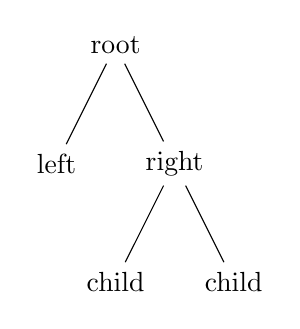
\begin{tikzpicture}
  \node {root}
    child {node {left}}
    child {node {right}
      child {node {child}}
      child {node {child}}
    };
\end{tikzpicture}

A simple image is \tikz \fill (0,0) circle(5pt);.

Furthermore, we might want to draw \tikz[baseline]\draw (0,-1) rectangle (1,1);
\end{document}
\end{codeexample}
%
\noindent where the following files are necessary to compile the document:
%
\begin{codeexample}[code only, tikz syntax=false]
tikzexternal.sty
main.tex
main-figure0.pdf
main-figure1.pdf
main-figure2.pdf
\end{codeexample}
%
\noindent If there are any `|.dpth|' files, for example |main-figure2.dpth|,
these files are also required. They contain information for the \tikzname\
|baseline| option (or |\label|s inside external graphics).

Just copy the |.sty| file into the directory of your |main.tex| file and use it
as part of your document.

Please keep in mind, that only |tikzpicture| environments and |\tikz| short
images are available within the externalization framework. Additionally, calls
to |\tikzset| and |\pgfkeys| won't lead to compilation errors because they are
simply ignored. But since |pgfkeys| is not available, any option supplied to
|\tikzexternalize| is \emph{ignored}.

\paragraph{Attention:}
Since the simple replacement |\usepackage{tikzexternal}| doesn't support the
key--value interface, you \emph{need} to use |\tikzsetexternalprefix| instead
of the |prefix| option and |\tikzsetfigurename| instead of the |figure name|
option since |\tikzset| is not available in such a context.

\paragraph{Remark:}
Some of the features of this library are mainly useful to improve the speed of
successive document compilations. In other words: you can't use all features in
this context, keep it simple.


\subsection{\texttt{eps} Graphics Export}

It is also possible to use \eps\ graphics instead of \pdf\ files. There are
different ways to produce them, for example to use |pdflatex| and call
|pdftops -eps |\marg{pdf file} \marg{eps file} afterwards. You could add this
command to the |system call| option.

Alternatively, you can use |latex| and |dvips| for image conversion as is
explained for the |system call| option, see
page~\pageref{extlib:systemcall:option}. See the documentation for the basic
level externalization in section~\ref{section-external} for restrictions of
other drivers.


\subsection{Bitmap Graphics Export}

Occasionally, you may have an extremely large graphics which takes long times
to render. It might be interesting to generate a bitmap (raster) image, which
displays much faster (for example in a presentation). I have used this feature
to speed-up the display of large shadings.

The |external| library can be customized to export bitmap images -- with the
help of external programs. Due to the dependence of external programs, you may
need to adjust these commands manually. For example, on my computer, the
ImageMagick Suite is installed which comes with the |convert| tool. Together
with |pdflatex|, I can define the following style:
%
\begin{codeexample}[code only]
\tikzset{
    % Defines a custom style which generates BOTH, .pdf and .png export
    % but prefers the .png on inclusion.
    %
    % This style is not pre-defined, you may need to copy-paste and
    % adjust it.
    png export/.style={
        external/system call/.append=
            {; convert -density 300 -transparent white "\image.pdf" "\image.png"},
        %
        /pgf/images/external info,
        /pgf/images/include external/.code={%
            \includegraphics
                [width=\pgfexternalwidth,height=\pgfexternalheight]
                {##1.png}%
        },
    }
}
\end{codeexample}
%
\noindent The example above defines a new style called `|png export|' which,
when it is set with |\tikzset{png export}| somewhere in the document, modifies
the configuration for both file generation and file input. The file generation
is modified by appending the ImageMagick command to |system call| (separated by
`|;|' as usual on Linux). This is, in principle, enough to generate a |.png|
file. The |include external| command is overwritten such that it uses the
|.png| file instead of the |.pdf| file (which exists as well in the
configuration above). But since a |.png| file can have a much higher resolution
than the desired image dimensions, we have to add |width| and |height|
explicitly. Usually, the |external| library does not provide size information
(it is unnecessary for |.pdf| or |.eps| since these formats have their bounding
box information). To enable size information, the style uses the
|external info| key, which, in turn, provides the |\pgfexternalwidth| and
|\pgfexternalheight| commands.

Now we can use |\tikzset{png export}| either document-wide or just for one
particular image. The configuration remains in effect until the end of the
current environment (or until the next closing curly brace `|}|').

\begin{key}{/pgf/images/external info=\marg{boolean} (initially false)}
    If this key is activated, the size for any externalized image will be
    stored explicitly into the associated |.dpth| file.

    When the file is included by |\pgfincludeexternalgraphics| (or
    automatically by the |external| library), the width is available as
    \declareandlabel{\pgfexternalwidth} and the height as
    \declareandlabel{\pgfexternalheight}.
\end{key}


\subsection{Compatibility Issues}

\subsubsection{References In External Pictures}

It is allowed if a picture contains references, for example
|\tikz \node {Reference to \ref{a:label}};|.

There is just one issue: if the main job is currently compiling, its |.aux|
file is not in its final state (even worse: it may not be readable at all). The
picture externalization, however, needs the main |.aux| file to query any
references.

Thus, you \emph{will} need to invoke
|pdflatex -jobname |\meta{image}| |\meta{mainfile} \emph{manually}
for any image which contains references.

This problem arises only for |mode=convert with system call|. In this case,
the |external| library creates a special |\jobname.auxlock| file to check
whether the main |.aux| file is currently usable.


\subsubsection{Compatibility With Other Libraries or Packages}

The |external| library has the following compatibility issues:
%
\begin{enumerate}
    \item The |external| library comes with special support for
        |\usetikzlibrary{fadings}|: the |fadings| library may define local
        pictures which would be externalized (although they shouldn't). There
        is special handling to suppress this bug if |\tikzexternalize| is
        called \emph{after} |\usetikzlibrary{fadings}| or if all fadings are
        defined \emph{before} |\tikzexternalize|.
    \item Problems have been reported when using |\tikzexternalize| (or the
        basic layer externalization) together with |\usepackage{glossary}|.
        This problem disappears if |\tikzexternalize| is called \emph{before}
        |\usepackage{glossary}|.
    \item Problems with |\usepackage{pdfpages}| and |\usepackage{vmargin}|: The
        |external| library replaces the current shipout routine of \TeX\ during
        its externalization. This might raise problems with other packages
        which also manipulate the shipout routine (like the mentioned ones). To
        fix those problems, use
        %
\begin{codeexample}[code only]

\usetikzlibrary{external}

\tikzifexternalizing{%
    % don't include package XYZ here
}{%
    \usepackage{pdfpages}
    \usepackage{vmargin}
    ...
}%
\end{codeexample}
        %
        This uses the requested packages for the main document, but not for the
        single, exported graphics.
\end{enumerate}

In general, the |\tikzifexternalizing| feature might be used to solve package
conflicts and the |\tikzexternaldisable| and |\tikzexternalenable| features can
be used to solve problems with single pictures.


\subsubsection{Compatibility With Bounding Box Restrictions}

Bounding box restrictions provide no problem when used with \eps\ graphics.
However, they pose problems for |pdflatex|, so you may need to use the
|latex|/|dvips| combination if you use bounding box restrictions and
externalization. Currently, the only possibility for bounding box restrictions
and |pdflatex| is to use a combination of |trim left|/|trim right|/|baseline|:
these keys do not \emph{really} truncate the bounding box, they only store
horizontal and vertical shifts (also see the |trim lowlevel| key in this
context).


\subsubsection{Interoperability With The Basic Layer Externalization}

This library is fully compatible with
|\beginpgfgraphicnamed|$\dotsc$|\endpgfgraphicnamed| environments. However, you
will need to use the |export next=false| key to avoid conflicts:
%
\begin{codeexample}[code only]
\beginpgfgraphicnamed{picture4}
\tikzset{external/export next=false}
\begin{tikzpicture}
   \draw (0,0) -- (4,4);
\end{tikzpicture}
\endpgfgraphicnamed
\end{codeexample}
%
Please keep in mind that file prefixes do not apply to the basic layer.
}
